 % For printing in a4
\documentclass[a4,10pt,twoside,openright,italian,english]{book}% twoside!

% For printing with the A5 format
%\documentclass[10pt,twoside,openright,english,italian]{book}% twoside!

% Set paper size
\usepackage[twoside=true]{geometry}

%For printing with the weird format
%\geometry{
%	paperwidth=17cm,
%	paperheight=24cm,
%	margin=2cm,
%	top=2.3cm,
%	bindingoffset=0.4cm
%}
% For printing in a4
\geometry{a4paper,
  margin=3cm,
  top=3.8cm,
  bindingoffset=0.4cm
}

%Uncomment this for final prints: this just enables printing on a4 paper
\usepackage[cam,center,a4,pdflatex,axes]{crop}

\usepackage{phdthesis}

\usepackage{fancyhdr}
\usepackage{color}
\usepackage{array}
\usepackage{mdwmath}
\usepackage{mdwtab}
\usepackage{amsmath,amssymb}
\usepackage{cite}
\usepackage{graphicx}
\usepackage{listings}
\usepackage{subfig}
\usepackage{booktabs}
\usepackage{latexsym}
\usepackage{color}
\usepackage{url}
\usepackage{bnf}
\usepackage{rotating}
\usepackage{multirow}
\usepackage{multicol}
\usepackage{phdtitle}
\usepackage{paralist}
\usepackage{bibentry}
\usepackage{xcolor}
\usepackage{pifont} 
\usepackage[algochapter]{algorithm2e}
\usepackage[bookmarks=true,
%pdftex=false,
bookmarksopen=true,hidelinks]{hyperref}
\usepackage[toc,acronym]{glossaries}
\usepackage{lscape}
\usepackage{algorithmic}
\usepackage{algorithm}
\usepackage{longtable}
\usepackage[T1]{fontenc} 
%\usepackage[latin1]{inputenc}
\usepackage[utf8]{inputenc}
%\usepackage{fontspec}
%\setmainfont{Calibri}
\usepackage{cleveref}
\usepackage{enumitem}

\usepackage{smartdiagram}
\usesmartdiagramlibrary{additions}
\usepackage{tikz}
\usetikzlibrary{shapes.geometric}
\usetikzlibrary{shapes.arrows}
\usetikzlibrary{arrows, backgrounds, calc, hobby, positioning, chains}

\newcounter{sdpic}
\hyphenation{man-u-scripts}

%% \hyphenation{} is used to force the 
\hyphenation{}

\newtheorem{Definition}{Definition}[section]

% Define custom colors if needed
\definecolor{BurntOrange}{RGB}{204,85,0}
\definecolor{MidnightBlue}{RGB}{25,25,112}
\definecolor{Maroon}{RGB}{128,0,0}
\definecolor{CustomGreen}{RGB}{143, 209, 79}
\definecolor{CustomBlue}{RGB}{45, 155, 240}
\definecolor{CustomYellow}{RGB}{250, 199, 16}

\definecolor{codegreen}{rgb}{0,0.6,0}
\definecolor{codegray}{rgb}{0.5,0.5,0.5}
\definecolor{codepurple}{rgb}{0.58,0,0.82}
\definecolor{backcolour}{rgb}{0.95,0.95,0.92}

\lstdefinestyle{mystyle}{
    backgroundcolor=\color{backcolour},   
    commentstyle=\color{codegreen},
    keywordstyle=\color{magenta},
    numberstyle=\tiny\color{codegray},
    stringstyle=\color{codepurple},
    basicstyle=\ttfamily\footnotesize,
    breakatwhitespace=false,         
    breaklines=true,                 
    captionpos=b,                    
    keepspaces=true,                 
    numbers=left,                    
    numbersep=5pt,                  
    showspaces=false,                
    showstringspaces=false,
    showtabs=false,                  
    tabsize=2
}

\lstset{style=mystyle}

% \lstset{tabsize=2,basicstyle=\footnotesize,breaklines=true}
\lstset{escapeinside={/*!}{!*/}}

\usepackage[english,italian]{babel}
\usepackage{ulem}
\normalem

\hypersetup{pdftitle={Title}, pdfauthor={Author}}

\nobibliography*

\department {Dottorato di ricerca in Ingegneria dell'Informazione}

% Please fulfil the followed fields with your data
\author{Nicolò Pratelli} 
\title{Formal Representation of Geospatial Knowledge in Narratives}
\tutor{Antonella Poggi\\ Prof. Ricardo Nuno Taborda Campos}
\supervisor{Nicola Tonellotto\\Dr. Valentina Bartalesi Lenzi}
\titleimage{img/unipi.png} %please not change
\phdyear{2025}
\phdmonth{January}
\phdcycle{XXXVII Cycle}

%%%%%%%%%%%%%%%%%%%%%%%%%%%%%%%%%%%%%%
% Let's Start The Real Document
%%%%%%%%%%%%%%%%%%%%%%%%%%%%%%%%%%%%%%
% \newglossaryentry{matrix_channel}
% {       name={$H^*$},
%         description={Conjugate operation}
% }
% \newglossaryentry{trasp_x}
% {       name={$[ x ]^{\rm T}$},
%         description={transpose operator}
% }
% \newglossaryentry{vec_x}
% {       name={\textbf{x}},
%         description={vectors are in bold}
% }
% \newglossaryentry{floor_funct}
% {       name={$\left\lfloor x \right\rfloor$},
%         description={round to the lower integer of $x$}
% }

% PREFIXES

\newglossaryentry{ogc}
{       name={ogc:},
        description={\texttt{http://www.opengis.net/}}
}

\newglossaryentry{geo}
{       name={geo:},
        description={\texttt{http://www.opengis.net/ont/geosparql#}}
}

\newglossaryentry{geof}
{       name={geof:},
        description={\texttt{http://www.opengis.net/def/function/geosparql/}}
}

\newglossaryentry{geor}
{       name={geor:},
        description={\texttt{http://www.opengis.net/def/rule/geosparql/}}
}

\newglossaryentry{rdf}
{       name={rdf:},
        description={\texttt{http://www.w3.org/1999/02/22-rdf-syntax-ns#}}
}

\newglossaryentry{rdfs}
{       name={rdfs:},
        description={\texttt{http://www.w3.org/2000/01/rdf-schema#}}
}

\newglossaryentry{xsd}
{       name={xsd:},
        description={\texttt{http://www.w3.org/2001/XMLSchema#}}
}

\newglossaryentry{owl}
{       name={owl:},
        description={\texttt{http://www.w3.org/2002/07/owl#}}
}

\newglossaryentry{schema}
{       name={schema:},
        description={\texttt{http://schema.org/}}
}

\newglossaryentry{strdf}
{       name={strdf:},
        description={\texttt{http://strdf.di.uoa.gr/ontology#}}
}

\newglossaryentry{ecrm}
{       name={ecrm:},
        description={\texttt{http://erlangen-crm.org/current/}}
}

\newglossaryentry{crmgeo}
{       name={crmgeo:},
        description={\texttt{http://www.ics.forth.gr/isl/CRMgeo/}}
}

\newglossaryentry{narra}
{       name={narra:},
        description={\texttt{https://dlnarratives.eu/ontology#}}
}

\newglossaryentry{igen}
{       name={igen:},
        description={\texttt{https://imagoarchive.it/thes/tid/}}
}

\newglossaryentry{ilrm}
{       name={ilrm:},
        description={\texttt{http://imagoarchive.it/ilrmoo/}}
}

\newglossaryentry{wdt}
{       name={wdt:},
        description={\texttt{http://www.wikidata.org/prop/direct/}}
}
\newglossaryentry{wd}
{       name={wd:},
        description={\texttt{http://www.wikidata.org/entity/}}
}

\newglossaryentry{uom}
{       name={uom:},
        description={\texttt{http://www.opengis.net/def/uom/OGC/1.0/}}
}

\newglossaryentry{osm}
{       name={osm:},
        description={\texttt{https://www.openstreetmap.org/}}
}

\newglossaryentry{osm2rdfkey}
{       name={osm2rdfkey:},
        description={\texttt{https://osm2rdf.cs.uni-freiburg.de/rdf/key#}}
}

\newglossaryentry{osmkey}
{       name={osmkey:},
        description={\texttt{https://www.openstreetmap.org/wiki/Key:}}
}

\newglossaryentry{imago}
{       name={imago:},
        description={\texttt{https://imagoarchive.it/ontology/}}
}










% ogc: http://www.opengis.net/
% geo: http://www.opengis.net/ont/geosparql#
% geof: http://www.opengis.net/def/function/geosparql/
% geor: http://www.opengis.net/def/rule/geosparql/
% sf: http://www.opengis.net/ont/sf#
% gml: http://www.opengis.net/ont/gml#
% xsd: http://www.w3.org/2001/XMLSchema#
% rdf: http://www.w3.org/1999/02/22-rdf-syntax-ns#
% rdfs: http://www.w3.org/2000/01/rdf-schema#
% owl: http://www.w3.org/2002/07/owl#
\newacronym[longplural={geographic information systems}]{GISLabel}{GIS}{geographic information systems}
\newacronym[longplural={Resource Description Framework}]{RDFLabel}{RDF}{Resource Description Framework}
\newacronym[longplural={Resource Description Framework Schema}]{RDFSLabel}{RDFS}{Resource Description Framework Schema}
\newacronym[longplural={Web Ontology Language}]{OWLLabel}{OWL}{Web Ontology Language}
\newacronym[longplural={SPARQL Protocol and RDF Query Language }]{SPARQLLabel}{SPARQL}{SPARQL Protocol and RDF Query Language }
\newacronym[longplural={Uniform Resource Identifiers}]{URILabel}{URI}{Uniform Resource Identifier}
\newacronym[longplural={Internationalized Resource Identifiers}]{IRILabel}{IRI}{Internationalized Resource Identifier}
\newacronym[longplural={Linked Open Data}]{LODLabel}{LOD}{Linked Open Data}
\newacronym[longplural={Terse RDF Triple Language}]{TurtleLabel}{Turtle}{Terse RDF Triple Language}
\newacronym[longplural={Coordinate Reference Systems}]{CRSLabel}{CRS}{Coordinate Reference System}
\newacronym[longplural={Region Connection Calculus}]{RCCLabel}{RCC}{Region Connection Calculus}
\newacronym[longplural={jointly exhaustive and pairwise disjoint}]{JEPDLabel}{JEPD}{jointly exhaustive and pairwise disjoint}
\newacronym[longplural={9-intersection model}]{9IMLabel}{9IM}{9-intersection model}
\newacronym[longplural={dimensionally extended 9-intersection model}]{DE9IMLabel}{DE9IM}{dimensionally extended 9-intersection model}
\newacronym[longplural={4-intersection model}]{4IMLabel}{4IM}{4-intersection model}
\newacronym[longplural={Open Geospatial Consortium}]{OGCLabel}{OGC}{Open Geospatial Consortium}
\newacronym[longplural={Event Calculus}]{ECLabel}{EC}{Event Calculus}
\newacronym[longplural={Descriptive Ontology for Linguistic and Cognitive Engineering}]{DOLCELabel}{DOLCE}{Descriptive Ontology for Linguistic and Cognitive Engineering}
\newacronym[longplural={Well-Known Text}]{WKTLabel}{WKT}{Well-Known Text}
\newacronym[longplural={Geography Markup Language}]{GMLLabel}{GML}{Geography Markup Language}
\newacronym[longplural={International Committee for Documentation}]{CIDOCLabel}{CIDOC}{International Committee for Documentation}
\newacronym[longplural={Conceptual Reference Model}]{CRMLabel}{CRM}{Conceptual Reference Model}
\newacronym[longplural={CIDOC Conceptual Reference Model}]{CIDOCCRMLabel}{CIDOC CRM}{CIDOC Conceptual Reference Model}
\newacronym[longplural={Narrative Ontology}]{NOntLabel}{NOnt}{Narrative Ontology}
\newacronym[longplural={Geospatial Narrative Ontology}]{NOnt+SLabel}{NOnt+S}{Geospatial Narrative Ontology}
\newacronym[longplural={Semantic Web Rule Language}]{SWRLLabel}{SWRL}{Semantic Web Rule Language}
\newacronym[longplural={Value Chains}]{VCLabel}{VC}{Value Chain}
\newacronym[longplural={Local Administrative Units}]{LAULabel}{LAU}{Local Administrative Unit}
\newacronym[longplural={Nomenclature of Territorial Units for Statistics}]{NUTSLabel}{NUTS}{Nomenclature of Territorial Units for Statistics}
\newacronym[longplural={Findable, Accessible, Interoperable, and Reusable}]{FAIRLabel}{FAIR}{Findable, Accessible, Interoperable, and Reusable}
\newacronym[longplural={Story Map Building And Visualising Tool}]{SMBVTLabel}{SMBVT}{Story Map Building And Visualising Tool}
\newacronym[longplural={LinkedGeoData}]{LGDLabel}{LGD}{LinkedGeoData}
\newacronym[longplural={OpenStreetMap}]{OSMLabel}{OSM}{OpenStreetMap}
\newacronym[longplural={Greek Administrative Geography}]{GAGLabel}{GAG}{Greek Administrative Geography}
\newacronym[longplural={CORINE Land Cover}]{CLCLabel}{CLC}{CORINE Land Cover}
\newacronym[longplural={Earth Observation}]{EOLabel}{EO}{Earth Observation}
\newacronym[longplural={Non-Topological Construct Functions}]{NTCFLabel}{NTCF}{Non-Topological Construct Functions}
\newacronym[longplural={Spatial Selections}]{SSLabel}{SS}{Spatial Selections}
\newacronym[longplural={Spatial Joins}]{SJLabel}{SJ}{Spatial Joins}
\newacronym[longplural={Geographic Information System of the Commission}]{GISCOLabel}{GISCO}{Geographic Information System of the Commission}
\newacronym[longplural={MOuntain Valorisation through INterconnectedness and Green growth}]{MOVINGLabel}{MOVING}{MOuntain Valorisation through INterconnectedness and Green growth}
\newacronym[longplural={Index Medii Aevi Geographiae Operum}]{IMAGOLabel}{IMAGO}{Index Medii Aevi Geographiae Operum}


\makeglossaries

\begin{document}
\selectlanguage{english}

\maketitle

\pagestyle{empty}

\cleardoublepage
\newpage

%%%%%%%%%%%%%%%%%%%%%%%%%%%%%%%%%%%%%%
% Dedication - For removing dedication, please comment or delete the code inside \thispagestyle{empty}
%%%%%%%%%%%%%%%%%%%%%%%%%%%%%%%%%%%%%%
\thispagestyle{empty}
    \null\vspace{\stretch {1}}
        \begin{flushright}
                This thesis is dedicated to....
        \end{flushright}
\vspace{\stretch{2}}\null

\cleardoublepage
\newpage

\pagestyle{empty}
%% change numbering into Roman numbers for the introductory part
%\setcounter{page}{1}
%\pagenumbering{Roman}

%%%%%%%%%%%%%%%%%%%%%%%%%%%%%%%%%%%%%%
% Quotes - For removing quotes, please comment or delete the code inside \thispagestyle{empty}
%%%%%%%%%%%%%%%%%%%%%%%%%%%%%%%%%%%%%%
\thispagestyle{empty}
    \null\vspace{\stretch {1}}
        \begin{flushright}
                "Home is behind, the world ahead, \\
                and there are many paths to tread \\
                through shadows to the edge of night,\\
                until the stars are all alight"\\
                J.R.R. Tolkien, The Lord of the Rings
                % "A few first rate research papers are preferable to a large number \\
                % that are poorly conceived or half-finished.\\
                % The latter are no credit to their writers and \\
                % a waste of time to their readers"\\
                % Claude Shannon
                %IRE Transactions on Information Theory (1956), volume 2, issue 1, page 3. Shannon, Claude E. (March 1956), The Bandwagon, 2, doi:10.1109/TIT.1956.1056774.
        \end{flushright}
\vspace{\stretch{2}}\null

\cleardoublepage
\newpage

\pagestyle{empty}
%% change numbering into Roman numbers for the introductory part
\setcounter{page}{1}
\pagenumbering{Roman}

%%%%%%%%%%%%%%%%%%%%%%%%%%%%%%%%%%%%%%
% Acknowledgement
%%%%%%%%%%%%%%%%%%%%%%%%%%%%%%%%%%%%%%
\chapter*{Acknowledgements}
\lettrine{A}{cknowledgements} goes here.

\selectlanguage{italian}
\chapter*{Ringraziamenti}
\lettrine{R}{ingraziamenti} 
\selectlanguage{english}

\cleardoublepage
\newpage

\pagestyle{fancy}
% change numbering into Roman numbers for the introductory part

%%%%%%%%%%%%%%%%%%%%%%%%%%%%%%%%%%%%%%
% Summary
%%%%%%%%%%%%%%%%%%%%%%%%%%%%%%%%%%%%%%
\selectlanguage{english}
\chapter*{Summary}

\lettrine{G}{eospatial} knowledge plays a fundamental role in shaping the understanding and communication of narratives. Whether historical, literary, or journalistic, narratives often incorporate spatial elements that provide essential context, enriching the reader’s engagement with the story. This thesis addresses a fundamental challenge in the fields of knowledge representation and the Semantic Web: the effective semantic modeling of geospatial narratives. Geospatial narratives are conceived as networks of events interconnected through semantic links, capturing the complex relationships between spatial occurrences. Current models lack sufficient expressiveness and interoperability, which limits their capacity for data integration, querying, and analysis. To overcome these limitations, this research develops the Geospatial Narrative Ontology (NOnt+S), an extension of the existing Narrative Ontology (NOnt) that is based on the ISO standard CIDOC Conceptual Reference Model (CIDOC CRM). By formally modeling geospatial information using a formal language like OWL 2 DL, the ontology ensures decidability and enhances interoperability across diverse knowledge bases. Furthermore, implementing this ontology within a Semantic Web framework and employing semantic reasoners enable the inference of new geospatial knowledge, thereby enriching data analysis and facilitating more sophisticated queries. Finally, the thesis addresses the challenges of visualization by proposing Story Maps as a solution to visualize geospatial narratives. Story Maps are interactive digital maps that tell stories by integrating geospatial data with narrative elements. Story mapping, in this context, is a method for arranging narrative events to create a more holistic view of how they fit into the overall geospatial narrative, thereby enhancing user engagement and understanding.

\section*{Research Objectives}

The thesis aims to advance geospatial knowledge representation in narratives by:
\begin{enumerate}
    \item Developing an ontology, NOnt+S, wich representan geospatial and temporal aspects of narratives ensuring interoperability with existing Semantic Web frameworks.
    \item Enhancing data integration and enabling advanced geospatial querying mechanisms to achieve consistent and comprehensive representations of geospatial information in narratives.
    \item Evaluating the ontology's practical implications and applicability, including its ability to infer new knowledge, through empirical validation in real-world case studies from the MOVING (Horizon 2020-2024) and IMAGO (PRIN 2020-2024) projects.
    \item Developing effective visualization methods for geospatial narratives by employing Story Maps, integrating geospatial data with narrative elements to enhance user understanding and engagement.
\end{enumerate}

\section*{Methodology}

The research employs a rigorous, structured methodology based on the METHONTOLOGY framework, which includes:
\begin{itemize}
    \item \textbf{Requirements Specification}: Identifying the requirements for geospatial narrative representation through comprehensive analysis.
    \item \textbf{Conceptualization and Logical Formalization}: Extending the NOnt ontology to incorporate geospatial and temporal constructs, providing formal mathematical specifications.
    \item \textbf{Implementation}: Developing NOnt+S in OWL 2 DL, ensuring decidability and interoperability to achieve syntactic precision and compatibility within the Semantic Web environment.
    \item \textbf{Evaluation}: Validating the ontology through case studies, assessing its performance in terms of semantic enrichment, reasoning capabilities, and querying effectiveness.
\end{itemize}

\section*{Significance of Findings}
This thesis advances Knowledge Representation by introducing the NOnt+S ontology, a robust framework for modeling complex geospatial narrative structures. NOnt+S integrates narrative elements like fabula (chronological sequence) and plot (narrative presentation) with spatial constructs such as qualitative and quantitavce place. By bridging narrative and spatial dimensions, it addresses limitations in existing ontologies and sets a new standard for flexible modeling applicable in digital humanities, GIS, and smart city applications.

Adopting established standards like the CIDOC CRM and GeoSPARQL ensures interoperability with existing data systems and semantic web technologies. An embedded semantic reasoner allows NOnt+S to infer new knowledge from existing data, uncovering hidden patterns within narrative and spatial information.

The study also developed a software architecture utilizing Story Maps, providing an intuitive interface for visualizing geospatial narratives by integrating text, images, and maps. By supporting the construction of structured geospatial knowledge graphs and aligning with Linked Open Data principles, NOnt+S promotes data reusability and interdisciplinary collaboration. Validated across diverse domains, it demonstrates effectiveness in managing intricate geospatial queries and serves as a significant asset for advanced geospatial narrative modeling, laying the groundwork for future advancements.


\selectlanguage{english}

%%%%%%%%%%%%%%%%%%%%%%%%%%%%%%%%%%%%%%
% Italian Summary
%%%%%%%%%%%%%%%%%%%%%%%%%%%%%%%%%%%%%%

%There must be an Italian version of the summary
\selectlanguage{italian}
\chapter*{Sommario}
\lettrine{L}{a} conoscenza geospaziale ha un impatto significativo sulla comprensione e sulla comunicazione delle storie. Le narrazioni — che siano di natura storica, letteraria o giornalistica — spesso includono elementi spaziali che offrono un contesto fondamentale per la comprensione del racconto. Questa tesi affronta una sfida fondamentale nei campi della rappresentazione della conoscenza e del Web Semantico: la modellazione semantica delle narrazioni geospaziali. Le narrazioni geospaziali sono concepite come reti di eventi interconnessi attraverso legami semantici, catturando le complesse relazioni tra le occorrenze spaziali. I modelli attuali mancano di sufficiente espressività e interoperabilità, il che limita la loro capacità di integrazione dei dati, interrogazione e analisi. Per superare queste limitazioni, questa ricerca sviluppa l'Ontologia delle Narrazioni Geospaziali (NOnt+S), un'estensione dell'esistente Ontologia delle Narrazioni (NOnt) che si basa sullo standard ISO CIDOC Conceptual Reference Model (CIDOC CRM). La modellazione formale delle informazioni geospaziali tramite un linguaggio formale come OWL 2 DL garantisce la decidibilità e migliora l'interoperabilità tra diverse basi di conoscenza. Inoltre, implementando questa ontologia all'interno di un framework del Web Semantico e impiegando ragionatori semantici, si rende possibile l'inferenza di nuova conoscenza geospaziale, arricchendo così l'analisi dei dati e facilitando interrogazioni più sofisticate. Infine, la tesi affronta le sfida di una visualizzazione efficace proponendo le \textit{Story Maps} come soluzione per visualizzare le narrazioni geospaziali. Le \textit{Story Maps} sono mappe digitali interattive che raccontano storie integrando dati geospaziali con elementi narrativi. Lo \textit{story mapping}, in questo contesto, è un metodo per organizzare gli eventi narrativi al fine di creare una visione più olistica di come essi si inseriscono nella narrazione geospaziale complessiva, migliorando così il coinvolgimento e la comprensione dell'utente.

\section*{Obiettivi della ricerca}

La tesi mira ad avanzare la rappresentazione della conoscenza geospaziale nelle narrazioni proponendosi di:

\begin{enumerate}
    \item Sviluppare un'ontologia, NOnt+S, che rappresenta gli aspetti geospaziali e temporali delle narrazioni, garantendo l'interoperabilità con i framework esistenti del Web Semantico.
    \item Migliorare l'integrazione dei dati e abilitare sitemi di interrogazione geospaziale per ottenere rappresentazioni coerenti e complete delle informazioni geospaziali nelle narrazioni
    \item Valutare le implicazioni pratiche e l'applicabilità dell'ontologia, inclusa la sua capacità di inferire nuova conoscenza, attraverso la validazione empirica in casi di studio reali dai progetti MOVING (Horizon 2020-2024) e IMAGO (PRIN 2020-2024).
    \item Sviluppare metodi efficaci di visualizzazione per le narrazioni geospaziali utilizzando Story Maps, integrando dati geospaziali con elementi narrativi per migliorare la comprensione e il coinvolgimento dell'utente.
\end{enumerate}

\section*{Metodologia}

La ricerca impiega una metodologia rigorosa e strutturata basata sul framework METHONTOLOGY, che include:

\begin{itemize}
    \item \textbf{Specifica dei requisiti}: identificazione dei requisiti per la rappresentazione delle narrazioni geospaziali attraverso un'analisi esaustiva.
    \item \textbf{Concettualizzazione e formalizzazione logica}: estendere l'ontologia NOnt per incorporare costrutti geospaziali e temporali, fornendo una formalizzazione matematica.
    \item \textbf{Implementazione}: sviluppare NOnt+S in OWL 2 DL, garantendo decidibilità e interoperabilità per ottenere precisione sintattica e interoperabilità all'interno del Web Semantico.
    \item \textbf{Valutazione}: validare l'ontologia attraverso casi di studio, valutando le sue prestazioni in termini di arricchimento semantico, capacità di ragionamento ed efficacia nelle interrogazioni.
\end{itemize}

\section*{Importanza dei risultati}

Questa tesi avanza la rappresentazione della conoscenza introducendo l'ontologia NOnt+S, un framework robusto per modellare narrazioni geospaziali complesse. NOnt+S integra elementi narrativi come la fabula (sequenza cronologica) e l'intreccio (presentazione narrativa) con costrutti spaziali quali i luoghi qualitativi e quantitativi. Collegando le dimensioni narrative e spaziali, affronta le limitazioni delle ontologie esistenti e stabilisce un nuovo standard per la modellazione flessibile applicabile nelle \textit{digital humanities}, nei GIS e nelle applicazioni per le smart city.

Adottando standard consolidati come il CIDOC CCnceptual Reference Model (CIDOC CRM) e GeoSPARQL, si garantisce l'interoperabilità con i dati esistenti e le tecnologie del Web Semantico. Tramite un ragionatore semantico integrato, NOnt+S è in grado di inferire nuova conoscenza dai dati esistenti, rivelando pattern nascosti all'interno delle informazioni narrative e geospaziali.

Lo studio ha inoltre sviluppato un \textit{framework} software che utilizza Story Maps, fornendo un'interfaccia intuitiva per visualizzare narrazioni geospaziali attraverso l'integrazione di testo, immagini e mappe. Supportando la costruzione di grafi di conoscenza geospaziale strutturati e allineandosi ai principi dei Linked Open Data (LOD), NOnt+S promuove la riutilizzabilità dei dati e la collaborazione interdisciplinare. Validata in domini diversi, dimostra efficacia nella gestione di interrogazioni geospaziali complesse e rappresenta una risorsa significativa per la modellazione avanzata di narrazioni geospaziali, gettando le basi per futuri progressi.
\selectlanguage{english}

%%%%%%%%%%%%%%%%%%%%%%%%%%%%%%%%%%%%%%
% Publications
%%%%%%%%%%%%%%%%%%%%%%%%%%%%%%%%%%%%%%

%List of publications of the PhD candidate
\selectlanguage{english}
\chapter*{List of publications}

\section*{International Journals}
\begin{enumerate}
    % for citing your paper, take directly APA format from Google scholar
    % \item Surname, N., Surname, N. and Surname, N. (Year,Month). Title of the paper or journal. \emph{Place of publication}. (Vol. 123, pp. 456). EditorName.
    \item Bartalesi, V., Pratelli, N. (2024) Representing Geospatial Knowledge in Narratives.  \emph{ACM Journal on Computing and Cultural Heritage}, Just Accepted (November 2024).
    \item Bartalesi, V., Coro, G., Lenzi, E., Pratelli, N., Pagano, P., Moretti, M., Brunori, G. (2024). A Semantic Knowledge Graph of European Mountain Value Chains. \emph{Scientific Data}, 11(1), 978.
    \item Zabulis, X., Partarakis, N., Bartalesi, V., Pratelli, N., Meghini, C., Dubois, A., Moreno, I., Manitsaris, S. (2024). Multimodal Dictionaries for Traditional Craft Education. \emph{Multimodal Technologies and Interaction}, 8(7), 63.
    \item Zabulis, X., Partarakis, N., Demeridou, I., Bartalesi, V., Pratelli, N., Meghini, C., Nikolaou, N.,  Fallahian, P. (2024). Modelling and Simulation of Traditional Craft Actions. \emph{Applied Sciences}, 14(17), 7750.
    \item Bartalesi, V., Coro, G., Lenzi, E., Pagano, P., Pratelli, N. (2023). From unstructured texts to semantic story maps. \emph{International Journal of Digital Earth}, 16(1), 234–250.
    \item Bartalesi, V., Coro, G., Lenzi, E., Pratelli, N., Pagano, P., Felici, F., Moretti, M., Brunori, G. (2023). Using semantic story maps to describe a territory beyond its map. \emph{Semantic Web}, 14(6), 1255–1272.
    \item Bartalesi, V., Pratelli, N., Lenzi, E., Pontari, P. (2023). Using Semantic Web to Create and Explore an Index of Toponyms Cited in Medieval Geographical Works. \emph{ACM Journal on Computing and Cultural Heritage}, 16(2), 1–18.
    \item Zabulis, X., Partarakis, N., Demeridou, I., Doulgeraki, P., Zidianakis, E., Argyros, A., Theodoridou, M., Marketakis, Y., Meghini, C., Bartalesi, V. (2023). A roadmap for craft understanding, education, training, and preservation. \emph{Heritage}, 6(7), 5305–5328.
    \item Bartalesi, V., Metilli, D., Pratelli, N.,  Pontari, P. (2022). Towards a knowledge base of medieval and renaissance geographical Latin works: The IMAGO ontology. \emph{Digital Scholarship in the Humanities}, 37(1), 34–50.
    \item Bartalesi, V., Pratelli, N., Lenzi, E. (2022). Linking different scientific digital libraries in Digital Humanities: The IMAGO case study. \emph{International Journal on Digital Libraries}, 23(4), 303–317.
    \item Bartalesi, V., Pratelli, N., Meghini, C., Metilli, D., Tomazzoli, G., Livraghi, L. M., Zaccarello, M. (2022). A formal representation of the divine comedy’s primary sources: The Hypermedia Dante Network ontology. \emph{Digital Scholarship in the Humanities}, 37(3), 630–643.
\end{enumerate}

\section*{International Conferences/Workshops with Peer Review}
\begin{enumerate}
    % for citing your paper, take directly APA format from Google scholar
    % \item Surname, N., Surname, N. and Surname, N. (Year,Month). Title of the paper or journal. \emph{Place of publication}. (Vol. 123, pp. 456). EditorName.
    
    \item Bartalesi, V., Lenzi, E., Pratelli, N. (2023). A Web Tool to Create and Visualise Semantic Story Maps. 163–169.
    \item Bartalesi, V., Pratelli, N. (2021). The imago project: Towards a knowledge base of medieval and renaissance geographical works. SWODCH.
    \item Bartalesi, V., Pratelli, N., Lenzi, E. (2022). A Knowledge Base of Medieval and Renaissance Geographic Latin Works. IRCDL.
    \item Pratelli, N. (2022). A Geographical Extension for NOnt Ontology. 3246, 126–133.
\end{enumerate}

\section*{Others}
\begin{enumerate}
    % for citing your paper, take directly APA format from Google scholar
    % \item Surname, N., Surname, N. and Surname, N. (Year,Month). Title of the paper or journal. \emph{Place of publication}. (Vol. 123, pp. 456). EditorName.
    \item Bartalesi, V., Coro, G., Lenzi, E., Pratelli, N., Pagano, P. (2023). Towards Digital Twins of Territories Through Semantic Story Maps. \emph{BUILding a DIgital Twin: requirements, methods, and applications}.
    \item Bartalesi, V., Lenzi, E., Pratelli, N. (2023). Enhancing Narratives in Digital Humanities: Harnessing the Capabilities of Semantic Story Maps. Life Narrative and the Digital 2023.
\end{enumerate}















\selectlanguage{english}

%%%%%%%%%%%%%%%%%%%%%%%%%%%%%%%%%%%%%%
% List of Abbreviation and Symbols
%%%%%%%%%%%%%%%%%%%%%%%%%%%%%%%%%%%%%%
%Have a look at \gls command... you can refer a term in multiple ways
\printglossary[type=\acronymtype,title=List of Abbreviations]
\let\cleardoublepage\clearpage
\printglossary[title=Prefixes]
\cleardoublepage
\newpage
%%%%%%%%%%%%%%%%%%%%%%%%%%%%%%%%%%%%%%
% TOC
%%%%%%%%%%%%%%%%%%%%%%%%%%%%%%%%%%%%%%
\tableofcontents
\cleardoublepage
\newpage

% Now lets go back to normal numbering
\setcounter{page}{1}
\pagenumbering{arabic}

\cleardoublepage
\chapter{Title chapter 1}

%============================= INTRODUCTION =================================
\section{Introduction}\label{sec:i}
Remember that wherever you want you can cite with \verb.\cite{a1}. \cite{a1}, \cite{b1} and/or \cite{m1} someone.
Or use \verb.\footnote{That's a footnote}. like this\footnote{That's a footnote} 
% this is used to include other .tex files in order to split a long document 

%============================= SECTIONS =================================

\section{New section}
You can insert a definition
	\begin{Definition}
		Unipi: Universit\'a di Pisa
	\end{Definition}
	
\section{Another section}
	\subsection{And a subsection}
		In this sub section I will include many images just to make the list of figures meaningful.

			\begin{figure}[h!tb]
				\centerline {
\includegraphics[scale=0.6]{img/unipi.png}}
				\caption{Caption of this Unipi image.}
				\label{fig:leet}
			\end{figure}

\section{New section}
	\subsection{And also many sub}
		\subsubsection{Or again more nested}
			\begin{itemize}
				\item item 1
				\item item 2
				\item item 3
			\end{itemize}			
			
\section{New section}
This is an example of table. You can see it in Table~\ref{tab:TableName}. 

 \begin{table}[h!tb]
   \centering \caption{Table caption}
   \label{tab:TableName}
   \vskip 0.2cm
   %%
   \scalebox{0.90}{
	    %% The {|c|c|c|c|c|} define the number of columns.
	    %% c means centered
	    %% | defines a vertical line between two columns 
	    \begin{tabular}{|c|c|c|}
	      \hline
	      Col 1 & Col 2 & Col2  \\
	      %% \\ force a newline without creating an horizontal line
	      Dim C.1 & Dim C.3 & Dim C.3 \\
	      %% \hline create an horizontal line between two rows
	      \hline
	      Data 1.1 & Data 1.2 & Data 1.3 \\
	      \hline
	      Data 2.1 & Data 2.2 & Data 2.3 \\
	      \hline
	      Data 3.1 & Data 3.2 & Data 3.3 \\  
	      \hline
	    \end{tabular}
	 }
 \end{table}

\section{You can do as many section as you want}
The following equation has been created using \verb.$$.: $ y_1 = a*x + b$.

%% \smallskip introduces a small vertical skip
\smallskip

%% \noindent is used to eliminate the blankline and the paragraph settings 
\noindent
This is a more complex equation: \[ y_2 = a*x + b \], created using \verb.\[ \].

%% \bigskip introduces a big vertical skip
\bigskip

\noindent
This is, (\ref{eq:eeq1}), an enumerated equation: 

	\begin{equation}\label{eq:eeq1}
		y_3 = a*x + b
	\end{equation}

, created using:

	\begin{verbatim}
		\begin{equation}\label{eq:eeq1}
		    y_3 = a*x + b
		\end{equation}
	\end{verbatim}

It is also possible to insert acronyms, after definition in \textit{Acronyms} file, like \acrshort{fpsLabel} which stands for \acrlong{fpsLabel} or \acrshort{SNRLabel} which stands for \acrlong{SNRLabel}.
Please define the notation at the beginning, defining operators and symbols in \textit{Notation} file, such as \gls{matrix_channel}, \gls{trasp_x}, \gls{vec_x}, \gls{floor_funct}. % uncomment if you want part I
% Insert further chapters using the following syntax
% \input{Source_Folder_Name/FileName}
\chapter{Theoretical Framework}\label{chap:theoretical_framework}

\section{Introduction}\label{II-sec:introduction}

To formally represent geospatial knowledge in narratives, a comprehensive theoretical foundation is required, drawing on principles from narratology, geospatial data modeling, Semantic Web technologies, and ontology engineering. This chapter offers a detailed exploration of these foundational components, highlighting their significance in the context of geospatial narrative representation.

We begin with narratology, the study of how narratives are structured and conveyed. Tracing its roots to Aristotle’s Poetics and advancing through Russian Formalism, structuralism, and cognitive theories, narratology provides essential frameworks for understanding narrative structure. Key concepts include the distinction between \textit{fabula} (the chronological sequence of events) and \textit{syuzhet} (the narrative's presentation of those events). These concepts, along with the roles of characters and plots, are crucial for analyzing the dynamics of a narrative. Additionally, narratology offers insights into the differences between fictional narratives, which construct imagined worlds, and non-fictional narratives, grounded in real events.

Following this, we examine geospatial data modeling, beginning with the Feature-Based Approach and progressing through the Algebra and Calculi of Qualitative Spatial Relations, Topological Relations, Reasoning with Topological Relations, and Cardinal Directions. We also explore various representation techniques, such as Raster and Vector Representations, and Representation by Constraints, which are pivotal for accurately capturing spatial relationships in geospatial narratives.

Next, we introduce Semantic Web technologies, focusing on \acrshort{RDFLabel}, \acrshort{RDFSLabel}, \acrshort{OWLLabel}, and \acrshort{SPARQLLabel}. These technologies form the backbone for representing data, developing ontologies, and enabling sophisticated querying. They are integral to our research, providing the necessary infrastructure for semantic interoperability and data integration.

Finally, we turn to ontology engineering, outlining the methodologies and best practices for developing robust and interoperable ontologies. Emphasis is placed on methodological rigor, as well as the reuse of existing ontologies, to ensure efficiency and facilitate the seamless integration of diverse data sources. Through this approach, we ensure the creation of high-quality ontologies that support the formal representation of spatiotemporal narratives. 

\section{Introduction to Narratology}\label{II-sec:narratology}

Narratology is the study of narrative structures and the underlying logic, principles, and practices of their representation \cite{hermanBasicElementsNarrative2009}. Its origins trace back to Aristotle's Poetics, where narrative is described as the imitation of actions (\emph{praxis}) forming an argument (\emph{logos}), with events organized into a plot (\emph{mythos}) \cite{aristotelesPoetica2010}.

Later, Russian Formalism introduced the idea of a universal literary language or pattern of codes within a work's content, enabling narratives to be conveyed through various media like speech, writing, gestures, and music. Vladimir Propp's "Morphology of the Folktale" \cite{proppMorphologyFolktale1968} models folktales using 31 narrative functions and seven character roles or spheres of action.

Mid-20th-century structuralism further developed narratology. Claude Lévi-Strauss outlined a grammar of mythology, while A.~J.~Greimas proposed six fundamental narrative elements called \emph{actants} \cite{greimasStructuralSemanticsAttempt1983}. Tzvetan Todorov coins the term \emph{narratologie} \cite{todorovGrammaireDecameron1969}, and Gérard Genette analyzes narration separately from story content \cite{genetteNarrativeDiscourseEssay1990}.

Post-structuralist perspectives emerge in the 1980s \cite{fludernikHistoriesNarrativeTheory2005}, with Cognitive Narratology viewing narratology as a psychological phenomenon studied from a cognitive perspective \cite{davidhermanNarratologyCognitiveScience2000}. Cognitive psychology suggests that common-sense concepts often resist definition by necessary and sufficient conditions. While monotonic description logic captures aspects of conceptual knowledge, it falls short in representing prototypical knowledge; a general description logic for prototypical concepts remains undeveloped \cite{frixioneRepresentingConceptsFormal2012, lietoHybridRepresentationalProposal2014}.

\subsection{Fabula and Syuzhet}\label{II-subsec:fabulaAndSyzhet}

Russian Formalism distinguishes between \emph{fabula}, the chronological series of events at specific times and places, and \emph{syuzhet}, the author's presentation of these events \cite{proppMorphologyFolktale1968,lemonRussianFormalistCriticism1965}. Similarly, Chatman differentiates between \emph{story}, the content transmitted, and discourse, its particular organization \cite{chatmanCharactersNarratorsFilter1986}. Without a universal definition of narrative structure, some, like Crawford \cite{crawfordChrisCrawfordInteractive2012}, view narrative as a causality-based high-level structure independent of temporal or spatial relations. Genette identifies five key narrative concepts: order, frequency, duration, voice, and mood \cite{genetteNarrativeDiscourseEssay1990}. Bal adds a third level, presentation, the concrete representation of content delivered to the audience \cite{balNarratologyIntroductionTheory1997}.

\subsection{Characters and Plots}\label{II-subsec:charactersAndPlots}

Characters and plots are central to narratology. Characters, typically humans or humanoid beings, are fundamental to stories. While Aristotle emphasizes action \cite{aristotelesPoetica2010}, characters are indispensable in all tales. McKee argues that discussing plot without characters is impossible \cite{mckeeStorySubstanceStructure1997}. Chatman categorizes story elements into characters and setting elements like places and objects \cite{chatmanStoryDiscourseNarrative1978}. The plot consists of interconnected events forming a pattern within the story.

\subsection{Fictional vs. Non-fictional Narratives}\label{II-subsec:fictionalNonFictional}

A fundamental dichotomy in narratology is between fictional and non-fictional narratives \cite{jahnNarratology23Guide2021}. Fictional narratives aim to entertain and feature imaginary narrators and worlds, while Non-fictional narratives involve real-life narrators recounting actual events, such as news stories providing evidence of real occurrences.

\section{Geospatial Data Modeling}\label{II-sec:geospatialDataModeling}

This section discusses how to use mathematical abstractions to model the kinds of geospatial
information that we find in today’s applications. We consider only one way to modeling geospatial information, the feature based approach, because the field based approach is not usefult to the aim of this thesis. Then, we present three techniques for representing these abstract models in a computer: raster data, vector data, and constraints. The concept presented can also be explored in dept in Geospatial data science books, \cite{koubarakisGeospatialDataScience2023}, in \acrfull{GISLabel} books \cite{longleyGeographicInformationScience2015}, or books on geospatial DBMS \cite{rigauxSpatialDatabasesApplication2001, reveszIntroductionDatabasesBiological2010}.

\subsection{The Feature-Based Approach}\label{II-subsec:featureBased}


In \acrshort{GISLabel} terminology a geographic feature (or simply feature) is an abstraction of a real-world phenomenon and can have various attributes that describe its thematic and spatial characteristics \cite{longleyGeographicInformationScience2015}. For instance, features can represent the administrative divisions of a country, such as Italy. Thematic information about a specific administrative area, such as the municipality of Pisa, could include attributes like its name, population, and other socio-economic data. In contrast, spatial characteristics describe its geographical location and shape on Earth's surface.

Spatial attributes of a feature can be classified as either quantitative or qualitative. Quantitative spatial knowledge provides measurable data, such as distances. For example, the distance between Pisa and Florence is 90 kilometres. On the other hand, qualitative spatial knowledge refers to relational or descriptive information that cannot be easily quantified. For instance, the statement that the river Arno crosses Florence and Pisa and forms part of the border between Greece and Turkey is qualitative knowledge.

Quantitative geographic knowledge is generally represented using geometries, such as points, lines, and polygons \cite{rigauxSpatialDatabasesApplication2001, reveszIntroductionDatabasesBiological2010}. These geometries serve as abstractions of spatial features in the real world. Points can represent individual locations like cities, lines can depict rivers or roads, and polygons are used for larger areas such as administrative boundaries .

Qualitative geographic knowledge, however, is captured through qualitative binary relations between the geometries of features \cite{renzQualitativeSpatialReasoning2007}. These relations describe spatial interactions, such as adjacency or containment. For example, two polygons representing regions might share a common boundary (adjacency) or one region might be entirely contained within another .

Each geometry is associated with a \acrfull{CRSLabel}, which defines the coordinate space in which the geometry is embedded. A \acrshort{CRSLabel} uses one or more numbers, called coordinates, to uniquely specify the position of geometries within a particular space \cite{malingCoordinateSystemsMap1992}. In this thesis, we will consider Euclidean space as the coordinate system, where geometries are described and analyzed using familiar concepts from geometry and spatial mathematics.

The feature-based approach employs several classes of geometries, each suited to different types of spatial data. The geometries are displayed in figure \ref{fig:example_geometries} and can be categorized as follows::
\begin{enumerate}
    \item Point \\
    A point represents features whose shape is not of interest or that occupy an area much smaller than the space they are embedded in. Depending on the application, features like buildings, monuments, villages, or even cities can be modeled as points.

    \item Curve \\
    A curve is a one-dimensional geometry that connects points using different interpolation methods:

    \begin{itemize}
        \item Line String: A curve that uses linear interpolation between points. A line string is closed if its start and end points coincide, and simple if it has no self-intersections.
        \item Line: A line is a line string with exactly two points.
        \item Linear Ring: A line string that is both closed and simple.
    \end{itemize}

    \item Surface \\
    A surface is a two-dimensional geometry, typically represented by a single ``patch'' with one exterior boundary and zero or more interior boundaries (such as a polygon with holes). Types of surfaces include:
    
    \begin{itemize}
        \item Polygon: A simple planar surface with one exterior boundary and possibly several non-intersecting interior boundaries. It is topologically closed, and while boundaries may touch at a single point, they cannot intersect.
        \item Triangle: A specific type of polygon with three distinct, non-collinear vertices and no interior boundaries.
        \item Polyhedral Surface: A collection of polygons that share common boundary segments. Adjacent polygons share line segments, which are part of the boundary of at most two polygon patches.
        \item Triangulated Irregular Network (TIN): A polyhedral surface comprised exclusively of triangular patches.
    \end{itemize}
    
    \item Geometry Collection \\
    This is a set of distinct geometries, which can be further classified as follows:
    
    \begin{itemize}
        \item Multi-Point: A collection of points that are not connected.
        \item Multi-Curve: A collection of curves.
        \item Multi-Line String: A collection of line strings.
        \item Multi-Surface: A two-dimensional geometry collection consisting of surfaces. The geometric interiors of two surfaces may not overlap, and their boundaries may touch only at finite points.
        \item Multi-Polygon: A collection of polygons, where the boundaries of each polygon do not intersect.
    \end{itemize}

\end{enumerate}

\begin{figure}[h!tb]
    \centerline {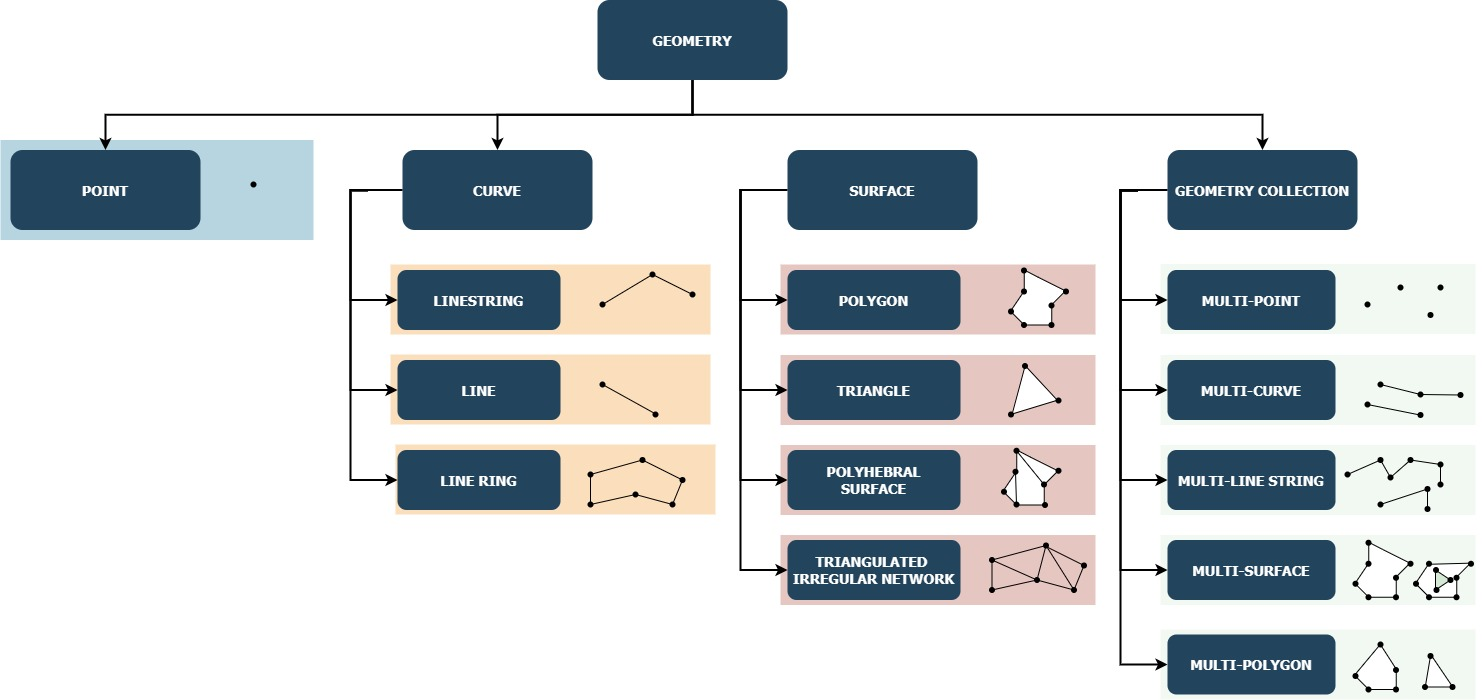
\includegraphics[width=\textwidth]{img/Geometries.jpg}}
    \caption{Classes of geometries in the feature-based model, exemplified by the geometry nearby.}
    \label{fig:example_geometries}
\end{figure}

\subsection{Algebra and Calculi of Qualitative Spatial Relations}\label{II-subsec:algebraCalculi}

Qualitative spatial relations provide a way to describe how spatial features relate to one another without relying on exact measurements. These relations are essential for capturing spatial knowledge in cases where precise quantitative data may not be available or necessary. Qualitative spatial relations can be categorized into various types, with topological relations being one of the most important.

Several algebras and calculi have been developed to formalize and reason about qualitative spatial relations. These formal systems define the rules and operations that can be applied to spatial relations to derive new information. Common calculi include the \acrfull{RCCLabel} and the 9-intersection model (9IM), both of which are widely used for reasoning with topological relations \cite{randellSpatialLogicBased1992}, \cite{egenhoferCategorizingBinaryTopological1991}. These frameworks enable efficient reasoning about how spatial features relate in terms of connectivity, adjacency, containment, and other qualitative properties.

% \paragraph{Region Connection Calculus (RCC)} The RCC is a formalism for representing and reasoning about spatial regions and their relationships. It defines several basic topological relations between regions, such as disconnection, external connection, partial overlap, and containment. This calculus allows for reasoning about how different spatial regions interact and relate to each other.

% \paragraph{9-Intersection Model} The 9-intersection model, proposed by Egenhofer, is another important formalism for spatial reasoning. It uses nine intersections between the boundaries, interiors, and exteriors of two spatial objects to classify their topological relations. The model identifies basic relations such as disjointness, overlap, and containment, among others.

\subsubsection{Topological Relations}\label{II-subsec:topologicalRelations}

Topology is a specialized field within mathematics that builds upon the foundations of geometry and set theory. It focuses on the study of spatial properties, such as space, dimension, and transformation, that remain unchanged under continuous deformation (stretching, twisting, etc.) \cite{janichTopology1984}. This approach is useful in geospatial systems where queries often include topological terms like "crosses" or "borders". For instance, questions such as "Which river crosses the city of Pisa?" or "Which municipalities border the municipality of Florence?" rely on understanding these spatial relationships.

Max Egenhofer made significant strides in this area by developing an algebra of binary topological relations that applied to two-dimensional regions with connected boundaries in ${\rm I\!R}^2$ \cite{egenhoferFormalDefinitionBinary1989}. His key contribution was the \acrfull{4IMLabel}, which categorizes topological relations based on the interactions of boundaries and interiors between two regions. In the 4IM, the classification of relationships is based on the intersections of the boundaries and interiors of two features $A_1$, $A_2$. Each intersection may be empty $(0)$ or nonempty $(\neg 0)$, resulting in a total of $2^4 = 16$ combinations. Each case is represented by a matrix of values:

\begin{equation}
M = 
\begin{pmatrix} 
\partial A_1 \cap \partial A_2 & \partial A_1 \cap A_2^{\circ} \\ 
A_1^{\circ} \cap \partial A_2 & A_1^{\circ} \cap A_2^{\circ} 
\end{pmatrix}
\end{equation}

The interior $A^{\circ}$ of a generic feature $A$ may be defined as:

\begin{equation}
A^{\circ} = A - \partial A,
\end{equation}

where $\partial A$ denotes the boundary of $A$.

Considerating the area/area cases there are 8 possible relationship: disjoint, meet, contains, covers, equal, overlap, inside, and coveredBy showed in figure \ref{fig:4IM}

\begin{figure}[h!tb]
    \centerline {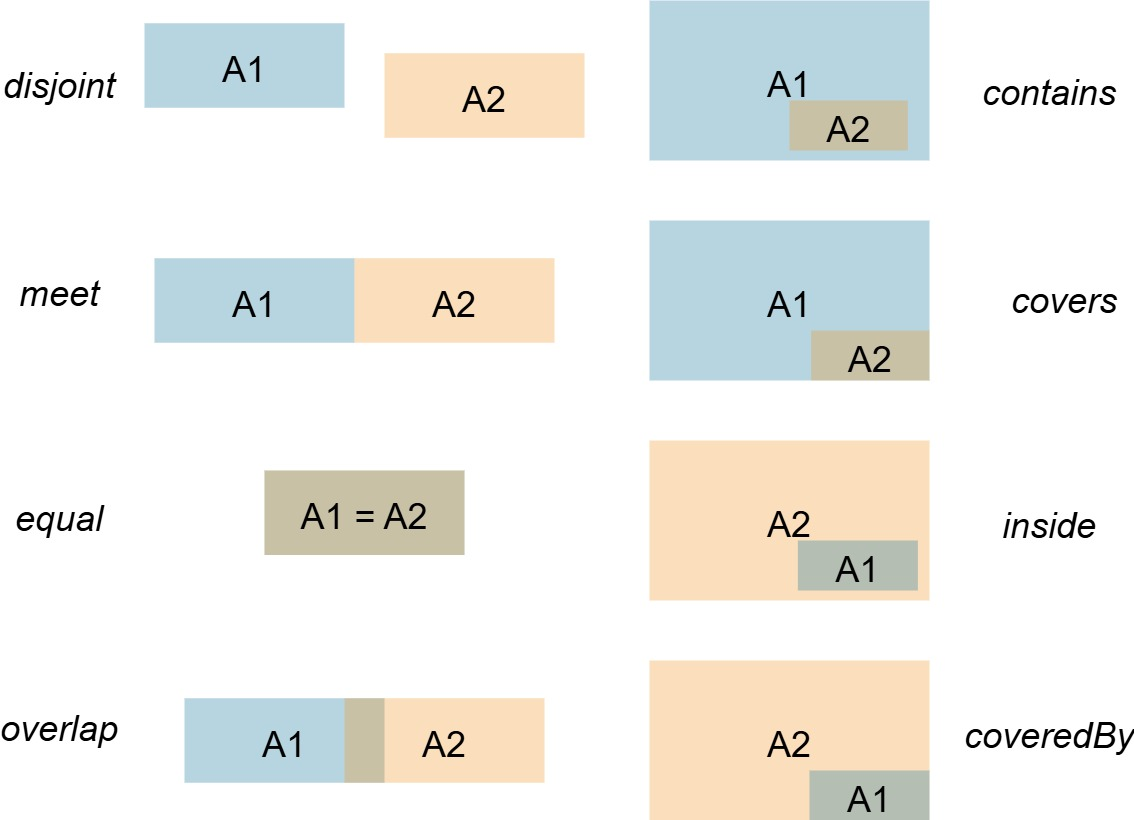
\includegraphics[width=\textwidth]{img/4IM.jpg}}
    \caption{The eight relations area/area of 4IM.}
    \label{fig:4IM}
\end{figure}

Building on the \acrshort{4IMLabel}, Egenhofer and Herring extended this model by incorporating the exterior of the regions, leading to the development of the \acrfull{9IMLabel} \cite{egenhoferCategorizingBinaryTopological1991}. While \acrshort{9IMLabel} provides the same region-to-region relations as the \acrshort{4IMLabel}, it expands the framework to include more detailed interactions between regions, lines, and points, generating a total of 56 \acrshort{JEPDLabel} relations. The \acrshort{9IMLabel} also considers the exterior of features, besides interior and boundary. The exterior $A^{-}$ of a feature $A$ is defined as:

\begin{equation}
A^{-} = \mathbb{R}^2 - A,
\end{equation}

Therefore, it is necessary to consider the following matrix of nine sets:

\begin{equation}
M = 
\begin{pmatrix} 
\partial A_1 \cap \partial A_2 & \partial A_1 \cap A_2^{\circ}  & \partial A_1 \cap A_2^{-} \\ 
A_1^{\circ} \cap \partial A_2 & A_1^{\circ}  \cap A_2^{\circ}  & A_1^{\circ}  \cap A_2^{-} \\
A_1^{-} \cap \partial A_2 & A_1^{-} \cap A_2^{\circ}  & A_1^{-} \cap A_2^{-} 
\end{pmatrix}
\end{equation}


Later, Clementini and his colleagues introduced further enhancements by considering the dimension of each intersection, which resulted in the \acrfull{DE9IMLabel} \cite{clementiniSmallSetFormal1993, clementiniComparisonMethodsRepresenting1995a}. The \acrshort{DE9IMLabel} provides a more nuanced approach by accounting for up to 81 \acrshort{JEPDLabel} binary topological relations. This model uses a 3x3 matrix, where each cell represents the dimensional relationship between different parts of two regions—such as their boundaries, interiors, and exteriors. The matrix's values reflect whether these intersections are empty, of a specific dimension, or simply irrelevant.

The \acrshort{DE9IMLabel} accounts for 81 \acrshort{JEPDLabel} binary topological relations. If we denote  $dim(A)$ the dimension the following 3 × 3 matrix M gives us all these 81 binary topological relations between regions A1 and A2:

\begin{equation}
M = 
\begin{pmatrix} 
dim(\partial A_1 \cap \partial A_2) & dim(\partial A_1 \cap A_2^{\circ}) & dim(\partial A_1 \cap A_2^{-}) \\ 
dim(A_1^{\circ} \cap \partial A_2) & dim(A_1^{\circ}  \cap A_2^{\circ}) & dim(A_1^{\circ} \cap A_2^{-}) \\
dim(A_1^{-} \cap \partial A_2) & dim(A_1^{-} \cap A_2^{\circ}) & dim(A_1^{-} \cap A_2^{-})
\end{pmatrix}
\end{equation}

The cells of \( M \) can take the following values: \( -1 \) (empty intersection), \( 0, 1, 2, T \) (true) = \(\{0, 1, 2\}\), \( F \) (false) = \(\{-1\}\), and \( * \) (don’t care) = \(\{-1, 0, 1, 2\}\).


In parallel, Tony Cohn and his team at the University of Leeds developed the \acrfull{RCCLabel}, which provides another way to describe the spatial relationships between regions \cite{randellSpatialLogicBased1992}. \acrshort{RCCLabel} is centered around the concept of "is connected to" binary predicate. There is a very close correspondence between the relations of 4IM, DE9IM, and RCC-8 captured in table \ref{tab:comparingRCC8_4IM_DE9IM}. However, \acrshort{9IMLabel} and \acrshort{DE9IMLabel} only consider single-piece regions without holes in two-dimensional space while RCC-8 allows much more general regions. This makes reasoning in \acrshort{9IMLabel} and \acrshort{DE9IMLabel} harder than reasoning in \acrshort{RCCLabel} \cite{grigniTopologicalInference1995, renzCanonicalModelRegion2002}.
    

\begin{table}[h!tb]
   \centering \caption{Comparing 4IM, RCC-8, and DE9IM}
   \label{tab:comparingRCC8_4IM_DE9IM}
   \vskip 0.2cm
   %%
   \scalebox{0.90}{
	    %% The {|c|c|c|c|c|} define the number of columns.
	    %% c means centered
	    %% | defines a vertical line between two columns 
	    \begin{tabular}{|c|c|c|}
	      \hline
	      \textbf{4IM} & \textbf{RCC-8} & \textbf{DE9IM}  \\
            \hline
            \textit{equals} & EQ & \textit{equals} \\
            \hline
            \textit{disjoint} & DC & \textit{disjoint} \\
            \hline
            \textit{intersects} & $\neg$ DC & $\neg$ \textit{disjoint} \\
            \hline
            \textit{touches} & EC & \textit{meet} \\
            \hline
	        \textit{within} & (NTPP, TPP) & \textit{(inside, coveredBy)} \\
            \hline
            \textit{contains} & (NTPP-1, TPP-1) & \textit{contains,covers} \\
            \hline
            \textit{overlaps} & PO & \textit{overlap} \\
	      \hline
	      
	    \end{tabular}
	 }
 \end{table}

One challenge in dealing with topological relations is the uncertainty in determining the exact relationship between regions. In such cases, disjunctive expressions, which combine several possible relations, are used to describe what is known. For example, the relationship between two regions A and B might be expressed as a disjunction like $A \left( PO \lor TPP \lor NTPP \right) B$, capturing the possibility of multiple topological configurations.

In some cases, RCC-5, a simplified version of RCC-8, is used. RCC-5 ignores the boundary of regions, thus reducing the number of distinct relations by combining some of the RCC-8 relations. For instance, it merges distinctions like "disconnected" (DC) and "externally connected" (EC) into a single "discrete from" (DR) relation, and simplifies "proper part" (TPP and NTPP) into a single "proper part" (PP) relation.

% \subsubsection{Reasoning with Topological Relations}

% The field of qualitative spatial reasoning and related research in geographic information systems (GIS) and spatial databases has produced a wealth of insights on how to reason using topological relations. Reviews by Cohn and Renz [2008], as well as Renz and Nebel [2007], provide comprehensive overviews of the progress in this area.

% One major problem in this field is determining the consistency of a set of topological statements. For example, given regions A, B, and C, consider the following RCC-8 relations: A is a tangential proper part of B (ANTPPB), B is a tangential proper part of C (BNTPPC), and C is disconnected from A (CDCA). These statements are inconsistent because the relationships between the regions cannot simultaneously hold. Consistency-checking algorithms rely on constraint networks [Dechter 2003, Rossi et al. 2006], which represent spatial relations as constraints between pairs of regions. In an RCC-8 constraint network, nodes represent regions, and edges represent possibly disjunctive relations between them. Techniques like path consistency and efficient backtracking are often employed to resolve these disjunctions [Renz and Nebel 2007].

% Reasoning with disjunctive relations (i.e., where the exact relation is unknown but multiple possibilities are specified) is NP-hard, but research has identified certain tractable subsets of RCC-8 relations [Renz and Nebel 2007]. For example, if the network contains only basic RCC-8 relations (no disjunctions), the consistency problem can be solved in polynomial time using path consistency algorithms [Renz and Nebel 1999]. Unfortunately, the same is not true for DE9IM, where the corresponding problem remains NP-hard [Grigni et al. 1995].

% Another important reasoning task is computing entailments—deriving new relationships based on existing ones. For example, if A is a tangential proper part of B (ANTPPB) and B is a tangential proper part of C (BNTPPC), we can infer that A is a tangential proper part of C (ANTPPC). This is usually done using transitivity tables and constraint propagation methods. Table 2.2 provides an example of such a transitivity table for RCC-8 relations.

% \subsubsection{Cardinal directions} 
% Cardinal direction form another important aspect of qualitative spatial relations. These relations describe how objects are positioned relative to one another using directions like north, south, east, and west. Cardinal direction relations are particularly useful in applications such as navigation, geographic information systems, and spatial querying, where relative orientation is important.

% Cardinal direction relations can be formalized using frameworks such as the \textit{Cardinal Direction Calculus} (CDC) \cite{frank1991}. This calculus captures the relative positions of spatial objects based on the principal directions (north, south, east, west) and often includes intermediate directions (e.g., northeast, southwest). In such a model, a relation between two regions might be expressed as follows: "Region \(A\) is north of Region \(B\)" or "Region \(C\) is to the southeast of Region \(D\)".

% CDC-based reasoning can be applied in spatial databases and GIS for tasks such as retrieving objects located in a particular direction from a reference point or for aligning spatial data based on relative positions. For example, in urban planning, cardinal direction reasoning can be used to plan developments with respect to existing infrastructure, ensuring that new projects are positioned according to specific directional requirements.


\subsection{Representation Techniques}\label{II-subsec:representationTechniques}

The representation of spatial data is a critical aspect \acrshort{GISLabel} and spatial reasoning. Different techniques can be employed depending on the nature of the data and the required level of precision. The most common representation techniques include raster representation, vector representation, and representation by constraints. Each method has its advantages and limitations, depending on the application and type of spatial data.

\subsubsection{Raster Representation}\label{II-subsubsec:raster}
Raster representation uses a grid of equally spaced cells or pixels to represent spatial information. Each cell in the raster grid holds a value that represents some property of the space at that location, such as elevation, temperature, or land cover. Raster data is particularly useful for representing continuous spatial phenomena, such as terrain or satellite imagery.

The resolution of a raster dataset depends on the size of the cells; smaller cells provide higher resolution but require more storage space. This representation is ideal for applications that require the analysis of spatial patterns or gradual changes across a landscape. However, it may not be the most efficient for representing discrete features, such as roads or administrative boundaries, where vector data may be more appropriate \cite{burroughPrinciplesGeographicalInformation1986}.

\subsubsection{Vector Representation}\label{II-subsubsec:vector}
In contrast, vector representation uses geometric shapes—points, lines, and polygons—to represent spatial features. Points can represent discrete locations, such as cities or landmarks, lines are used for linear features like rivers or roads, and polygons represent areas such as administrative boundaries or land parcels.

Vector data is ideal for representing discrete, well-defined features with precise boundaries. It is often preferred in applications that require detailed spatial analysis or where the exact shape and position of features are important. The storage of vector data is generally more efficient than raster data for discrete features, and vector models are widely used in \acrshort{GISLabel} for tasks such as map-making, spatial querying, and network analysis \cite{goodchildGeographicalDataModeling1992}.

\subsubsection{Representation by Constraints}\label{II-subsubsec:constraint}
Representation by constraints is a more abstract method for representing spatial features. Rather than explicitly storing the shape or geometry of a feature, this technique represents spatial objects through a set of constraints or rules that must be satisfied. These constraints may describe spatial relationships, such as proximity, containment, or alignment, between features.

This representation is particularly useful in scenarios where spatial data is incomplete, uncertain, or imprecise. By specifying constraints, it is possible to define the relationships between features without requiring precise geometrical data. This method is often employed in qualitative spatial reasoning, where the goal is to reason about the relationships between spatial objects rather than their exact locations or shapes \cite{clarkeSituationalCrimePrevention1997}.

\subsubsection{Comparison of Representation Techniques}\label{II-subsubsec:comparisonRepresentation}

Each representation technique has its strengths and weaknesses, depending on the nature of the spatial data and the specific application. Raster representation is well-suited for continuous data and large-scale spatial patterns, but it can be inefficient for representing discrete features. Vector representation is highly efficient for discrete features with precise boundaries, but it may not perform as well when dealing with continuous phenomena. Representation by constraints is ideal for reasoning about spatial relationships in the absence of precise data, but it may require more computational effort to derive specific geometric properties.


\section{Semantic Web Technologies}\label{II-sec:semantic_web_technologies}

The Semantic Web extends the current web by enabling sharing and reusing data across applications, enterprises, and communities. It relies on formal knowledge representation to structure data in a machine-readable and interoperable format \cite{berners-leeSemanticWebNew2001}. This section provides a detailed overview of Semantic Web technologies foundational to this research. We explain how the \acrshort{RDFLabel} models data as triples, how the \acrshort{OWLLabel} facilitates complex ontology definitions, and how \acrshort{SPARQLLabel} enables querying of \acrshort{RDFLabel} data.

\subsection{ \acrfull{RDFLabel}}\label{II-subsec:rdf}

The \acrlong{RDFLabel} is a standard model for data interchange on the web \cite{beckettDesignImplementationRedland2002, danbrickleyRDFSchema112014, mcbrideResourceDescriptionFramework2004}. The \acrshort{RDFLabel} framework facilitates the representation of information about resources in graph form. It operates on the principle of articulating statements about resources through subject-predicate-object expressions, commonly referred to as triples. An \acrshort{RDFLabel} triple comprises a subject, the resource being described, a predicate, the property or aspect of the subject, and an object, which can be either another resource or a literal value representing the property's value.

For example, the statement "Sherlock Holmes is an enemy of Dr. Moriarty" can be represented as:

\begin{itemize}
    \item Subject: \texttt{ex:sherlock}
    \item Predicate: \texttt{ex:isEnemyOf}
    \item Object: \texttt{ex:moriarty}
\end{itemize}

This triple can be visualized as a directed graph, where nodes represent resources and edges represent predicates.

\subsubsection{\acrfull{TurtleLabel}}\label{II-subsubsec:turtle}

\acrfull{TurtleLabel} is one of the most common syntaxes for expressing \acrshort{RDFLabel} data. It is a compact, human-readable format that is closely related to \acrshort{SPARQLLabel}, an \acrshort{RDFLabel} query language. Although \acrshort{RDFLabel} can be serialized in various formats, such as \textit{N-Triples}, \textit{JSON-LD}, and \textit{RDF/XML}, \acrshort{TurtleLabel} is preferred in this thesis for its simplicity and readability.

For example, in Turtle, the previous \acrshort{RDFLabel} triple could be written as:
\begin{lstlisting}[caption=Example triple in Turtle with prefixed names, label={lst:prefix-names}]
    ex:sherlock ex:isEnemyOf ex:moriarty
\end{lstlisting}

This concise representation helps developers work with \acrshort{RDFLabel} data more efficiently, especially when dealing with large datasets.

\subsubsection{\acrfullpl{IRILabel}}\label{II-subsubsec:iri}

\acrshort{RDFLabel} uses \acrfullpl{IRILabel} to uniquely identify resources. \acrshortpl{IRILabel} ensure that each resource is globally unique, facilitating data integration from multiple sources. An \acrshort{IRILabel} is a string of characters used to identify resources uniquely. It is an extension of the \acrfull{URILabel}, allowing the inclusion of non-ASCII characters, making it more adaptable to a globalized web. \acrshortpl{IRILabel} can be represented in three primary forms in Turtle:

\begin{itemize}
    \item Absolute \acrshort{IRILabel} represents a complete \acrshort{IRILabel} \\
    \texttt{<http://example.org/sherlock>}.
    \item Relative \acrshort{IRILabel} is a shorter version that refers to a base \acrshort{IRILabel} \\
    \texttt{<sherlock>}.
    \item Prefixed Names combines a prefix and a local name \\
    \texttt{ex:sherlock}. The prefix (e.g., \texttt{ex:}) is defined in the \acrshort{TurtleLabel} document.
\end{itemize}

\subsubsection{Literals and Data Types}\label{II-subsubsec:literals}

Objects in \acrshort{RDFLabel} triples can be literals, which are concrete values such as strings, numbers, or dates. Literals can have data types specified using XML Schema data types \cite{paulv.bironXMLSchemaPart2004}. For instance:

\begin{lstlisting}[caption=Example triple in Turtle with an integer literal, label={lst:integer-literal}]
ex:Paris ex:population "2148327"^^xsd:integer .
\end{lstlisting}

\subsection{\acrfull{RDFSLabel}}\label{II-subsec:rdfs}

\acrfull{RDFSLabel} extends \acrshort{RDFLabel} by providing a basic vocabulary for describing properties and classes of  \acrshort{RDFLabel} resources \cite{danbrickleyRDFSchema112014}. Key elements in \acrshort{RDFSLabel} include Classes, defined using \texttt{rdfs:Class} to represent groups of resources, and Properties, defined using \texttt{rdfs:Propery} to represent relationships between resources. Subclass relationships are specified using \texttt{rdfs:subClassOf}, which establishes class hierarchies. Additionally, Domain and Range are specified using \texttt{rdfs:domain} and \texttt{rdfs:range}, indicating the classes to which a property applies and the type of values it can have.


\subsection{\acrfull{OWLLabel}}\label{II-subsec:owl}

The acrfull{OWLLabel} is designed for representing rich and complex knowledge about things, groups of things, and relations between things \cite{OWLWebOntologya,bechhoferOWLWebOntology2009, OWLWebOntologyb, OWLWebOntologyc}. \acrshort{OWLLabel} builds upon \acrshort{RDFLabel} and \acrshort{RDFSLabel}, offering greater expressiveness for defining ontologies.

The World Wide Web Consortium (W3C) classifies \acrshort{OWLLabel} into three sub languages: \acrshort{OWLLabel} Lite, \acrshort{OWLLabel} DL, and \acrshort{OWLLabel} Full \cite{bechhoferOWLWebOntology2009}.

\begin{itemize}
    \item \acrshort{OWLLabel} Lite is the simplest version of \acrshort{OWLLabel}, providing a basic classification hierarchy and simple constraints. It permits only the expression of relationships with a maximum cardinality of 0 or 1, making it easier to implement. \acrshort{OWLLabel} Lite restricts \acrshort{OWLLabel} DL to a subset of language constructors and lacks certain features such as explicit negation and union. The main disadvantage of \acrshort{OWLLabel} Lite is its limited expressiveness due to these restrictions.
    \item \acrshort{OWLLabel} DL is named for its foundation in Description Logic, a formalism used to represent the relationships between objects and their properties. It offers maximum expressiveness while preserving computational completeness and decidability. This means that any reasoning task will always terminate and provide a correct result. Decidability was a core design criterion for \acrshort{OWLLabel} DL, and many syntactic restrictions are imposed to guarantee this property.
    \item \acrshort{OWLLabel} Full provides the highest level of expressiveness and the syntactic freedom of \acrshort{RDFLabel} but without guarantees on computational complexity. In \acrshort{OWLLabel} Full, computational aspects were not a primary consideration in its design—only logical and semantic aspects were emphasized. Since it does not introduce the syntactic restrictions that \acrshort{OWLLabel} DL uses to retain decidability, reasoning over \acrshort{OWLLabel} Full ontologies can be undecidable, meaning that a reasoner may not always terminate or return a correct result.
\end{itemize}

\subsubsection{Classes, Properties, and Individuals}\label{II-subsubsec:classesProperties}

\acrshort{OWLLabel} allows the definition of three fundamental components: Classes, Properties, and Individuals. Classes represent sets of individuals and serve as categories or types within the ontology. Properties define relationships either between individuals or between individuals and data values, effectively connecting different parts of the ontology. Individuals are the instances of classes, representing the actual objects or entities within the domain of discourse.

\subsubsection{Complex Class Expressions}\label{II-subsubsec:classExpression}

\acrshort{OWLLabel} supports complex class expressions using logical operators such as Intersection, Union, and Complement. The Intersection operator (\texttt{owl
}) defines a class as the intersection of multiple classes, meaning an individual must belong to all specified classes to be a member of this new class. The Union operator (\texttt{owl
}) defines a class as the union of multiple classes, so an individual belonging to any of the specified classes is considered a member of the union class. The Complement operator (\texttt{owl
}) defines a class as the complement of another class, encompassing all individuals that are not members of the specified class.

\subsubsection{Property Characteristics}\label{II-subsubsec:properyCharachteristics}

\acrshort{OWLLabel} allows properties to have specific characteristics, including being Transitive, Symmetric, or Functional. A Transitive property implies that if individual \texttt{A} is related to individual \texttt{B} through this property, and \texttt{B} is related to \texttt{C}, then \texttt{A} is also related to \texttt{C}. A Symmetric property means that if \texttt{A} is related to \texttt{B}, then \texttt{B} is necessarily related to \texttt{A} through the same property. A Functional property is one where each individual can have at most one value for that property, ensuring that the property maps individuals to a single unique value.

\subsubsection{Reasoning and Inference}\label{II-subsubsec:reasoning}

\acrshort{OWLLabel}'s formal semantics enable automated reasoning using description logic reasoners like Pellet \cite{sirinPelletPracticalOWLDL2007}. These reasoners can perform tasks such as Consistency Checking, which involves verifying that the ontology does not contain contradictory information, ensuring logical coherence. They can also perform Classification, determining subclass relationships and organizing the ontology's hierarchy based on defined criteria. Additionally, reasoners handle Instance Checking, determining whether a particular individual is an instance of a specific class by evaluating the individual's properties and relationships against class definitions.

\subsection{\acrfull{SPARQLLabel}}\label{II-subsec:sparql}

\acrshort{SPARQLLabel} plays a pivotal role in querying and manipulating \acrshort{RDFLabel} graphs by using pattern matching techniques \cite{ericprudhommeauxSPARQLQueryLanguage2008}. It enables users to efficiently retrieve, manipulate, and transform data stored in \acrshort{RDFLabel} format, providing powerful capabilities for interacting with structured data on the web.

A typical \acrshort{SPARQLLabel} query comprises several essential components:

\begin{itemize}
    \item \texttt{PREFIX} declarations: These are used to define namespace abbreviations, simplifying the use of long \acrshortpl{URILabel} within the query and making it more readable.
    \item \texttt{SELECT} clause: Specifies the variables to return as part of the query results.
    \item \texttt{WHERE} clause: Contains a set of triple patterns that the query processor matches against the \acrshort{RDFLabel} dataset.
    \item \texttt{FILTER} clause: Applies additional constraints on variables, offering precise control over the query output.
\end{itemize}

Here is an example query that retrieves all cities and their respective populations:

\begin{lstlisting}[caption=Example SPARQL query that retrieves all cities and their population, label={lst:sparql-example}]
PREFIX ex: <http://example.org/> 
SELECT ?city ?population 
WHERE { 
  ?city rdf:type ex:City . 
  ?city ex:hasPopulation ?population . 
} 
\end{lstlisting}

\acrshort{SPARQLLabel} provides a wide range of advanced features to enable more sophisticated data retrieval and analysis:

\begin{itemize}
    \item \textbf{Optional Patterns}: The \texttt{OPTIONAL} keyword is used to include data in the query results if available, without causing the query to fail if that data is missing. This is useful when dealing with incomplete data.
    \item \textbf{Union}: The \texttt{UNION} keyword allows the query to combine multiple patterns, retrieving data that matches any of the specified conditions.
    \item \textbf{Aggregations}: Functions like \texttt{COUNT}, \texttt{SUM}, and \texttt{AVG} are available to perform calculations on the query results, enabling direct data aggregation and analysis within the query itself.
    \item \textbf{Subqueries}: Subqueries allow nesting of queries inside a larger query, breaking down complex data retrieval into manageable components and supporting multi-step data analysis.
\end{itemize}

\subsubsection{\acrshort{SPARQLLabel} Endpoints and Remote Data Access}\label{II-subsubsec:SPARQL}

\acrshort{SPARQLLabel} endpoints serve as interfaces that allow querying \acrshort{RDFLabel} data over the web. These endpoints accept \acrshort{SPARQLLabel} queries via HTTP requests and return results in various formats such as XML, JSON, or CSV. By supporting remote access to \acrshort{RDFLabel} datasets, \acrshort{SPARQLLabel} endpoints facilitate seamless integration of distributed data sources, enabling applications and users to query and analyze data across the web.


\subsection{Data Sharing and Interoperability}\label{II-subsec:data_sharing}

Semantic Web technologies are pivotal for advancing data sharing and interoperability across diverse systems. By adhering to standardized formats, leveraging linked data principles, and reusing established vocabularies, these technologies enable seamless integration of heterogeneous data sources.

\subsubsection{Standardization}\label{II-subsubsec:standardization}

Interoperability is driven by the adoption of universally recognized standards and protocols. The Technologies introduced in the previous sections, such as \acrshort{RDFLabel} \ref{II-subsec:rdf}, \acrshort{OWLLabel} \ref{II-subsec:owl}, and \acrshort{SPARQLLabel} \ref{II-subsec:sparql} provide the necessary structure for consistent data representation and querying across systems. These standards ensure that data can be interpreted and exchanged uniformly, regardless of the system architecture or implementation.

\subsubsection{Linked Data Principles}\label{II-subsubsec:lod}

Tim Berners-Lee’s principles of Linked Data propose a framework for publishing structured data on the web, emphasizing interlinking to create a global data space \cite{timberners-leeLinkedDataDesign2006}. By following these principles, data published on the web can be made accessible, interrelated, and actionable by both humans and machines. This approach fosters a web of interconnected data, enriching information discovery and facilitating broader data integration.

\subsubsection{Vocabulary Reuse}\label{II-subsubsec:vocabularyReuse}

The reuse of existing ontologies and standardized vocabularies is crucial for ensuring semantic consistency and minimizing redundancy. In the forthcoming chapters, we will present a collection of vocabularies and ontologies for reuse. Leveraging these established frameworks improves system compatibility and aligns semantic interpretations.

% \section{Ontology Engineering}\label{sec:ontology_engineering}

% Ontology engineering is the systematic methodology for designing and constructing ontologies, essential for defining shared vocabularies in specific domains. This process emphasizes methodological rigor, efficient reuse of existing ontologies, and the enhancement of both interoperability and operational efficiency. Below, we outline the key stages involved in the ontology development lifecycle, followed by strategies for ontology reuse and a set of best practices.

% \subsection{Ontology Development Lifecycle}

% Ontology development typically progresses through a series of structured stages, each focusing on different aspects of ontology creation and refinement \cite{fernandez-lopezMETHONTOLOGYOntologicalArt1997}:

% \subsubsection{Specification}

% The specification phase defines the ontology's purpose, scope, and requirements. It involves identifying the domain, the intended use cases, and the competency questions that the ontology is expected to address. This stage is critical in ensuring that the ontology is designed with a clear focus and is aligned with the needs of its users.

% \subsubsection{Conceptualization}

% In the conceptualization stage, domain knowledge is organized into a structured format by identifying key concepts, relationships, and constraints. Conceptual models such as taxonomies or class diagrams are often developed at this stage, providing a blueprint for the ontology’s structure.

% \subsubsection{Formalization}

% The formalization stage involves translating the conceptual model into a formal, machine-readable representation using ontology languages such as OWL. This formal representation enables logical inference and automated reasoning, ensuring that the ontology can be computationally processed and interpreted.

% \subsubsection{Implementation}

% Once formalized, the ontology is implemented using tools such as Protégé \cite{musenProtegeProject2015}. This stage involves encoding the ontology’s classes, properties, instances, and axioms. During implementation, the conceptual and formal models are transformed into an operational ontology that can be deployed and queried.

% \subsubsection{Evaluation}

% Evaluation is a critical phase where the ontology is assessed for its correctness, completeness, and consistency. Evaluation methods include validation against the original competency questions and logical consistency checks, often using automated reasoners. Ensuring that the ontology meets the required standards of quality is essential for its effectiveness in real-world applications.

% \subsubsection{Maintenance}

% As the domain evolves, the ontology must be updated to remain relevant. The maintenance phase ensures that the ontology reflects current knowledge, adapts to new requirements, and continues to meet user needs over time. Ongoing refinement and updates are essential to maintain the ontology's accuracy and utility.

% \subsection{Reuse of Existing Ontologies}

% Reusing existing ontologies is a best practice in ontology engineering, as it accelerates development, enhances interoperability, and ensures alignment with established standards. The primary strategies for ontology reuse include:

% \begin{itemize} \item \textbf{Importing}: Incorporating entire ontologies or specific modules from existing ones to leverage their predefined structures and relationships. \item \textbf{Aligning}: Mapping concepts between different ontologies to establish equivalences or hierarchies, facilitating data integration across diverse domains. \item \textbf{Extending}: Enhancing existing ontologies by adding new concepts, properties, or relationships to meet additional requirements while retaining compatibility with established ontologies. \end{itemize}

% \subsection{Best Practices in Ontology Engineering}

% Adopting best practices in ontology engineering ensures the creation of robust, maintainable, and reusable ontologies. Key best practices include:

% \begin{itemize} \item \textbf{Modularity}: Designing ontologies as modular components to enhance reusability, maintainability, and scalability. Modular ontologies allow for easier updates and integration with other ontologies. \item \textbf{Documentation}: Providing comprehensive and clear documentation of the ontology’s structure, purpose, and design decisions. Good documentation is crucial for enabling others to understand, use, and extend the ontology. \item \textbf{Versioning}: Implementing a version control system to manage changes over time, track modifications, and ensure backward compatibility. This practice supports transparency and allows for incremental improvements. \item \textbf{Community Engagement}: Involving domain experts and stakeholders in the development process. Collaborative engagement ensures the ontology reflects expert knowledge and meets community needs, increasing its adoption and relevance. \end{itemize}


\section{Conclusion}\label{II-sec:conclusion}

This chapter laid the theoretical foundation essential for representing geospatial knowledge within narrative structures, integrating principles from narratology, geospatial data modeling, Semantic Web technologies, and ontology engineering. Each of these areas contributes critical tools for the formalization and interpretation of spatiotemporal narratives, facilitating the structured representation of complex geospatial phenomena.

The exploration of narratology provided key insights into the structure and dynamics of narratives, distinguishing between the chronological sequence of events (\textit{fabula}) and their narrative presentation (\textit{syuzhet}). These distinctions are pivotal for understanding both fictional and non-fictional narratives, enabling a nuanced approach to narrative analysis in geospatial contexts. The significance of characters, plots, and narrative structure also emphasized the necessity of defining clear roles and causal relationships within geospatial stories.

Geospatial data modeling, with its focus on the feature-based approach, qualitative spatial relations, and topological reasoning, offered the mathematical and logical tools needed to capture and model spatial relationships within narratives. This approach, combined with effective data representation techniques such as raster and vector models, provides a flexible and precise framework for encoding spatial features in narrative contexts.

Semantic Web technologies, including \acrshort{RDFLabel}, \acrshort{OWLLabel}, and \acrshort{SPARQLLabel}, demonstrated their critical role in enabling interoperability, data integration, and semantic querying, forming the backbone of the formal systems that support geospatial narrative representation. The ability to link data and ensure semantic coherence across multiple domains is crucial for building comprehensive and interoperable geospatial systems.

Finally, the principles of ontology engineering highlighted the importance of methodological rigor, reuse of existing ontologies, and best practices in creating robust, scalable, and maintainable ontologies. This ensures that the formal representation of geospatial narratives is both semantically rich and operationally efficient, allowing for seamless data integration and reasoning across diverse systems.

Together, these theoretical components form a cohesive framework that supports the formal representation and analysis of geospatial narratives, laying the groundwork for further exploration and practical applications in subsequent chapters.

Chapter \ref{chap:overview_narratives} examines the crucial elements of geospatial, spatiotemporal, and narrative representations, providing a detailed overview of the interplay between these domains to facilitate formalized representations of intricate knowledge. Through the exploration of fundamental ontologies pertinent to each field, the pivotal importance of interoperability and reuse is underscored, fostering the seamless integration of data and improved reasoning across various systems.
 

\chapter{An Overview of Geospatial Representation in Narratives}\label{chap:overview_narratives} %Literature Review

\section{Introduction}\label{III-sec:introduction}

After establishing the theoretical framework, we must now examine the state-of-the-art in semantic web technologies and representation techniques for spatiotemporal narratives. In an increasingly data-rich world, the ability to model and interpret spatial and temporal dimensions is essential for understanding complex phenomena and making informed decisions. Ontologies offer a structured framework for capturing and organizing this knowledge, enabling interoperability and facilitating advanced analysis across diverse datasets.

This chapter provides an overview of the ontological frameworks developed to represent geospatial and spatiotemporal knowledge. By analyzing these ontologies, we explore how they formalize key concepts such as location, distance, temporal sequences, and the relationships between spatial entities and events. Understanding these models helps clarify the methodologies used to seamlessly integrate spatial and temporal information.

Building on this foundation, we then examine ontologies designed to represent narratives. Narratives, in this context, are conceived as networks of events interconnected through semantic relations, with each event linked to its components, such as places, participants, and concepts. By exploring narrative ontologies, we investigate how they encapsulate the structural components of stories—events, characters, and plots—and how these elements interact within spatial and temporal contexts. This analysis highlights the mechanisms by which narratives convey meaning and how ontological models can capture the richness and complexity of storytelling.

Through this exploration, we aim to shed light on the intersection between geospatial representation and narrative structures. By integrating ontological approaches from both domains, we enhance our ability to represent, analyze, and interpret complex information systems rich in spatial and temporal dimensions. This integration not only advances theoretical understanding but also has practical implications for fields such as digital storytelling, cultural heritage preservation, bioeconomy studies, and geographic information systems. The insights gained from this chapter underscore the crucial role of ontologies in fostering a comprehensive understanding of narratives enriched with geospatial and spatiotemporal dimensions.

\section{Geospatial Ontologies and Geographic Knowledge}\label{III-sec:geospatialOntologies}

As discussed in chapter \ref{chap:theoretical_framework}, we have explored the concept of an ontology. We now turn our attention to geospatial ontology, which is a structured framework designed to conceptualize geographic knowledge and enable the formal representation of spatial relationships among real-world entities. Like in the geospatial representation, a fundamental element of any geospatial ontology is the "geographic feature" (or simply "feature"), which represents an abstraction of real-world entities \cite{longleyGeographicInformationScience2015}. These features can have both thematic (non-spatial) and spatial characteristics.

As an example, consider the Leaning Tower of Pisa in Italy. As a geographic feature, the tower has various thematic attributes, such as its name (Leaning Tower of Pisa) and its status as part of the UNESCO World Heritage site, Piazza del Duomo. In terms of its spatial characteristics, the tower’s precise location can be quantitatively described using geographic coordinates within the WGS 84 coordinate system, with its longitude and latitude specified as 10.3966 and 43.7229, representing an exact point on the Earth’s surface.

Alternatively, its spatial extent can be described in terms of the land area it occupies, as surveyed by engineers or cartographers. Besides this quantitative description, qualitative spatial information can describe its location relative to other features. For example, the Leaning Tower of Pisa is "southwest of" the Pisa Cathedral and "within" the Piazza del Duomo. Here, "southwest of" represents a cardinal direction relation, while "within" exemplifies a topological relation, illustrating how spatial relationships are captured in qualitative terms.

In the following subsection, we will concentrate on two extensively utilized ontologies: the GeoSPARQL ontology and schema.org, while also providing a brief overview of other geospatial ontologies.

\subsection{The GeoSPARQL Ontology}\label{III-subsec:geosparql}
The GeoSPARQL ontology serves as the foundation for the GeoSPARQL query language, a standard from the \acrfull{OGCLabel} for querying geospatial data represented in \acrshort{RDFLabel} \cite{matthewperryOGCGeoSPARQLGeographic2012}. In the \Cref{chap:evaluation} will be discusses how linked geospatial datasets can be queried using GeoSPARQL, but here we will focus on the structure and design of the GeoSPARQL ontology.

The GeoSPARQL ontology is designed modularly, with components referred to as modules. These modules help organize the ontology efficiently \cite{grauModularReuseOntologies2008}. Although the GeoSPARQL specification refers to it as a "vocabulary"—a set of predefined classes and properties—it extends beyond a simple vocabulary by incorporating taxonomic relationships (subclass and subproperty hierarchies), role typing (defining domains and ranges for properties), and negative constraints (disjointness axioms). Depending on the application’s requirements, GeoSPARQL can be used either as an \acrshort{RDFSLabel} ontology or as an \acrshort{OWLLabel} ontology.

The ontology is structured around three primary components. The first component, called the \textit{Core}, establishes the fundamental vocabulary for spatial objects, serving as the foundational layer of the ontology. Building upon this foundation, the second component, the \textit{Topology Vocabulary Extension}, defines topological relations between spatial objects and their geometries, enhancing the capabilities provided by the core definitions. The third component, the \textit{Geometry Extension}, offers the vocabulary necessary for describing the geometries of spatial objects in detail.

Both the Topology Vocabulary Extension and the Geometry Extension are extensions of the Core component, relying on its basic definitions to function effectively. Additionally, the specification introduces other extensions such as geometry topology, query rewrite, and \acrshort{RDFSLabel} entailment. These supplementary extensions are particularly relevant to the query language aspects of the ontology and are discussed in later chapters.

\subsubsection{Core Component}\label{III-subsubsec:geosparqlCore}

The Core component of the GeoSPARQL ontology introduces the fundamental classes that form the foundation for modeling geospatial information. The two primary classes defined here are \texttt{\gls{geo}SpatialObject} and \texttt{\gls{geo}Feature}.

\texttt{\gls{geo}SpatialObject} is the most general class in the GeoSPARQL ontology, representing any entity that can have a spatial representation. Essentially, any object that has a location or shape in space falls under this class.

\texttt{\gls{geo}Feature} represents geographic features and serves as a superclass for all specific feature classes that users might define in their applications. In the context of geospatial ontologies, a feature could be anything from a mountain to a city or a river.

The relationship between these two classes is established through the subclass mechanism provided by \acrshort{RDFSLabel} and \acrshort{OWLLabel}. Specifically, \texttt{\gls{geo}Feature} is declared as a subclass of \texttt{\gls{geo}SpatialObject}, meaning that every instance of \texttt{\gls{geo}Feature} is also an instance of \texttt{\gls{geo}SpatialObject}.

The formal definitions in Turtle syntax are as follows:

\begin{lstlisting}[caption=Definition of classes \texttt{geo:SpatialObject} and \texttt{geo:Feature} , label={lst:definition-geosparql1}]
/*!\gls{geo}!*/SpatialObject /*!\gls{rdf}!*/type /*!\gls{rdfs}!*/Class, /*!\gls{owl}!*/Class .

/*!\gls{geo}!*/Feature  /*!\gls{rdf}!*/type /*!\gls{rdfs}!*/Class, /*!\gls{owl}!*/Class ;
            /*!\gls{rdfs}!*/subClassOf /*!\gls{geo}!*/SpatialObject .
\end{lstlisting}

\subsubsection{Topology Vocabulary Extension}\label{III-subsubsec:geosparqlTopology}

The Topology Vocabulary Extension provides a set of properties to express topological relationships between spatial objects. It encompasses three families of relations:

First, the Simple Features Relations from the ISO 19125-1 standard \cite{ISO19125120042004}:\\
 \texttt{\gls{geo}sfEquals}, \texttt{\gls{geo}sfDisjoint}, \texttt{\gls{geo}sfIntersects}, \texttt{\gls{geo}sfTouches}, \texttt{\gls{geo}sfCrosses}, \texttt{\gls{geo}sfWithin}, \texttt{\gls{geo}sfContains}, \texttt{\gls{geo}sfOverlaps}.

Second, Egenhofer’s 4-Intersection Model (4IM) Relations, including:\\
\texttt{\gls{geo}ehEquals}, \texttt{\gls{geo}ehDisjoint}, \texttt{\gls{geo}ehMeet}, \texttt{\gls{geo}ehOverlap},\\
\texttt{\gls{geo}ehCovers}, \texttt{\gls{geo}ehCoveredBy}, \texttt{\gls{geo}ehInside}, \texttt{\gls{geo}ehContains}.

Third, the Region Connection Calculus (RCC-8) Relations, like \\
\texttt{\gls{geo}rcc8eq} (equals), \texttt{\gls{geo}rcc8dc} (disconnected), \texttt{\gls{geo}rcc8ec} (externally connected), \texttt{\gls{geo}rcc8po} (partially overlapping), \texttt{\gls{geo}rcc8tppi} (tangential proper part inverse), \texttt{\gls{geo}rcc8tpp} (tangential proper part), \texttt{\gls{geo}rcc8ntpp} (non-tangential proper part), \texttt{\gls{geo}rcc8ntppi} (non-tangential proper part inverse).

An important aspect of these properties is that they are designed to relate any spatial entities, not just geometric objects. Therefore, their domain and range are both defined as \texttt{\gls{geo}SpatialObject}, allowing the relations to be used with features, geometries, or any other spatial entities.

For example, the definition of the property \texttt{\gls{geo}sfDisjoint} is as follows (other properties are defined similarly):

\begin{lstlisting}[caption=Definition of the property \texttt{geo:sfDisjoint} , label={lst:definition-disjoint}]
geo:sfDisjoint rdf:type rdf:Property, owl:ObjectProperty ;
               rdfs:domain geo:SpatialObject ;
               rdfs:range geo:SpatialObject .
\end{lstlisting}

\subsubsection{Geometry Extension}\label{III-subsubsec:geosparqlGeometry}

The Geometry Extension component adds classes, properties, and datatypes specifically for handling geometries. The central class introduced is \texttt{\gls{geo}Geometry}, which represents any geometric object.

Two key aspects of \texttt{\gls{geo}Geometry} are that it is a subclass of \texttt{\gls{geo}Spatial\\Object}, situating it within the hierarchy of spatial entities, and it is declared to be disjoint with \texttt{\gls{geo}Feature}, meaning an instance cannot simultaneously be both a geometry and a feature.

The properties connecting \texttt{\gls{geo}Feature} and \texttt{\gls{geo}Geometry} are \texttt{\gls{geo}has\\Geometry} and \texttt{\gls{geo}hasDefaultGeometry}. The property \texttt{\gls{geo}hasGeometry} associates a feature with one of its geometries; its domain is \texttt{\gls{geo}Feature}, and its range is \texttt{\gls{geo}Geometry}. The property \texttt{\gls{geo}hasDefaultGeometry} is a subproperty of \texttt{\gls{geo}hasGeometry}, used to link a feature to its default geometry, which is the primary geometry used in spatial calculations when no specific geometry is specified.

These properties are formally defined as:

\begin{lstlisting}[caption=Definition of the properties \texttt{geo:hasGeometry} and \texttt{geo:hasDefaultGeometry} , label={lst:definition-hasGeometry}]
geo:hasGeometry rdf:type rdf:Property, owl:ObjectProperty ;
                rdfs:domain geo:Feature ;
                rdfs:range geo:Geometry .

geo:hasDefaultGeometry rdf:type rdf:Property, owl:ObjectProperty ;
                       rdfs:subPropertyOf geo:hasGeometry ;
                       rdfs:domain geo:Feature ;
                       rdfs:range geo:Geometry .
\end{lstlisting}

It is important to note that the GeoSPARQL ontology does not restrict the number of geometries a feature can have (no cardinality constraints are enforced). While the specification treats having multiple geometries for a single feature as a modeling error, users can enforce such constraints using additional tools. For instance, the Shapes Constraint Language (SHACL) can be used to specify constraints like cardinality for users of the \acrshort{RDFSLabel} version \cite{holgerknublauchShapesConstraintLanguage2017}. Alternatively, for users of the \acrshort{OWLLabel} version, declaring properties as functional can enforce that a feature has only one geometry, though this may affect performance.

% Additional properties in the Geometry Extension provide metadata about geometries. These include \texttt{geo:coordinateDimension}, which captures the number of components in coordinate tuples (axes); \texttt{geo:spatialDimension}, capturing the number of spatial components in coordinate tuples; \texttt{geo:dimension}, representing the topological dimension of the geometry; \texttt{geo:isEmpty}, indicating if the geometry is empty; and \texttt{geo:isSimple}, indicating if the geometry is simple (no self-intersections).

% All these properties have \textbf{geo:Geometry} as their domain. The first three have ranges of \textbf{xsd:integer}, and the last two have ranges of \textbf{xsd:boolean}.

% \begin{verbatim}
% geo:coordinateDimension rdf:type rdf:Property, owl:DatatypeProperty ;
%                         rdfs:domain geo:Geometry ;
%                         rdfs:range xsd:integer .

% geo:dimension rdf:type rdf:Property, owl:DatatypeProperty ;
%               rdfs:domain geo:Geometry ;
%               rdfs:range xsd:integer .

% geo:spatialDimension rdf:type rdf:Property, owl:DatatypeProperty ;
%                      rdfs:domain geo:Geometry ;
%                      rdfs:range xsd:integer .

% geo:isEmpty rdf:type rdf:Property, owl:DatatypeProperty ;
%             rdfs:domain geo:Geometry ;
%             rdfs:range xsd:boolean .

% geo:isSimple rdf:type rdf:Property, owl:DatatypeProperty ;
%              rdfs:domain geo:Geometry ;
%              rdfs:range xsd:boolean .
% \end{verbatim}

To represent geometries, GeoSPARQL uses typed literals with the datatypes \texttt{\gls{geo}} \texttt{wktLiteral} and \texttt{\gls{geo}gmlLiteral}, corresponding to \acrfull{WKTLabel}\cite{WellknownTextRepresentationa} and \acrfull{GMLLabel}\cite{GeographyMarkupLanguagea} formats, respectively.

Examples of geometry literals include:

\begin{itemize}
   
 \item  \acrshort{WKTLabel} Literal without specified \acrshort{CRSLabel} (defaults to WGS 84):

\begin{lstlisting}[caption=WKT literal without CRS, label={lst:wktLiteral}]
    "POINT(-83.38 33.95)"^^geo:wktLiteral
\end{lstlisting}


 \item  \acrshort{WKTLabel} Literal with specified \acrshort{CRSLabel}:

\begin{lstlisting}[caption=WKT literal with CRS specified, label={lst:wktLiteralCRS}]
    "<http://www.opengis.net/def/crs/EPSG/0/4326> POINT(33.95 -83.38)"^^geo:wktLiteral
\end{lstlisting}

The \acrshort{IRILabel} <http://www.opengis.net/def/crs/EPSG/0/4326> represents the World Geodetic System 1984 (WGS 84).

 \item  \acrshort{GMLLabel} Literal:

\begin{lstlisting}[caption=GML literal, label={lst:GMLLiteral}]
"<gml:Point srsName=\"http://www.opengis.net/def/crs/OGC/1.3/CRS84\" xmlns:gml=\"http://www.opengis.net/gml\">
  <gml:pos>-83.38 33.95</gml:pos>
</gml:Point>"^^geo:gmlLiteral
\end{lstlisting}

\end{itemize}

Properties for geometry serialization are \texttt{\gls{geo}hasSerialization}, which links a geometry to its serialized form (untyped literal); \texttt{\gls{geo}asWKT}, a subproperty of \texttt{\gls{geo}hasSerialization} that links a geometry to its WKT serialization; and \texttt{\gls{geo}\\asGML}, also a subproperty of \texttt{\gls{geo}hasSerialization}, linking a geometry to its GML serialization.

% \subsection{The Schema.org Ontology}

% In the realm of the Web, Schema.org stands out as a significant geospatial ontology. It is a collaborative community initiative with the mission to create, maintain, and promote schemas for structured data on the Web. By providing a collection of shared vocabularies, Schema.org enables webmasters to annotate their web pages with semantic information. This semantic enrichment facilitates major search engines (like Google and Bing) in better understanding and efficiently indexing web content.

% From a modeling standpoint, Schema.org offers users an extensive taxonomy comprising 598 classes. Each class is associated with a set of properties, totaling 862 properties, whose domains and ranges can generally be a union of classes. This level of expressiveness surpasses the capabilities of \acrshort{RDFSLabel}, which cannot model such property ranges, but fits well within the expressive power of OWL (Web Ontology Language) \cite{OWLWebOntologya}.

% Specifically for geospatial modeling, Schema.org provides three main classes: \texttt{schema:GeoCoordinates}, \texttt{schema:GeoShape}, and \texttt{schema:Place}. The class \texttt{schema:GeoCoordinates} is used to represent the coordinates of a place considered as a point, possibly including elevation. The class \texttt{schema:GeoShape} allows encoding the geometric shape of a place using lines, rectangles, circles, or polygons. Lastly, \texttt{schema:Place} is intended for modeling entities with a physical extension, such as the Athens airport. In the following sections, these classes and their associated properties are discussed in detail.

% \subsubsection{Class \texttt{schema:GeoCoordinates}}

% The class \texttt{schema:GeoCoordinates} is provided by Schema.org for representing the geographic coordinates of a place when considered as a point, possibly accompanied by elevation information. To capture these details, Schema.org defines the properties \texttt{schema:latitude}, \texttt{schema:longitude}, and \texttt{schema:elevation}, which represent the measurements for latitude, longitude, and elevation, respectively. These measurements are expected to be relative to the WGS 84 coordinate system and are provided as literals of either type \texttt{schema:Number} or \texttt{schema:Text}.

% Except for \texttt{schema:elevation}, which is also defined for \texttt{schema:GeoShape}, the properties \texttt{schema:latitude} and \texttt{schema:longitude} are exclusively used with the class \texttt{schema:GeoCoordinates}. Additionally, instances of \texttt{schema:GeoCoordinates} may include metadata such as the country, address, and postal code associated with the geographic coordinates. These metadata are represented using appropriate properties, which are not detailed here but can be explored further at \url{https://schema.org/GeoCoordinates}.

% The OWL definitions for the class \texttt{schema:GeoCoordinates} and its spatial properties are provided using the Manchester OWL syntax \cite{OWLWebOntologyb}. This syntax is particularly useful for defining property ranges in Schema.org, which may take values belonging to a union of classes. The class \texttt{schema:GeoCoordinates} is defined as a subclass of \texttt{schema:StructuredValue}, a class employed in Schema.org when there is a need to represent property values with complex structures.


% \subsubsection{Class \texttt{schema:GeoShape}}

% The class \texttt{schema:GeoShape} is offered by Schema.org for asserting the geographic shape of a place. The supported shapes include lines, rectangles, circles, and polygons, which correspond to the classes of geometries introduced earlier. To represent these shapes, Schema.org defines the properties \texttt{schema:line}, \texttt{schema:box}, \texttt{schema:circle}, and \texttt{schema:polygon}, respectively, each taking literal values of type \texttt{schema:Text}.

% The modeling of these geometries and their textual representation assumes that coordinates are interpreted in WGS 84, with point geometries encoded by listing their longitude and latitude measurements in that specific order, separated by a comma. A line is a point-to-point path consisting of two or more points, expressed as a series of point objects separated by spaces. A box represents the area enclosed by the rectangle formed by two points—the first point being the lower corner and the second point the upper corner—and is expressed as two points separated by a space. A circle denotes a circular region of a specified radius centered at a specified latitude and longitude, expressed as a pair followed by a radius in meters. A polygon is the area enclosed by a point-to-point path where the starting and ending points are the same, expressed as a series of four or more space-delimited points with identical first and final points.

% It is important to note that \texttt{schema:GeoShape} does not support properties for geometry collections such as multi-line strings or multi-polygons, as discussed in Section 2.1.1. This limitation is significant because many geographic features have such geometries. For example, multi-polygons are used to encode the geometries of administrative divisions of Greece in the GADM dataset, which is presented in Section 6.1 of the next chapter.

% The shapes supported by \texttt{schema:GeoShape} can also include elevation through the property \texttt{schema:elevation}. Elevation measurements are again interpreted in WGS 84 and encoded as literals of type either \texttt{schema:Number} or \texttt{schema:Text}. Similar to \texttt{schema:GeoCoordinates}, instances of \texttt{schema:GeoShape} may carry metadata such as country, address, and postal code associated with the shape. These can be explored further at \url{https://schema.org/GeoShape}.

% The OWL definitions for the class \texttt{schema:GeoShape} and its spatial properties are as follows:


% Before concluding the discussion on \texttt{schema:GeoShape}, it is essential to mention its subclass, \texttt{schema:GeoCircle}. This class is used to represent features occupying a circular geographic area defined by a center and a radius. \texttt{schema:GeoCircle} provides the properties \texttt{schema:geoMidpoint} and \texttt{schema:geoRadius} to represent the center and radius of circles, respectively. The center is specified as an instance of \texttt{schema:GeoCoordinates}, while the radius is given as a literal of type \texttt{schema:Number}, \texttt{schema:Text}, or \texttt{schema:Distance}. Values of the latter type must conform to the form ``\textless Number\textgreater\ \textless SPACE\textgreater\ \textless Unit of measure\textgreater,'' for example, ``10 ft.'' Values for \texttt{schema:geoRadius} are interpreted in meters unless they are literals of type \texttt{schema:Distance}, in which case the unit of measure is obtained directly from the specified value.


% It is worth noting that Schema.org provides two methods for representing circular regions: by asserting them as instances of \texttt{schema:GeoShape} and populating the property \texttt{schema:circle}, or by asserting them as instances of \texttt{schema:GeoCircle}. The latter approach was introduced later to meet publishers' needs for controlling the unit of measure in which the radius is interpreted.

% \subsubsection{Class \texttt{schema:Place}}

% The class \texttt{schema:Place} is used by Schema.org to model entities that have a physical extension. As such, it is a subclass of \texttt{schema:Thing}, the top-level class that every other class in Schema.org specializes, either directly or indirectly. Among the extensive set of metadata properties provided for places—which are not detailed here for brevity—Schema.org includes the geospatial properties \texttt{schema:geo}, \texttt{schema:containsPlace}, and \texttt{schema:containedInPlace}.

% The property \texttt{schema:geo} associates a place with a geometry by relating instances of \texttt{schema:Place} with instances of either \texttt{schema:GeoCoordinates} or \texttt{schema:GeoShape}. The properties \texttt{schema:containsPlace} and \texttt{schema:containedInPlace} correspond to the topological relation of containment and its inverse, respectively, and relate instances of \texttt{schema:Place}.

% It is important to highlight that Schema.org does not specify the underlying topological model for these relations. As discussed in Chapter 2, the choice of topological model is crucial for the interpretation of topological relations and can lead to different formalisms, such as the 4-Intersection Model (4IM), Dimensionally Extended 9-Intersection Model (DE-9IM), or Region Connection Calculus (RCC-8). In a pending extension, Schema.org plans to address this ambiguity by explicitly adopting the DE-9IM model and including the set of properties that accompany it. Currently, these properties are planned to be defined on \texttt{schema:Place} and on a pending superclass of \texttt{schema:GeoShape} called \texttt{GeospatialGeometry}. Interested readers are referred to \url{https://pending.schema.org/GeospatialGeometry} for further information.

% Finally, it is worth mentioning that Schema.org provides a very broad set of subclasses under \texttt{schema:Place}. These include useful classes for representing administrative areas (e.g., cities, states), land formations (e.g., mountains, lakes), civic structures (e.g., bridges, airports, hospitals), and more. All such classes inherit the spatial properties defined for \texttt{schema:Place} and may extend the corresponding set of metadata properties. Readers can explore the full range of these subclasses at \url{https://schema.org/docs/full.html}.

\subsection{The Schema.org Ontology}\label{III-subsec:schemaOrg}

Schema.org is a prominent ontology widely used to structure data on the Web. It is a collaborative initiative aimed at creating and promoting schemas for semantic annotations, which enhance how search engines like Google and Bing index and understand web content. Schema.org provides a large taxonomy consisting of 598 classes and 862 properties, offering significant expressiveness, particularly in geospatial modeling, aligning with the capabilities of \acrshort{OWLLabel} while exceeding the expressiveness of \acrshort{RDFSLabel}.

For geospatial purposes, Schema.org introduces three main classes: \texttt{\gls{schema}\\GeoCoordinates}, \texttt{\gls{schema}GeoShape}, and \texttt{\gls{schema}Place}. \texttt{\gls{schema}GeoCoordinates} is used to represent a geographic point, offering properties such as \texttt{\gls{schema}latitude}, \texttt{\gls{schema}longitude}, and \texttt{\gls{schema}elevation}. These properties are generally associated with the WGS 84 coordinate system and can be expressed as either numbers or text. Latitude and longitude are specific to \texttt{\gls{schema}GeoCoordinates}, while elevation is also used by \texttt{\gls{schema}GeoShape}. Metadata such as country, address, and postal code can also be associated with geographic coordinates.

\texttt{\gls{schema}GeoShape} is used to describe geographic shapes, including lines, rectangles, circles, and polygons. It provides properties like \texttt{\gls{schema}line}, \texttt{\gls{schema}\\box}, \texttt{\gls{schema}circle}, and \texttt{\gls{schema}polygon}, where the coordinates are expressed in WGS 84. Lines are represented as a series of points, rectangles are defined by two corner points, circles are specified by a center and a radius, and polygons are represented as a closed series of points. However, \texttt{\gls{schema}GeoShape} does not support complex geometries like multi-polygons or multi-line strings, which is a limitation when modeling geographic features such as administrative boundaries. Elevation can also be included using the \texttt{\gls{schema}elevation} property. Additionally, \texttt{\gls{schema}GeoCircle}, a subclass of \texttt{\gls{schema}GeoShape}, models circular regions with a center point and a radius, offering flexibility in representing circular areas.

\texttt{\gls{schema}Place} is used to represent entities with a physical extension and is a subclass of \texttt{\gls{schema}Thing}, the root class of Schema.org. Key geospatial properties include \texttt{\gls{schema}geo}, which links a place to its geographic coordinates or shape, as well as \texttt{\gls{schema}containsPlace} and \texttt{\gls{schema}containedInPlace}, which model containment relationships between places. However, Schema.org does not explicitly define a topological model for these relations, which can lead to different interpretations. A future extension aims to incorporate the DE-9IM model to clarify topological relations in \texttt{\gls{schema}Place} and a new class, \texttt{GeospatialGeometry}. 

Schema.org also offers a wide range of subclasses for \texttt{\gls{schema}Place}, covering administrative areas (such as cities and states), natural features (like mountains and lakes), and civic structures (e.g., airports, bridges). These subclasses inherit the geospatial properties of \texttt{\gls{schema}Place} and may include additional metadata. 


\subsection{Other Geosptial Ontologies}\label{III-subsec:otherGeospatialOntologies}

Beyond the well-known geospatial ontologies like GeoSPARQL, several other vocabularies have been developed to represent and share spatial information on the web effectively. These ontologies aim to address specific limitations of existing standards and enhance the expressiveness and interoperability of geospatial data.

The W3C Basic Geo Vocabulary, introduced in 2003 \cite{danbrickleyW3CBasicGeo2003}, provides a foundational \acrshort{RDFLabel} schema for representing geographic points using the World Geodetic System 1984 (WGS84) as a reference datum. It defines a class \texttt{Point} with properties such as \texttt{lat} (latitude), \texttt{long} (longitude), and \texttt{alt} (altitude) to describe point locations. Latitude and longitude are expressed in decimal degrees, while altitude is given in decimal meters above the local reference ellipsoid.

While this vocabulary is widely used for encoding WGS84 coordinates, it has notable limitations. It lacks the ability to represent geometric shapes beyond simple points, such as the borders of countries. Additionally, it does not support the specification of different datums and coordinate systems, which led to its exclusion from more comprehensive standards like GeoSPARQL. Nevertheless, data encoded with the W3C Basic Geo Vocabulary can be converted into GeoSPARQL representations without significant difficulty.

To overcome these limitations, extensions such as GeoRSS \cite{reedOGCGeoRSSEncoding2017} and GeoJSON \cite{butlerGeoJSONFormat2016} were developed. GeoRSS is designed to extend RSS feeds with geographic information, allowing for the encoding of more complex geometries like lines, rectangles, and polygons. It facilitates applications in requesting, aggregating, sharing, and mapping geographically tagged data. GeoJSON, on the other hand, is a geospatial data interchange format based on JSON, capable of encoding various shapes including points and polygons, thus providing a flexible and lightweight means of sharing spatial data.

Recognizing the need for a more expressive vocabulary, the W3C Geospatial Incubator Group proposed updates to the W3C Basic Geo Vocabulary \cite{joshualiebermanW3CGeospatialVocabulary2017}. The aim was to incorporate features from the GeoRSS model, enabling the description of points, lines, rectangles, and polygon geometries along with their associated features, thereby enhancing the vocabulary's utility for representing complex spatial data.

Another significant contribution is the NeoGeo vocabulary developed by Salas and Harth \cite{salasNeoGeoVocabularyDefining2011a}. By analyzing existing geospatial datasets, they identified common patterns and distilled a core set of classes and properties to support typical geometric objects such as points, lines, polygons, and their collections. NeoGeo represents all elements as \acrshort{RDFLabel} resources, maximizing expressiveness. For example, a polygon is represented as an \acrshort{RDFLabel} collection of point resources, allowing detailed geometric descriptions within the \acrshort{RDFLabel} framework. The vocabulary also includes topological relations based on the Region Connection Calculus (RCC-8), providing properties to express spatial relationships between features.

In a different approach, Brodt et al. \cite{brodtDeepIntegrationSpatial2010} proposed representing spatial features in \acrshort{RDFLabel} using spatial literals. These literals contain geometries expressed in the \acrshort{WKTLabel} format, standardized by the OpenGIS Simple Features Specification. The literals are typed to indicate they represent spatial features, enabling their processing as geometric data rather than ordinary strings. While this method embeds all geographic information within a single \acrshort{RDFLabel} statement, it does not assign unique identifiers to individual spatial features, which limits direct referencing and metadata augmentation.

GeoRDF emerged as an RDF-compatible profile intended to represent geographic information such as points, lines, and polygons. It offers both simple and complex profiles for encoding geometries. The simple profile uses comma-separated lists of coordinate pairs to describe lines and polygons, while the complex profile employs \acrshort{RDFLabel} sequences of points. This dual approach allows users to choose the level of complexity that best suits their needs, facilitating flexibility in geometric representations.

Addressing the issue of incomplete geospatial information, Nikolaou and Koubarakis introduced RDF$^i$ \cite{nikolaouQueryingIncompleteInformation2016a}, an extension of \acrshort{RDFLabel} that enables the representation and querying of unknown or partially known property values. RDF$^i$ allows for the use of existential literals in the object positions of triples, indicating the existence of a value without specifying it explicitly. This framework enhances the expressiveness of \acrshort{RDFLabel} in geospatial contexts by accommodating incomplete information, which is common in real-world data scenarios.

Collectively, these ontologies and vocabularies contribute to the evolving landscape of geospatial data representation on the web. By addressing specific needs—such as supporting complex geometries, handling incomplete information, and integrating various data formats—they enhance the capacity to model, share, and query spatial information within the Semantic Web framework. Their development reflects ongoing efforts to create more comprehensive and flexible tools for geospatial data, ultimately facilitating better data interoperability and more powerful spatial analyses.

\section{Spatiotemporal Ontologies}\label{III-sec:spatiotemporal}

Spatiotemporal ontologies integrate both spatial and temporal dimensions in data modeling. While spatial \acrshort{RDFLabel} data management has been extensively researched, many applications require not only spatial information but also a temporal context. Geospatial objects are complex, consisting of multiple interrelated parts, and this complexity increases when the temporal dimension is introduced. As a result, significant research interest has emerged around \acrshort{RDFLabel}-based techniques for managing spatiotemporal data.

\subsection{stRDF: A Spatio-temporal RDF Model}\label{III-subsec:strdf}

During the development of GeoSPARQL by the Open Geospatial Consortium (OGC), Koubarakis et al. \cite{koubarakisModelingQueryingMetadata2010a} independently introduced the stRDF model and the stSPARQL query language. stRDF extends \acrshort{RDFLabel} to support the representation of geospatial data that evolves over time. Similar to GeoSPARQL, stRDF uses two core spatial data types: \texttt{\gls{strdf}WKT} (Well-Known Text) and \texttt{\gls{strdf}GML} (Geography Markup Language), which represent geometries in their respective formats. The property \texttt{\gls{strdf}has\\Geometry} allows users to link features to their geometries without requiring a high-level spatial ontology, unlike GeoSPARQL, which connects geometries through intermediate \acrshortpl{IRILabel}. stRDF directly associates geometry literals with features, providing a simpler but less flexible model.

Koubarakis and Kyzirakos further developed stRDF as a constraint-based \acrshort{RDFLabel} extension to represent both spatial and temporal data. The model is based on the principles of constraint databases and represents spatial and temporal objects using quantifier-free formulas in first-order logic of linear constraints. A first-order language \( L \) is defined to include linear constraints over the rational numbers \( Q \), and semi-linear subsets of \( Q^k \) are used to model geometries. These can capture a variety of spatial shapes, including points, lines, and polygons. However, stRDF does not support complex geometries like circles, which require higher-degree polynomials.

To handle spatial data, stRDF introduces the notion of spatial RDF (sRDF), where triples consist of subjects, predicates, and objects, where objects can be quantifier-free formulas representing spatial data. An example of this approach would be modeling the Tower Of Pisa location as a conjunction of linear constraints:
\begin{lstlisting}[caption=the Tower of Pisa location as a conjunction of linear constraints, label={lst:tower-Pisa-location}]
ex:PisaTower rdf:type ex:LeaningTower;
            ex:hasLocation "x=10 and y=20"^^strdf:SemiLinearPointSet.
\end{lstlisting}
In this example, the location is expressed using the datatype \texttt{\gls{strdf}SemiLinear\\PointSet}, which defines spatial literals as Boolean combinations of linear constraints in \( Q^2 \).

stRDF extends sRDF to include the temporal dimension, enabling the representation of both spatial and thematic data with a temporal component. The temporal constraints are expressed using quantifier-free formulas over rational numbers, where atomic temporal constraints take the form \( x \sim c \), where \( x \) is a variable, \( c \) is a rational number, and \( \sim \) represents a comparison operator. Each stRDF quad has a temporal component \( \tau \), which specifies the time points at which the triple is valid. For example:
\begin{lstlisting}[caption=the Tower of Pisa sensor controle the slope, label={lst:tower-Pisa-slope}]
ex:sensor1 rdf:type ex:Sensor
ex:sensor1 ex:slopeControl "35"^^xsd:decimal at "2024-10-10T00:01:00"^^xsd:dateTime.
\end{lstlisting}
This illustrates how a sensor reading can be annotated with a temporal validity period.

In later work, Koubarakis et al. \cite{koubarakisChallengesQualitativeSpatial2011} introduced stRDFi, a more practical version of stRDF, which replaces linear constraints with OGC standards such as WKT and GML for representing geometries. The stRDFi model allows incomplete spatial information to be represented and queried using qualitative spatial relations. Temporal data is managed using XML Schema datatypes, such as \texttt{xsd:dateTime}, \texttt{xsd:date}, and others. 

\subsection{stSPARQL: A Query Language for Spatio-temporal Data}\label{III-subsec:stsparql}

While GeoSPARQL offers a robust framework for querying spatial data, stRDF required a specialized query language to handle both spatial and temporal dimensions. stSPARQL, introduced by Koubarakis and Kyzirakos, is an extension of \acrshort{SPARQLLabel} that allows querying spatiotemporal data in stRDF. stSPARQL adds spatial and temporal variables to basic graph patterns, enabling advanced spatiotemporal querying. 

Spatial variables in stSPARQL are used to refer to spatial literals such as semi-linear point sets and can be utilized in spatial filters. These filters allow for the comparison of spatial terms using predicates like "inside" or "overlaps". For example, a query might filter results where one geometry is inside another:
\begin{lstlisting}[caption=Filter command with inside predicate, label={lstfilter-inside}]
    filter(?GEO1 inside ?GEO2)
\end{lstlisting}


In addition to spatial variables, stSPARQL introduces temporal variables, which refer to temporal literals or constants. These allow for the querying of temporal data using predicates based on Allen's interval algebra, as demonstrated by a filter expression querying for a temporal event:
\begin{lstlisting}[caption=Filter command with contains predicate, label={lstfilter-inside}]
filter(?T contains "2024-01-01"^^xsd:dateTime)
\end{lstlisting}

stSPARQL also supports advanced spatial functions, such as \texttt{\gls{strdf}union} and \texttt{\gls{strdf}area}, which are not currently available in GeoSPARQL but are planned for future versions. stSPARQLi, an enhanced version of stSPARQL, integrates additional functions from the OGC Simple Features Access standard, allowing users to perform more complex spatial queries. For instance, the \texttt{srdf:Contains} function can check whether one geometry contains another:
\begin{lstlisting}[caption=strdf function Contains in stSPARQL, label={lstfilter-inside}]
srdf:Contains(?GEO, "POINT(669062 4238286); urn:epsg:ggrs87"^^srdf:geometry)
\end{lstlisting}
These spatial functions can also be used in the \texttt{SELECT} part of a query to return derived spatial information, such as the buffer of a geometry.

The Strabon 3.0 system \cite{krr&ateamStrabon}, an open-source platform, implements stSPARQLi and supports querying spatiotemporal data stored in a PostGIS-enabled\cite{PostGIS} \acrshort{RDFLabel} store. Strabon is based on the Sesame \acrshort{RDFLabel} store and extends it with modules for handling spatiotemporal data, including a storage manager and a query engine optimized for spatial queries.

\subsection{Other Spatiotemporal Representation Models}\label{III-subsec:otherSpatiotemporal}

In addition to stRDF and stSPARQL, other models have been developed to handle spatiotemporal data. The STT (Spatial, Temporal, Thematic) framework by Sheth and Perry \cite{perryFrameworkSupportSpatial2008} provides an alternative approach for processing Semantic Web data. This model uses temporal \acrshort{RDFLabel} graphs to represent facts with time intervals, and it introduces an upper-level ontology that distinguishes between continuants (persistent entities) and occurrents (events and processes). The temporal \acrshort{RDFLabel} graphs are used to model discrete time points, allowing for temporal queries.

The gst-Store system, developed by Wang et al. \cite{wangGstStoreEngineLarge2014}, extends \acrshort{RDFLabel} triples to include spatial and temporal features. Each statement is modeled as a five-tuple \( (s, p, o, l, t) \), where \( l \) and \( t \) represent the location and time interval, respectively. The system uses longitude and latitude to represent spatial coordinates and stores temporal information as date intervals.

YAGO2 \cite{hoffartYAGO2SpatiallyTemporally2013a}, an extension of the YAGO knowledge base, incorporates spatiotemporal knowledge using SPOTL tuples (Subject, Predicate, Object, Time, Location). YAGO2 introduces a new class, \texttt{yagoGeoEntity}, to group entities with a permanent location, and uses geographical coordinates to represent these entities' positions. Temporal data in YAGO2 is handled through the \texttt{yagoDate} datatype, which supports dates with varying resolutions, from days to years.

Finally, stRDFS, proposed by Zhu et al. \cite{zhuStRDFSSpatiotemporalKnowledge2020}, extends \acrshort{RDFLabel} with spatiotemporal labels on predicates. This model supports spatiotemporal classes and relations, such as \texttt{Inside}, \texttt{Contains}, and \texttt{Before}, enabling reasoning over spatiotemporal graphs. stRDFS also defines a set of graph algebra operations, such as union, intersection, and difference, allowing users to manipulate spatiotemporal \acrshort{RDFLabel} graphs.

\section{An Ontology for Narratives}\label{III-sec:nont}

The Narrative Ontology (NOnt) \cite{meghiniRepresentingNarrativesDigital2021} is a conceptual framework developed to formalize the representation and modeling of narratives. Narratives, conveyed through various media such as text, images, and videos, are fundamental to human knowledge and cultural heritage. NOnt provides a structured means to digitally represent these narratives, making them accessible for machine processing and enabling tasks like discovery, comparison, and generation in digital environments, such as digital libraries.

At the core of NOnt is the distinction between three main narrative components: Fabula, Narration, and Plot. Fabula refers to the sequence of events in chronological order, representing the story as it ``actually'' occurred, irrespective of whether it is factual or fictional. Narration focuses on the medium or expressive form used to present the fabula, such as a novel, film, or digital media, and how it is portrayed from a particular perspective. Plot (also known as Syuzhet) represents the structured presentation of the fabula, which may involve a reordering of events for thematic or stylistic reasons.

NOnt formalizes these components by detaching narratives from their specific media representations and treating them as structured data. This allows for machine-based analysis, comparison, and synthesis, distinguishing NOnt from traditional digital libraries, which primarily catalog media objects without addressing the underlying narrative content.

The NOnt framework builds upon established ontologies, such as the CIDOC Conceptual Reference Model (CRM) \cite{doerrCIDOCConceptualReference2007a}, FRBRoo \cite{doerrFRBROOCONCEPTUALMODEL2008}, and \acrshort{OWLLabel} Time \cite{TimeOntologyOWL}. Leveraging these ontologies enables the formal representation of narratives while maintaining structured connections to cultural and bibliographic resources. Furthermore, the integration of the Semantic Web Rule Language (SWRL) facilitates the formalization of complex narrative structures through the specification of axioms.

This formalization enhances functionality in digital libraries. Users, such as historians or environmental scientists, can explore, create, and compare narratives to investigate cultural or scientific phenomena in greater depth. For instance, a historian might use NOnt to reconstruct and analyze the sequence of events leading up to a significant historical event, while an environmental scientist could model and compare narratives of environmental changes over time to identify causal relationships. NOnt transforms interactions with narratives, enriching the understanding and exploration of human knowledge through digital ecosystems.

The following sections provide an overview of the foundational ontologies that underpin NOnt, as well as details about its implementation, leading to the development of NOnt+S, an extended version of the base ontology.


\subsection{CIDOC-CRM}\label{III-subsec:cidoccrm}

The CIDOC Conceptual Reference Model (CRM)\cite{doerrCIDOCConceptualReference2007a} is a formal ontology designed to facilitate the integration and exchange of heterogeneous cultural heritage information. Developed by the International Committee for Documentation (CIDOC) under the International Council of Museums (ICOM), CIDOC-CRM enables semantic interoperability across domains like archaeology, social history, and museum documentation. Since 9/12/2006, it is the official standard ISO 21127:2006 \cite{ISO211272023}.

CRM organizes knowledge using \textit{classes} and \textit{properties}. Classes represent categories of entities, such as people, events, and places, while properties define the relationships between these entities, such as \textit{is identified by} or \textit{occurred at}. For instance, a \textit{Person} can be linked to an \textit{Event} through properties like \textit{is identified by} or \textit{occurred at}. This structured representation ensures consistent data exchange across institutions, preserving meaning and enabling cross-disciplinary research.

The CRM's event-centric approach is crucial because it emphasizes historical processes and interactions over time. This focus on events, rather than static objects, allows cultural heritage institutions to represent the dynamic nature of history more effectively, capturing the context in which artifacts, people, and places interact. Furthermore, CIDOC-CRM explicitly models not just tangible heritage, such as artifacts and monuments, but also intangible aspects, such as knowledge, cultural practices, and collective memory. By capturing these intangible elements, CIDOC-CRM allows for a richer and more nuanced understanding of cultural heritage.

CRM is implemented in various formats, such as \acrshort{RDFLabel} and \acrshort{OWLLabel}, making it versatile and adaptable to different system requirements. Its flexible structure and scalability also allow for domain-specific extensions while maintaining a universally applicable core model. For example, the CRM has been extended through CRMinf\cite{CRMinf} for inferential logic showcasing its adaptability to specialized needs while preserving interoperability.

\subsection{DOLCE}\label{III-subsec:dolce}

The Descriptive Ontology for Linguistic and Cognitive Engineering (DOLCE) \cite{gangemiSweeteningOntologiesDOLCE2002a} is a foundational ontology designed to reflect the cognitive structures underlying human perception and natural language. Its primary purpose is to serve as a reference framework for developing and comparing more specialized ontologies, making it valuable for Semantic Web applications.

DOLCE emphasizes commonsense knowledge rather than strictly scientific principles, making it suitable for fields where human cognition plays a central role, such as education or linguistics. It distinguishes between particulars (individual entities) and universals (properties or categories shared by multiple instances).

A key distinction in DOLCE is between endurants and perdurants. Endurants are entities that exist wholly at any given moment, such as physical objects, whereas perdurants extend through time and have temporal parts, such as events or processes. This event-centric approach aligns well with NOnt's treatment of narratives, which unfold over time.

DOLCE also distinguishes between substantials, features, and regions. Substantials are independent entities (e.g., physical objects), features depend on other entities for their existence (e.g., the surface of a rock), and regions represent spatial or temporal extents, providing a framework for understanding the occurrence or existence of entities.

\subsection{FRBRoo and LRMoo}\label{III-subsec:frbroo}

FRBRoo \cite{doerrFRBROOCONCEPTUALMODEL2008} is the object-oriented extension of the Functional Requirements for Bibliographic Records (FRBR), harmonized with CIDOC-CRM. It provides a formal ontology for representing bibliographic information, facilitating the integration of bibliographic and museum information, allowing users to access both bibliographic records and museum artifacts in a unified way. For example, a user could explore a historical figure's biographical records alongside relevant artifacts from museum collections, providing a richer, more integrated understanding. This harmonization results in an ontological framework that supports interoperability between libraries and museums, enhancing the ability to develop interoperable information systems.

FRBRoo applies an empirical analysis to entities, processes, and relationships in the bibliographic universe, allowing for a broader understanding of bibliographic data beyond traditional library contexts. It enables the formalization of bibliographic concepts in an object-oriented manner that is suited to digital systems. 

The transition from FRBRoo to LRMoo \cite{rivaLRMooHighlevelModel2022} marks a significant evolution in the modeling of bibliographic concepts. The first version of FRBRoo, drafted in 2006, \culminated in an official release, 1.0.1, in 2010, which aligned with the FRBR framework. Subsequent expansions, such as version 2.4, incorporated concepts from the FRAD and FRSAD models. However, following the approval of the IFLA Library Reference Model (LRM) in 2017\cite{groupIFLALibraryReference2018}, a working group was established to update FRBRoo to reflect the new LRM framework. This update resulted in a model distinct enough from FRBRoo to merit a new name, LRMoo, highlighting its basis in the LRM entity-relationship model but reinterpreted in an object-oriented format. LRMoo version 1.0 was officially approved in April 2024, representing the culmination of this alignment.

\subsection{OWL Time}\label{III-subsec:owlTime}

OWL-Time \cite{TimeOntologyOWL} is an ontology developed within the \acrshort{OWLLabel} framework to represent temporal concepts. It provides a vocabulary to describe temporal properties, such as event ordering and duration. OWL-Time supports the description of both conventional calendar systems, like the Gregorian calendar, and alternative temporal frameworks, such as Unix-time or geological time.

\subsection{Core Concepts of NOnt}\label{III-subsec:nontCore}

The core concepts of NOnt extend and adapt the CRM to effectively model narratives and their underlying fabulae. By utilizing key classes and properties from the CRM, supplemented with custom extensions, NOnt provides a robust framework for representing events, temporal relations, causality, and the mereology of narratives. Through careful consideration of provenance and inference-making, NOnt also captures the intellectual processes behind narrative creation, ensuring a comprehensive representation of both the fabula and its narration.

Events are central to the NOnt framework and are represented by instances of the CRM class \textit{E5 Event}. According to the CRM, an \textit{E5 Event} refers to "changes of states in cultural, social or physical systems, regardless of scale, brought about by a series or group of coherent physical, cultural, technological, or legal phenomena". In the NOnt ontology, events can be further specialized into intentional actions, captured as instances of the class \textit{E7 Activity}. This class describes activities carried out deliberately by actors (\textit{E39 Actor}) and leads to state changes within the documented system. In NOnt, \textit{E7 Activity} is considered a subclass of \textit{E5 Event}, which itself is a subclass of \textit{E4 Period}. 

Time plays a crucial role in the representation of events. In NOnt, time intervals are modeled using the CRM class \textit{E52 Time-Span}, which encapsulates abstract temporal extents with a defined beginning, end, and duration. This approach adheres to the principles of Galilean physics and enables precise temporal demarcation for each event or activity within the ontology. Additionally, NOnt utilizes the CRM property \textit{P4 has time-span} to associate events with their respective time intervals. To further structure event sequences, temporal relations between events are expressed using properties from Allen's interval algebra, such as \textit{P117 occurs during} and \textit{narr occurs before}, ensuring compliance with irreflexive and asymmetric constraints.

Although the CRM was not initially designed to represent narratives explicitly, the class \textit{E28 Conceptual Object} is employed in NOnt to represent abstract elements such as fabulae, or the underlying sequence of events in a narrative. \textit{E28 Conceptual Object} includes non-material products of human thought, making it suitable for representing the intellectual constructs that fabulae embody. To relate events within the fabula to the fabula itself, the CRM property \textit{P12 occurred in the presence of} is used, linking an \textit{E5 Event} with an \textit{E77 Persistent Item}, which is a superclass of \textit{E28 Conceptual Object}. This relationship allows the fabula to be represented as a persistent entity that spans multiple events.

In NOnt, the structure of events and their relations are captured through mereological properties. The direct part-hood relation is expressed using the custom property \textit{narr direct part}, which is defined as a sub-property of the CRM property \textit{P9 consists of}. This property connects an instance of \textit{E4 Period} with another instance of \textit{E4 Period}, where one period is considered a subset of the other. To enforce the non-cyclic nature of these part-whole relations, the property \textit{narr acyclic part} is introduced as a transitive and irreflexive super-property of \textit{narr direct part}. In NOnt, cycles introduced via \textit{narr direct part} would lead to logical inconsistency in the knowledge base, ensuring the acyclic nature of part-whole relations.

Causal relations between events are represented in NOnt using a new property termed \textit{causal dependency}. This property complements the existing CRM property \textit{P17 was motivated by}, which links activities but does not adequately model causality between events. The \textit{causal dependency} property is transitive and reflexive, enabling the representation of long-term causal dependencies between events, which is essential for modeling narratives where events may be temporally distant yet causally linked. The extension to CRM provided by CRMsci, specifically the \textit{O13 triggers} property, was found inadequate for narratives, as it applies to immediate triggers rather than the broader causal chains often found in fabulae.

Narrators and their narratives are integral to the structure of NOnt. Narrators are modeled as instances of the CRM class \textit{E21 Person}, and the creation of a narrative is represented as an event of class \textit{E65 Creation}, with the creation event linked to the narrator using the property \textit{P14 carried out by} and to the narrative text via \textit{P94 has created}. The narrative text itself is an instance of \textit{E73 Information Object}, representing structured content such as poems, texts, or multimedia objects.

In NOnt, the mereological structure of texts is captured through the CRM property \textit{P106 is composed of}, which links a structural whole to its component parts. However, this property reflects the author's intended structure and may not correspond directly to narrative events. To resolve this, NOnt introduces the FRBRoo class \textit{F23 Expression Fragment}, which represents smaller, non-self-contained portions of text that narrate individual events. This class is connected to structural units of text via \textit{P106} and related to the events they describe through the CRM property \textit{P129 is about}.

NOnt also incorporates provenance information, documenting the inferential processes through which narratives are constructed from primary sources. The CRM class \textit{S4 Observation} models the act of observing primary sources, while \textit{S15 Observable Entity} represents the source itself. Propositions derived from these observations are grouped into \textit{I4 Proposition Sets}, which can be associated with beliefs (\textit{I2 Belief}) and inference-making processes (\textit{I5 Inference Making}). This structure enables the representation of how biographers or narrators derive conclusions about events from primary sources, further enriching the ontology's ability to capture complex narrative structures.


\section{Innovative Approaches in Geospatial Narratives}\label{III-sec:innovative_approaches}

Advancements in geospatial technologies and narrative analysis have catalyzed the development of innovative methodologies for representing, analyzing, and reasoning about spatiotemporal narratives. This emerging field has gained traction through focused academic initiatives such as the Geographic Information Extraction from Texts (GeoExT) and Narrative Extraction From Texts (Text2Story) workshops, which delve into cutting-edge topics at the intersection of spatial, temporal, and narrative analysis. GeoExT \cite{huProceedingsFirstWorkshop2023, huProceedingsGeoExT20242024} introduces advanced methodologies for identifying and formalizing spatial references embedded within textual narratives, leveraging the capabilities of natural language processing (NLP) and geospatial information systems (GIS). By converting unstructured narratives into structured geospatial representations, GeoExT facilitates automated reasoning, querying, and visualization. These tools bridge the gap between textual storytelling and geospatial analysis, with applications spanning diverse domains such as historical event reconstruction and disaster management, showcasing its adaptability to complex spatial narratives. Similarly, the Text2Story Workshop \cite{camposProceedingsText2StoryFourth2021, camposProceedingsText2StoryFifth2022, camposProceedingsText2StorySixth2023, camposProceedingsText2StorySeventh2024} focuses on extracting narrative structures from text, emphasizing the integration of spatial and temporal dimensions. Through methodologies designed to identify narrative arcs, character trajectories, and event timelines, Text2Story enriches traditional narrative analysis, offering robust tools to decipher spatiotemporal relationships. The workshop’s contributions align seamlessly with theoretical frameworks discussed in this chapter, bridging conceptual advancements with practical implementations and furthering the understanding of how spatiotemporal narratives can be effectively analyzed and utilized.


\section{Cognitive Mapping and Spatial Reasoning}\label{III-subsec:cognitive_mapping}
Cognitive maps represent the mental constructs individuals use to comprehend, organize, and navigate their spatial environments \cite{kitchinCognitiveMapsWhat1994}. These dynamic and multifaceted internal representations amalgamate spatial relations, environmental attributes, and personal meanings, extending far beyond mere imitations of cartographic maps. Rooted in psychological transformations, cognitive mapping enables the acquisition, storage, and recall of information about relative locations and features of one's surroundings. This process serves as a foundation for practical tasks such as decision-making, wayfinding, and environmental adaptation, while also reflecting the influence of social and cultural attitudes. By enabling individuals to anticipate, simulate, and respond to complex spatial scenarios, cognitive mapping embodies an intricate interaction of spatial knowledge, emotional context, and functional utility. Within narratives, cognitive maps provide a conceptual framework for understanding how spatial information is perceived, organized, and interpreted, playing a pivotal role in fostering user engagement and narrative comprehension. Effective narratives align geospatial representations with users’ cognitive expectations by intuitively integrating landmarks, spatial relationships, and trajectories. Advanced frameworks, such as Allen's Interval Algebra and Region Connection Calculus (RCC), further enhance the modeling of spatial relationships, enabling reasoning about configurations and their evolution. Simplifying spatial representations, while maintaining accuracy, reduces cognitive load, thereby enhancing accessibility and engagement.

Efforts to integrate cognitive mapping with Geographical Information Systems (GIS) illustrate the transformative potential of these methodologies when employed synergistically. For instance, a case study conducted in Jefferson County, Colorado, highlights the utility of cognitive mapping in extracting nuanced community knowledge often inaccessible through formal resource guides \cite{kathleneCognitiveMappingGIS2007}. By employing participants’ visual depictions of familiar geographic spaces, this approach engaged 247 individuals from diverse backgrounds to identify over 3,800 community resources, encompassing both formal and informal social services. The resulting maps, centered on participant-driven data, offered critical grassroots perspectives essential for building inclusive and representative resource systems. When integrated into a GIS framework, this data gained enhanced analytical and operational value. GIS facilitated the geocoding of resources into a digital database, enabling complex spatial analyses to uncover resource distribution patterns, gaps, and overlaps. Importantly, this combined approach revealed significant discrepancies between providers’ and clients’ knowledge of available services, exposing critical gaps in Jefferson County's existing service directories.

The effectiveness of these integrated techniques lies in their complementary strengths. Cognitive mapping excels at capturing localized, often intangible, community knowledge, ensuring the inclusion of diverse experiences and informal networks. Its participatory nature fosters stakeholder engagement and builds trust within communities. Conversely, GIS translates these qualitative insights into quantifiable data, offering robust capabilities for visualization and spatial analysis. This integration not only yielded actionable insights—such as identifying underrepresented services and informing strategic resource allocation—but also underscored the importance of addressing challenges related to data accuracy and repeat rate optimization. Together, cognitive mapping and GIS exemplify a robust interdisciplinary approach, bridging the gap between community insight and data-driven policymaking. By combining grassroots participation with advanced spatial analysis, these methodologies underscore their transformative potential for enhancing resource identification and social service delivery.


% \subsection{Existing Event Ontologies}

% In our exploration of the core concept of events, we found that the Semantic Web community has developed a variety of models for event representation. Some of the most prominent include the Event Ontology~\cite{abdallahEventOntology2007}, which provides a simple yet flexible framework for describing events, the Linking Open Descriptions of Events (LODE)~\cite{shawLODELinkingOpen2009}, which focuses on linking and sharing event information across datasets, the Event-Model-F Ontology~\cite{scherpFaModelEvents2009}, which supports complex event representations with a focus on their relationships and context, and the Simple Event Model (SEM)~\cite{vanhageDesignUseSimple2011}, which emphasizes ease of use and versatility in representing events as they relate to people, places, and objects.

% In addition to these event-specific models, there are broader ontological frameworks aimed at organizing semantic data across various domains. The Europeana Data Model (EDM)~\cite{doerrEuropeanaDataModel2010} is one such framework, designed to integrate and structure diverse cultural heritage data, including events, across different institutions. EDM enables the representation of events in conjunction with other types of data, providing a comprehensive model for the semantic organization of information.


\section{CRM-geo}\label{III-sec:crmgeo}

Currently, there is no comprehensive approach to modeling geospatial narratives. The primary objective of this thesis is to address this gap by reusing and extending existing ontologies to create a robust model tailored for geospatial narratives. Since the Narrative Ontology (NOnt) is predominantly grounded in well-established ontologies, particularly \acrfull{CIDOCCRMLabel}, one key extension we will leverage is CRMgeo. CRMgeo serves as an ideal linkage, as it establishes a spatiotemporal bridge between GeoSPARQL—a widely used standard for querying geospatial data—and \acrshort{CRMLabel}, the conceptual reference model for cultural heritage.

CRMgeo \cite{doerrCRMgeoLinkingCIDOC} is a natural fit for this purpose because it allows for the seamless integration of spatial and temporal data within narrative contexts. By harnessing the capabilities of GeoSPARQL for geospatial reasoning with \acrshort{CRMLabel}'s event-based framework, CRMgeo enables the representation of dynamic geospatial events that unfold over time. This spatiotemporal synergy is crucial for geospatial narratives, which often involve the progression of events across both space and time.

In explaining CRMgeo, we begin by noting its primary aim: CRMgeo was created to bridge the gap between two widely recognized standards, namely the \acrshort{CRMLabel}, which represents cultural heritage information, and GeoSPARQL, which is a standard for geospatial data. The primary challenge is that both the geospatial and cultural heritage communities have developed separate systems for managing information related to their respective domains. CRMgeo functions as an articulation—a detailed conceptual link—between these two ontologies. This linking allows for more nuanced and accurate descriptions of places and their temporal characteristics in a way that integrates both cultural heritage and geospatial perspectives.

To understand the importance of CRMgeo, one must first grasp the distinction between two key concepts: Phenomenal Place and Declarative Place. The Phenomenal Place refers to the actual, physical location where events, objects, or phenomena occurred or existed. This is a real-world location, often subject to uncertainty due to limitations in historical or archaeological data. On the other hand, a Declarative Place is a human-constructed concept, typically defined through geometric coordinates or descriptions that aim to approximate the Phenomenal Place. This distinction allows us to model places both as they exist in reality and as they are interpreted or hypothesized through historical records or spatial data.

CRMgeo refines this model further by incorporating temporal aspects through the concept of Spacetime Volumes. In the CRMgeo framework, events and physical objects are described not only in terms of spatial extents but also in terms of their duration or temporal extent, which is referred to as the Phenomenal Spacetime Volume. These volumes capture both the spatial and temporal existence of a phenomenon, thus providing a more comprehensive description that is closer to how events and objects exist in reality—across time and space.

Moreover, CRMgeo addresses the issue of multiple reference systems. For example, the same event, such as a historical battle, could be located in different reference spaces (e.g., the moving frame of a ship vs. the fixed coordinates of a battlefield). By recognizing this, CRMgeo allows for the accurate representation of how an event might be perceived or studied from different spatial perspectives.

In mathematical terms, CRMgeo uses Geometric Place Expressions to define Declarative Places. These expressions are based on spatial coordinate reference systems, which allow users to describe locations precisely. Importantly, CRMgeo does not assume that places can always be determined with absolute precision. Instead, it accounts for the inherent uncertainties that arise from measurement limitations, geological shifts, and historical interpretation.

The integration of \acrshort{CRMLabel} and GeoSPARQL through CRMgeo thus ensures that cultural heritage data can be enriched with precise geographic information while maintaining the ability to account for historical and epistemological uncertainties. This model provides a flexible and scalable way to connect cultural heritage information with geospatial data, supporting interdisciplinary research that spans archaeology, history, and geoinformatics.

In summary, CRMgeo serves as a theoretical and practical tool to link spatiotemporal information in cultural heritage with geographic data standards, offering a method for reconciling historical records with spatial coordinates in a way that acknowledges and quantifies uncertainties. It provides a formal framework for defining, verifying, and refining the relationship between historical places and their physical locations, all while ensuring compatibility with broader geospatial information systems.

This explanation captures the essence of CRMgeo's role and significance, using clear and structured language to detail its conceptual basis and its practical applications.


\section{Conclusion}\label{III-sec:conclusion}

The exploration of ontologies for representing geospatial and spatiotemporal narratives highlights the transformative potential of these frameworks in handling complex data. Ontologies such as GeoSPARQL, Schema.org, and CRMgeo provide a robust foundation for modeling geospatial dimensions, enabling the seamless integration of geographic information with narrative structures. By extending these ontological frameworks, it becomes possible to capture the intricate relationships between events, places, and time in a way that supports advanced data analysis and interoperability. The integration of narrative ontologies, particularly NOnt, further enhances our ability to represent complex storytelling by formalizing the connections between events, locations, and temporal sequences. This approach not only advances theoretical understanding but also opens practical applications across disciplines such as cultural heritage, digital storytelling, and environmental science, underscoring the importance of ontologies in the evolving landscape of semantic web technologies.

In the following sections, we will detail the development of the NOnt+S the geospatial version of NOnt. This ontology will extend NOnt to support the complex requirements of geospatial storytelling, allowing for a more nuanced representation of events, places, and movements within a narrative framework. By doing so, NOnt+S aims to facilitate richer, more interconnected narrative queries, enabling users to explore not only "what happened" but also "where" and "when" events took place in relation to one another. This ontology will be instrumental in advancing the field of digital storytelling, particularly within domains like cultural heritage, history, and \acrshort{GISLabel}, but also to support other scientific domains like bioeconomy.

 
\chapter{Methodology}\label{chap:methodology}

This chapter outlines the methodology employed to develop \acrshort{NOnt+SLabel}, an extension of the \acrshort{NOntLabel} ontology for narratives in digital libraries. NOnt+S is designed to enhance geospatial representation within narrative frameworks, improving the ontology’s capacity to represent and perform reasoning on spatial information in narratives. This chapter details each stage of the development process, from requirement gathering to the ontology implementation, following an evolving prototype life cycle. The methodology is inspired by the METHONTOLOGY framework\cite{fernandez-lopezMETHONTOLOGYOntologicalArt1997}, which provides a structured approach for building ontologies, and it incorporates elements of ontology reuse, formalization, and validation to ensure scalability and precision in geospatial narrative representation.

\section{Overview of the Methodology}\label{IV-sec:methodology-overview}

The development methodology for NOnt+S is iterative and modular. A lifecycle of continuous refinement and adaptation of the ontology is adopted, driven by feedback and evolving requirements. The development process is divided into six major phases: 
(1) Requirements Specification, 
(2) Knowledge Acquisition, 
(3) Conceptualization, 
(4) Mathematical Specification, 
(5) Integration and Formalization,  
(6) Technical Implementation, and
(7) Evaluation and Maintenance
These phases are supported by ongoing documentation. 
Figure~\ref{fig:ontology-life-cycle} illustrates the overall lifecycle of \acrshort{NOnt+SLabel}.

\begin{figure}[htbp]
 
\def\nbcote{7}% number of side
\def\startmodule{90}% position of module 1
\def\rayon{5.5cm}%<- radius of polygon
\definecolor{teal}{RGB}{0,128,128}

\tikzset{every node/.style={on chain,text width=3.5cm,draw,rounded corners,minimum width=3.5cm,minimum height=2.8cm,top color=white,bottom color=teal!60,align=center
}}

\begin{tikzpicture}[start chain= polygon placed {at=({\startmodule+(\tikzchaincount-1)*(-360/\nbcote)}:\rayon)}]
\foreach \texte [count=\i from 1]in 
{(1)\\Requirements Specification, 
    (2)\\ Knowledge Acquisition, 
    (3)\\ Conceptualization, 
    (4)\\ Mathematical Specification,
    (5)\\ Integration and Formalization,  
    (6)\\ Technical Implementation, 
    (7)\\ Evaluation and Maintenance}
    {\node [] {\texte};
    }

%\draw (0,0) circle (\rayon);% <- circle inscribed in the polygon

\foreach \i [evaluate={
            \next=int(1+mod({\i},\nbcote));}] 
        in {1,...,\nbcote}{
\draw[->,line width=2pt] (polygon-\i)to[bend left=10](polygon-\next);
}
\draw [->,line width=2pt,dashed] (polygon-7) to [bend left=10] (polygon-6);
\draw [->,line width=2pt,dashed] (polygon-6.east) to [bend left=30] (polygon-5.60);
% \draw [->,line width=2pt,dashed] (polygon-5.40) to [bend left=40] (polygon-4.130);
\draw [->,line width=2pt,dashed] (polygon-2.south west) to [bend right=40] (polygon-4.130);
\draw [->,line width=2pt,dashed] (polygon-2.south west) to [bend right=40] (polygon-5.130);
\draw [->,line width=2pt,dashed] (polygon-2.south west) to [bend right=40] (polygon-6.north east);
\end{tikzpicture}
  

\caption{Life Cycle of NOnt+S Ontology Development. The lines represent the transition from one phase to another. The dotted lines indicate the connection between two phases that are not consecutive, showing that one phase is involved in another.}
    \label{fig:ontology-life-cycle}
\end{figure}

\section{Requirements Specification}\label{IV-sec:requirements-specification}

The first phase of the ontology development process is the specification of requirements. The objective of this phase is to clearly define the scope, purpose, and functional requirements of NOnt+S. Specifically, NOnt+S extends the NOnt ontology to include geospatial components that facilitate the representation of locations, movements, and spatial relationships within narratives. To achieve this, we considered two primary use cases:

\begin{enumerate}
    \item \textbf{Geospatial Representation in Narratives:} The ontology must capture geospatial entities such as places, regions, and paths, and represent the spatial relationships between them (e.g., containment, adjacency, and proximity). 
    \item \textbf{Narrative-driven Geospatial Queries:} The ontology must support the extraction and reasoning about spatial information embedded in narratives, allowing for advanced queries such as "What are the key locations mentioned in the story?" and "What movements do characters make across regions?".
\end{enumerate}

The end-users of NOnt+S include digital library systems, cultural heritage projects, and academic researchers interested in narrative-driven spatial analysis. The requirements for NOnt+S were formalized in a requirements specification document, detailing the expected functionalities and the necessary extensions to NOnt. 

\section{Knowledge Acquisition}\label{IV-sec:knowledge-acquisition}

Knowledge acquisition for NOnt+S involved gathering domain-specific knowledge related to geospatial reasoning and its intersection with narrative structures. The knowledge acquisition process was carried out through a combination of literature reviews and expert consultations. Additionally, existing spatial ontologies and vocabularies like GeoSPARQL\cite{matthewperryOGCGeoSPARQLGeographic2012} were analyzed to identify reusable components. These components provided foundational concepts for spatial entities, which were adapted and extended to fit the specific needs of narratives in NOnt+S.


\section{Conceptualization}\label{IV-sec:conceptualization}

The conceptualization phase is a critical stage in the METHONTOLOGY framework, where the knowledge gathered during the knowledge acquisition phase is structured into a coherent conceptual model. The goal of the conceptualization is to transform the raw, unstructured domain knowledge into a model that captures the key concepts, properties, and relationships relevant to the ontology's domain. In the context of NOnt+S, the focus of the conceptualization was on the integration of geospatial elements into the existing narrative framework, ensuring that the ontology could effectively represent both narrative structures and spatial relationships.

Conceptualization involves the organization and structuring of knowledge in such a way that it can be expressed clearly and formally. The output of this phase is a high-level, abstract representation of the domain, known as a \textit{conceptual model}, which serves as a blueprint for the later formalization and implementation stages. The main objectives of conceptualization are to identify the key concepts within the domain, define the relationships between them, and ensure semantic clarity. This phase also models the domain properties, detailing the attributes that define each concept.

The conceptualization phase posed several challenges, particularly in integrating spatial elements into an existing narrative framework. One of the primary considerations was ensuring semantic consistency, so the geospatial concepts introduced did not conflict with or overly complicate the existing narrative ontology. Careful definition of terms and relationships was required to maintain clarity across both domains.

Another important consideration was determining the appropriate level of granularity for geospatial entities. For instance, decisions had to be made regarding whether the concept of Place should represent broad geographic regions or more specific locations like buildings or landmarks. Balancing granularity was crucial to ensure that NOnt+S could be applied to a wide range of narrative use cases without becoming overly complex.

Interoperability was also a key factor. The new geospatial concepts and relationships needed to be compatible with existing ontologies and standards, such as GeoSPARQL and the W3C Basic Geo Vocabulary. Ensuring this compatibility facilitated the reuse and integration of NOnt+S with other systems and ontologies.

\section{Mathematical Specification}\label{IV-sec:mathematical-specification}

The mathematical specification phase transforms the foundational concepts established during conceptualization into a rigorous mathematical framework. This process involves formalizing entities such as places, events, and narratives, thereby enabling precise logical reasoning and computation within the context of geospatial systems. By rigorously defining these constructs, we ensure that the proposed ontology is not only logically coherent but also computationally feasible, facilitating its integration into applications that require exact and reliable reasoning.

The cornerstone of our mathematical specification is a first-order language, denoted as $L_{ng}$. This language is designed to capture the semantics of \acrshort{NOntLabel} with precision, extending and adapting the constructs introduced in \cite{meghiniRepresentingNarrativesDigital2021}. Specifically, $L_{ng}$ builds upon the existing narrative-oriented language $L_n$ developed in that work, which was meticulously crafted to formalize the semantics underlying a comprehensive narrative ontology.

$L_n$ serves as a foundational model for representing and reasoning about narratives, encapsulating the relationships between narrative elements such as events, agents, and temporal structures. Our extension, $L_{ng}$, retains the essential features of $L_n$ while augmenting it to address the unique requirements of geospatial narrative representation. This adaptation allows $L_{ng}$ to articulate spatial semantics alongside the temporal and causal semantics originally addressed in $L_n$. Consequently, $L_{ng}$ not only inherits the expressivity needed for narrative reasoning but also incorporates enhancements that support geospatial reasoning within narratives, a crucial feature for applications that model complex interactions between spatial and temporal phenomena.

The formalization in $L_{ng}$ employs a structured vocabulary that includes predicates and functions specifically designed to represent places, events, and the intricate relationships among them. By grounding these concepts in a well-defined formal language, we create a robust theoretical foundation that enables computational models to reason about narratives with spatial and temporal dimensions seamlessly. This formal language provides the mechanisms for defining axioms and inference rules that enforce consistency and support automated reasoning, making it an essential component of our approach to narrative representation.

The mathematical specification articulated through $L_{ng}$ forms a bridge between conceptual abstractions and implementable models. This integration ensures that narratives and their geospatial contexts are treated in a manner that is both theoretically sound and practically applicable, facilitating advances in geospatial reasoning and narrative analysis.

\section{Implementation}\label{IV-sec:implementation}


\subsection{Formalization}\label{IV-subsec:formalization}

The formalization phase involved transforming the conceptual model of geospatial narratives into a structured ontology, employing \acrshort{OWLLabel} 2 DL \cite{OWLWebOntologya} as the foundational language. The choice of \acrshort{OWLLabel} 2 DL was driven by its high expressive power coupled with decidability, which provides a crucial balance between rich semantic representation and computational tractability. This ensures that the ontology can accommodate the intricate relationships and constraints inherent to the domain of geospatial narratives while supporting logical reasoning processes.

\acrshort{OWLLabel} 2 DL’s extensive capabilities in modeling hierarchical structures and relational mappings were instrumental in capturing the domain’s semantic complexity. The language’s support for expressive constructs allowed the formalization to reflect the nuanced interdependencies between geospatial elements. By leveraging \acrshort{OWLLabel} 2’s mechanisms, the ontology could represent both taxonomic hierarchies and sophisticated relational networks, which are essential for encapsulating the domain's multifaceted nature. Consequently, the formalization is capable of supporting inferences that extend beyond basic data retrieval, enabling reasoning about spatial and temporal relationships embedded within narratives.

The development of NOnt+S required the strategic use of \acrshort{OWLLabel}’s constructs to align closely with the geospatial concepts identified during the conceptual modeling stage. This involved defining classes to represent primary ontological concepts such as locations, events, and entities participating in geospatial narratives. Each class was meticulously crafted to reflect the essential characteristics of these entities, while maintaining a coherent and systematic ontological structure. The properties in \acrshort{OWLLabel} were designed to express the diverse and complex relationships between these concepts, distinguishing clearly between spatial, temporal, and thematic dimensions. Object properties facilitated the representation of connections among entities, such as the spatial or temporal relationships between events and locations. In contrast, data properties were used to describe specific attributes or values associated with these entities, enhancing the ontology’s descriptive power.

To enforce domain-specific rules and maintain logical consistency, the formalization incorporated constraints expressed as \acrshort{OWLLabel} restrictions. These restrictions enabled the precise articulation of rules governing spatial and temporal relationships, such as containment hierarchies, proximity requirements, and chronological sequences. For example, spatial containment constraints ensured that the ontology could model how certain locations are nested within others, while temporal restrictions helped define permissible sequences of events. Such restrictions serve not only to enhance semantic accuracy but also to support inferential reasoning, allowing the ontology to draw meaningful conclusions about spatial and temporal patterns within geospatial narratives.

Overall, the formalization approach sought to maximize semantic expressiveness while preserving logical rigor. By grounding NOnt+S in \acrshort{OWLLabel} 2 DL, the ontology is equipped to handle complex reasoning tasks, making it a powerful tool for analyzing and interpreting geospatial narratives. This robust design underpins applications that require advanced inferential capabilities, thereby bridging the gap between conceptual modeling and computational reasoning in the realm of geospatial systems.

\subsection{Integration}\label{IV-subsec:integration}

The integration phase was a pivotal step in enhancing the semantic richness of NOnt+S, achieved through the strategic reuse of established ontologies to incorporate well-defined geospatial concepts. This phase built on the structural foundations laid by the Narrative Ontology \cite{meghiniRepresentingNarrativesDigital2021}, ensuring that NOnt+S would benefit from the extensive conceptual groundwork already in place. The integration encompassed elements from CIDOC CRM \cite{doerrCIDOCConceptualReference2007a}, LRMoo \cite{rivaLRMooHighlevelModel2022}—the successor of FRBRoo \cite{doerrFRBROOCONCEPTUALMODEL2008}—and \acrshort{OWLLabel} Time \cite{TimeOntologyOWL}, effectively embedding temporal, spatial, and cultural semantics into the ontology. This approach enriched NOnt+S, allowing it to capture narrative structures while also accommodating precise spatial and temporal dimensions.

The inclusion of GeoSPARQL \cite{matthewperryOGCGeoSPARQLGeographic2012} was instrumental in equipping NOnt+S with the ability to perform advanced geospatial reasoning and querying. By integrating GeoSPARQL, the ontology gained access to a suite of spatial predicates and functions specifically designed for \acrshort{GISLabel} contexts within a semantic web framework. This extension went beyond mere spatial representation, facilitating sophisticated geospatial queries that operate through \acrshort{SPARQLLabel} endpoints. The ontology now supports a diverse range of geospatial data types and relationships, including topological operations and distance computations, thus enabling users to perform complex spatial analyses. Queries can efficiently address geographic scope, spatial containment, and proximity, which are essential for comprehensive geospatial narrative analysis.

The integration of \acrshort{OWLLabel} Time further augmented NOnt+S by providing a robust framework for modeling temporal properties and relationships. This enhancement allowed for the detailed representation of sequences, durations, and temporal alignments within narratives, thereby strengthening the ontology’s ability to handle both time-dependent and spatially bound information. The combined use of GeoSPARQL and \acrshort{OWLLabel} Time ensured that NOnt+S could seamlessly represent and reason about both spatial and temporal aspects, making it highly versatile for geospatial narrative applications.

A crucial element of this integration was the ontological alignment with \acrshort{CIDOCCRMLabel}, a shared upper-level ontology inherited from NOnt. This alignment ensured that the classes, properties, and relationships within NOnt+S remained coherent and interoperable, facilitating a unified interpretative framework across narrative and geospatial domains. By leveraging this common ontological structure, discrepancies in class hierarchies and property semantics were minimized, which significantly streamlined the integration process. The result is a seamless and logically cohesive extension that adheres to semantic web standards, promoting greater interoperability and facilitating future expansions.

Reusing and aligning with established ontologies such as CIDOC CRM and LRMoo provided significant advantages. It not only saved development time but also ensured that NOnt+S remained compatible with widely recognized cultural and bibliographic standards. This fidelity to established frameworks enabled the ontology to accurately represent cultural and narrative information while benefiting from the mature conceptual models offered by these ontologies. \acrshort{OWLLabel} Time and GeoSPARQL further provided a solid foundation for temporal and spatial reasoning, respectively, enhancing the ontology’s capability to support complex interdisciplinary queries. 

Through this integration phase, NOnt+S emerged as a semantically robust ontology, adept at bridging the narrative, temporal, and geospatial dimensions within the semantic web. It stands ready to facilitate advanced analysis and reasoning across these domains, making it a valuable resource for researchers and practitioners engaged in geospatial and narrative studies.


\subsection{Technical Implementation}\label{IV-subsec:technical-implementation}

The implementation of NOnt+S was executed using the Jena Fuseki platform\cite{ApacheJenaFuseki}, chosen for its robust support of \acrshort{RDFLabel} storage and querying as well as its compatibility with \acrshort{OWLLabel} ontologies. Through Jena Fuseki, the \acrshort{OWLLabel} representation of NOnt+S was codified, facilitating its seamless integration with the existing NOnt framework. This integration not only allowed for consistent management of narrative and geospatial data within a unified repository but also ensured that the ontology could leverage the expressive power of \acrshort{OWLLabel} within a scalable environment optimized for \acrshort{SPARQLLabel}-based retrieval.

The Jena Fuseki platform enabled NOnt+S to function as a \acrshort{SPARQLLabel} endpoint, allowing queries to be executed efficiently against the \acrshort{RDFLabel}-based ontology. By indexing the ontology’s classes, properties, and relationships, Jena Fuseki enhanced query performance, particularly for complex spatial and temporal queries. Moreover, it offered support for advanced \acrshort{SPARQLLabel} features, such as property paths and FILTER expressions, which were instrumental in refining query accuracy and relevance. This infrastructure supports scalable access to NOnt+S, accommodating future expansions or additional datasets, thus promoting long-term adaptability.

Ultimately, the implementation of NOnt+S on Jena Fuseki exemplifies a systematic approach to ontology deployment that bridges \acrshort{OWLLabel}’s rich semantic capabilities with \acrshort{RDFLabel}’s flexibility and \acrshort{SPARQLLabel}’s querying precision. This implementation framework not only confirms the ontology’s operational functionality but also lays a foundation for its application in real-world geospatial narrative analyses, supporting the extraction of nuanced spatial and narrative insights through structured queries.


\section{Evaluation and Maintenance}\label{IV-sec:evaluation-maintenance}

The evaluation and maintenance of NOnt+S were integral to its development, ensuring that the ontology achieved a high standard of logical rigor and domain relevance. This process was conducted iteratively throughout each phase of the ontology's life cycle, utilizing automated reasoning tools and expert feedback to refine and improve the ontology's structure and functionality. The iterative nature of the evaluation allowed for continuous feedback and enhancements, making the ontology adaptable and scalable to evolving requirements.

A cornerstone of the evaluation process was the verification of logical consistency, accomplished using reasoning tools such as the Pellet reasoner \cite{sirinPelletPracticalOWLDL2007}. Logical consistency checks ensured the ontology's coherence by systematically identifying and resolving any contradictions or unsupported inferences within the class hierarchy and the relationships among entities. The reasoner scrutinized the ontology for potential issues that could compromise reliability in knowledge representation tasks, such as contradictory constraints or unintended logical consequences. This step was crucial for confirming that NOnt+S adhered to the intended logical structure and functioned as expected under inference operations, thus supporting robust semantic reasoning and query execution.

The validation process also involved consultation with domain experts to ensure the ontology's conceptual model accurately represented the intricacies of geospatial narratives. Expert feedback was invaluable in refining NOnt+S, providing insights that enhanced its relevance and applicability in real-world scenarios. These consultations helped align the ontology with domain-specific requirements, ensuring it encapsulated the semantic richness necessary for effective narrative representation and analysis.

To further assess NOnt+S’s effectiveness, a series of \acrshort{SPARQLLabel} queries was developed to test the ontology's capability in supporting complex geospatial information retrieval. These queries were carefully constructed to probe the ontology's structural and relational depth, evaluating its performance in diverse data retrieval scenarios that are characteristic of geospatial narratives. For example, one query was designed to extract all locations mentioned within a specific narrative, demonstrating NOnt+S’s spatial reasoning abilities. This query efficiently linked narrative entities to their corresponding geographic references, showcasing the ontology’s capacity to manage spatial relationships and handle the complexity of geospatial dimensions with both precision and flexibility. The results of these queries underscored the ontology’s robustness and highlighted its potential for practical applications in geospatial narrative analysis.

The maintenance of NOnt+S is envisioned as a dynamic and ongoing process. As new geospatial requirements are identified or additional narrative datasets are integrated, regular updates to the ontology will be necessary. This will involve revising existing constructs, introducing new classes and properties, and ensuring alignment with emerging standards in the semantic web community. All updates will be meticulously documented, and subsequent versions of NOnt+S will be published following best practices in ontology management, ensuring transparency and continuity. This commitment to ongoing maintenance will keep NOnt+S relevant and reliable, enabling it to adapt to the evolving landscape of geospatial narrative research.


% \section{Conclusion}\label{IV-sec:conclusion}

% The methodology employed in developing NOnt+S follows a structured, iterative process grounded in ontology engineering best practices. By extending the NOnt ontology with geospatial capabilities, NOnt+S enables advanced narrative-driven spatial analysis in digital libraries. The iterative development, reuse of existing ontologies, and rigorous formalization ensure that NOnt+S is both scalable and interoperable within the broader semantic web ecosystem.


 
\chapter{An Ontology for Representing Geospatial Narratives}\label{chap:nont+s}

\section{Introduction}\label{V-sec:introduction}

Building on the theoretical framework outlined in Chapter \ref{chap:theoretical_framework} and the implementation of narratives within the Semantic Web discussed in Chapter \ref{chap:overview_narratives}, this chapter focuses on the integration of geospatial concepts into narratives. Following the methodologies presented in Chapter \ref{chap:methodology}, we will introduce and explore the extension of the \acrfull{NOntLabel}: the \acrfull{NOnt+SLabel}.

A central theme of this chapter — rooted in the core concepts of NOnt — is the distinction between \textit{fabula} and \textit{narrative}. \textit{Fabula} refers to the chronological sequence of events, while \textit{narrative} or \textit{plot} represents the structured way in which these events are organized and presented. This distinction is crucial for understanding how temporal and spatial elements interact within a story.

Additionally, this chapter introduces the dual concept of \textit{place}, which is defined both as \textit{Feature Place} and \textit{Geometric Place}. \textit{Feature Place} represents the symbolic and qualitative aspects of a location, shaped by cultural, historical, or narrative contexts. In contrast, \textit{Geometric Place} refers to the precise, quantitative description of a location, defined by coordinates or physical boundaries.

The chapter also delves into the mathematical specification required to conceptualize and formalize geospatial narrative ontology using Semantic Web technologies, such as \acrshort{RDFLabel}, \acrshort{RDFSLabel}, \acrshort{OWLLabel}, and \acrshort{SPARQLLabel}, within the Linked Open Data (LOD) framework. We will detail how NOnt+S extends and integrates existing standards, including CIDOC CRM, GeoSPARQL, NOnt, and CRMgeo.


\section{Basic Notions in Geospatial Narratives}\label{V-sec:basicNotionGeospatialNarratives}

As we presented in chapter \ref{chap:theoretical_framework}, in the context of \acrshort{GISLabel} the term geographic feature refers to an abstraction that models real-world phenomena. These features possess both thematic and spatial attributes, which collectively describe various aspects of the represented phenomenon. For instance, the administrative divisions of a country such as Italy can be represented as geographic features. When considering a specific administrative unit like the municipality of Pisa in Italy, its thematic attributes might include its name, population, and socio-economic information. In contrast, the spatial characteristics of this geographic feature describe its location and geometric shape on the Earth's surface \cite{longleyGeographicInformationScience2015}.

This distinction between thematic and spatial attributes forms the foundation for linking geographical information with narratives. Geospatial narratives aim to integrate geographic data with narrative structures, allowing the events and entities described in a narrative to be grounded within a spatial context. Thematic information provides the narrative content, while spatial characteristics anchor this content within the real world, facilitating the exploration of narratives through geographic dimensions.

Discussing the narrative framework, as introduced in chapter \ref{chap:theoretical_framework}, the fabula refers to the chronological order of events as they occur in the real or fictional world of the narrative. It represents the raw, temporal sequence of events without concern for how they are presented or organized in the narrative. For instance, the historical events of a journey, including the departure and arrival, adhere to a specific chronological sequence, forming the narrative structure of a travel story.

The narrative or plot, by contrast, refers to the way in which these events are structured and presented to the audience. The narrative may deviate from the chronological order of the fabula for artistic or rhetorical reasons. In this sense, the narrative includes not just the events but also the author's choices regarding the order, emphasis, and perspective from which the events are told. For example, a travel narrative might begin with the arrival and then later describe the departure, altering the chronological sequence of the fabula to enhance the story’s emotional impact.

The distinction between fabula and narrative is central to understanding how geospatial narratives link space, time, and events. While the fabula provides a temporal framework, the narrative introduces structure and interpretation, both of which can be tied to specific geographic locations, thus enabling spatial reasoning within the story.

Moving forward, for conceptualization, we will use an example that can better illustrate the concept. This example is useful to explain the vast world of geospatial narrative and it is the journey of Leonardo Bruni. He was a Florentine humanist and chancellor, who traveled to Constance between November and December 1414. In a letter from his private epistolary, addressed to Niccolò Niccoli, Bruni recounts his trip to attend the Council of Constance, which aimed to resolve the Western Schism. As he sails across Lake Constance, Bruni carefully observes the landscape: castles and villages lining the shores, the clarity of the water, and the fish inhabiting the lake. His narrative provides both thematic content, where he describes the aesthetic and political environment of the region, and spatial information, where he annotates the dimensions of the lake—estimating it to be 25,000 passes in length (approximately 18.5 km) and between 10,000 and 15,000 passes wide (7 to 11 km). The actual dimensions of the lake are 63 km by 14 km. This qualitative narrative intertwines with the spatial data, as Bruni ties his personal and political observations to specific geographic landmarks. Moreover, Bruni’s detailed observations, such as the outflow of the Rhine River from the lake near the city of Constance, further emphasize the integration of spatial knowledge within the narrative. His recounting extends beyond the natural features, as he describes the city’s social and political organization, creating a richer depiction of the journey. In this way, Bruni's narrative serves as an example that helps illustrate how geospatial narratives blend thematic and spatial content to enhance the understanding of a historical journey within a specific geographic framework.


\section{Conceptualization}\label{V-sec:conceptualization}

The conceptualization of geospatial narratives integrates insights from narratology, as presented in \Cref{chap:theoretical_framework}, with computational models of narratives, discussed in \Cref{chap:overview_narratives}. The conceptualization is based on the foundational work articulated by \cite{meghiniRepresentingNarrativesDigital2021}, where the Narrative Ontology is formalized and described. This research offers a comprehensive framework for representing narratives in digital environments. This section extends those foundational ideas, focusing on how narratives can be represented within a geospatial context, with a particular emphasis on the critical concept of Place.

In this framework, Place is dissected into two primary dimensions: Feature Place and Geometric Place, which correspond to qualitative and quantitative representations of location, respectively. In particular:

\begin{itemize}
    \item Feature Place refers to the qualitative, often symbolic, interpretation of a location within a narrative. It encompasses cultural, historical, and contextual aspects that define the identity of a place beyond its physical coordinates. This concept is essential for narratives where the meaning of a place is shaped by the events, characters, or social significance attached to it.
    \item Geometric Place, in contrast, deals with the quantitative, measurable aspects of location, typically represented using precise coordinates or boundaries. Using geometric data, it positions a place within a physical space, relying on systems that define spatial relationships and metrics.
\end{itemize}

Building on this distinction, the conceptualization explores the relationship among Narrative, Event, and Place. In a geospatial narrative framework, the concept of Narrative serves as the overarching structure that links events and places into a coherent story. Events, which are time-bound occurrences, are situated within particular Places, and their spatial context can influence the interpretation and progression of the narrative. The interplay between Event and Place is crucial, as places can shape the nature of events, and events can redefine or recontextualize places within a narrative.

For the representation of quantitative information, this conceptualization explores the use of a reference space and the relative \acrfull{CRSLabel}. The reference space refers to a context or environment in which objects are assumed to remain stable in position and form, provided there are no significant natural forces or human activities that might alter them. In the reference space, the CRS provides the framework for defining precise locations on Earth, enabling the mapping of Geometric Places in a standardized manner.

This multidimensional approach to Place — integrating both qualitative and quantitative elements — ensures that geospatial narratives can be both meaningfully and accurately represented within computational systems, allowing for a rich interplay between spatial and narrative elements.

\subsection{Granularity in Spatial Representation for Geospatial Narratives}

In this framework, the decision to exclude a fixed spatial granularity dimension during the conceptualization phase reflects an intentional effort to accommodate the multifaceted roles that places play within narratives. Spatial granularity, or the level of detail at which space is represented, is inherently tied to the duality of geospatial narratives, which require balancing interpretive depth with analytical precision. For example, a location with significant historical resonance, such as a battlefield, necessitates a nuanced \textit{Feature Place} representation that encapsulates its symbolic and narrative importance. Concurrently, its \textit{Geometric Place} representation must conform to geospatial standards to enable computational tasks, such as calculating distances, identifying spatial relationships, or generating visualizations. This duality underscores the critical need for representational flexibility to preserve both the interpretive richness and analytical utility of spatial narratives.

Granularity decisions are operationalized during the construction or population phase of the model, rather than being predefined within ontological structures or metadata schemas. This approach allows for the tailored structuring and querying of spatial and narrative data in response to the specific requirements of the narrative under consideration. Consider, for instance, an ontology designed to represent historical journeys. Here, the granularity of the places visited by a traveler has significant implications for both spatial and narrative analyses. A fine-grained representation of places permits detailed examinations, such as reconstructing precise travel routes or analyzing spatial proximity. Conversely, a coarser granularity facilitates thematic coherence by aggregating individual locations into broader regions, enabling interpretations focused on overarching historical or cultural themes.

This conceptualization aims to maximize flexibility by deliberately separating qualitative and quantitative representations of space. This separation becomes particularly critical when temporal imprecision necessitates adaptive spatial representations. For instance, in narratives where events occur over uncertain or ambiguous time periods, \textit{Feature Places} may be intentionally generalized, with broader spatial and temporal boundaries that align with the interpretive ambiguity of the narrative. By decoupling qualitative and quantitative spatial representations, this framework ensures that geospatial models remain robust across varying narrative contexts, supporting both precise analytical tasks and nuanced narrative interpretations.

Ultimately, the adaptive granularity of spatial representation serves as a cornerstone for the effective modeling of geospatial narratives. It enables the simultaneous accommodation of symbolic, thematic, and computational requirements, ensuring that both the richness of the narrative and the rigor of spatial analysis are maintained.

\subsection{Feature Place: Qualitative Representation of Place}\label{V-subsec:featurePlace}

In the study of narratology, the importance of a place extends beyond its physical attributes; it includes the cultural, historical, and social contexts that contribute to the unique identity of a location. Feature Place reflects this broader understanding of place, where its meaning is shaped by the events that occur within it and the interpretations of the characters and audiences engaged with the narrative.

For example, in a historical narrative about a battle, the location of the battlefield is not merely a set of coordinates; it is imbued with significance because of the events that occurred there. The place becomes a symbol of victory, loss, or resistance, and these symbolic meanings are integral to the narrative. Similarly, in personal narratives, places such as a childhood home or a significant landmark may carry emotional or psychological weight that goes beyond their geographic position.

In computational terms, representing Feature Place requires capturing this symbolic richness. Ontologies and metadata structures can be used to encode the cultural and historical significance of places, allowing them to be queried and analyzed within a narrative framework. This qualitative dimension is crucial for ensuring that the computational representation of geospatial narratives retains the depth and complexity of human storytelling.

\subsection{Geometric Place: Quantitative Representation of Place}\label{V-subsec:geometricPlace}

In contrast to Feature Place, Geometric Place refers to the quantitative, measurable aspects of location. It is concerned with the physical coordinates, boundaries, and geometric shapes that define a place in a precise and objective manner. Geometric Place aligns with \acrshort{GISLabel} and other tools used to map and analyze spatial data. This dimension allows for the representation of places in terms of longitude, latitude, elevation, and other measurable attributes.

The distinction between Feature Place and Geometric Place is essential for understanding how places are represented in computational systems. While Feature Place captures the narrative and symbolic aspects of location, Geometric Place provides the necessary precision for locating and analyzing these places in physical space. Both dimensions are necessary for a comprehensive representation of geospatial narratives, as they allow for the interplay between the subjective meaning of place and its objective location.

\subsection{Quantitative Representation: Coordinate Reference Systems and Reference Space}\label{V-subsec:quantitative-representation}
While the qualitative aspects of Place are critical for narrative representation, the quantitative representation of spatial information is equally important, particularly for geospatial narratives that require precise location data. To this end, the conceptualization of geospatial narratives incorporates \acrshort{CRSLabel} and the concept of reference space.

\subsubsection{\acrfullpl{CRSLabel}}\label{V-subsec:crs
}
The \acrshort{CRSLabel} provide the framework for defining precise locations on Earth. A CRS is a coordinate-based system that defines how geographic data is projected onto the Earth's surface. This allows for the accurate representation of Geometric Place within a computational model, enabling the use of spatial queries and analyses. CRS are essential for ensuring that places are represented in a way that aligns with geographic standards, allowing for interoperability with \acrshort{GISLabel} systems and other spatial technologies.

\subsubsection{Reference Space}\label{V-subsec:referenceSpace}
Reference space refers to the broader spatial context in which the narrative unfolds. While CRS provides the technical framework for positioning individual places, Reference Space encompasses the overall spatial environment in which the narrative is situated. This can include both the physical geography of the locations involved and the conceptual or symbolic relationships between them.

For example, in a narrative about a journey, the Reference Space would include not only the specific places visited along the route but also the spatial relationships between them (e.g., distance, direction, and connectivity). By modeling Reference Space, we can capture the structure of the spatial narrative and explore how the arrangement of places influences the progression of the story.

\subsection{Reference Function Between Fabula and Place}\label{V-subsec:referenceFunctionFabulaPlace}

The term *fabula* denotes the sequence of events in a narrative. In geospatial narratives, it is crucial to associate the events of the fabula with their specific geographic locations. This linkage is made explicit through a referencing function that connects places to events within the fabula. For example, Leonardo Bruni’s journey to Constance is tied to the \textit{Feature Place} of Constance and Lake Constance, anchoring these events within their geographic context.

This reference function establishes a temporal-spatial relationship by mapping the chronological structure of events onto spatial locations. It enhances the narrative by allowing for exploration across both temporal and spatial dimensions, enriching the interpretation of the narrative’s progression.

\subsection{Reference Function Between Narrative and Place}\label{V-subsec:referenceFunctionNarrativePlace}

Beyond linking events to places within the fabula, it is also necessary to connect the broader structure of the narrative, or \textit{syuzhet}, with geographic locations. This is achieved through a second \textit{reference function}, which links the narrative as a whole to relevant places. The narrative is viewed as an \textit{information object}, a structured entity that can be associated with specific locations referenced within the story.

For instance, a digital library might host multiple narratives about Leonardo Bruni, each associated with places like Lake Constance, Constance, or Florence. Through the reference function, these narratives can be spatially organized, providing a framework for linking thematic and spatial dimensions of the stories. This enhances the potential for spatial exploration of narratives while preserving their thematic richness.

\subsection{Integration of Fabula, Narrative, and Place}\label{V-subsec:integrationFabulaNarrativePlace}

By establishing reference functions, we create an integrated framework that unifies the temporal, thematic, and spatial components of geospatial narratives. This conceptual model provides a richer representation of narratives, where space is an active, integral element rather than a mere backdrop for events.

For example, in Bruni’s narrative of his journey to Constance, the fabula—comprising events like his departure and crossing of Lake Constance—is tied to the geographic locations through both \textit{Feature Place} and \textit{Geometric Place}. This dual representation of place allows for both thematic and spatial analyses, enhancing the narrative’s depth.

In this model, \textit{Feature Place} provides the qualitative context necessary for meaningful interpretation, while \textit{Geometric Place} ensures spatial accuracy. Together, they offer a holistic understanding of place in geospatial narratives, bridging the gap between thematic exploration and spatial analysis.

\subsection{Temporal Primitives as an Alternative to Allen Operators}\label{V-subsec:temporalPrimitives}

Allen's Interval Algebra \cite{allenMaintainingKnowledgeTemporal1983} is used in \cite{meghiniRepresentingNarrativesDigital2021} to define relationships between time intervals, such as "before", "meets", or "overlaps". However, Allen's operators have limitations, particularly when dealing with incomplete or uncertain temporal data, which is common in fields like archaeology and historical analysis. These limitations can result in ambiguous interpretations and inefficient query structures in computational environments, such as \acrshort{RDFLabel} systems.

To address these issues, Temporal Primitives \cite{papadakisTemporalPrimitivesAlternative2015} offer a flexible alternative for temporal reasoning. Temporal Primitives simplify temporal relations by grouping multiple possible relations (from Allen’s framework) into fewer, generalized categories, reducing the complexity of interpretations when dealing with incomplete data. 

Recognizing that temporal imprecision is an inherent aspect of describing past events, the Temporal Primitives approach to modelling temporal relationships utilizes a "fuzzy interval" framework. This model represents each interval not as a fixed span with exact boundaries, but as a composition of two types of time point sets: the \textit{boundary set} and the \textit{interior set}.

The boundary set defines a flexible, uncertain layer at both the beginning and end of the interval, capturing a range within which the true temporal boundaries might fall. This set allows for a buffer of ambiguity around the endpoints. The interior set, by contrast, comprises the core of the interval and is less ambiguous, representing the time span with higher certainty.

In this framework, the starting and ending points of an interval are represented by two distinct boundary sets—the lower boundary set for the start and the upper boundary set for the end. This is a departure from Allen’s interval algebra, where meeting or alignment of intervals relies on precise endpoint equality. Instead, in the fuzzy interval model, a "meeting" between intervals is understood as an overlap within their boundary zones rather than a single shared point.

Additionally, ordering relationships between intervals, which Allen’s model traditionally expresses as inequalities between endpoints are redefined here as comparisons between ordered sets of time points within the boundary sets. For example, the basic condition that an interval starts before it ends is expressed in this model by requiring that each time point in the lower boundary set occurs before each point in the upper boundary set.

This approach is especially useful in scenarios where temporal data is often incomplete. The use of Temporal Primitives enables more efficient and accurate reasoning, facilitating the integration of narrative data into systems that require temporal flexibility. Additionally, it is possible to express Allen operators using Temporal Primitives, maintaining compatibility between the two approaches.



\section{A Mathematical Specification of the Geospatial Conceptualization}\label{V-sec:mathematicalSpecification}

In this section, we formalize the concepts introduced in the conceptualization (\Cref{V-sec:conceptualization}) using a mathematical structure. This formalization provides a rigorous specification that integrates places, events, and narratives, ultimately facilitating logical reasoning and computation within geospatial systems. The proposed specification builds upon the mathematical structure of NOnt as detailed in \cite{meghiniRepresentingNarrativesDigital2021}. Our model centers on three primary components: \textit{Place}, \textit{Feature Place}, and \textit{Geometric Place}. These components, alongside their relationships and the concepts of Fabula and Narrative, establish the foundation for our geospatial ontology.

Our mathematical specification relies heavily on a specific first-order language, denoted as $L_{ng}$, which captures the intended semantics of \acrshort{NOntLabel}. This language, $L_{ng}$, is a derivative of the language $L_n$, introduced in \cite{meghiniRepresentingNarrativesDigital2021}, which is structured to encapsulate the semantics of a narrative ontology.

In a traditional logical setting, an alphabet is composed of logical and non-logical symbols, which provide the fundamental building blocks for expressing meaning. The alphabet of $L_{ng}$ includes both logical symbols and non-logical symbols. Logical symbols are those with fixed interpretation and usage, including variables represented as $x, y, z, \dots$, the equality symbol ($=$) that represents the standard equality relation, and logical connectives and quantifiers such as conjunction ($\land$), disjunction ($\lor$), and the existential quantifier ($\exists$).

Non-logical symbols are domain-specific and provide the means to represent the unique elements of the narrative ontology. These symbols include constants, often represented by letters such as $a, b, \dots$, which refer to specific entities within our domain, and predicate symbols that may be unary or binary, allowing representation of relationships or properties of entities within the domain.

Additionally, $L_{ng}$ includes predicate symbols to represent and reason about time, which is central to narratives. However, the discussion regarding these temporal predicates and their associated axioms will be postponed until a dedicated section (see Section \ref{V-subsec:temporalPrimitives}).

The terms of $L_{ng}$ are formed by constants and variables, while the atoms are expressions of the form $P(t_1, \dots, t_k)$, where each $t_i$ is a term. A ground atom refers to an atom where each $t_i$ is specifically a constant.

A formula of $L_{ng}$ can take various forms. It may be an atom, such as $P(t_1, \dots, t_k)$, or a co-reference formula, which takes the form $(t_1 = t_2)$, where $t_1$ and $t_2$ are terms indicating that they refer to the same entity. Formulas can also include negation, denoted as $\neg \varphi$, the disjunction of two formulas, represented as $(\varphi \lor \psi)$, or existential quantification, such as $\exists x , \varphi$, indicating the existence of an element satisfying the formula $\varphi$.

A sentence in $L_{ng}$ is a formula where all variables are bound by a quantifier, resulting in no free variables. In other words, a sentence is fully quantified. It is customary in formal logic to consider other logical connectives such as the universal quantifier ($\forall$) and implication ($\rightarrow$) as part of the language, even if they can be derived as abbreviations using the basic set of connectives. Similarly, conjunction ($\land$) is often used in this manner for convenience.

To simplify notation, we omit the explicit use of universal quantifiers when it is clear from the context. This convention allows the focus to remain on the relationships between components and reduces clutter in logical expressions. With this formal structure, $L_{ng}$ enables a precise representation of geospatial components, thereby facilitating logical reasoning and computation across various geospatial systems.

Starting with the definitions, all predicate symbols of $L_{ng}$ denote pairwise disjoint sets, i.e., each predicate symbol corresponds to a unique set that shares no elements with any other, reinforcing the independence of each component within the logical structure.
\begin{equation}
A(x) \rightarrow \neg B(x)
\end{equation}
\begin{equation}
P(x, y) \rightarrow \neg R(x, y)
\end{equation}
where $A$ and $B$ stand for any two different unary predicate symbols, and $P$ and $R$ stand for any two different binary predicate symbols.

The following equality axioms hold in $L_{ng}$:
\begin{equation}
x = x
\end{equation}
\begin{equation}
(x = y) \rightarrow (y = x)
\end{equation}
\begin{equation}
[(x = y) \land (y = z)] \rightarrow (x = z)
\end{equation}
\begin{equation}
(x = y) \rightarrow [A(x) \leftrightarrow A(y)]
\end{equation}
\begin{equation}
[(x_1 = y_1) \land (x_2 = y_2)] \rightarrow [P(x_1, y_1) \leftrightarrow P(x_2, y_2)]
\end{equation}
where $A$ and $P$ are as above. We adopt the standard first-order semantics.

By utilizing a derivative first-order language such as $L_{ng}$, we provide a mathematically grounded structure for modeling geospatial narratives. This specification ensures that places, events, and their interrelationships are rigorously defined. Logical structures such as variables, connectives, and quantifiers provide the tools necessary for expressing these relationships, and thus, $L_{ng}$ serves as a foundational element for integrating spatial concepts with narrative structures. This mathematical formalization lays the groundwork for a deeper integration of geospatial reasoning, narrative logic, and computation, ultimately advancing the capacity of geospatial information systems to manage complex narrative data effectively.

\subsection{Entities and Predicates in \( \textsf{L}_{ng} \)}\label{V-subsec:lng}

We define the following sets:
\begin{align*}
    \textsf{P}: &  \text{The set of all places.} \\
    \textsf{FP}: & \text{The set of all feature places.} \\
    \textsf{GP}: & \text{The set of all geometric places.} \\
    \textsf{CRS}: & \text{The set of all coordinate reference systems.} \\
    \textsf{RS}: & \text{The set of all reference spaces.} \\
    \textsf{E}: & \text{The set of all events (in the fabula).} \\
    \textsf{N}: & \text{The set of all narratives.} \\
    \textsf{T}: & \text{The set of all time intervals.} \\
    \textsf{G}: & \text{The set of geometric representations of places.}
\end{align*}

The following unary predicates are defined:
\begin{align*}
    \textsf{Pl}(p) &: p \in \textsf{P} \text{ is a place}, \\
    \textsf{FPl}(p) &: fp \in \textsf{FP} \text{ is a feature place}, \\
    \textsf{GPl}(p) &: gp \in \textsf{GP} \text{ is a geometric place}, \\
    \textsf{CRS}(c) &: c \in \textsf{CRS} \text{ is coordinate reference system}, \\
    \textsf{RS}(r) &: r \in \textsf{RS} \text{ is a reference space}, \\
    \textsf{Ev}(e) &: e \in \textsf{E} \text{ is an event}, \\
    \textsf{Nar}(n) &: n \in \textsf{N} \text{ is a narrative}, \\
    \textsf{TI}(t) &: t \in \textsf{T} \text{ is a time interval}, \\
    \textsf{Geo}(g) &: g \in \textsf{G} \text{ is a geometric representation}.
\end{align*}

We also define the following binary predicates for relationships between these entities:

\begin{align*}
    \textsf{IA}(fp, n) &: \text{Feature Place } fp \text{ is about Narrative } n, \\
    \textsf{HN}(fp, ap) &: \text{Feature Place } fp \text{ has Name } ap, \\
    \textsf{TP}(e, fp) &: \text{Event } e \text{ tooks at Feature Place } fp, \\
    \textsf{HG}(fp, gp) &: \text{Feature Place } fp \text{ has Geometric Place } gp, \\
    \textsf{HGP}(gp, g) &: \text{Geometric Place } gp \text{ has geometric representation } g, \\
    \textsf{HCRS}(gp, c) &: \text{Geometry place } gp \text{ is express in terms of CRS } c, \\
    \textsf{Des}(c, r) &: \text{CRS } c \text{ describes reference space } r.
\end{align*}

Using these predicates, we define axioms that represent the structure of geospatial narratives in NOnt.

\subsection{Axioms in \( L_{ng} \)}\label{V-subsec:axioms-lng}

\subsubsection{Feature Places are a Subset of Places}
\begin{equation}\label{eq:axiom1}
    \forall fp \, (\textsf{FPl}(fp) \rightarrow \textsf{Pl}(fp))
\end{equation}
This axiom states that all feature places are also places.

\subsubsection{Geometric Places are a Subset of Places}
\begin{equation}\label{eq:axiom2}
    \forall gp \, (\textsf{GPl}(gp) \rightarrow \textsf{Pl}(gp))
\end{equation}
This axiom states that all geometric places are also places.

\subsubsection{Every Event Happens at Some Feature Place}
\begin{equation}\label{eq:axiom3}
    \forall e \, (\textsf{Ev}(e) \rightarrow \exists fp \, \textsf{TP}(e, fp))
\end{equation}
This ensures that every event occurs at some feature place.

\subsubsection{Every Feature Place is Associated with a Geometric Place}
\begin{equation}\label{eq:axiom4}
    \forall fp \, (\textsf{FPl}(fp) \rightarrow \exists gp \, \textsf{HG}(fp, gp))
\end{equation}
This axiom guarantees that each feature place has a corresponding geometric place.

\subsubsection{Geometric Places Have a Representation in Terms of a Coordinate Reference System}
\begin{equation}\label{eq:axiom5}
    \forall gp \, (\textsf{GPl}(gp) \rightarrow \exists g \, \textsf{HGP}(gp, g) \land \exists c \, \textsf{HCRS}(gp, c))
\end{equation}
This states that every geometric place has a geometric representation and is expressed using a coordinate reference system.

\subsubsection{Coordinate Reference Systems Describe Reference Spaces}
\begin{equation}\label{eq:axiom6}
    \forall c \, (\textsf{CRS}(c) \rightarrow \exists r \, \textsf{Des}(c, r))
\end{equation}
This axiom ensures that every coordinate reference system describes a reference space.


\subsubsection{Every Feature Place Has a Name}
\begin{equation}\label{eq:axiom7}
    \forall fp \, (\textsf{FPl}(fp) \rightarrow \exists ap \, \textsf{HN}(fp, ap))
\end{equation}
This axiom states that each feature place has a corresponding name.

\section{Temporal primitives as extension of the Language of \( L_{ng} \)}\label{V-sec:temporal-primitives}


The NOnt ontology, upon which the NOnt+S extension is built, leverages Allen's temporal model \cite{batsakisTemporalRepresentationReasoning2016}. Given that temporal imprecision is an inherent aspect of describing historical phenomena, a novel approach for representing temporal topology has been introduced in \cite{papadakisTemporalPrimitivesAlternative2015}, based on the concept of fuzzy intervals. In this framework, temporal information is represented as a combination of two sets of time points: the boundary set, which encompasses a fuzzy region where the actual endpoints are located, and the interior set, which forms the core of the interval. As a result, the lower boundary set and upper boundary set define the fuzzy interval’s start and end points, respectively.

To effectively model fuzzy temporal intervals and the relationships between them, we propose an extension to the \( L_{ng} \) language. This extension enables the expression of temporal primitives and relations with greater flexibility and precision, in line with the aforementioned fuzzy temporal model. The objective is to enhance the formalism to capture not only the crisp temporal relations found in Allen's model but also those characterized by uncertainty, vagueness, or imprecision.

\subsection{Syntax of \( L_{ng}^T \)}\label{V-subsec:lngt}

The extended language, denoted \( L_{ng}^T \), includes additional operators and constructs specifically designed for dealing with fuzzy intervals and temporal relations. The core extensions are as follows:

\begin{itemize}
    \item \textbf{Temporal Variables:} In \( L_{ng}^T \), temporal intervals are denoted by variables such as \( I_A \), \( I_B \), where \( I_A = (A_s, A_e) \) represents an interval with a fuzzy start \( A_s \) and a fuzzy end \( A_e \).
    
    \item \textbf{Boundary Sets and Interior Sets:} Each fuzzy interval \( I_A \) is represented by two components:
    \begin{itemize}
        \item \textit{Boundary Set:} Represents the fuzzy layer within which the actual endpoints lie, denoted as \( B_s(I_A) \) for the lower boundary and \( B_e(I_A) \) for the upper boundary.
        \item \textit{Interior Set:} Denoted as \( Int(I_A) \), representing the core interval excluding the boundary zones.
    \end{itemize}
    
    \item \textbf{Primitive Operators:} The set of operators in \( L_{ng}^T \) includes:
    \begin{itemize}
        \item \textit{Equality ( = ):} Expresses equality of fuzzy intervals or their endpoints.
        \item \textit{Before ( < ):} Expresses temporal ordering between two intervals or their boundaries.
        \item \textit{Before or Equal ( \( \leq \) ):} Introduces imprecision in ordering, indicating that one interval may start or end before or at the same time as another.
    \end{itemize}
\end{itemize}

\subsection{Semantics of \( L_{ng}^T \)}\label{V-subsec:lngtsemantics}

The semantics of the extended language build on the fuzzy temporal model. A key aspect is the interpretation of temporal relations between boundary sets of intervals, rather than their precise endpoints. For any two intervals \( I_A \) and \( I_B \):

\begin{itemize}
    \item \textit{Equality ( = )} is interpreted as an overlap of the boundary sets, rather than strict point equality.
    \item \textit{Before ( < )} is interpreted as a relation between all points in the boundary sets: \( B_s(I_A) < B_e(I_B) \) indicates that every point in the lower boundary of \( I_A \) precedes every point in the upper boundary of \( I_B \).
    \item \textit{Before or Equal ( \( \leq \) )} is interpreted as a fuzzy disjunction of temporal possibilities, encompassing both ordering and overlap conditions.
\end{itemize}

\subsection{Temporal Associations and Complex Expressions}\label{V-subsec:temporalassociations}

The language \( L_{ng}^T \) allows for the combination of multiple temporal primitives using logical connectives such as conjunction (AND), disjunction (OR), and negation (NOT), enabling the representation of complex temporal associations between intervals.

\begin{itemize}
    \item \textit{Conjunction:} \( (B_s(I_A) < B_s(I_B)) \land (B_e(I_A) \leq B_e(I_B)) \) expresses that \( I_A \) starts before \( I_B \) and ends before or at the same time as \( I_B \).
    \item \textit{Disjunction:} \( (B_s(I_A) < B_e(I_B)) \lor (B_e(I_A) = B_s(I_B)) \) reflects the imprecise relation where \( I_A \) either starts before or overlaps with \( I_B \).
\end{itemize}

To express the seven basic and four generalized temporal primitives using the extended language \( L_{ng}^T \), we will define the corresponding relationships between the boundary sets of two intervals \( I_A = (A_s, A_e) \) and \( I_B = (B_s, B_e) \), where:

\begin{itemize}
    \item \( B_s(I_A) \) and \( B_e(I_A) \) represent the lower and upper boundary sets of interval \( I_A \), respectively.
    \item \( B_s(I_B) \) and \( B_e(I_B) \) represent the lower and upper boundary sets of interval \( I_B \), respectively.
\end{itemize}

\subsection{Seven Basic Temporal Primitives}\label{V-subsec:sevenTemporalPrimitives}

\begin{enumerate}
    \item \textbf{A starts before the start of B:}  
    \[
    B_s(I_A) < B_s(I_B)
    \]
    This expresses that every point in the lower boundary set of \( I_A \) occurs before every point in the lower boundary set of \( I_B \).  
    \textit{Allen operators:} A (is) before OR meets OR overlaps OR includes OR finished-by B.

    \item \textbf{A starts before the end of B:}  
    \[
    B_s(I_A) < B_e(I_B)
    \]
    This expresses that every point in the lower boundary set of \( I_A \) occurs before every point in the upper boundary set of \( I_B \).  
    \textit{Allen operators:} A (is) before OR meets OR overlaps OR starts OR started-by OR includes OR during OR finishes OR finished-by OR overlapped-by OR equals B.

    \item \textbf{A ends before the start of B:}  
    \[
    B_e(I_A) < B_s(I_B)
    \]
    This expresses that every point in the upper boundary set of \( I_A \) occurs before every point in the lower boundary set of \( I_B \).  
    \textit{Allen operators:} A (is) before B.

    \item \textbf{A ends before the end of B:}  
    \[
    B_e(I_A) < B_e(I_B)
    \]
    This expresses that every point in the upper boundary set of \( I_A \) occurs before every point in the upper boundary set of \( I_B \).  
    \textit{Allen operators:} A (is) before OR meets OR overlaps OR starts OR during B.

    \item \textbf{A starts at the start of B:}  
    \[
    B_s(I_A) = B_s(I_B)
    \]
    This expresses that the lower boundary sets of \( I_A \) and \( I_B \) coincide.  
    \textit{Allen operators:} A (is) starts OR started-by OR equals B.

    \item \textbf{A ends at the start of B:}  
    \[
    B_e(I_A) = B_s(I_B)
    \]
    This expresses that the upper boundary set of \( I_A \) coincides with the lower boundary set of \( I_B \).  
    \textit{Allen operators:} A meets B.

    \item \textbf{A ends at the end of B:}  
    \[
    B_e(I_A) = B_e(I_B)
    \]
    This expresses that the upper boundary sets of \( I_A \) and \( I_B \) coincide.  
    \textit{Allen operators:} A (is) finishes OR finished-by OR equals B.
\end{enumerate}

\subsection{Four Generalized Temporal Primitives}\label{V-subsec:fourTemporalPrimitives}

The generalized primitives introduce an additional layer of temporal imprecision by using the “less than or equal” (\( \leq \)) operator, which allows intervals to either precede or coincide with each other.

\begin{enumerate}
    \item \textbf{A starts before or at the start of B:}  
    \[
    B_s(I_A) \leq B_s(I_B)
    \]
    This expresses that every point in the lower boundary set of \( I_A \) occurs either before or at the same time as every point in the lower boundary set of \( I_B \).  
    \textit{Allen operators:} A (is) before OR meets OR overlaps OR starts OR started-by OR includes OR finished-by OR equals B.

    \item \textbf{A starts before or at the end of B:}  
    \[
    B_s(I_A) \leq B_e(I_B)
    \]
    This expresses that every point in the lower boundary set of \( I_A \) occurs either before or at the same time as every point in the upper boundary set of \( I_B \).  
    \textit{Allen operators:} A (is) before OR meets OR met-by OR overlaps OR overlapped-by OR starts OR started-by OR includes OR during OR finishes OR finished-by OR equals B.

    \item \textbf{A ends before or at the start of B:}  
    \[
    B_e(I_A) \leq B_s(I_B)
    \]
    This expresses that every point in the upper boundary set of \( I_A \) occurs either before or at the same time as every point in the lower boundary set of \( I_B \).  
    \textit{Allen operators:} A (is) before OR meets B.

    \item \textbf{A ends before or at the end of B:}  
    \[
    B_e(I_A) \leq B_e(I_B)
    \]
    This expresses that every point in the upper boundary set of \( I_A \) occurs either before or at the same time as every point in the upper boundary set of \( I_B \).  
    \textit{Allen operators:} A (is) before OR meets OR overlaps OR starts OR during OR finishes OR finished-by OR equals B.
\end{enumerate}


\section{Implementing NOnt+S Using the Semantic Web}\label{V-sec:nont+s-SW}

NOnt+S is designed as an extension of the NOnt ontology, expanding its geospatial concepts. However, it is essential to maintain reference to the original NOnt ontology to ensure semantic interoperability. As discussed in Chapter \ref{III-sec:nont}, NOnt concepts are mapped to several standard ontologies, including CIDOC CRM, FRBRoo, and \acrshort{OWLLabel} Time. NOnt+S extends the geospatial dimension by mapping gesopatial concepts to both GeoSPARQL and CRMgeo, establishing an important bridge between these ontologies. By achieving this integration, NOnt+S directly addresses the requirements of Research Question 1 (\ref{quote:rq1}), advancing the overarching goal of enhancing the semantic richness and applicability of NOnt in domains requiring precise geospatial representations.

This section will focus specifically on the concepts necessary for understanding NOnt+S and will not repeat all the concepts already mapped in NOnt. These details can be found in \cite{meghiniRepresentingNarrativesDigital2021}. 

\subsection{Mapping between the Mathematical Specification and Reference Ontologies}\label{V-subsec:mappingMathematicalReference}

Below we reported a list mapping the concepts of unary relations from the mathematical specification to the reference ontologies. This mapping ensures that NOnt+S operates within the broader framework of existing ontologies, facilitating the exchange and reasoning of spatial, temporal, and narrative data. This mapping is also presented in Table \ref{tab:mapping}, which provides an overview of how NOnt+S classes align with classes from CIDOC CRM, CRMgeo, and \acrshort{OWLLabel} Time.

\begin{itemize}
    \item \textsf{Nar} represents narratives and is mapped as a subclass of \texttt{E73 Information Object} in CIDOC CRM, allowing narratives to be treated as information-bearing entities.
    
    \item \textsf{Fab}, representing the fabula or period in the narrative structure, is mapped as a subclass of \texttt{E4 Period} from CIDOC CRM, emphasizing its temporal and historical characteristics.
    
    \item \textsf{Ev}, representing events, is equivalent to \texttt{E5 Event} in CIDOC CRM, where events are defined as distinct occurrences situated in time and space.
    
    \item \textsf{TI} is equivalent to both \texttt{ProperInterval} from \acrshort{OWLLabel} Time and \texttt{E52 Time-Span} from CIDOC CRM, enabling time intervals to be interpreted within both the \acrshort{OWLLabel} Time framework and as historical periods.
    
    \item \textsf{Pl}, representing places in NOnt+S, is mapped to \texttt{E53 Place} in CIDOC CRM, aligning with existing spatial representations in ontologies.
    
    \item \textsf{FPl} is equivalent to \texttt{SP2 Phenomenal Place} in CRMgeo, representing feature places and observational phenomena in space. \texttt{SP2 Phenomenal Place} is a subclass of both \texttt{E53 Place} and \texttt{GeoSPARQL Feature}.
    
    \item \textsf{GPl} is mapped to \texttt{SP5 Geometric Place Expression} in CRMgeo, capturing precise geometric descriptions of places. \texttt{SP5 Geometric Place \\Expression} is a subclass of \texttt{GeoSPARQL Geometry}.
    
    \item \textsf{CRS} is mapped to \texttt{SP4 Spatial Coordinate Reference System} in CRMgeo, providing a framework for spatial coordinate systems.
    
    \item \textsf{RS}, defining reference spaces, is equivalent to \texttt{SP3 Reference Space} in CRMgeo, supporting spatial reasoning for events and phenomena.
    
    \item \textsf{Geo}, representing geometric literals, is equivalent to \texttt{E94 Space Primitive} in CIDOC CRM, allowing geometric expressions to be integrated into ontological reasoning.
\end{itemize}

\begin{table}[h!]
\centering
\caption{Mapping NOnt+S classes to CIDOC CRM, CRMgeo, and \acrshort{OWLLabel} Time}
\label{tab:mapping}
\begin{tabular}{|l|l|l|}
\hline
\textbf{NOnt+S Class} & \textbf{Equivalent Class} & \textbf{Source Ontology} \\ \hline
\texttt{Nar} & \texttt{E73 Information Object} & CIDOC CRM \\ \hline
\texttt{Fab} & \texttt{E4 Period} & CIDOC CRM \\ \hline
\texttt{Ev} & \texttt{E5 Event} & CIDOC CRM \\ \hline
\texttt{TI} & \texttt{ProperInterval} / \texttt{E52 Time-Span} & \acrshort{OWLLabel} Time / CIDOC CRM \\ \hline
\texttt{Pl} & \texttt{E53 Place} & CIDOC CRM \\ \hline
\texttt{FPl} & \texttt{SP2 Phenomenal Place} & CRMgeo \\ \hline
\texttt{GPl} & \texttt{SP5 Geometric Place Expression} & CRMgeo \\ \hline
\texttt{CRS} & \texttt{SP4 Spatial Coordinate Reference System} & CRMgeo \\ \hline
\texttt{RS} & \texttt{SP3 Reference Space} & CRMgeo \\ \hline
\texttt{Geo} & \texttt{E94 Space Primitive} & CIDOC CRM \\ \hline
\end{tabular}
\end{table}

In addition to class mappings, NOnt+S also defines binary relations to capture interactions between entities, particularly in the context of events and spatial descriptions. Table \ref{tab:property_mapping_expanded} illustrates these binary relationships and their corresponding mappings to CIDOC CRM, CRMgeo, and GeoSPARQL.

\begin{itemize}
    \item \textsf{IA} represents the relationship between a Feature Place and a Narrative, equivalent to \texttt{P129 is about} in CIDOC CRM.
    
    \item \textsf{HN} represents the relationship between a Feature Place and its Name, equivalent to \texttt{P1 is identified by} in CIDOC CRM.
    
    \item \textsf{TP} represents the relationship between an Event (\(e\)) that occurred at a specific Feature Place (\(fp\)), equivalent to \texttt{P7 took place at} in CIDOC CRM.
    
    \item \textsf{HG} represents the relationship between a Feature Place (\(fp\)) and its geometric representation (\(gp\)), equivalent to \texttt{hasGeometry} in GeoSPARQL.
    
    \item \textsf{HGP} represents the relationship between a Geometric Place (\(gp\)) and its specific geometric representation (\(g\)), equivalent to \texttt{hasSerialization} in GeoSPARQL.
    
    \item \textsf{HCRS} represents the relationship between a Geometric Place (\(gp\)) and a Coordinate Reference System (\(c\)), equivalent to \texttt{Q9 is expressed in terms of CRS} in CRMgeo.
    
    \item \textsf{Des} represents the relationship between a Coordinate Reference System (\(c\)) and a Reference Space (\(r\)), equivalent to \texttt{Q7 describes} in CRMgeo.
\end{itemize}

\begin{table}[h!]
\centering
\caption{Mapping of NOnt+S Properties to CIDOC CRM, CRMgeo, and GeoSPARQL}
\label{tab:property_mapping_expanded}
\begin{tabular}{|l|l|l|}
\hline
\textbf{NOnt+S Property} & \textbf{Equivalent Property} & \textbf{Source Ontology} \\ \hline
\textsf{IA}(fp, n) & \texttt{P129 is about} & CIDOC CRM \\ \hline
\textsf{HN}(fp, ap) & \texttt{P1 is identified by} & CIDOC CRM \\ \hline
\textsf{TP}(e, fp) & \texttt{P7 took place at} & CIDOC CRM \\ \hline
\textsf{HG}(fp, gp) & \texttt{hasGeometry}, \texttt{hasDefaultGeometry} & GeoSPARQL \\ \hline
\textsf{HGP}(gp, g) & \texttt{hasSerialization} & GeoSPARQL \\ \hline
\textsf{HCRS}(gp, c) & \texttt{Q9 is expressed in terms of CRS} & CRMgeo \\ \hline
\textsf{Des}(c, r) & \texttt{Q7 describes} & CRMgeo \\ \hline
\end{tabular}
\end{table}



\subsection{Turtle Implementation of Classes and Properties}\label{V-subsec:turtle-implementation}

In this section, we detail the implementation of the NOnt+S extension\footnote{The NOnt+S ontology is available for download at: \url{https://dlnarratives.eu/ontology/narrative_ontology.owl}}. As outlined in the mapping section, this extension primarily integrates classes and properties from the CRMgeo ontology and GeoSPARQL. CRMgeo establishes connections between its classes and properties and those defined in GeoSPARQL, facilitating the use of geoinformation systems for spatiotemporal analyses grounded in the semantic framework of CIDOC CRM. For the purposes of this discussion, we adopt Erlangen CRM (\gls{ecrm}) the \acrshort{OWLLabel} representation of CIDOC CRM\footnote{The ECRM implementation was developed by Bernhard Schiemann, Martin Oischinger and Günther Görz at the Friedrich-Alexander-University of Erlangen-Nuremberg, Department of Computer Science, Chair of Computer Science 8 (Artificial Intelligence) in cooperation with the Department of Museum Informatics at the Germanisches Nationalmuseum Nuremberg and the Department of Biodiversity Informatics at the Zoologisches Forschungsmuseum Alexander Koenig Bonn \cite{schiemannErlangenCRMOWL}}. We adopt also the \acrshort{OWLLabel} representation of NOnt, with the prefix \textit{narra}. 

The two foundational classes incorporated into NOnt+S to support geospatial representation are \textit{Event} and \textit{Place}. In CIDOC CRM, events and places are modeled as instances of the classes \texttt{\gls{ecrm}E5 Event} and \texttt{\gls{ecrm}E53 Place}, respectively. The property \texttt{\gls{ecrm}P7 took place at} associates an event with its location. 
In the \Cref{lst:nont-implementation-1,lst:nont-implementation-2,lst:nont-implementation-3,lst:nont-implementation-4,lst:nont-implementation-5,lst:nont-implementation-6,lst:nont-implementation-7} are defined the main classes and properties employed in NOnt+S in Turtle syntax.


\begin{lstlisting}[caption=Definition of classes and property in NOnt+S, label={lst:nont-implementation-1}]
ecrm:E5_Event
    a /*!\gls{rdfs}!*/Class, /*!\gls{owl}!*/Class ;
    /*!\gls{rdfs}!*/isDefinedBy ecrm: ;
    skos:prefLabel "E5 Event"@en ;
    /*!\gls{rdfs}!*/subClassOf  ecrm:E4_Period .
ecrm:E53_Place
    a /*!\gls{rdfs}!*/Class, /*!\gls{owl}!*/Class ;
    /*!\gls{rdfs}!*/isDefinedBy ecrm: ;
    skos:prefLabel "E53 Place"@en ;
    /*!\gls{rdfs}!*/subClassOf  ecrm:E1_CRM_Entity  .
/*!\gls{narra}!*/Narrative
    a /*!\gls{rdfs}!*/Class, /*!\gls{owl}!*/Class ;
    /*!\gls{rdfs}!*/isDefinedBy /*!\gls{narra}!*/ ;
    skos:prefLabel "Narrative"@en ;
    /*!\gls{rdfs}!*/subClassOf ecrm:E73_Information_Object  .
ecrm:E73_Information_Object
    a /*!\gls{rdfs}!*/Class, /*!\gls{owl}!*/Class ;
    /*!\gls{rdfs}!*/isDefinedBy ecrm: ;
    skos:prefLabel "E73 Information Object"@en ;
    /*!\gls{rdfs}!*/subClassOf ecrm:E89_Propositional_Object  .
ecrm:P7_took_place_at
    a /*!\gls{rdf}!*/Property, /*!\gls{owl}!*/DatatypeProperty ;
    /*!\gls{rdfs}!*/isDefinedBy ecrm: ;
    skos:prefLabel "P7 took place at"@en ;
    /*!\gls{rdfs}!*/domain ecrm:E5_Event ;
    /*!\gls{rdfs}!*/range ecrm:E53_Place .
ecrm:P129_is_about
    a /*!\gls{rdf}!*/Property, /*!\gls{owl}!*/DatatypeProperty ;
    /*!\gls{rdfs}!*/isDefinedBy ecrm: ;
    skos:prefLabel "P129 is about"@en ;
    /*!\gls{rdfs}!*/domain ecrm:E89_Propositional_Object ;
    /*!\gls{rdfs}!*/range ecrm:E1_CRM_Entity  .
\end{lstlisting}

Within CRMgeo, the class \texttt{\gls{ecrm}E53 Place} has a subclass, \texttt{\gls{crmgeo}SP2 \\Phenomenal Place}, which: ``comprises instances of \texttt{E53 Place (S)} whose extent and position are defined by the spatial projection of the spatiotemporal extent of a real-world phenomenon that can be observed or measured'' \cite{doerrCRMgeoLinkingCIDOC}. An instance of \texttt{\gls{crmgeo}SP2 Phenomenal Place} represents a location identifiable by an \acrshort{IRILabel} from a recognized gazetteer, such as Geonames for contemporary locations or Pleiades for ancient sites \cite{ahlersAssessmentAccuracyGeoNames2013, simonPleiadesGazetteerPelagios2016}.

\begin{lstlisting}[caption=Definition of classes and property in NOnt+S, label={lst:nont-implementation-2}]
/*!\gls{geo}!*/Feature
    a /*!\gls{rdfs}!*/Class, /*!\gls{owl}!*/Class ;
    /*!\gls{rdfs}!*/isDefinedBy /*!\gls{geo}!*/ ;
    skos:prefLabel "Feature"@en ;
    /*!\gls{rdfs}!*/subClassOf /*!\gls{geo}!*/SpatialObject ;
    /*!\gls{owl}!*/disjointWith /*!\gls{geo}!*/Geometry ;
    skos:definition "A discrete spatial phenomenon in a universe of discourse."@en .
/*!\gls{geo}!*/Geometry
    a /*!\gls{rdfs}!*/Class, /*!\gls{owl}!*/Class ;
    /*!\gls{rdfs}!*/isDefinedBy /*!\gls{geo}!*/ ;
    skos:prefLabel "Geometry"@en ;
    /*!\gls{rdfs}!*/subClassOf /*!\gls{geo}!*/SpatialObject ;
    /*!\gls{owl}!*/disjointWith /*!\gls{geo}!*/Feature;
    skos:definition "A coherent set of direct positions in space. The positions
                    are held within a Spatial Reference System (SRS)."@en .
\end{lstlisting}

In the NOnt+S model, an instance of \texttt{\gls{ecrm}E5 Event} is directly linked to an instance of \texttt{\gls{crmgeo}SP2 Phenomenal Place} through the property \texttt{\gls{ecrm}P7 took place at}. Additionally, a \texttt{\gls{crmgeo}SP2 Phenomenal Place} is connected to a \texttt{\gls{crmgeo}SP5 Geometric Place Expression}, which ``comprises definitions of places by quantitative expressions, typically geometries or map elements defined in a \texttt{SP4 Spatial Coordinate Reference System}.

\begin{lstlisting}[caption=Definition of classes and property in NOnt+S, label={lst:nont-implementation-3}]
crmgeo:SP2_Phenomenal_Place
    a /*!\gls{rdfs}!*/Class, /*!\gls{owl}!*/Class ;
    /*!\gls{rdfs}!*/isDefinedBy crmgeo: ;
    skos:prefLabel "SP2 Phenomenal Place"@en ;
    /*!\gls{rdfs}!*/subClassOf  ecrm:E53_Place, /*!\gls{geo}!*/Feature .
crmgeo:SP5_Geometric_Place_Expression
    a /*!\gls{rdfs}!*/Class, /*!\gls{owl}!*/Class ;
    /*!\gls{rdfs}!*/isDefinedBy crmgeo: ;
    skos:prefLabel "SP5 Geometric Place Expression"@en ;
    /*!\gls{rdfs}!*/subClassOf /*!\gls{geo}!*/Geometry .
\end{lstlisting}

Since \texttt{\gls{crmgeo}SP2 Phenomenal Place} and \texttt{\gls{crmgeo}SP5 Geometric \\Place Expression} are subclasses of \texttt{geosparql:Feature} and \texttt{geosparql:\\Geometry}, respectively, the following properties are utilized to link instances of SP2 with SP5 \texttt{geosparql:hasDefaultGeometry}, which associates a \texttt{geosparql:\\Feature} with its default geometry and \texttt{geosparql:hasGeometry}, which links a \texttt{geosparql:Feature} to its geometric description.

\begin{lstlisting}[caption=Definition of classes and property in NOnt+S, label={lst:nont-implementation-4}]
/*!\gls{geo}!*/hasGeometry
    a /*!\gls{rdf}!*/Property, /*!\gls{owl}!*/ObjectProperty ;
    /*!\gls{rdfs}!*/isDefinedBy /*!\gls{geo}!*/ ;
    /*!\gls{rdfs}!*/domain /*!\gls{geo}!*/Feature ;
    /*!\gls{rdfs}!*/range /*!\gls{geo}!*/Geometry ;
    skos:prefLabel "has Geometry"@en .
/*!\gls{geo}!*/hasDefaultGeometry
    a /*!\gls{rdf}!*/Property, /*!\gls{owl}!*/ObjectProperty ;
    /*!\gls{rdfs}!*/isDefinedBy /*!\gls{geo}!*/ ;
    /*!\gls{rdfs}!*/domain /*!\gls{geo}!*/Feature ;
    /*!\gls{rdfs}!*/range /*!\gls{geo}!*/Geometry ;
    skos:prefLabel "has Default Geometry"@en ;
    /*!\gls{rdfs}!*/subPropertyOf /*!\gls{geo}!*/hasGeometry .
\end{lstlisting}

Furthermore, a \texttt{\gls{crmgeo}SP2 Phenomenal Place} is linked via the property \texttt{\gls{ecrm}P1 is identified by} to an instance of \texttt{\gls{ecrm}E41 Appellation}, which provides the place's name in natural language. 

\begin{lstlisting}[caption=Definition of classes and property in NOnt+S, label={lst:nont-implementation-5}]
ecrm:P1_is_identified_by
    a /*!\gls{rdf}!*/Property, /*!\gls{owl}!*/DatatypeProperty ;
    /*!\gls{rdfs}!*/isDefinedBy ecrm: ;
    skos:prefLabel "P1 is identified by"@en ;
    /*!\gls{rdfs}!*/domain ecrm:E1_CRM_Entity ;
    /*!\gls{rdfs}!*/range ecrm:E41_Appellation  .
\end{lstlisting}

Likewise, \texttt{\gls{crmgeo}SP5 Geometric Place Expression} is connected through the property \texttt{\gls{crmgeo}Q9 is expressed in terms of} to an instance of\\ \texttt{\gls{crmgeo}SP4 Spatial Coordinate Reference System}, defining the spatial reference system employed for the geometry. The \texttt{\gls{crmgeo}SP4 Spatial \\Coordinate Reference System} is further linked to \texttt{\gls{crmgeo}SP3 \\Reference Space} via the property \texttt{\gls{crmgeo}Q7 describes}.

\begin{lstlisting}[caption=Definition of classes and property in NOnt+S, label={lst:nont-implementation-6}]
crmgeo:SP4_Spatial_Coordinate_Reference_System
    a /*!\gls{rdfs}!*/Class, /*!\gls{owl}!*/Class ;
    /*!\gls{rdfs}!*/isDefinedBy crmgeo: ;
    skos:prefLabel "SP4 Spatial Coordinate Reference System"@en ;
    /*!\gls{rdfs}!*/subClassOf ecrm:E29_Design_or_Procedure .
crmgeo:SP3_Reference_Space
    a /*!\gls{rdfs}!*/Class, /*!\gls{owl}!*/Class ;
    /*!\gls{rdfs}!*/isDefinedBy crmgeo: ;
    skos:prefLabel "SP3 Reference Space"@en ;
    /*!\gls{rdfs}!*/subClassOf  ecrm:E1_CRM_Entity .
crmgeo:Q9_is_expressed_in_terms_of
    a /*!\gls{rdf}!*/Property, /*!\gls{owl}!*/ObjectProperty ;
    /*!\gls{rdfs}!*/isDefinedBy crmgeo: ;
    /*!\gls{rdfs}!*/domain ecrm:E94_Space_Primitives ;
    /*!\gls{rdfs}!*/range crmgeo:SP4_Spatial_Coordinate_Reference_System ;
    skos:prefLabel "Q9 is expressed in terms of"@en .
crmgeo:Q7_describes
    a /*!\gls{rdf}!*/Property, /*!\gls{owl}!*/ObjectProperty ;
    /*!\gls{rdfs}!*/isDefinedBy crmgeo: ;
    /*!\gls{rdfs}!*/domain crmgeo:SP4_Spatial_Coordinate_Reference_System ;
    /*!\gls{rdfs}!*/range crmgeo:SP3_Reference_Space ;
    skos:prefLabel "Q7 describes"@en .  
\end{lstlisting}

A \texttt{\gls{crmgeo}SP5 Geometric Place Expression} can also be associated with its serialization format using the \texttt{geosparql:hasSerialization} property, which includes two sub-properties:

\begin{itemize}
    \item \texttt{geosparql:asWKT}, which links to a WKT literal.
    \item \texttt{geosparql:asGML}, which links to a GML literal.
\end{itemize}

\begin{lstlisting}[caption=Definition of classes and property in NOnt+S, label={lst:nont-implementation-7}]
geo:hasSerialization
    a /*!\gls{rdf}!*/Property, /*!\gls{owl}!*/DatatypeProperty ;
    /*!\gls{rdfs}!*/isDefinedBy geo: ;
    skos:prefLabel "has serialization"@en ;
    skos:definition "Connects a Geometry object with its text-based serialization."@en ;
    /*!\gls{rdfs}!*/domain geo:Geometry ;
    /*!\gls{rdfs}!*/range /*!\gls{rdfs}!*/Literal .
geo:asWKT
    a /*!\gls{rdf}!*/Property, /*!\gls{owl}!*/DatatypeProperty ;
    /*!\gls{rdfs}!*/subPropertyOf geo:hasSerialization ;
    /*!\gls{rdfs}!*/isDefinedBy geo: ;
    skos:prefLabel "as WKT"@en ;
    skos:definition "The WKT serialization of a Geometry."@en ;
    /*!\gls{rdfs}!*/domain geo:Geometry ;
    /*!\gls{rdfs}!*/range geo:wktLiteral .
geo:asGML
    a /*!\gls{rdf}!*/Property ;
    /*!\gls{rdfs}!*/subPropertyOf geo:hasSerialization ;
    /*!\gls{rdfs}!*/isDefinedBy geo: ;
    skos:prefLabel "as GML"@en ;
    skos:definition "The GML serialization of a Geometry."@en ;
    /*!\gls{rdfs}!*/domain geo:Geometry ;
    /*!\gls{rdfs}!*/range geo:gmlLiteral .
\end{lstlisting}


\begin{figure}[ht] % Optional: Placement specifier (ht means here or top)
\scalebox{0.9}{%
\begin{tikzpicture}[node distance=2.75cm,>=stealth',
  vertex style/.style={
    draw=#1,
    thick,
    fill=#1!70,
    text=white,
    ellipse,
    minimum width=2cm,
    minimum height=0.75cm,
    font=\small,
    outer sep=3pt,
  },
   vertex2 style/.style={
    draw=#1,
    thick,
    fill=#1!70,
    text=white,
    rectangle,
    minimum width=2cm,
    minimum height=1cm,
    font=\small,
    outer sep=3pt,
  },
  text style/.style={
    sloped,
    text=black,
    font=\footnotesize,
    above
  }
]

\node[vertex style=CustomYellow] (SP2) {SP2 Phenomenal Place};

\node[vertex style=CustomGreen, above of=SP2,xshift=-1em] (F) {Feature}
 edge [<-,cyan!60!blue] node[text style]{subClassOf} (SP2);

\node[vertex style=CustomBlue, left=2cm of SP2,yshift=-4ex] (E5) {E5 Event}
 edge [->,cyan!60!blue] node[text style]{P7 took place at} (SP2); 

 \node[vertex style=CustomBlue, left=.1cm of SP2,yshift=5em] (E41) {E41 Appellation}
 edge [<-,cyan!60!blue] node[text style]{P1 is identified by} (SP2); 

\node[vertex style=red, below left of=SP2,yshift=-2em] (N) {Narrative}
 edge [->,cyan!60!blue] node[text style]{P129 is about} (SP2);

 \node[vertex style=CustomBlue, above right of=SP2,xshift=2em] (E53) {E53 Place}
 edge [<-,cyan!60!blue] node[text style]{subClassOf} (SP2);

\node[vertex style=CustomYellow, right=1.5cm of SP2,yshift=-4ex] (SP5) {SP5 Geometric Place Expression}
 edge [<-,cyan!60!blue] node[text style]{hasGeometry} (SP2); 

\node[vertex style=CustomGreen, above of=SP5,xshift=1em] (G) {Geometry}
 edge [<-,cyan!60!blue] node[text style]{subClassOf} (SP5);

\node[vertex style=CustomYellow, below left=2cm of SP5,yshift=-2em] (SP4) {SP4 Spatial CRS}
 edge [<-,cyan!60!blue] node[text style]{Q9 is expressed in term of} (SP5);

\node[vertex2 style=CustomGreen, below=2cm of SP5,xshift=-2em] (WKT) {WKTLiteral}
 edge [<-,cyan!60!blue] node[text style]{asWKT} (SP5);

\node[vertex2 style=CustomGreen, below=2cm of SP5,xshift=5em] (GML) {GMLLiteral}
 edge [<-,cyan!60!blue] node[text style]{asGML} (SP5);

\node[vertex style=CustomYellow, below=2cm of SP4, xshift=5em] (SP3) {SP3 Reference Space}
 edge [<-,cyan!60!blue] node[text style]{Q7 describes} (SP4);


\begin{pgfonlayer}{background}
\draw[CustomGreen,fill=orange,dashed,fill opacity=0.1](SP2.south) 
to[closed,curve through={(SP2.south east).. (SP2.east) .. (SP2.north east) 
..($(SP2.north east)!0.5!(F.south)$) .. (F.south east).. (F.east) 
.. (F.north east) .. ($(F.north)!0.75!(E41.north)$) .. (E41.north) 
.. (E41.north west) .. (E41.west) .. (E41.south west)   
.. ($(E41.south)!0.65!(SP2.west)$) 
.. (SP2.west)..(SP2.south west)}](SP2.south);
\end{pgfonlayer}


\begin{pgfonlayer}{background}
\draw[Maroon,fill=blue,dashed,fill opacity=0.1](G.north) 
to[closed,curve through={(G.north west).. (G.west) .. (G.south west) 
..($(G.south west)!0.5!(SP5.north west)$) .. (SP5.north west).. (SP5.west) 
.. (SP5.south west) .. ($(SP5.south west)!0.75!(SP4.north west)$) .. (SP4.west) 
.. (SP4.south west) .. ($(SP4.south west)!0.65!(SP3.north west)$) ..(SP3.west) 
.. (SP3.south west) .. (SP3.south) .. (SP3.south east) .. (SP3.east)
.. ($(SP3.east)!0.65!(GML.south east)$) .. (GML.east) 
.. ($(GML.east)!0.35!(SP5.east)$) .. (SP5.east) .. (SP5.north east) 
.. ($(SP5.north east)!0.35!(G.south east)$) .. (G.east) .. (G.north east)}](G.north);
\end{pgfonlayer}

\end{tikzpicture}
}
\caption{This diagram illustrates the geospatial knowledge modeled in NOnt+S. The classes from CRMgeo are shown in yellow, GeoSPARQL classes in green, CRM classes in blue, and NOnt+S classes in red. The dotted areas represent different conceptual domains: the feature world (orange) and the geometry world (light blue).}
\label{fig:nont+s}
\end{figure}

Well-Known Text (WKT) is a markup language used for representing vector geometry objects \cite{WellknownTextRepresentationa}, while the Geography Markup Language (GML) is an XML-based schema defined by the OGC for representing geographic features \cite{burggrafGeographyMarkupLanguage2006, GeographyMarkupLanguagea}.

Given that NOnt+S is compliant with GeoSPARQL, it supports the representation of geographic points using WKT or GML literals. For instance, the geographic coordinates of Pisa, Italy, can be represented in WKT format using Turtle syntax as shown below:

\begin{lstlisting}[caption=A point in WKT, label={lst:point-wkt}]
<http://www.opengis.net/def/crs/OGC/1.3/CRS84> POINT (10.401 43.715)^^geosparql:wktLiteral
\end{lstlisting}

The described classes and properties are depicted in Figure \ref{fig:nont+s}.

\subsection{Turtle Implementation of Axioms}\label{V-subsec:turtle-implementation-axioms}

The axioms developed in \( L_{ng} \) have been partially implemented in \Cref{V-subsec:turtle-implementation}, where the first two axioms (\ref{eq:axiom1} and \ref{eq:axiom2}) establish the fundamental hierarchy of places. Specifically, Feature Places and Geometric Places are characterized as subclasses of texttt{ecrm:E53\_Place}, ensuring a basic ontological grounding within the CIDOC CRM framework. However, to fully capture the spatiotemporal and naming requirements central to our ontology, additional axioms are needed. These axioms provide a richer semantic structure that connects events, places, and geometric representations, enabling sophisticated reasoning capabilities.

The axiom presented in \ref{eq:axiom3}, implemented in Turtle and detailed in \ref{lst:axiom3}, ensures that every instance of \texttt{ecrm:E5\_Event} is associated with some spatial locality, specifically a \texttt{crmgeo:SP2\_Phenomenal\_Place}. This relationship is encoded using the \texttt{ecrm:P7\_took\_place\_at} property, which links events to their respective locations. The Turtle implementation leverages an owl:Restriction to enforce that every event must take place at some phenomenal place, thereby ensuring that all events are spatially grounded within the ontology.

\begin{lstlisting}[caption=Axiom \ref{eq:axiom3} in  in NOnt+S, label={lst:axiom3}]
ecrm:E5_Event rdfs:subClassOf [ 
    rdf:type owl:Restriction ;
    owl:onProperty ecrm:P7_took_place_at ;
    owl:someValuesFrom crmgeo:SP2_Phenomenal_Place
] .
\end{lstlisting}

The axiom presented in \ref{eq:axiom4}, implemented in Turtle and detailed in \ref{lst:axiom4}, extends this spatial characterization by asserting that every \texttt{crmgeo:SP2\_Phenomenal\_Place} must be associated with a geometric representation. This association is achieved through the \texttt{geo:hasGeometry} property, which links a phenomenal place to a \texttt{crmgeo:SP5\\\_Geometric\_Place\_Expression}. This axiom guarantees that every feature place has a concrete geometric description, facilitating spatial computations and geographic analyses.
\begin{lstlisting}[caption=Axiom \ref{eq:axiom4} in  in NOnt+S, label={lst:axiom4}]
crmgeo:SP2_Phenomenal_Place rdfs:subClassOf [
    rdf:type owl:Restriction ;
    owl:onProperty geo:hasGeometry ;
    owl:someValuesFrom crmgeo:SP5_Geometric_Place_Expression
] .
\end{lstlisting}

The axiom presented in \ref{eq:axiom5}, implemented in Turtle and detailed in \ref{lst:axiom5}, further elaborates on the representation of geometric places. It asserts that \texttt{crmgeo:SP5\_\\Geometric\_Place\_Expression} must have a geometry defined using \texttt{rdfs:\\Literal}. Furthermore, it specifies that each geometric place expression must be associated with a \texttt{crmgeo:SP4\_Spatial\_Coordinate\_Reference\_System}, as expressed through the \texttt{crmgeo:Q9\_is\_expressed\_in\_terms\_of property}. This dual restriction ensures that geometric place expressions are not only well-defined but also articulated within a recognized coordinate reference framework, thus enabling interoperability with external geospatial data sources.
\begin{lstlisting}[caption=Axiom \ref{eq:axiom5} in  in NOnt+S, label={lst:axiom5}]
crmgeo:SP5_Geometric_Place_Expression rdfs:subClassOf [
    rdf:type owl:Restriction ;
    owl:onProperty geo:hasGeometry ;
    owl:someValuesFrom rdfs:Literal
] ;
rdfs:subClassOf [
    rdf:type owl:Restriction ;
    owl:onProperty crmgeo:Q9_is_expressed_in_terms_of ;
    owl:someValuesFrom crmgeo:SP4_Spatial_Coordinate_Reference_System
] .
\end{lstlisting}

The axiom presented in \ref{eq:axiom6}, implemented in Turtle and detailed in \ref{lst:axiom6}, addresses the semantics of coordinate reference systems. It ensures that every instance of \texttt{crmgeo:\\SP4\_Spatial\_Coordinate\_Reference\_System} describes a \texttt{crmgeo:SP3\\\_Reference\_Space}. The use of an owl:Restriction on the \texttt{crmgeo:Q7\_describes} property ensures that all spatial coordinate systems are conceptually anchored to reference spaces, reinforcing the ontological link between abstract spatial concepts and their physical or cultural referents.

\begin{lstlisting}[caption=Axiom \ref{eq:axiom6} in  in NOnt+S, label={lst:axiom6}]
crmgeo:SP4_Spatial_Coordinate_Reference_System rdfs:subClassOf [
    rdf:type  owl:Restriction ;
    owl:onProperty crmgeo:Q7_describes ;
    owl:someValuesFrom crmgeo:SP3_Reference_Space
] .
\end{lstlisting}

Finally, the axiom presented in \ref{eq:axiom7}, implemented in Turtle and detailed in \ref{lst:axiom7}, guarantees that every \texttt{crmgeo:SP2\_Phenomenal\_Place} has an associated name. This is achieved through the \texttt{ecrm:P1\_is\_identified\_by property}, which connects each phenomenal place to an \texttt{ecrm:E41\_Appellation}, representing the place's name in a human-readable form. This naming convention enhances the expressiveness of the ontology, making it suitable for applications that require place identification and naming, such as historical or cultural narrative systems.

\begin{lstlisting}[caption=Axiom \ref{eq:axiom7} in  in NOnt+S, label={lst:axiom7}]
crmgeo:SP2_Phenomenal_Place rdfs:subClassOf [
    rdf:type  owl:Restriction ;
    owl:onProperty ecrm:P1_is_identified_by ;
    owl:someValuesFrom ecrm:E41_Appellation
] .
\end{lstlisting}

This Turtle implementation encapsulates the core ontological commitments of the NOnt+S extension, seamlessly integrating spatiotemporal concepts with semantic relationships grounded in CIDOC CRM and GeoSPARQL. Through these axioms, we provide a robust framework for modeling geospatial narratives, ensuring both semantic richness and computational tractability.


\section{Conclusion}\label{V-sec:conclusion}
The conceptualization of geospatial narratives offers a robust framework for linking spatial and thematic data, enabling a multifaceted understanding of how events and locations are intertwined within a narrative structure. By distinguishing between qualitative and quantitative representations of place—namely, Feature Place and Geometric Place—the framework allows for a comprehensive representation that captures both the symbolic meaning and the physical coordinates of locations. The integration of Coordinate Reference Systems and Reference Spaces further ensures that these narratives can be accurately mapped within a computational model, facilitating analysis and spatial reasoning. As this model evolves, it not only enhances our capacity to explore and interpret geospatial narratives but also expands the potential of digital environments to manage complex narrative data effectively








% As defined in section \ref{subsec:cidoc_crm}, The \acrshort{CIDOCCRMLabel} is an ontology developed for cultural heritage and museum information. It provides a standardized structure for representing the relationships between events, actors, objects, and places in the context of cultural documentation. In the context of geospatial narratives, CIDOC-CRM helps model the relationships between events (fabula), their locations (places), and the narratives that structure these events.

% We use the following CIDOC-CRM classes and properties to specify the core relationships in geospatial narratives:

% \begin{itemize}
%     \item \textbf{E5 Event}: This class represents an event in the fabula. Each event is linked to temporal and spatial information. 
%     \item \textbf{E53 Place}: This class represents a location or place where an event occurs. A place can be either a qualitative concept (e.g., a historical site) or a geometric object in space (linked to CRMgeo).
%     \item \textbf{E4 Period}: This class refers to a set of events that are thematically or temporally linked, such as a historical period or a portion of a narrative.
%     \item \textbf{P7 Took Place At}: This property links an event (E5) to a place (E53), representing where the event occurred.
%     \item \textbf{P4 Has Time-Span}: This property connects an event (E5) to a temporal entity, representing when the event took place.
%     \item \textbf{E41 Appellation}: This class allows places, periods, or events to be assigned names or labels (e.g., "Constance").
%     \item \textbf{P129 is about}: This property link a Narrative to a Place.
%     \item \textbf{P12 Occurred in the Presence of}: This property links events to actors, which may include narrative agents (such as protagonists in a historical or fictional narrative).
%     \item \textbf{E73 Information Object}: This class represens identifiable immaterial items, such as a narrative.
% \end{itemize}


% \subsection{GeoSPARQL}

% GeoSPARQL is a standard for representing and querying geospatial data in RDF. It provides a means for defining geographic features, representing spatial geometries, and conducting spatial queries within a geospatial ontology. GeoSPARQL integrates seamlessly with CRMgeo to provide spatial reasoning capabilities in the context of geospatial narratives.

% The key components of GeoSPARQL include:

% \begin{itemize}
%     \item \textbf{geo:Feature}: This class represents any spatial feature, such as a place or a geographical object, which can be linked to its geometry.
%     \item \textbf{geo:hasGeometry}: This property links a geo:Feature to its geometry (e.g., a point, line, or polygon).
%     \item \textbf{geo:hasDefaultGeometry}: This property links a geo:Feature to its geometry (e.g., a point, line, or polygon).
%     \item \textbf{geo:Geometry}: This class represents a geometry, which could be a point, line, polygon, or more complex geometric object.
%     \item \textbf{geo:hasGeometry}: This property links a geo:Feature to its geometry (e.g., a point, line, or polygon).
%     \item \textbf{geo:hasDefaultGeometry}: This property links a geo:Feature to its geometry (e.g., a point, line, or polygon).
%     \item \textbf{sf:Point, sf:Polygon, sf:LineString}: These are subclasses of geo:Geometry, representing specific types of geometric objects.
%     \item \textbf{geo:asWKT}: This property allows the geometry of a place to be expressed in Well-Known Text (WKT), a standard for representing geometric data.
%     \item \textbf{geo:asGML}: This property allows the geometry of a place to be expressed in Well-Known Text (WKT), a standard for representing geometric data.
%     \item \textbf{geo:sfWithin}, \textbf{geo:sfIntersects}, \textbf{geo:sfContains}: These are spatial relationships that allow for reasoning about the spatial arrangement of features (e.g., containment, intersection).
% \end{itemize}

% In the context of geospatial narratives, we can represent a place, such as Constance, as a geo:Feature and associate it with a specific geometry using the geo:hasGeometry property. For example, if Constance is represented as a polygon, its geometric boundaries can be defined using the \textbf{geo:asWKT} property, enabling spatial queries about whether events occurred within this region.


% \subsection{CRMgeo}

% CRMgeo is an extension of CIDOC-CRM that incorporates spatial-temporal information more rigorously by integrating it with geospatial standards. CRMgeo provides a bridge between the abstract cultural data represented in CIDOC-CRM and the precise geometric data used in geospatial systems.

% Key CRMgeo classes and properties include:

% \begin{itemize}
%     \item \textbf{SP2 Phenomenal Place}: This class comprises instances of E53 Place (S) whose extent (U) and position is defined by the spatial projection of the spatiotemporal extent of a real world phenomenon that can be observed or measured. The spatial projection depends on the instance of S3 Reference Space onto which the extent of the phenomenon is projected. In general, there are no limitations to the number of Reference Spaces one could regard, but only few choices are relevant for the cultural-historical discourse. Typical for the archaeological discourse is to choose a reference space with respect to which the remains of some events would stay at the same place, for instance, relative to the bedrock of a continental plate. On the other side, for the citizenship of babies born in aeroplanes, the space in which the boundaries of the overflown state are defined may be relevant (I). Instances of SP2 Phenomenal Place exist as long as the respective reference space is defined. Note that we can talk in particular about what was at a place in a country before a city was built there, i.e., before the time the event occurred by which the place is defined, but we cannot talk about the place of earth before it came into existence due to lack of a reasonable reference space (E).
%     \item \textbf{SP3  Reference Space}: his class comprises the (typically Euclidian) Space (S) that is at rest (I) in relation to an instance of E18 Physical Thing and extends (U) infinitely beyond it. It is the space in which we typically expect things to stay in place if no particular natural or human distortion processes occur. This definition requires that at least essential parts of the respective physical thing have a stability of form. The degree of this stability (e.g., elastic deformation of a ship on sea, landslides, geological deformations) limits the precision to which an instance of SP3 Reference Space is defined. It is possible to construct types of (non Euclidian) reference spaces which adapt to elastic deformations or have other geometric and dynamic properties to adapt to changes of form of the reference object, but they are of rare utility in the cultural-historical discourse. An instance of SP3 Reference Space begins to exist with the largest thing that is at rest in it and ceases to exist with its E6 Destruction. If other things are at rest in the same space and their time-span of existence falls within the one of the reference object, they share the same reference space (I). It has therefore the same temporal extent (time-span of existence) as the whole of the E18 Physical Things it is at rest with (E). 
%     \item \textbf{SP4 Spatial Coordinate Reference System}: This class compromises systems that are used to describe locations in a SP3 Reference Space (S). An instance of SP4 Spatial Coordinate Reference System is composed of two parts: The first is a Coordinate System which is a set of coordinate axes with specified units of measurement and axis directions. The second part is a set of reference features at rest in the Reference Space it describes in the real world that relate the Coordinate System to real world locations (U) and fix it with respect to the reference object of its Reference Space. In surveying and geodesy, instance of SP4 Spatial Coordinate Reference System are called a datum. In the case of spatial coordinate reference systems for the earth the datum consists of the reference points and an ellipsoid that approximates the shape of the earth. National systems often use ellipsoids that approximate their territory best and shift them in an appropriate position relative to the earth while WGS84 is an ellipsoid for the whole earth and used in GPS receivers. In engineering a datum is a reference feature of an object used to create a reference system for measurement.The set of reference features in the real world are subset of E26 Physical Feature that are within the described reference space at rest and pertain to the E18 Physical Thing the reference space is at rest with. SP4 Spatial Coordinate Reference Systems have a validity for a certain spatial extent of the SP3 Reference Space and in addition a temporal validity. The combination of coordinate reference system and datum provides a unique identity (I). SP4 Spatial Coordinate Reference Systems may be defined for the earth, moving objects like planes or ships, linear features like boreholes or local systems. If there is a standardised identifier system available, such as EPSG codes, it should be used.
%     \item \textbf{SP5 Geometric Place Expression}:This class comprises definitions of places by quantitative expressions. An instance of SP5 Geometric Place Expression can be seen as a prescription of how to find the location meant by this expression in the real world (S), which is based on measuring where the quantities referred to in the expression lead to, beginning from the reference points of the respective reference system. A form of expression may be geometries or map elements defined in a SP4 Spatial Coordinate Reference System that unambiguously identify locations in a SP3 Reference Space. Other forms may refer to areas confined by imaginary lines connecting Phenomenal Places such as trees, islands, cities, mountain tops. The identity of a SP5 Place Expression is based on its script or symbolic form (I). Several SP5 Place Expressions can denote the same SP6 Declarative Place. Instances of SP5 Geometric Place Expressions that exist in one SP4 Spatial Coordinate Reference System can be transformed to geometries in other SP4 Spatial Coordinate Reference System if there is a known and valid transformation. The product of the transformation in general defines a new instance of SP6 Declarative Place , albeit close to the source of the transformation. This can be due to distortions resulting from the transformation and the limited precision by which the relative position of the reference points differing between the respective reference systems are determined
%     \item \textbf{O1 Observable Entity}: This class represents any entity, such as a place or an object, that can be observed within the spatial-temporal framework.
% \end{itemize}

% By using CRMgeo, we extend the qualitative concept of \textit{Place} in CIDOC-CRM (E53 Place) with a geometric specification. For example, Constance (E53 Place) may be linked to its geometric representation (SP1 Phenomenal Place) using a spatial coordinate system (SP4), enabling precise spatial reasoning about where Bruni's journey occurred.

% The relationship between Spatial Coordinate Reference System and their Reference Space is represented by the property \texttt{Q7 describes}. 
% This property that link the coordinate reference system in terms of which a Space Primitive (like a Geometric place expression) is formulated is \texttt{Q9 is expressed in term of}.



 
% \chapter{Case Studies}

% %============================= INTRODUCTION =================================
% \section{Introduction}\label{sec:i}
% Remember that wherever you want you can cite with \verb.\cite{a1}. \cite{a1}, \cite{b1} and/or \cite{m1} someone.
% Or use \verb.\footnote{That's a footnote}. like this\footnote{That's a footnote} 
% % this is used to include other .tex files in order to split a long document 

% %============================= SECTIONS =================================
% \section{Selection of Case Studies}

% Justification for the selection of specific narratives is provided, ensuring they offer diverse and rich geospatial content. Background information on each narrative sets the context for their analysis.

% \section{Application of the Ontology}

% This section describes how the ontology is applied to the selected narratives. It discusses the process of annotating the texts and mapping narrative elements to the ontology, highlighting any challenges faced.

% \section{Results and Findings}

% The outcomes of the case studies are presented, including the geospatial knowledge extracted and any patterns observed. Visualizations such as maps or graphs may be used to illustrate the findings.
\chapter{A Semantic-Web Framework to represents Geospatial knwoledge in narratives}\label{chap:SW-framework}

\section{Introduction}\label{VI-sec:introduction}

The framework designed to validate and evaluate the NOnt+S ontology is a comprehensive Semantic Web-based system. It is engineered to construct, enhance, and manage a geospatial knowledge graph that supports advanced reasoning and querying. This framework is designed with modular components that allow for seamless integration of datasets, geospatial enrichment, reasoning, and visualization. The following chapter outlines the structure and functionality of this framework, highlighting its key modules and their interactions.

The NOnt+S ontology was applied to real-world case studies from the \acrshort{MOVINGLabel}\cite{MOVINGHorizon2020} and \acrshort{IMAGOLabel}\cite{IMAGOProject} projects, each offering distinct datasets and challenges and will be presented in next chapters. Through its architecture, the framework ensures that geospatial narratives are not only represented semantically but are also enhanced with advanced capabilities for reasoning and querying. Below, the main components of the architecture are described in detail, focusing on their individual roles and how they work together to process and analyze geospatial data.

The architecture of the NOnt+S framework is designed to facilitate the entire data lifecycle, from ingestion to analysis. The central objective is to build a \textit{knowledge graph}—a structured representation of geospatial information, enriched with semantic annotations that allow for more sophisticated data interactions. The key features of the framework are displayed in  \Cref{fig:SemanticFramework}:
\begin{itemize}
    \item \textit{Linking and Enhancement} from diverse sources,
    \item \textit{Semantic representation} using the NOnt+S ontology,
    \item \textit{Knowledge graph construction},
    \item \textit{Reasoning} capabilities for generating new knowledge,
    \item \textit{Triplestore-based storage} for efficient data retrieval and management,
    \item \textit{Advanced querying} and visualization of geospatial data.
\end{itemize}

\begin{figure}[h!tb]
    \centerline {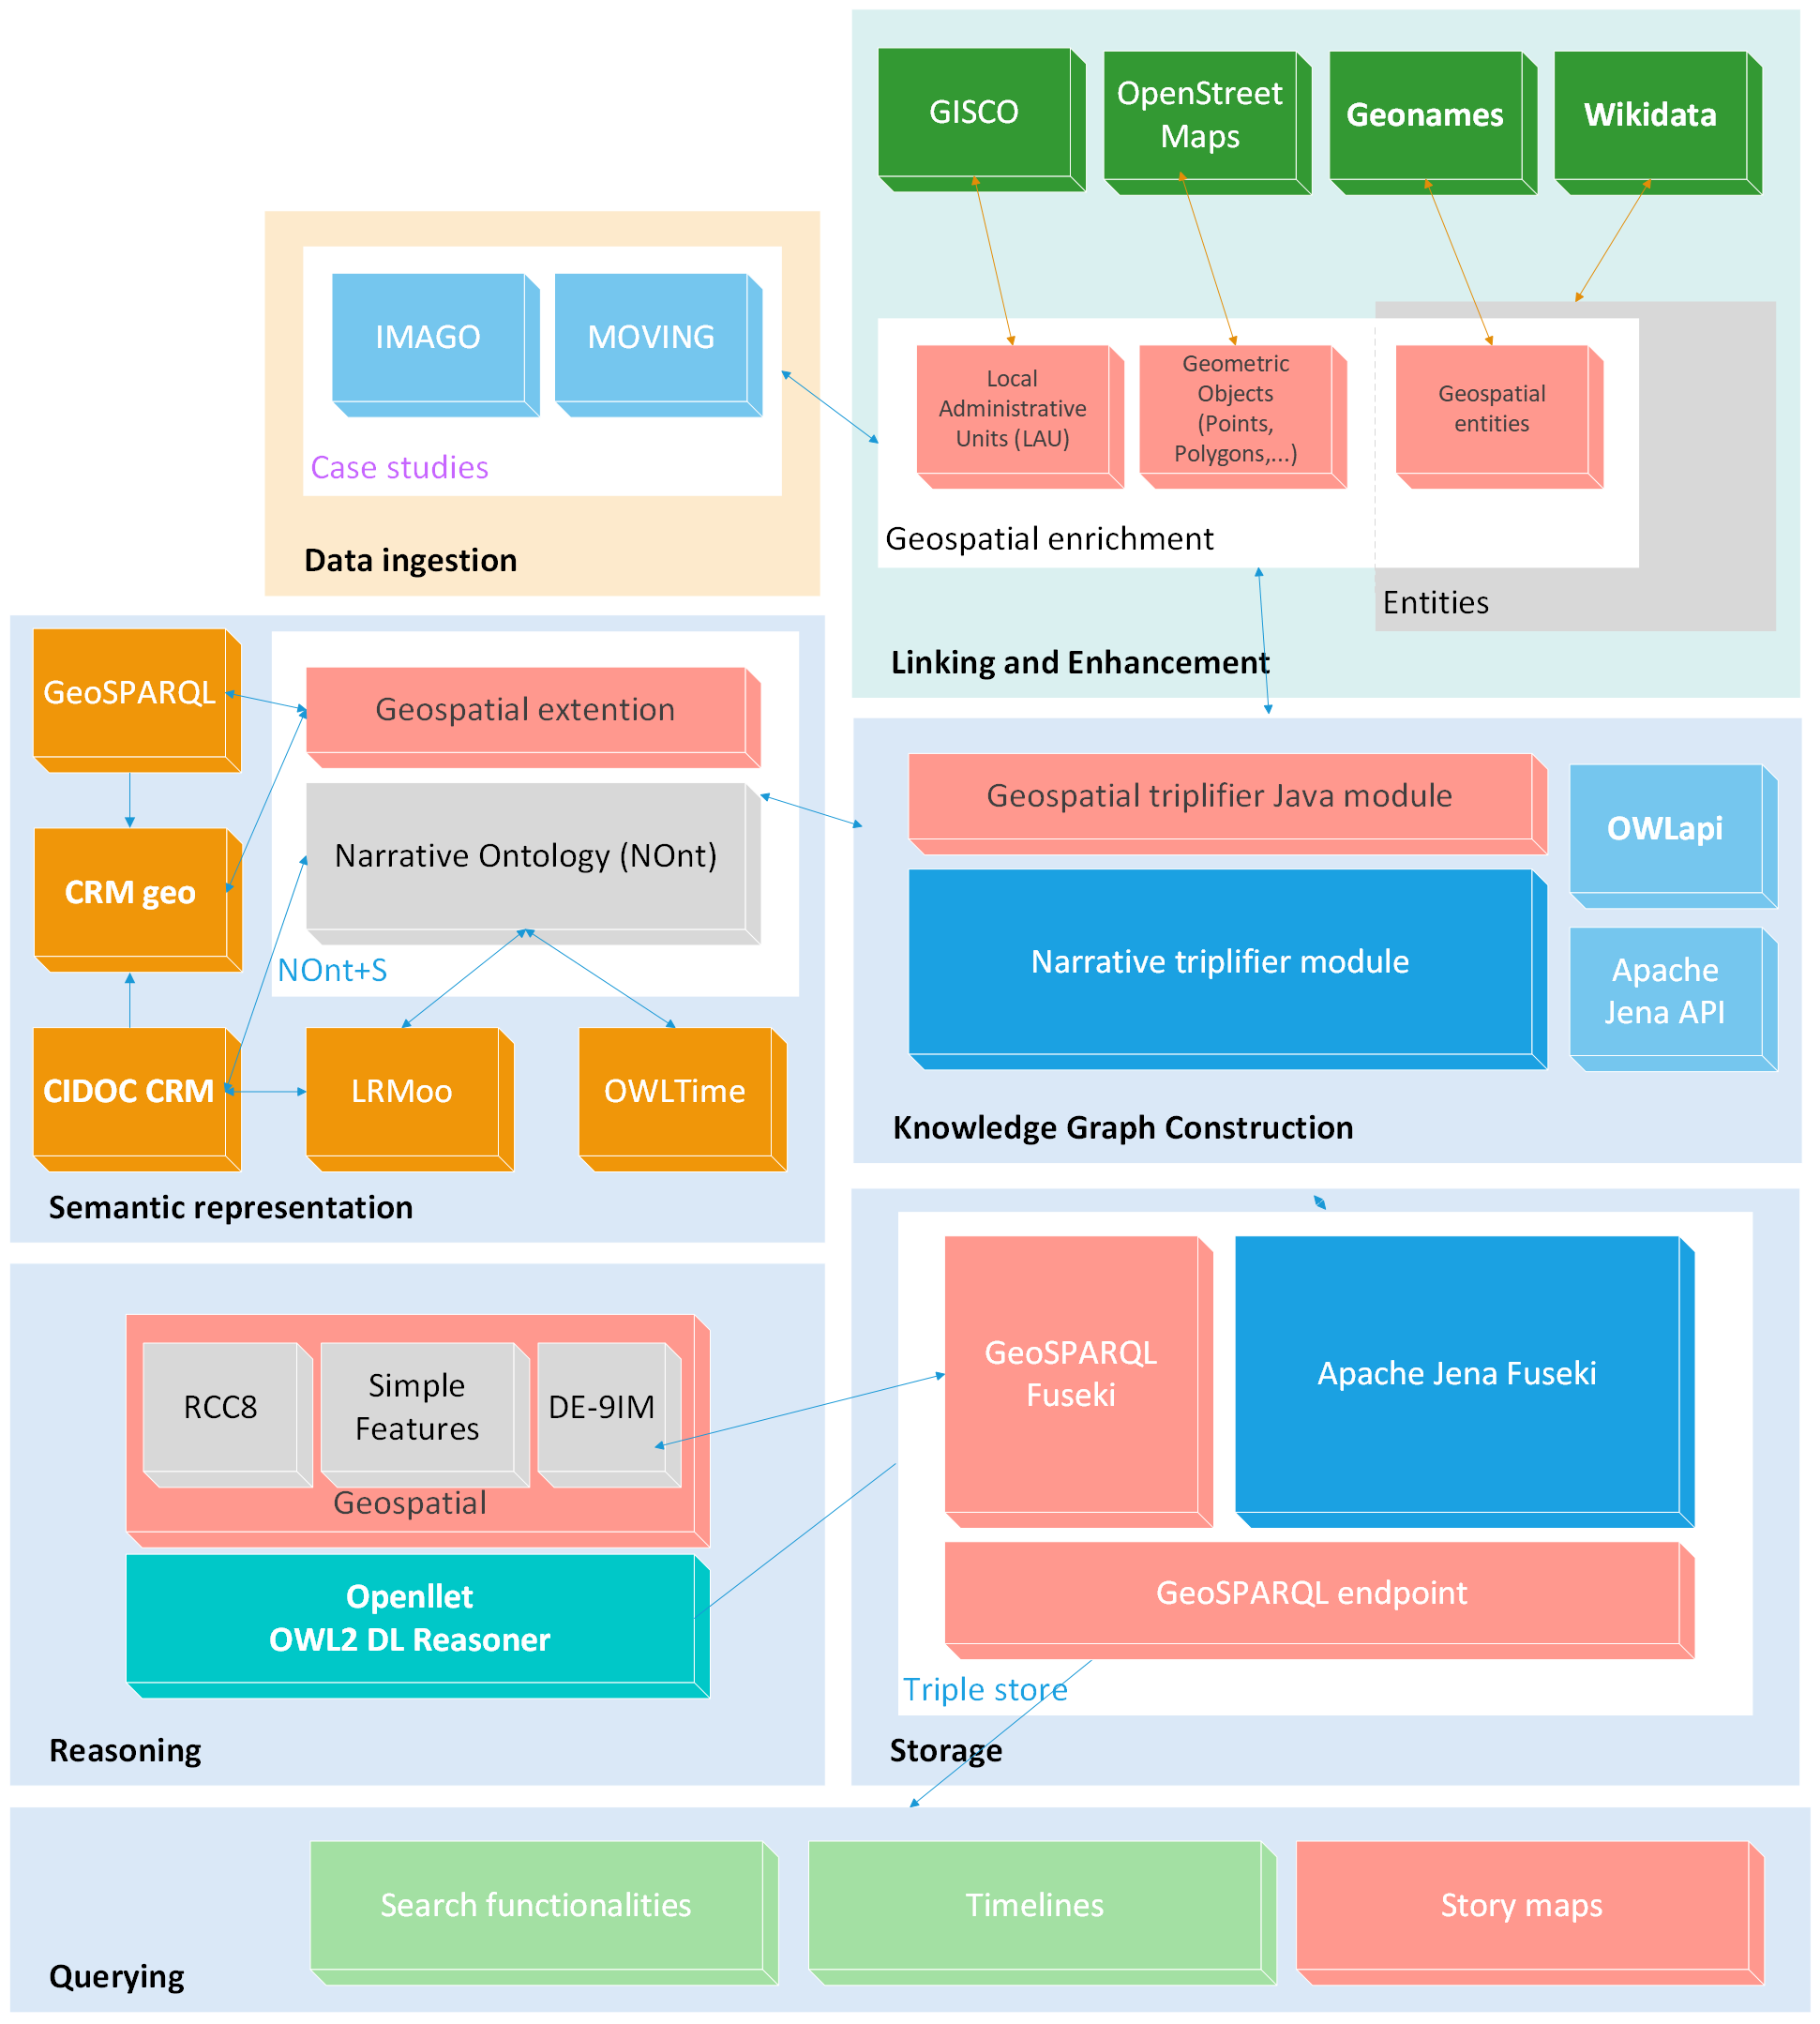
\includegraphics[scale=0.4]{img/SemanticFramework.png}}
    \caption{The image illustrates the semantic web framework of NOnt+S, highlighting its key components: data linking, semantic representation, knowledge graph construction, reasoning, triplestore storage, and advanced querying of geospatial data.}
    \label{fig:SemanticFramework}
\end{figure}

Each of these features is realized through modular components that interact to deliver a scalable and flexible system. The framework consists of six core modules that work in tandem to enable the effective use of geospatial data. These modules are designed to handle distinct tasks, from linking and enriching data to reasoning and querying it. Below, each module is described in detail.

\section{Linking and Enhancement}\label{VI-sec:linking}

The \textit{Linking and Enhancement} module is pivotal in constructing a unified and enriched knowledge graph by integrating data from diverse sources and augmenting it with additional semantic layers. This module ensures that the knowledge graph is both comprehensive and coherent, facilitating seamless integration of heterogeneous datasets into a single, enriched framework. The key tasks performed by this module include entity linking and data enrichment.

\subsection{Entity Linking}\label{VI-subsec:entitylinking}

Entity Linking (EL) is the process of connecting mentions of entities within datasets to their corresponding entities in a knowledge base. This task is essential for aligning semantically similar entities across different datasets, thereby enabling data integration and interoperability.

\subsubsection{Process of Entity Linking}

The entity linking process generally involves three main steps:

\begin{enumerate}
    \item \textbf{Entity Recognition}: Identifying and extracting entity mentions from the dataset. This involves natural language processing techniques to detect names, locations, organizations, and other entity types within unstructured or semi-structured data.
    \item \textbf{Candidate Generation}: For each extracted entity mention, generating a list of potential matching entities from the knowledge base. This step may use string matching, ontological mappings, or semantic similarity measures.
    \item \textbf{Entity Disambiguation}: Selecting the most appropriate entity from the candidate list by considering the context in which the entity mention appears. Techniques such as context vectors, machine learning classifiers, or probabilistic models are employed to determine the best match.
\end{enumerate}

\subsubsection{Linking to Wikidata}

An example of entity linking is connecting dataset entities to \textit{Wikidata} \cite{Wikidata}, an always up-to-date, community-driven, and multilingual knowledge base. Linking to Wikidata enriches the original data by incorporating a wealth of additional information, such as:

\begin{itemize}
    \item \textbf{Semantic Relationships}: Relationships between entities, enabling the inference of new knowledge through connected data.
    \item \textbf{Multilingual Labels}: Support for multiple languages, enhancing accessibility and usability across different linguistic communities.
    \item \textbf{Up-to-Date Information}: Continuous updates by a global community ensure that the data remains current.
\end{itemize}

By linking entities to a comprehensive knowledge base like Wikidata, the module enhances the semantic depth of the knowledge graph and promotes data interoperability.

\subsection{Enrichment}\label{VI-subsec:enrichment}

Enrichment involves augmenting the existing data with additional information to add value and context. In the context of this research, enrichment primarily focuses on adding geospatial information to entities, thereby introducing spatial dimensions to the datasets.


The enrichment process adds qualitative and quantitative spatial data to entities, which includes:

\begin{itemize}
    \item \textbf{Geographic Coordinates}: Adding latitude and longitude to pinpoint exact locations on the Earth's surface.
    \item \textbf{Polygons and Boundaries}: Defining the shape and extent of geographic entities, such as administrative regions, using polygon data.
    \item \textbf{Spatial Relationships}: Describing how entities are spatially related to one another, such as adjacency or containment relationships.
\end{itemize}

Enriching data with geospatial information brings numerous advantages that can significantly enhance the analysis and usability of datasets. One of the key benefits is the improvement in query capabilities. By incorporating spatial data, users can execute complex spatial queries, such as identifying entities within a specific radius or examining the spatial relationships between different entities. These queries allow for more dynamic and context-aware data analysis, which can be essential in applications like urban planning, environmental monitoring, or location-based services.

Another major advantage of geospatial data integration is its power in visualization and mapping. The ability to create detailed maps and spatial visualizations helps reveal patterns and insights that would otherwise remain hidden in non-spatial data. For example, geographic heat maps can highlight areas of high activity or risk, providing decision-makers with visual tools that translate complex data into actionable intelligence. Whether for business logistics, public health, or infrastructure development, geospatial visualizations make the interpretation of data more intuitive and impactful.

Additionally, geospatial enrichment allows for seamless integration with established geospatial standards, promoting compatibility with a wide array of data services. This is critical when working across various platforms or integrating datasets from multiple sources. Standards such as those from the Open Geospatial Consortium (OGC) ensure that enriched datasets can be shared and utilized in a broader context, fostering collaboration and enabling more extensive data interoperability across industries and governmental agencies.

Despite these advantages, the process of linking and enhancing data with geospatial information presents several challenges, each of which requires thoughtful solutions. One significant challenge is the ambiguity that arises when entities from different datasets need to be linked, especially when there are multiple possible matches in a knowledge base. To address this, context-aware disambiguation techniques are employed. Contextual similarity analysis, for instance, involves evaluating surrounding data or text to gather clues that help identify the correct entity. In addition, machine learning models can be trained on labeled datasets to predict the most probable entity matches. These models become increasingly sophisticated as they are exposed to more data, improving the accuracy of entity linking over time.

Another challenge stems from the fact that datasets sourced from various platforms often differ in format, schema, and overall quality. Standardization and normalization are critical processes to overcome these disparities. Aligning schemas involves using ontologies and data models to harmonize the data structures, ensuring that disparate datasets can be effectively merged or compared. Meanwhile, data cleaning techniques are employed to eliminate inconsistencies and errors, thereby enhancing the overall quality and reliability of the data. These processes ensure that the enriched dataset is not only comprehensive but also consistent and accurate, which is essential for any meaningful analysis.

Finally, processing large volumes of geospatial data requires substantial computational resources and efficient algorithms. To manage this, distributed computing frameworks such as Apache Hadoop or Spark can be utilized, enabling parallel processing across multiple nodes. This approach significantly reduces the time required for data processing, especially when handling big data. Additionally, the use of optimized algorithms with favorable time and space complexity ensures that operations are performed efficiently, minimizing computational overhead while maximizing performance. These solutions help address the scalability issues inherent in working with large datasets, ensuring that geospatial data enrichment can be applied even in resource-intensive environments.

By addressing these challenges with advanced techniques and solutions, the process of enriching data with geospatial information becomes more feasible, allowing organizations to unlock the full potential of their data for more informed decision-making.

\section{Semantic Representation}\label{VI-sec:semantic-representation}

At the core of the framework lies the \textit{Semantic Representation} module, which employs the NOnt+S ontology to structure and organize data. This module offers the formal representation of knowledge within narratives, ensuring that narrative concepts are accurately represented in the corresponding knowledge graph. A key feature of this module is its ability to integrate geospatial representations into the knowledge structure. As detailed in \ref{chap:nont+s}, the NOnt+S ontology provides an extensive and well-defined vocabulary for modeling geospatial entities, along with their associated attributes and relationships, thereby facilitating a comprehensive representation of both narrative and spatial elements within the semantic framework.

\section{Knowledge Graph Construction}\label{VI-sec:KG}

After the data has been semantically enriched and properly represented, the next crucial step involves the construction of the knowledge graph. This process is managed by the \textit{Knowledge Graph Construction} module, which is responsible for organizing the enriched data into a coherent graph-based structure. The purpose of this step is to translate the complex, interconnected information into a format that accurately represents geospatial entities and their relationships. The result is a formal structure using \acrshort{OWLLabel}2 DL (Web Ontology Language, Description Logic) \cite{OWLWebOntologyc}.

At the core of this process, the module utilizes two essential tools: the Apache Jena API\cite{ApacheJenaFramework} and the OWLapi\cite{OwlcsOwlapi2024}. Apache Jena is a widely-used framework that facilitates the creation and manipulation of RDF (Resource Description Framework) graphs, while OWLapi is specifically designed to handle \acrshort{OWLLabel} ontologies. Together, these technologies form the backbone of the knowledge graph construction process, enabling the seamless conversion of the enriched data into a robust, ontology-based structure.

One of the module's key components, the \textit{triplifier} software, plays a significant role in this transformation. The triplifier software converts the enriched data into RDF triples, the building blocks of the knowledge graph. These triples represent subject-predicate-object relationships, providing a flexible and scalable means of capturing complex data. 

Particularly noteworthy is the role of the \textit{geospatial triplifier} software within the module. This specialized component is designed to manage geospatial data by facilitating the conversion between various spatial data formats, such as \acrfull{WKTLabel}\cite{WellknownTextRepresentationa} and \acrfull{GMLLabel}\cite{GeographyMarkupLanguagea}. WKT and GML are common standards for representing spatial information, and their compatibility with the knowledge graph format is essential for ensuring that the spatial relationships between entities are maintained and accurately reflected in the graph. Through this process, the geospatial triplifier software enables the seamless integration of location-based data into the overall knowledge graph, allowing for sophisticated queries and reasoning over geospatial entities and their interconnections.

\section{Reasoning}\label{VI-sec:reasoning}

The \textit{Reasoning} module is a critical component of the framework, enabling semantic reasoning, which is the process of deriving new insights from existing data. This ability to infer new facts is based on predefined inference rules or ontologies, allowing for the enrichment of the knowledge graph. By introducing new knowledge and adding context, the module enhances the dataset’s depth and usability. The Reasoning module goes beyond mere data retrieval; it transforms a static repository into an intelligent system capable of generating additional information and insights from the given data. Furthermore, it integrates geospatial reasoning, extending its utility to spatial data and relationships.


The Reasoning module provides two key capabilities that empower the framework to extend the meaning and utility of the data: Geospatial Reasoning and Semantic Reasoning.

\subsection{Geospatial Reasoning}\label{VI-subsec:geospatialReasoning}

Geospatial reasoning is a critical component of the framework, as it enables the system to derive meaningful inferences about spatial relationships and configurations from annotated geographical data. This form of reasoning extends beyond simple location retrieval; it encompasses the ability to interpret spatial properties and to draw both quantitative and qualitative conclusions about the relative positions, distances, and spatial hierarchies among entities. By harnessing geospatial reasoning, the system can address complex queries, such as identifying proximity between historical sites, detecting overlaps in territorial boundaries, or establishing containment relationships between regions.

The process of geospatial reasoning integrates seamlessly with the GeoSPARQL standard, which provides a robust model for representing and querying geospatial information within OWL graphs. GeoSPARQL’s capabilities facilitate the interpretation of both explicit geospatial data, such as coordinates or polygon geometries, and implicit spatial relationships that can be inferred through reasoning mechanisms. For example, when analyzing medieval or Renaissance geographical texts, the system can infer that a particular site lies within a specified historical region based on its coordinates or can recognize spatial patterns among multiple places that share a common historical significance.

\subsection{Semantic Reasoning}\label{VI-subsec:semanticReasoning}

Semantic reasoning in the framework is powered by the well-established semantic web reasoning engines  Pellet\cite{sirinPelletPracticalOWLDL2007} implemented thought the open source implementation Openllet\cite{galigatorGaligatorOpenllet2024}. This engine enable the automated inference of new knowledge from existing data by applying formal rules defined within ontologies. Semantic reasoning plays a pivotal role in ensuring that the knowledge graph remains logically consistent and that complex relationships between entities can be accurately inferred.

By employing these reasoners, the system can validate ontology constraints, perform class subsumption checks, and infer implicit relationships, thereby enhancing the expressiveness and utility of the knowledge graph. For instance, if a geographical work is associated with a particular cultural heritage site through a set of ontological properties, semantic reasoning can automatically classify and link related entities, revealing deeper connections that may not be immediately apparent.

Moreover, these reasoning engines support rule-based and ontology-based inferences, which are instrumental in managing the complexity of geospatial narrative data. This level of semantic reasoning ensures that the knowledge graph serves as a rich and cohesive resource, empowering researchers to perform sophisticated queries and gain insights that are grounded in a rigorous semantic framework.

\section{Storage}\label{VI-sec:storage}

In the domain of knowledge representation and the Semantic Web, triplestores play a fundamental role in storing and querying structured data. 
In modern knowledge representation systems, managing enriched and semantically structured data requires an efficient, scalable, and reliable storage solution. This chapter describes the storage module of the framework, which leverages a triplestore to handle \acrshort{OWLLabel} triples that form the backbone of the knowledge graph. A triplestore is a database specifically designed for storing and managing \acrshort{RDFLabel}/\acrshort{OWLLabel} triples, making it particularly well-suited for knowledge graphs that require efficient querying, scalability, and the ability to manage complex, interconnected datasets.

A triplestore serves as the fundamental storage component of the framework, managing \acrshort{OWLLabel} triples, where each triple consists of a subject, predicate, and object. This structure allows for the flexible representation of relationships and properties in a semantic format, enabling sophisticated knowledge representation. In the context of this framework, the triplestore ensures that the knowledge graph remains accessible and performant, even as it scales to accommodate large and complex datasets, such as geospatial data. The Storage module is designed with two critical capabilities: efficient data retrieval and scalability. These features ensure the triplestore can handle the demands of storing and querying semantically rich, interconnected data. Triplestores are optimized for querying large volumes of \acrshort{RDFLabel} triples, making them ideal for use cases that involve extensive, highly interconnected data, such as geospatial knowledge graphs. The framework utilizes \acrshort{SPARQLLabel}\cite{ericprudhommeauxSPARQLQueryLanguage2008}, a powerful query language specifically designed for \acrshort{RDFLabel} data, to retrieve information from the triplestore. The inherent efficiency of triplestores in executing complex queries enables fast data retrieval, even in scenarios where relationships span numerous triples. As the amount of data ingested into the system grows, the triplestore must scale accordingly. The framework's triplestore is designed to handle increasing volumes of \acrshort{OWLLabel} triples without compromising performance. This scalability is particularly important for knowledge graphs in domains such as geospatial analysis, where large datasets are common, and the ability to maintain performance with growing data volumes is critical.

\subsection{Implementation: Fuseki and GeoSPARQL Support}\label{VI-subsec:fuseki}

Fuseki is the triplestore component of the Apache Jena framework, an open-source and widely adopted Java-based platform for building Semantic Web applications \cite{ApacheJenaFramework}. As part of Apache Jena, Fuseki provides robust capabilities for storing, managing, and querying \acrshort{RDFLabel} datasets, specifically through its support for the \acrshort{SPARQLLabel} query language \cite{ApacheJenaFuseki}. It is particularly well-suited for Semantic Web use cases, where \acrshort{RDFLabel} serves as the foundational data model and \acrshort{SPARQLLabel} as the query language. Fuseki offers key features that facilitate efficient data management and retrieval for Semantic Web projects:

\begin{itemize}
    \item \textbf{\acrshort{SPARQLLabel} 1.1 Compliance}: Fuseki fully implements the \acrshort{SPARQLLabel} 1.1 standard, enabling comprehensive support for various query types such as SELECT, CONSTRUCT, ASK, and UPDATE, thereby allowing sophisticated interaction with \acrshort{RDFLabel} data.
    \item \textbf{HTTP Protocol Integration}: It provides an HTTP interface, enabling \acrshort{SPARQLLabel} queries to be executed and results retrieved over the web, which is particularly useful for web-based Semantic Web applications.
    \item \textbf{Flexible Data Storage}: Fuseki supports multiple storage options, including in-memory and persistent stores, giving developers the flexibility to choose the appropriate storage backend based on application requirements.
    \item \textbf{Modularity and Extensibility}: Highly modular by design, Fuseki allows for easy extension with custom functionalities, enabling developers to incorporate additional data processing standards such as GeoSPARQL \cite{GeoSPARQLFuseki}.
\end{itemize}

As outlined in chapter \ref{chap:theoretical_framework}, GeoSPARQL is an OGC standard designed to extend SPARQL with the capability to represent and query geospatial data. It introduces geospatial vocabularies, filters, and topological functions, allowing \acrshort{RDFLabel} datasets to manage spatial information \cite{matthewperryOGCGeoSPARQLGeographic2012}. The GeoSPARQL Fuseki extension integrates this standard into the Fuseki triplestore, enabling the execution of geospatial queries through the standard Fuseki HTTP server or as an embedded component \cite{GeoSPARQLFuseki}. This extension ensures full compliance with the GeoSPARQL standard, allowing users to perform spatial queries on \acrshort{OWLLabel} datasets using \acrshort{SPARQLLabel} enriched with geospatial functions. 

GeoSPARQL Fuseki’s HTTP interface supports all relevant GeoSPARQL predicates and functions, simplifying its integration with existing web services and applications. Furthermore, its modularity allows it to be embedded within Fuseki’s core, enabling developers to add geospatial querying capabilities to their \acrshort{RDFLabel} datasets without the need to run a separate service. This adaptability underscores Fuseki's strength in supporting diverse and evolving needs within Semantic Web and geospatial data applications.

\subsection{GeoSPARQL Compliance Testing}\label{VI-subsec:compliance-geosparql}

To ensure that the triplestore implementation adheres to the required standards, we conducted a GeoSPARQL compliance test. Compliance with GeoSPARQL guarantees that a triplestore can effectively store, manage, and query geospatial data in line with the requirements established by GeoSPARQL \acrshort{OGCLabel} standard\cite{GeoSPARQLGeographicQuerya}. Verifying compliance involves benchmarking the system against a set of criteria defined by the GeoSPARQL specification. Jovanovik et al. \cite{jovanovikGeoSPARQLComplianceBenchmark2021a} proposed a benchmark designed to evaluate the compliance of various triplestores with the GeoSPARQL standard. When our implementation was tested using this framework, the results showed a compliance level comparable to those reported in prior studies, confirming that our triplestore meets many of the core GeoSPARQL requirements. However, the results also revealed that certain aspects of the GeoSPARQL specification are not fully supported by the triplestore.

\begin{table}[ht]
\centering \caption{Triplestore Feature Comparison}
\label{tab:triplestore-comparison}
\vskip 0.2cm
\scalebox{0.90}{
\begin{tabular}{|l|c|c|c|c|c|c|}
\hline
\textbf{Triplestore}      & \textbf{CORE} & \textbf{TOP} & \textbf{GEOEXT}               & \textbf{GTOP}                 & \textbf{RDFSE} & \textbf{QRW}  \\ \hline
GeoSPARQL Fuseki          & Full          & Full         & Full/E                        & Full                          & Full           & Full/E        \\ \hline
GraphDB          & Full          & Full         & Partial [WKT]                 & Partial [WKT]                 & Full           & None          \\ \hline
Strabon          & Full          & Full         & Partial [WKT]                 & Partial [WKT]                 & Full           & None          \\ \hline
Virtuoso         & Full          & Full         & Partial [WKT]                 & Partial [WKT]                 & Full           & None          \\ \hline
TriplyDB                  & Full          & Full         & Partial [WKT]                 & Partial [WKT]                 & Full           & None          \\ \hline
RDF4J   c          & Full          & Full         & Partial [WKT CRS84]           & Partial [WKT CRS84]           & Full           & None          \\ \hline

\end{tabular}
}
\end{table}

In addition, we applied\footnote{The code for replicating the evaluation is available on GitHub at \url{https://github.com/prate91/Geosparql2benchmark}} the benchmark to Strabon, a system not previously evaluated by Jovanovik et al., which supports both GeoSPARQL and stSPARQL\cite{koubarakisModelingQueryingMetadata2010a}. To better understand the variations in compliance across different systems, we analyzed the benchmark results with respect to the six extensions defined in the GeoSPARQL specification. Table \ref{tab:triplestore-comparison} summarizes the results for major triplestores that support at least partial implementations of the Geometry Extension (GEOEXT) and Geometry Topology (GTOP). The core components and extensions of GeoSPARQL are briefly described as follows. The Core component (CORE) defines the foundational spatial vocabulary elements, while the Topology vocabulary extension (TOP) specifies the vocabulary for topological relations. The Geometry Extension (GEOEXT) provides vocabulary for geometry and non-topological query functions, and the Geometry Topology extension (GTOP) defines topological query functions for geometry objects. The \acrshort{RDFSLabel} Entailment Extension (RDFSE) introduces mechanisms to match inferred RDF triples based on \acrshort{RDFLabel} and \acrshort{RDFSLabel} semantics, enabling reasoning through \acrshort{RDFSLabel}. Finally, the Query Rewrite extension (QRW) specifies rules for transforming queries to compute spatial relations between objects based on their geometries.

Among the triplestores tested, GeoSPARQL Fuseki demonstrated the highest level of compliance, consistently outperforming other systems in overall GeoSPARQL support. It was the only triplestore that fully supported both \acrshort{GMLLabel} and \acrshort{WKTLabel} formats, as well as the only one that implemented all GeoSPARQL extensions. However, despite these strengths, GeoSPARQL Fuseki exhibited certain limitations during the benchmark tests. Specifically, it returned incorrect results for certain functions within the Query Rewrite (QRW) and Geometry (GEOEXT) extensions. These issues indicate the need for further optimization to fully support advanced GeoSPARQL functionalities, particularly in the areas of geometry handling and query rewriting.

A significant problem identified by the benchmark was GeoSPARQL Fuseki’s inability to handle empty WKT and GML literals—an issue observed across all triplestores tested. Proper handling of empty literals is essential for ensuring robust GeoSPARQL support, as it directly impacts the accuracy and reliability of query results, particularly when working with complex geospatial datasets. Addressing this limitation is critical for enhancing the overall reliability and functionality of GeoSPARQL implementations.

\subsection{Performance Benchmarking with GeoSPARQL Fuseki}\label{VI-subsec:performance-geosparql}

In addition to compliance testing, the performance of the framework with GeoSPARQL Fuseki was evaluated using the benchmarking tool \textit{Geographica 2}\cite{ioannidisEvaluatingGeospatialRDF2021}. This benchmark is designed to assess the performance of triplestores in processing geospatial queries, with a particular focus on query execution time and scalability when handling large geospatial datasets. While many triplestores such as Strabon, uSeek, Parliament, System X, GraphDB, and RDF4J have been tested with this benchmark, GeoSPARQL Fuseki has not yet been evaluated within this framework.

We implemented the test of GeoSPARQL Fuseki in two distinct configurations to assess its performance in two differents use cases. The first one is in localhost on windows, trying to assess the performance without the connection to a server (configuration 1). The second configuration is on a server platform served through tomcat9, accessible through an endpoint. The two configurations are shown in Table \ref{tab:triplestore-performance-configuration}:

\begin{table}[ht]
\centering \caption{System Configurations for GeoSPARQL Fuseki Performance Testing}
\label{tab:triplestore-performance-configuration}
\vskip 0.2cm
\scalebox{0.90}{
\begin{tabular}{|l|c|c|}
\hline
\textbf{Component}          & \textbf{Configuration 1}                                    & \textbf{Configuration 2}                                    \\ \hline
\textbf{Platform}           & Windows 10.0.22635 (AMD64)                                  & Linux (Ubuntu 5.15.0-117-generic)                           \\ \hline
\textbf{Processor Model}    & 11th Gen Intel\textsuperscript{\tiny\textregistered} Core\textsuperscript{\texttrademark} i7-1165G7                        & Intel\textsuperscript{\tiny\textregistered} Xeon\textsuperscript{\tiny\textregistered} CPU E5-4610 v2                             \\ \hline
\textbf{Base Frequency}     & 2.80 GHz                                                    & 2.30 GHz                                                    \\ \hline
\textbf{Architecture}       & x86-64 (AMD64)                                              & x86-64                                                      \\ \hline
\textbf{Microarchitecture}  & Tiger Lake                                                  & Ivy Bridge                                                  \\ \hline
\textbf{Physical Cores}     & 4                                                           & 2                                                           \\ \hline
\textbf{Total Cores}        & 8                                                           & 2                                                           \\ \hline
\textbf{RAM}                & 16 GB                                                       & 16 GB                                                       \\ \hline
\end{tabular}
}
\end{table}

Before presenting the results of this benchmark on the two configurations, we briefly present the relevant concepts of the Geographica2 benchmark. For a comprehensive explanation of the benchmark and its full evaluation, please refer to Ioannidis et al. \cite{ioannidisEvaluatingGeospatialRDF2021}. The benchmark tests real-world, synthetic, and scalability workloads, each focusing on different aspects of \acrshort{RDFLabel} store performance.

To benchmark \acrshort{RDFLabel} stores accurately, Geographica 2 uses a variety of datasets, including real-world data from \acrfull{LODLabel} and specialized datasets with complex geometries. These datasets help simulate real-world geospatial tasks and provide the basis for the workloads. The real datasets employed by the benchmark are divided into three groups: \acrshort{LODLabel} datasets, datasets with complex geometries and specialized datasets. In the first group, there is (i) DBpedia\cite{DBpedia2024}, a crowd-sourced knowledge base derived from Wikipedia that contains geospatial information in the form of point geometries (e.g., cities, buildings); (ii) GeoNames\cite{GeoNames}, a global geographical database with over 11 million unique features that provide point geometries representing cities, lakes, and landmarks, with coordinates in the WGS84 \acrshort{CRSLabel}, and \acrfull{LGDLabel}\cite{LinkedGeoData}, based on \acrfull{OSMLabel}\cite{OpenStreetMap} that includes features such as motorways, rivers, and geographic entities. Then, in the second group, there is (i) \acrfull{GAGLabel}\cite{GreekAdministrativeGeography}, a dataset containing polygon geometries representing municipalities in Greece, crucial for spatial join operations; (ii) \acrfull{CLCLabel}\cite{CORINELandCover}, a dataset from the European Environmental Agency with complex polygon geometries representing land cover across Europe; and (iii) Wildfire Hotspot Dataset\cite{sifakisWildfireDetectionTracking2011}, developed by the National Observatory of Athens that consists of polygons representing wildfire areas, derived from \acrfull{EOLabel} data. Finally, the third group is compose only by Census Dataset, sourced from the U.S. Census Bureau, includes the street network data of New York City. Streets are represented as linestrings, with detailed address ranges, enabling geocoding operations.

The real datasets are employed in the real-world workload that simulates common geospatial tasks in order to evaluate how efficiently stores handle geospatial queries involving \acrshort{LODLabel}, spatial joins, and polygon and point operations. The real-world workload is divided into micro benchmark and macro benchmark. The micro benchmark tests the efficiency of basic spatial functions in geospatial triplestores using simple GeoSPARQL queries. The comprehensive set of queries designed for evaluating the performance of geospatial systems, as discussed in \cite{ioannidisEvaluatingGeospatialRDF2021}, comprises 29 distinct queries. These queries are systematically categorized into four primary groups. However, for our performance assessment using Fuseki GeoSPARQL, we limited the evaluation to three of these groups, excluding the fourth, which focuses on Aggregate Functions\footnote{The queries for this group are available at \url{https://geographica2.di.uoa.gr/queries/micro_aggregations.lst}}. This group (Q28 and Q29) exclusively utilizes the stSPARQL operator and is thus not pertinent to our comparative analysis. Specifically, the first group, denoted as \acrfull{NTCFLabel}\footnote{The queries for this group can be accessed at \url{https://geographica2.di.uoa.gr/queries/micro_nontopological.lst}}, encompasses queries Q1 to Q6 and addresses non-topological conditions. The second group, labeled as \acrfull{SSLabel}\footnote{The queries for this group are available at \url{https://geographica2.di.uoa.gr/queries/micro_selections.lst}}, spans from Q7 to Q17, focusing on selection-based geospatial queries. Finally, the third group, \acrfull{SJLabel}\footnote{The queries for this group can be consulted at \url{https://geographica2.di.uoa.gr/queries/micro_joins.lst}}, includes queries Q18 to Q27, which are structured around join operations within geospatial datasets.
The macro benchmark evaluates geospatial triplestores in complex real-world applications, such as geocoding, reverse geocoding, map search and browsing, and earth observation scenarios.

There is also a synthetic workload that tests system performance using artificially generated datasets and queries. This workload includes two key metrics: data scalability, which tests the system's response as the dataset size increases, and query selectivity, which evaluates performance based on varying levels of query selectivity. In this workload, the queries are built based on the query template shown in \ref{lst:template-synthetic} to produce SPARQL queries corresponding to spatial selections that ask for land ownerships which intersect a given rectangle and points of interest that are within a given rectangle. The given rectangle is generated in such a way that the spatial predicate of the query holds for 0.01\%, 10\%, 25\%, 50\%, or 75\% of all the features of the respective dataset. In addition, the query template was instantiated using the extreme values 1 and 512 for the parameter THEMA, selecting either all or approximately 0.02\% of the total features of a dataset.

\begin{lstlisting}[caption=Template to build queries for synthetic workload from \cite{ioannidisEvaluatingGeospatialRDF2021}, label={lst:template-synthetic}]
 SELECT ?s
    WHERE{ 
    ?s ns:hasGeometry/ns:asWKT ?g.
    ?s c:hasTag/ns:hasKey "THEMA".
    FILTER(FUNCTION(?g, "GEOM"))}
\end{lstlisting}

Eventually, there is the Scalability Workload that assesses how the system handles increasingly large datasets. The metrics include storage efficiency, evaluating how efficiently large datasets are stored, bulk loading time, measuring the time to load large datasets and query response Time, and analyzing how query performance scales as data volume increases.

\subsection{Geographica2 Results for GeoSPARQL Fuseki}\label{VI-subsec:geographica2-results}

The evaluation results\footnote{The code for replicating the evaluation is available on GitHub at \url{https://github.com/prate91/Geosparql2benchmark} and \url{https://github.com/prate91/geographica2}} indicate that GeoSPARQL Fuseki demonstrates strong performance across various types of geospatial queries, affirming its capability to handle increased geospatial data efficiently. This efficiency positions it as a suitable choice for real-time analysis within the Semantic Web framework. A detailed examination of the data reveals several patterns in performance based on query type and specific query configurations.

In \acrshort{NTCFLabel}, GeoSPARQL Fuseki outperformed other triplestores in many cases, particularly from Q2 to Q6. This advantage highlights its capability to manage non-topological query processing with notable efficiency, a critical aspect for systems requiring rapid responses to spatial data without complex relational dependencies. The configuration variations of Fuseki also show consistent improvement, with configuration 2 slightly surpassing configuration 1 in response times across these queries.


 \begin{table}[h!tb]
   \centering \caption{Performance (seconds) of Triple Stores.
The symbols represent performance percentiles: \ding{115} indicates values between the 33rd and 67th percentiles, \ding{108} denotes values below the 33rd percentile, and \ding{110} represents values above the 67th percentile. Performance data for triple stores other than Fuseki is sourced from the Geographica2 benchmark.}
\label{table:cold_caches}
   \vskip 0.2cm
   %%
   \scalebox{0.90}{
	    %% The {|c|c|c|c|c|} define the number of columns.
	    %% c means centered
	    %% | defines a vertical line between two columns 
	    \begin{tabular}{|c|c|r|r|r|r|r|r|}
        \hline
	     Type & Query & Strabon & GraphDB & RDF4J & RDF4J (L) & Fuseki (c1) & Fuseki (c2) \\ \hline
NTCF & Q1 & \ding{115} 42.33 & \ding{108} 29.68 & \ding{115} 37.24 & \ding{115} 37.34 & \ding{110} 50.78 & \ding{110} 52.44 \\
              & Q2 & \ding{110} 22.48 & \ding{108} 14.55 & \ding{115} 18.41 & \ding{115} 18.75 & \ding{108} 12.24 & \ding{110} 25.31 \\
              & Q3 & \ding{110} 29.48 & \ding{108} 19.42 & \ding{115} 24.57 & \ding{115} 24.56 & \ding{108} 18.26 & \ding{110} 31.04 \\
              & Q4 & \ding{110} 7.65 & \ding{108} 3.20 & \ding{108} 3.32 & \ding{108} 3.48 & \ding{108} 2.72 & \ding{108} 4.26 \\
              & Q5 & \ding{110} 14.68 & \ding{115} 7.45 & \ding{108} 4.52 & \ding{108} 4.64 & \ding{108} 3.00 & \ding{108} 4.46 \\
              & Q6 & \ding{110} 23.82 & \ding{115} 13.53 & \ding{110} - & \ding{110} - & \ding{108} 0.25 & \ding{108} 0.17 \\ \hline
SS & Q7 & \ding{108} 0.36 & \ding{110} 5.33 & \ding{115} 3.64 & \ding{110} 3.97 & \ding{110} 5.71 & \ding{108} 0.77 \\
              & Q8 & \ding{108} 0.42 & \ding{110} 2.04 & \ding{110} 1.76 & \ding{110} 1.78 & \ding{110} 2.36 & \ding{115} 1.67 \\
              & Q9 & \ding{108} 0.83 & \ding{110} 28.28 & \ding{110} 40.46 & \ding{110} 40.60 & \ding{110} 38.42 & \ding{108} 3.75 \\
              & Q10 & \ding{108} 0.73 & \ding{110} 22.24 & \ding{110} 25.40 & \ding{110} 25.24 & \ding{110} 19.74 & \ding{110} 23.61 \\
              & Q11 & \ding{108} 2.66 & \ding{110} 114.29 & \ding{110} 164.48 & \ding{110} 164.84 & \ding{110} 154.94 & \ding{108} 35.76 \\
              & Q12 & \ding{115} 0.79 & \ding{110} 1.02 & \ding{108} 0.65 & \ding{108} 0.67 & \ding{115} 0.80 & \ding{108} 0.63 \\
              & Q13 & \ding{108} 0.82 & \ding{110} 49.67 & \ding{110} 72.89 & \ding{110} 72.20 & \ding{110} 70.89 & \ding{108} 6.74 \\
              & Q14 & \ding{108} 0.50 & \ding{108} 4.13 & \ding{108} 1.85 & \ding{108} 1.90 & \ding{110} 63.84 & \ding{108} 7.08 \\
              & Q15 & \ding{108} 0.50 & \ding{110} 0.93 & \ding{108} 0.44 & \ding{108} 0.48 & \ding{115} 0.67 & \ding{108} 0.58 \\
              & Q16 & \ding{108} 2.79 & \ding{115} 50.61 & \ding{110} 72.86 & \ding{110} 72.34 & \ding{110} 82.39 & \ding{108} 7.46 \\
              & Q17 & \ding{108} 3.06 & \ding{115} 28.31 & \ding{110} 40.41 & \ding{110} 40.06 & \ding{110} 45.34 & \ding{108} 4.72 \\ \hline
SJ & Q18 & \ding{108} 4.52 & \ding{108} 942.89 & \ding{110} 2894.56 & \ding{110} 2885.72 & \ding{108} 450.00 & \ding{110} - \\
              & Q19 & \ding{108} 1272.54 & \ding{110} \textgreater 3600 & \ding{110} \textgreater 3600 & \ding{110} \textgreater 3600 & \ding{110} 3010.62 & \ding{110} - \\
              & Q20 & \ding{108} 115.93 & \ding{110} \textgreater 3600 & \ding{110} \textgreater 3600 & \ding{110} \textgreater 3600 & \ding{110} \textgreater 3600 & \ding{108} 147.91 \\
              & Q21 & \ding{108} 113.26 & \ding{110} \textgreater 3600 & \ding{110} \textgreater 3600 & \ding{110} \textgreater 3600 & \ding{110} \textgreater 3600 & \ding{108} 86.64 \\
              & Q22 & \ding{108} 26.33 & \ding{110} \textgreater 3600 & \ding{110} \textgreater 3600 & \ding{110} \textgreater 3600 & \ding{110} \textgreater 3600 & \ding{108} 227.49 \\
              & Q23 & \ding{108} 26.29 & \ding{110} \textgreater 3600 & \ding{110} \textgreater 3600 & \ding{110} \textgreater 3600 & \ding{110} \textgreater 3600 & \ding{108} 118.01 \\
              & Q24 & \ding{108} 26.66 & \ding{110} \textgreater 3600 & \ding{110} \textgreater 3600 & \ding{110} \textgreater 3600 & \ding{110} \textgreater 3600 & \ding{108} 728.56 \\
              & Q25 & \ding{108} 342.87 & \ding{110} \textgreater 3600 & \ding{110} \textgreater 3600 & \ding{110} \textgreater 3600 & \ding{110} \textgreater 3600 & \ding{108} 701.85 \\
              & Q26 & \ding{115} 343.30 & \ding{110} 466.86 & \ding{115} 326.22 & \ding{115} 324.79 & \ding{110} 520.40 & \ding{108} 52.39 \\
              & Q27 & \ding{108} 343.72 & \ding{110} \textgreater 3600 & \ding{110} \textgreater 3600 & \ding{110} \textgreater 3600 & \ding{110} \textgreater 3600 & \ding{110} - \\ \hline
\end{tabular}
	 }
 \end{table}


For \acrshort{SSLabel}, GeoSPARQL Fuseki maintains competitive performance, closely following Strabon, which holds the leading position. Fuseki’s performance in this category indicates that it can handle spatial selection queries, which involve filtering spatial data based on specific criteria, with an efficiency that supports high-throughput applications. The superior response times in comparison to most other triplestores further underscore its reliability for query-intensive applications where response latency needs minimization.

In the case of \acrshort{SJLabel}, where the queries are more computationally demanding due to the need to correlate multiple datasets based on spatial relationships, GeoSPARQL Fuseki also performed commendably, showing a reasonable capacity to manage these complex operations. Although some queries (such as Q18 and Q20) reveal limits in performance under extremely high data loads, GeoSPARQL Fuseki generally demonstrates a balanced trade-off between processing time and data handling capabilities. For certain high-demand join queries, response times show a higher latency, particularly in comparison to simpler queries; however, the results suggest that Fuseki remains feasible for scenarios where occasional high-complexity queries are required within a primarily non-join-intensive workload.

The results summarized in Table~\ref{table:cold_caches} offer a comprehensive view of the comparative performance across a range of queries under different configurations and provide a robust indication of GeoSPARQL Fuseki’s role in scalable and efficient geospatial data processing. These findings collectively validate GeoSPARQL Fuseki as a capable tool within a spatially-enabled Semantic Web environment, especially for applications with mixed workloads of non-topological and spatial selection queries.

\begin{table}[ht]
\centering \caption{Storing times (sec.)}
\label{tab:triplestore-storing-times}
\vskip 0.2cm
\scalebox{0.90}{
\begin{tabular}{|l|c|c|c|c|c|c|}
\hline
Datasets & Strabon  &  GraphDB  & RDF4J & RDFJ (L) & Fuseki (c1) & Fuseki (c2)\\ 
\hline
Real World (RW)	& 220	& 91	& 82	& 198	& 57	& 104 \\
\hline
Census (C)	& 1255	& 358	& 785	& 3819	& 337	& 536 \\
\hline
Synthetic (S)	& 221	& 118	& 160	& 250	& 63	& 101 \\
\hline
\end{tabular}
}
\end{table}

The storage times of GeoSPARQL Fuseki, as presented in Table~\ref{tab:triplestore-storing-times}, highlight its remarkable efficiency in data ingestion, especially when contrasted with other triplestore systems. Across the spectrum of datasets examined, encompassing real-world workloads (RW), the Census dataset (C), and synthetic datasets (S), Fuseki consistently demonstrates a superior capacity for rapid data storage. Specifically, in the RW dataset, configuration 1 (c1) of Fuseki achieves a notably brief storage time of 57 seconds, emerging as the fastest among all evaluated systems. This performance underscores its aptness for scenarios necessitating swift data handling. Similarly, the S datasets further accentuate this efficiency, as configuration 1 persistently surpasses other triplestores, underscoring a clear and consistent advantage in storage operations. 

The C dataset, characterized by greater complexity and data volume, serves to further illuminate Fuseki’s optimized storage mechanisms. While alternative configurations such as Strabon and RDF4J demonstrate competitive storage times in certain instances, Fuseki (especially configuration 1) continues to rank among the most efficient options. This efficiency is particularly crucial for applications requiring real-time or near-real-time data updates, where the rapid ingestion of new data is paramount. Consequently, Fuseki emerges as a compelling choice for managing extensive geospatial datasets, deftly balancing expedited storage with the capacity for efficient subsequent querying and analysis. 




\begin{figure*}[h!tb]
\begin{multicols}{2}
    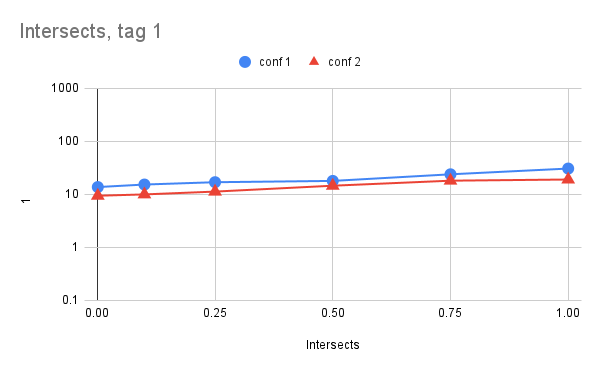
\includegraphics[width=\linewidth]{img/Intersects-tag-1.png}
    \caption{Syntetic workload, intersects, tag 1}\label{fig:intersects1}\par 
    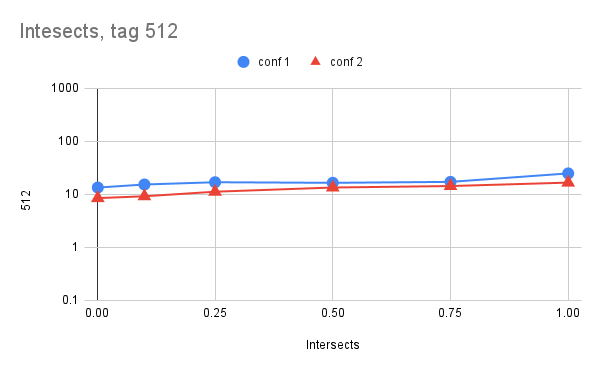
\includegraphics[width=\linewidth]{img/Intesects-tag-512.png}
    \caption{Syntetic workload, intersects, tag 512}\label{fig:intersects512}\par 
\end{multicols}
\begin{multicols}{2}
    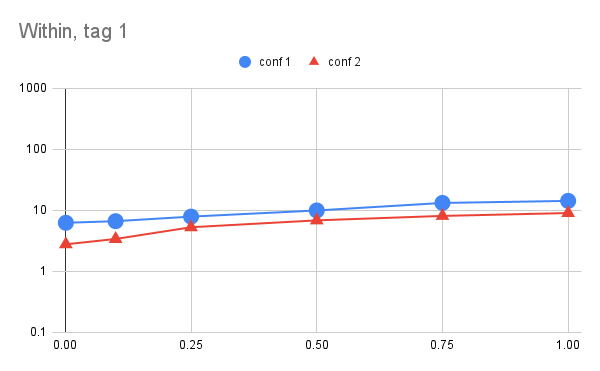
\includegraphics[width=\linewidth]{img/Within-tag-1.png}
    \caption{Syntetic workload, within, tag 1}\label{fig:within1}\par
    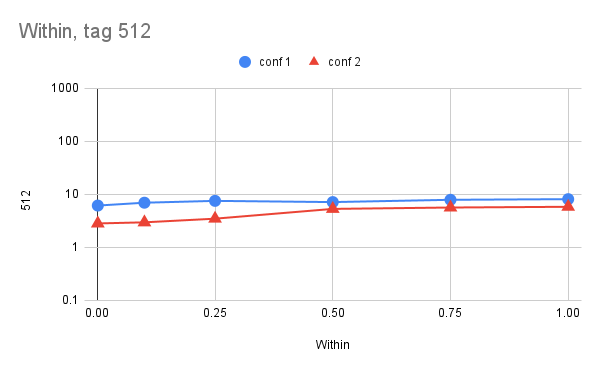
\includegraphics[width=\linewidth]{img/Within-tag-512.png}
    \caption{Syntetic workload, within, tag 512}\label{fig:within512}\par
\end{multicols}
\end{figure*}


The synthetic workload in Geographica 2 is designed using a generator that produces synthetic datasets of varying sizes, enabling the controlled evaluation of geospatial triplestores. This generator not only creates datasets with specific characteristics but also instantiates query templates that vary in both thematic and spatial selectivity. By doing so, Geographica 2 allows for a systematic examination of performance under different data and query conditions, from highly selective spatial queries to more comprehensive queries with minimal selectivity. 

This synthetic workload approach enables precise and repeatable performance assessments, ensuring that the evaluation of geospatial triplestores is not influenced by unpredictable real-world data variations. Through this controlled environment, researchers can measure the efficiency, scalability, and responsiveness of geospatial stores across a range of scenarios. This setup is invaluable for identifying performance trends and limitations that may be obscured in real-world datasets, making it possible to optimize triplestore configurations based on specific workload demands.

The \Cref{fig:intersects1,fig:intersects512,fig:within1,fig:within512} presented in this section illustrate response times for two configurations of GeoSPARQL Fuseki (conf 1 and conf 2) under various intersect and within conditions, where these configurations differ in their optimization settings. Analyzing the results, we observe a consistent trend where response times are influenced by both the proportion of matching features and the THEMA parameter value, with configuration 2 consistently outperforming configuration 1 across most cases.

For the `Intersects` predicate with THEMA set to 1, configuration 2 demonstrates superior efficiency, particularly as the query becomes more selective (e.g., filtering down to 0.01\% of the dataset features). This configuration shows a marked reduction in response time as the query specificity increases, reaching as low as 9.42 seconds for the most selective queries. This suggests that configuration 2 has optimizations that particularly benefit sparse spatial query results. In contrast, configuration 1, while generally slower, maintains steady performance across larger subsets (e.g., 50\% or more of dataset features), indicating its relative robustness in handling higher data loads.

When examining `Intersects` with THEMA set to 512, we observe similar patterns. Configuration 2 again outpaces configuration 1, achieving a response time as low as 8.5 seconds for the most selective cases (0.01\% of features). Notably, both configurations display a slight increase in response time when selecting 75\% or more of the dataset features, though configuration 2 remains more efficient under all proportions tested.

The `Within` predicate results show an even more pronounced efficiency for configuration 2. With THEMA at 1, configuration 2 achieves response times as low as 2.78 seconds for highly selective queries (0.01\% of features), a substantial improvement over configuration 1. For the `Within` predicate with THEMA set to 512, configuration 2 maintains similar advantages, particularly in selective queries, reaching response times as low as 2.83 seconds. Configuration 1 shows relatively steady performance here, but the times are consistently higher than those of configuration 2.

Overall, the data suggests that configuration 2 is well-suited for scenarios where high selectivity in spatial data queries is required, demonstrating reduced response times even in cases involving small feature subsets. In contrast, configuration 1 performs adequately in scenarios with broader data requirements, providing steady response times but lagging in more selective tasks. These findings highlight the flexibility and efficiency of GeoSPARQL Fuseki’s configurations in handling varied spatial query demands, emphasizing configuration 2’s advantage in optimized query processing for sparse result sets.

When comparing Fuseki's performance in the synthetic workload with its performance in real-world datasets, a clear trend emerges: the query response times in the synthetic workload exhibit a linear behavior within the range of $10^1$ seconds. This consistency across query types and dataset sizes suggests that Fuseki's optimizations are particularly effective under controlled conditions, as demonstrated in the synthetic workload generated by Geographica 2. 

In this context, Fuseki’s linear performance highlights its stability and scalability for geospatial queries, maintaining predictable response times even as the volume of queried features increases. The synthetic dataset’s controlled environment, with varying degrees of thematic and spatial selectivity, allows Fuseki to leverage indexing and optimization mechanisms effectively, thereby producing linear performance trends. In contrast, real-world datasets, with their inherent variability and less predictable distributions of geospatial features, may challenge triplestore optimizations in ways that deviate from this linear trend. 

This comparison underscores the efficiency of Fuseki in handling synthetic data, where controlled conditions allow it to deliver response times within a narrow and predictable range. Such performance insights are crucial for understanding Fuseki’s potential scalability and adaptability in varied environments and emphasize the importance of optimization in achieving consistent query response times across diverse geospatial workloads.


\section{Querying and Visualization}\label{VI-sec:querying}
The \textit{Querying} module serves as the final component of the framework, designed to facilitate user interaction with the knowledge graph, thereby transforming it into a dynamic, interactive tool for data exploration and analysis. This module offers sophisticated querying capabilities, particularly well-suited for handling complex geospatial data, and enables users to derive meaningful insights by directly engaging with the structure and content of the knowledge graph.


\subsection{Querying}\label{VI-subsec:querying}

At the core of this module’s functionality lies its proficient utilization of \acrshort{SPARQLLabel} \cite{ericprudhommeauxSPARQLQueryLanguage2008} and its querying capabilities, empowering users to execute complex queries that leverage geospatial relationships and extract data based on specific criteria. The module facilitates queries that traverse and interpret the rich semantic and geographic interconnections embedded in the knowledge graph. For instance, users can specify queries to retrieve all farms situated within a given radius of a water source or to identify regions contiguous to a particular city. These examples illustrate the ability to integrate both spatial and relational data, enabling the exploration of intricate geographic and topological relationships across varied datasets.

Moreover, the module extends beyond conventional querying by incorporating advanced geospatial functions through GeoSPARQL \cite{matthewperryOGCGeoSPARQLGeographic2012}. This integration empowers users to formulate spatial queries grounded in geographic features, such as exact coordinates or relative proximity to specified landmarks. By defining queries with detailed spatial parameters, users can enhance data retrieval processes to align with precise geospatial criteria. This capacity significantly broadens analytical possibilities, addressing questions that require a sophisticated understanding of spatial distribution, adjacency, and other complex geographic patterns.

Through the interplay of these functionalities, the Querying module offers a holistic and dynamic means of interacting with the knowledge graph. It provides a robust mechanism for \acrshort{SPARQLLabel}-based data retrieval while seamlessly integrating geospatial parameters and GeoSPARQL-driven queries, facilitating a multidimensional exploration of both relational and spatial aspects of the data. Consequently, the module transforms the knowledge graph into a powerful instrument for analyzing geospatial information, fostering deeper engagement and enabling a comprehensive exploration of geographic and topological insights.


\subsection{Visualization}\label{VI-subsec:visualization}

The visualization module in the framework utilizes the \acrfull{SMBVTLabel} module to render graphs as Story Maps, a concept introduced in \cite{bartalesiWebToolCreate2023c, bartalesiUnstructuredTextsSemantic2023b}. Story Maps are a visualization paradigm focused on presenting maps as dynamic narratives, where sequences of events are enriched with multimedia elements to create an engaging, spatially structured storytelling experience. Many software solutions exist for creating and visualizing story maps, with a focus on platforms that enable users to integrate text, images, audio, and video. These platforms aim to produce interactive, map-based narratives that guide users through immersive storytelling paths.

ArcGIS StoryMap is one of the foremost platforms in this area, known for its flexibility in designing, publishing, and sharing interactive story maps \cite{walsheUsingArcGISOnline2016}. This software allows for a high degree of customization, permitting users to augment their narrative flow through the incorporation of diverse multimedia elements. Although ArcGIS StoryMap offers an array of commercial versions with expanded features, a free version is also available. However, the free version comes with several restrictions: it lacks support for embedding external web pages, limits advanced map interaction capabilities, and reduces options for theme customization. Accessibility settings are similarly constrained, and perhaps most notably, the free version does not support integration with entities from existing knowledge bases such as Wikidata.\footnote{These limitations in the free version reflect typical restrictions in proprietary storytelling platforms, which may constrain the degree of interactivity and linkage to external datasets.}

In contrast, Timescape is another map-based storytelling tool that allows users to enrich events with text, images, and external links \cite{Timescape}. Like ArcGIS, Timescape is a commercial product, although a free tier allows for the creation of up to five story maps. A distinctly different tool, StoryMapJS, offers a fully free option accessible online or as a JavaScript library \cite{knightlabStoryMapJS}. StoryMapJS organizes stories through a sequence of slides, each depicting an event tied to a specific location, and enables users to link multimedia content to these events. By leveraging Google accounts for editor access, StoryMapJS serves as a versatile tool for digital storytelling, albeit without some of the advanced customization options found in ArcGIS.

For users with web development experience, constructing story maps through custom HTML templates offers another viable method. An example is the Leaflet Storymaps template, which guides readers through a point-by-point narrative while integrating scrolling features to enhance engagement \cite{sveenAtlefrenStorymap2024}. This template provides options for embedding multimedia, such as images, audio, video, and scanned map backgrounds, with map data entered through connected Google Sheets or CSV files. The HTML template approach allows for a high degree of customization, though it requires a more significant initial setup and a greater technical proficiency.

Open-source tools like Odyssey.js present hybrid approaches to story map creation. Odyssey.js allows users to create story maps using Markdown, with a limited number of webpage templates to expedite the creation process \cite{Odysseyjs}. This combination of HTML coding and external data structuring provides some flexibility, although it requires a certain level of technical skill and may lack the seamless integration features found in more advanced platforms.

Despite their utility in building story maps, these tools exhibit significant limitations compared to the SMBVT module, particularly in their handling of semantic integration and story inter-linking. Unlike the software reviewed, SMBVT leverages Semantic Web technologies, enabling it to link seamlessly with structured knowledge bases like Wikidata, thereby supporting enhanced data integration and interconnectivity between stories. SMBVT’s fully free availability further distinguishes it by removing the access and functionality constraints often inherent in both commercial and open-source alternatives. This unique combination of semantic linking and accessibility establishes SMBVT as an innovative tool in the field of story map creation, effectively addressing the common drawbacks of existing platforms and equipping users with a powerful solution for creating semantically enriched story maps.



% \section{Integration of Case Studies}

% The framework has been applied to datasets from the \textit{MOVING} and \textit{IMAGO} projects, each of which provided unique challenges for geospatial data representation and reasoning. Through the framework, these datasets were transformed into enriched knowledge graphs that support advanced geospatial queries and reasoning.

% For the \textit{MOVING} project, the framework handled agricultural data, such as farm locations, crop yields, and environmental factors. The \textit{IMAGO} project, on the other hand, dealt with geographic narratives, requiring the framework to capture complex spatial relationships between historical events and geographic features.

\section{Conclusion}

The architecture of the NOnt+S evaluation framework provides a robust, modular system for processing, analyzing, and visualizing geospatial data. By integrating modules for linking, representation, reasoning, storage, and querying, the framework enables the creation of a dynamic geospatial knowledge graph. This architecture supports interdisciplinary research, providing valuable insights into both agricultural and geographic domains through its advanced semantic capabilities.
 

\chapter{NOnt+S Evaluation and Data Validation}\label{chap:evaluation}

\section{Introduction}\label{VII-sec:introduction}

In this chapter, we present the evaluation and data validation of the NOnt+S ontology in two distinct scientific domains: bioeconomy studies and geographic medieval literature. This interdisciplinary evaluation was conducted within the scope of two projects: the \acrshort{MOVINGLabel} European project (Horizon 2020-2024), focused on the bioeconomy, and the \acrshort{IMAGOLabel} Italian project (PRIN 2020-2024), centered on geographic literature. The primary goal of this chapter is to illustrate the practical application of the Semantic Web framework, which was introduced in the preceding \Cref{chap:SW-framework}, and demonstrate how it was applied to assess and validate the NOnt+S ontology across these two scientific domains.

By evaluating the NOnt+S ontology in both bioeconomy and geographic research, we aim to validate its robustness, flexibility, and capacity to provide comprehensive models that can be applied in different research areas. The interdisciplinary nature of this validation is crucial in assessing the ontology’s adaptability and its ability to model complex, domain-specific knowledge. 

\section{Methodology}\label{VII-sec:methodology}

The methodology employed for the evaluation and validation of the NOnt+S ontology is grounded in the framework described in the \Cref{chap:SW-framework}. This framework establishes a systematic approach to develop a semantic web framework. The evaluation is assessed through a combination of metrics and qualitative parameters, including:

\begin{itemize}
    \item \textbf{Linking and Enhancement}: Ensuring the linking and enrichment of the data, provided by the module linking and enhancement.
    \item \textbf{Representational Power}: Evaluating how well the ontology represents all relevant concepts within the target domain and ensures comprehensive coverage of the necessary information.
    \item \textbf{Consistency}: Ensuring logical consistency of the ontology, provided by the Reasoner module of the framework
    \item \textbf{Querying}: data validation was performed through the implementation of \acrshort{SPARQLLabel}/GeoSPARQL queries to ensure the alignment of data with the defined ontology structure.
    \item \textbf{Reusability}: Measuring the potential for the ontology to be adapted for use in related but distinct domains.
    
\end{itemize}

\section{Bioeconomy Studies: MOVING Project (2020-2024)}\label{VII-sec:moving}

The \acrfull{MOVINGLabel} project\cite{MOVINGHorizon2020} is a European Union Horizon 2020 initiative focused on fostering the sustainability and resilience of mountain regions. This project focuses on mountain \acrfullpl{VCLabel} and their capacity to adapt to climate and societal shifts. The project aims to develop value chains that enhance the socio-economic viability of these regions while promoting environmental sustainability. By creating a European-wide Community of Practice (CoP), \acrshort{MOVINGLabel} facilitates collaboration between stakeholders, including policymakers, researchers, and businesses. The project involves assessing and benchmarking value chains to identify key enablers and barriers to sustainability. Furthermore, it seeks to anticipate future trends affecting mountain territories through foresight exercises and policy roadmaps.

The \acrshort{MOVINGLabel} project is directly relevant to this research because its dataset, which includes geospatial data related to mountain regions, is used to test the NOnt+S developed for geospatial representation. By enriching this data with semantic knowledge, the project’s findings contribute significantly to the research on querying, inferring, and visualizing geographic information within narratives. This integration of geospatial knowledge aids in improving the tools and methodologies for representing and analyzing complex geographic information in digital libraries.

The data we elaborated were provided by territorial experts involved in the \acrshort{MOVINGLabel} European project. By utilizing a bottom-up participatory approach, \acrshort{MOVINGLabel} gathers data and develops strategies to address these changes while evaluating the present state of European mountain ecosystems, cultural heritage, and societies. Sixteen experts from sixteen different European countries contributed to the project, supplying a total of 454 documents, each detailing a specific VC. These documents covered a wide range of aspects, including economic, climatic, historical, ecological, cultural, territorial, and societal dimensions. The information within the documents focused on the natural characteristics of \acrshort{VCLabel} territories, quantitative data such as geography, population, income, tourism, and employment figures, as well as the key regional products and associated value chains.

Following the methodology outlined in \Cref{chap:methodology}, we created narratives composed of events. A fundamental step in this process is the geospatial enrichment of the data included in the dataset, such as \acrfullpl{LAULabel}. In this phase of the research, we enriched the dataset by retrieving additional geospatial information from external sources, such as the \acrfull{GISCOLabel}\cite{GISCOEurostat} and \acrfull{OSMLabel}\cite{OpenStreetMap}. This enrichment process resulted in a more detailed and comprehensive dataset. Then the knowledge have been represented using the NOnt+S ontology and stored in the Triple store after the creation of a knowledge graph consisting of 503,963 triples to represent and query agricultural geospatial data. One of the key elements of this phase was the use of GeoSPARQL, a specialized query language for geospatial data. The use of GeoSPARQL enabled advanced queries, allowing us to identify spatial trends in agricultural practices across the dataset. These insights proved valuable for understanding the spatial relationships between agricultural practices and geographic locations, helping to optimize land use and inform policy decisions.

\subsection{Geospatial Enrichment}\label{VII-subsec:geospatialEnrichment}
To enrich the narrative datasets with geospatial knowledge, an algorithm composed by two modules were developed. These algorithm automate the process of extracting geospatial information from external sources and integrating it into the knowledge base.

\subsubsection{Extraction from GISCO}\label{VII-subsubsec:gisco}
The first module focuses on extracting the geometry of \acrshortpl{LAULabel} from the \acrshort{GISCOLabel} datasets. This process involves matching the \acrshortpl{LAULabel} reported as textual strings in the narrative datasets with their corresponding geospatial coordinates in \acrshort{GISCOLabel}. The output is a set of polygons or points that represent the \acrshortpl{LAULabel} in geographic space.


\begin{algorithm}[H]
\caption{Data Augmentation Algorithm - LAU/NUTS Geometry Extraction}
\label{alg:gisco}
\SetAlgoLined
\KwData{VC Event Table with LAU or NUTS Codes}
\KwResult{VC Table Augmented with WKT Geometries}
\For{each event}{
    Extract the country code from the member state description\;
    Extract the LAU code\;
    Check if the code-country pair exists in the GeoJSON LAU GISCO file\;
    \If{a match is not found}{
        Check if the code-country pair exists in the GeoJSON NUTS GISCO file\;
    }
    \If{a match is found}{
        Extract the WKT-polygon representation\;
        Save the WKT polygon in the geometry column (with LAU/NUTS label)\;
    }
}
\end{algorithm}

The module 1 is described in \Cref{alg:gisco}\footnote{The code of the module is available on GitHub at \url{https://github.com/prate91/LAU_extraction}}. It is designed to augment a dataset of events, referred to as the \acrshort{VCLabel} Event Table. The table contains one event for each rows, which contains \acrshortpl{LAULabel} or \acrfull{NUTSLabel} codes. The goal is to enrich this table by associating each event with its corresponding geographical geometry in the form of \acrshort{WKTLabel} polygonal representations.

The algorithm illustrated in \Cref{fig:alg1} begins by iterating over each event in the \acrshort{VCLabel} Event Table. For each event, the country code is first extracted from the event's member state description. Alongside this, the LAU code is extracted from the event itself. With the combination of the LAU code and country code, the algorithm proceeds to verify whether this pair exists in a pre-defined GeoJSON LAU GISCO file, which contains the geographical boundaries of administrative units across countries in a format suitable for spatial data.

\begin{figure}
\begin{tikzpicture} [
    auto,
    decision/.style = { diamond, draw=blue, thick, fill=blue!20,
                        text width=8em, text badly centered,
                        inner sep=1pt, rounded corners },
    block/.style    = { rectangle, draw=blue, thick, 
                        fill=blue!20, text width=10em, text centered,
                        rounded corners, minimum height=2em },
    line/.style     = { draw, thick, ->, shorten >=2pt },
  ]
  % Define nodes in a matrix
  \matrix [column sep=5mm, row sep=10mm] {
                    & \node [text centered] (e) {$\forall e_i \in E$};            & \\
                    & \node (null1) {};                                    & \\
                    & \node [block] (ExCTR) {\textsf{ExCTR}($e_i$)};   & \\
                    & \node [block] (ExLAU) {\textsf{ExLAU}($e_i$)};   & \\
    \node(null3){}; & \node [decision] (giscolau)
                        {\textsf{GSCL($cd,ctr$,\textsf{GL})}};
                                  & \node[text centered](glau){\textsf{GL}}; \\
    \node(null4){}; & \node [decision] (gisconuts)
                        {\textsf{GSCN($cd,ctr$,\textsf{GN})}};
                                  & \node[text centered](gnuts){\textsf{GN}}; \\
                    & \node [block] (track) {\textsf{WKT}(GL) or \textsf{WKT}(GN)}; & \\
                    % & \node [block] (track2) {\textsf{WKT}($j$)}; & \\
                    & \node [block] (pesos)
                        {\textsf{ADD}(WKT,$e_i$)};            & \\
                    & \node [block] (iterate)
                        {\textsf{ITERATE}};          & \\
                    & \node [text centered] (end) {end};          & \\
  };
  % connect all nodes defined above
  \begin{scope} [every path/.style=line]
    \path (e)        --    (ExCTR);
    \path (ExCTR)    --    node [near start] {$e_i, ctr$} (ExLAU);
    \path (ExLAU)      --    node [near start] {$ctr, cd$} (giscolau);
    \path (glau)      --    (giscolau);
    \path (gnuts)      --    (gisconuts);
    \path (giscolau)      --    node [near start] {no} (gisconuts);
    \path (giscolau)   --++  (-4,0) node [near start] {yes} |- (track);
    \path (gisconuts)   --++  (-3,0) node [near start] {no} |- (e);
    \path (gisconuts)   --  node [near start] {yes} (track);
    \path (track)    --    node [near start] {\textsf{WKT}} (pesos);
    \path (pesos)    --   (iterate);
    \path (iterate)   --++  (-5,0) node [near start] {$i$} |- (e);
    \path (iterate) --    (end);
  \end{scope}
  %
  % legend for subprocedures
  \node (leyend) at (7, 6){
    \begin{tabular}{>{\sffamily}l@{: }l}
      \multicolumn{2}{c}{\textbf{subprocedures}} \\
      ExCTR & extract country from event $e_i$     \\
      ExLAU  & extract LAU from event $e_i$      \\
      GSCL & search code $cd$ in  GISCO LAUs (GL)                    \\
      GSCN   & search code $cd$ in GISCO NUTS (GN)                        \\
      WKT   & extract WKT from GISCO LAUs or NUTS \\
      ADD   & add WKT to event $e_i$
    \end{tabular}
  };
  %
  % legend for input and output variables
  \node (leyend) at (7, 0){
    \begin{tabular}{l@{: }l}
      \multicolumn{2}{c}{\textbf{variables}}              \\
      $\mathbf{E},\,\mathbf{e_i}$ & events           \\
      $cd$                       & LAU or NUTS code candidate  \\
      $ctr$              & country code \\
      WKT               & WKT geometry    \\
      GL        & GISCO LAU code         \\
      GN              & GISCO NUTS code
      \end{tabular}
  };
\end{tikzpicture}
\caption{This diagram illustrates Module 1 of the algorithm for geospatial enrichment.}
\label{fig:alg1}
\end{figure}


If the LAU code-country pair is not found in the LAU GISCO file, the algorithm attempts a secondary search in the GeoJSON NUTS GISCO file. This file contains higher-level territorial divisions (NUTS codes), which can serve as an alternative if the LAU-level data is unavailable or unmatched.

Once a match is identified in either the LAU or NUTS GISCO file, the algorithm extracts the geographical information for that region in the form of a WKT-polygon. This polygon is a text representation of the region's boundaries, expressed in a standard markup language for vector geometry objects.

Finally, the WKT-polygon is stored in the \acrshort{VCLabel}Event Table, in a new column designated for geometry data. This column also labels whether the geometry corresponds to an LAU or NUTS code, ensuring clarity in the augmented table. By the end of this process, each event in the \acrshort{VCLabel}Event Table is enriched with its corresponding geographical geometry, making the dataset more comprehensive for spatial analysis.


\subsubsection{Extraction from \acrshort{OSMLabel} and Wikidata}\label{VII-subsubsec:osm-wikidata}
The second module extracts the geometries of natural and administrative places cited in the narrative datasets from OpenStreetMap. Using QLever, an OSM endpoint, the correct geometry of each place is identified. In addition to geometric data, the corresponding Wikidata entities are also retrieved, linking the geographic places with structured semantic information.

\begin{algorithm}[H]
\caption{Data Augmentation Algorithm - Named Entity Extraction}
\label{alg:entityextraction}
\SetAlgoLined
\KwData{Event Description and Title}
\KwResult{List of Named Entities with Associated Coordinates and Geometries}
\For{each event description and title}{
    Invoke the NLPHub to extract all \emph{location}, \emph{person}, and \emph{organisation} named entities, as well as the \emph{keywords}\;
    \For{each extracted named entity}{
        Check validity (i.e., no ambiguity exists) with respect to Wikidata/Wikipedia entries\;
        \If{the entity is of \emph{location} type}{
            Try to retrieve the associated latitude and longitude coordinates from the Wikidata entry\;
            Retrieve the polygonal geometry using the external QLever \acrshort{SPARQLLabel} server of University of Freiburg\;
        }
    }
    Collect the list of entities and coordinates associated with the event\;
}
\end{algorithm}

The module 2 is described in \Cref{alg:entityextraction}\footnote{The code of the module is available on GitHub at \url{https://github.com/prate91/LAU_extraction}}. It aims to enhance event data by identifying and extracting named entities from the event's description and title. The algorithm focuses on extracting location, person, and organization entities, along with keywords, and associates relevant spatial information when applicable. It produces a list of named entities enriched with coordinates and geometries, if available.

 The process illustrated in \Cref{fig:alg2} begins by iterating over the dataset, where each event's description and title are analyzed. Using the \textit{NLPHub}\cite{coro2021nlphub}, the algorithm extracts the relevant entities, specifically identifying those of \emph{location}, \emph{person}, and \emph{organization} types, in addition to extracting \emph{keywords}. These entities are directly derived from the textual data provided by the event's description and title.

Following the extraction process, each identified named entity is checked for its validity. This validation is performed by cross-referencing the entity against known entries in \textit{Wikidata} or \textit{Wikipedia}, ensuring that the entity is unambiguous. If ambiguity is detected, the entity is disregarded, thereby preventing erroneous matches or associations within the dataset.

For entities classified as \emph{locations}, the algorithm proceeds to further enrich the data by retrieving their corresponding geographical information. Initially, the latitude and longitude coordinates are retrieved from the entity's associated Wikidata entry. Once the coordinates are obtained, the algorithm queries the external \textit{QLever \acrshort{SPARQLLabel} server} from the University of Freiburg to retrieve the polygonal geometry for the location. To this aim, it used an instance of the open-access QLever endpoint of the University of Freiburg \cite{qleverinstance2024} to retrieve a possible polygon representation from the \acrshort{OSMLabel} subgraph included in this large knowledge graph. QLever is a \acrshort{SPARQLLabel} engine capable of efficiently indexing and querying large knowledge graphs (even with over 100 billion triples) such as Wikidata, Wikimedia Commons, \acrshort{OSMLabel}, UniProt, PubChem, and DBLP \cite{bast2017qlever}. The University of Freiburg populated a large knowledge graph with these sources. Our process reported all geometries found on the QLever service as \acrshort{WKTLabel} formatted strings\cite{WellknownTextRepresentationa}. This provides not only the geographical point (latitude and longitude) but also the spatial boundaries that describe the extent of the location in question.



\begin{figure}
\begin{tikzpicture} [
    auto,
    decision/.style = { diamond, draw=blue, thick, fill=blue!20,
                        text width=5em, text badly centered,
                        inner sep=1pt, rounded corners },
    block/.style    = { rectangle, draw=blue, thick, 
                        fill=blue!20, text width=10em, text centered,
                        rounded corners, minimum height=2em },
    line/.style     = { draw, thick, ->, shorten >=2pt },
  ]
  \matrix [column sep=5mm, row sep=10mm] {
                    & \node [text centered] (e) {$\forall e_i \in E$};            & \\
                    & \node (null1) {};                                    & \\
                    & \node [block] (nlphub) {$\textsf{NER}_{\textsf{NLPHub}}$($t(e_i), d(e_i)$)};   & \\
                    & \node [block] (validity) {\textsf{CV}($x_i$)};   & \\
    % \node(null3){}; & \node [decision] (valid) {\textsf{CV}($\mathbf{x}$} \\
    \node(null4){}; & \node [decision] (islocation)  {\textsf{is location?}};\\
                    & \node [block] (wiki) {\textsf{WD}(lat($x_i$),long($x_i$))}; & 
                    & \node [block] (qlever) {\textsf{QLev}($x_i$)};            & \\
                    & \node [text centered] (xf) {end};          & \\
  };
  % connect all nodes defined above
  \begin{scope} [every path/.style=line]
    \path (e)        --    (nlphub);
    \path (nlphub)    --    node [near start] {$\forall x_i \in X$} (validity);
    \path (validity)      --     node [near start] {$\mathbf{x_i}$} (islocation);
    % \path (gnuts)      --    (gisconuts);
    \path (islocation)      --    node [near start] {yes} (wiki);
    \path (islocation)   --++  (-4,0) node [near start] {no} |- (xf);
    % \path (gisconuts)   --++  (-3,0) node [near start] {no} |- (e);
    % \path (gisconuts)   --  node [near start] {yes} (track);
    \path (islocation)    --    node [near start] {yes} (qlever);
    % \path (pesos)    --    node [near start] {\textbf{w}} (filtrado);
    \path (wiki) --    (xf);
    \path (qlever) --    (xf);
  \end{scope}
  %
  % legend for subprocedures
  \node (leyend) at (3, 5){
    \begin{tabular}{>{\sffamily}l@{: }l}
      \multicolumn{2}{c}{\textbf{subprocedures}} \\
      % NLPHub & extract named entities     \\
      $\textsf{NER}_{\textsf{NLPHub}}$  & extract location, person, organisation  \\
      CV & check Wikidata validity of entity $x_i$ \\
      WD   & retrieve latitude, longitude from Wikidata  \\
      QLev   & retrieve polygon geometry from QLever
    \end{tabular}
  };
  %
  % legend for input and output variables
  \node (leyend) at (4, 0){
    \begin{tabular}{l@{: }l}
      \multicolumn{2}{c}{\textbf{variables}}              \\
      $E,e_i$ & events            \\
      $X, x_i$ & entities            \\
      $t(e_i)$                      & title of the event    \\
      $d(e_i)$              & description of the event \\
      
      \end{tabular}
  };
\end{tikzpicture}
\caption{This diagram illustrates Module 2 of the algorithm for geospatial enrichment.}
\label{fig:alg2}
\end{figure}

Once all named entities have been extracted, validated, and enriched, the algorithm aggregates them into a list associated with the specific event. For location-type entities, this list includes the coordinates and geometrical boundaries, where available. This augmentation process thus transforms the event data by adding precise spatial information and detailed named entity references, making the data more suitable for further spatial and analytical tasks.

\subsection{Knowledge Graph Creation and Storage}\label{VII-subsec:moving-kg}
Following the framework outlined in the thesis, the knowledge graph\footnote{The graph can be downloaded at \url{https://geosparql.isti.cnr.it/ontology/moving.owl}} was created using the triplifier module based on the NOnt+S representational model. This model adheres to \acrshort{OWLLabel} 2 DL \cite{OWLWebOntologyc} standards, ensuring compatibility with various semantic web technologies. The triplifier module facilitated the transformation of enriched geospatial data, value chain information, and additional metadata into \acrshort{OWLLabel} triples, structured according to the ontology’s model. Each entity, such as geographical regions (e.g., \acrshortpl{LAULabel}, \acrshort{NUTSLabel}), environmental factors, and value chains, was linked to relevant properties and relationships, enabling detailed semantic representation.

In total, the graph contains over 503,963 triples, providing a robust foundation for semantic querying and knowledge discovery across the diverse datasets involved in the \acrshort{MOVINGLabel} project. 


\subsection{Consistency of the Knowledge Graph}\label{VII-subsec:moving-consistency}
Following the framework, to ensure the reliability and integrity of the knowledge graph, we employed Openllet\cite{galigatorGaligatorOpenllet2024} to verify its consistency. Openllet checks for logical errors, such as violations of class hierarchies, incorrect data property assertions, and inconsistencies in the relationships between individuals in the graph. Specifically, the reasoner was used to validate that all entities conformed to the domain and range restrictions defined in the NOnt+S ontology.

The consistency check ensured that no contradictory information was present in the graph and that all axioms defined in the ontology were respected. For instance, it verified that geographical entities had valid spatial relationships and that value chains were correctly associated with their respective locations and environmental conditions.

By running regular consistency checks during the development process, we ensured that the knowledge graph remained logically coherent and could be used confidently for advanced querying and decision support tasks.

\subsection{Requirement Analysis and Querying}\label{VII-subsec:moving-querying}
We verified that querying the knowledge graph could aid in discovering new knowledge from the data. In particular, we collected the types of queries that the \acrshort{MOVINGLabel}-project scientists or stakeholders considered valuable, specifically those that were difficult to address without the use of a semantic knowledge representation. These queries were gathered during plenary meetings with the \acrshort{MOVINGLabel} Community of Practice (CoP), through identifying the principal study targets of rural-area experts involved in the project, particularly focusing on the \acrshortpl{VCLabel} within their respective territories, and by reviewing project deliverables and reports.

The experts focused on identifying \acrshortpl{VCLabel} that shared common environmental characteristics (e.g., rivers, lakes, vineyards, and chestnut trees), common issues (e.g., depopulation, pollution, deforestation), and similar products (e.g., cow or sheep milk, cheese). These queries were important for revealing hidden patterns within the data that would otherwise be challenging to discern without a knowledge graph. For example, uncovering clusters of \acrshortpl{VCLabel} affected by deforestation in proximity to specific geographical features like rivers or lakes enabled researchers to analyze the relationships between environmental degradation and \acrshort{VCLabel} productivity.

Discovering such knowledge is crucial for mountain ecosystems, as it informs the development of sustainable environmental management strategies. By uncovering connections between environmental and socio-economic factors, the knowledge graph facilitated targeted interventions for maintaining the ecological sustainability of rural areas. Additionally, this knowledge aids in the long-term planning for urban-rural linkages and in understanding the decline of essential services in mountain regions—challenges exacerbated by ongoing depopulation trends.

Through our demonstration, we showed that the knowledge graph could significantly enhance decision-making in these areas, providing a deeper understanding of the challenges facing mountain regions and contributing to more sustainable practices in both rural and urban contexts.

We focussed on four types of knowledge-extraction targets, corresponding to four GeoSPARQL queries regarding different and complementary aspects of European mountain products and their related spatial distributions.  Furthermore, these queries contribute directly to addressing Research Question 2 (\ref{quote:rq2}), offering a methodological framework for extracting and analyzing key data patterns. In particular, we extracted the \acrshortpl{VCLabel} with the following characteristics:
\begin{enumerate}
    \item operating in the Carpathian Mountains (Q1)
    \item operating around Trento city (Italy) (Q2)
    \item operating in Norway (Q3)
    \item operating around long european rivers ($>500$km) (Q4)
\end{enumerate}

The information extracted by these queries overall covered the interests of the \acrshort{MOVINGLabel} community experts. It would have been hard, indeed, to extract the same information through the usual data representation and technology adopted by this scientific community. Based on the query results, we calculated the following standard performance measurements: 

\[
Precision = \frac{TP}{TP+FP}
\]
\[
Recall = \frac{TP}{TP+FN}
\]
\[
F1 = 2 \cdot \frac{Precision \cdot Recall}{(Precision+Recall)}
\]

The performance measurements presented in \Cref{tab:evaluationQueries} reveal that our knowledge graph achieved exemplary outcomes, with Precision, Recall, and F1 score consistently attaining the value of 1 across all evaluated cases. This remarkable uniformity underscores not only the robustness of our knowledge representation but also the effectiveness of our query design and execution. To ensure the reliability of these results\footnote{The visualization of the queries can be replicated via the web application accessible at \url{https://github.com/prate91/GeoSPARQL-queries-visualization-for-thesis}}, we verified the outcomes of each query through a manual inspection process. This comprehensive validation step confirmed the consistency and correctness of the queries' performance, affirming the reliability and accuracy of our approach. In what follows, we provide a detailed exposition of the individual queries and their corresponding outcomes, offering a thorough analysis that highlights the strengths and performance characteristics of our semantic framework.

The consistent achievement of perfect scores in precision, recall, and F1-score is a remarkable indicator of the accuracy and reliability of the evaluation process. The manual inspection process was conducted by a team of ten specialized individuals, each possessing a significant level of expertise relevant to the domain of the dataset under consideration. These individuals were selected based on their advanced qualifications and proven experience, ensuring a high level of accuracy and consistency in their judgments. Their expertise was pivotal in meticulously reviewing the results of the dataset and validating them against the outcomes generated by the system.

The validation process followed a structured and systematic approach. Initially, the results produced by the system queries were juxtaposed with the manually reviewed and counted outcomes. Each member of the team undertook a thorough examination of the dataset, manually identifying and categorizing the results. This step was critical in establishing a gold standard against which the system's outputs could be evaluated.

To ensure accuracy, the experts adhered to a set of predefined criteria during the validation phase. These criteria were specifically designed to evaluate the correctness of the system's results in terms of precision, recall, and F1-score. Precision was validated by confirming that all retrieved instances were indeed relevant, thereby eliminating false positives. Recall was assessed by verifying that all relevant instances were retrieved, ensuring no false negatives. Finally, the F1-score, being the harmonic mean of precision and recall, reflected the overall balance and effectiveness of the system in both retrieving all relevant results and excluding irrelevant ones.

Each expert conducted their analysis independently, thereby minimizing bias and enhancing the robustness of the validation process. Following the individual assessments, the results were cross-verified among the team members to identify and rectify any discrepancies. This collaborative effort reinforced the reliability of the manual inspection process and ensured that the final validated results were of the highest standard.

The rigorousness of this manual inspection process, coupled with the qualifications and meticulous efforts of the expert team, accounts for the consistent perfect scores achieved in precision, recall, and F1-score. The manual validation provided a reliable benchmark, confirming the exceptional performance of the system and demonstrating the efficacy of the methodology employed.

\begin{table}[H]
    \centering
        \caption{Precision, Recall, and F1 measurements of our queries.}
    \label{tab:evaluationQueries}
    \begin{tabular}{|l|l|l|l|}
    \hline
 Query & Precision & Recall & F1\\
\hline
        Q1 & 1 & 1 & 1\\ \hline
        Q2 & 1 & 1 & 1\\ \hline
        Q3 & 1 & 1 & 1 \\  \hline
        Q4 & 1 & 1 & 1 \\ \hline
    \end{tabular}
\end{table}

\subsubsection*{Q1 - Value chains operating inthe Carpathian Mountains}
In the following, we report the GeoSPARQL query corresponding to Q1. The results are displayed in \Cref{fig:carpathian}.

\begin{lstlisting}[caption=GeoSPARQL Query 1, label={lst:query1}]
PREFIX /*!\gls{rdfs}!*/ <http://www.w3.org/2000/01/rdf-schema#>
PREFIX /*!\gls{geof}!*/ <http://www.opengis.net/def/function/geosparql/> 
PREFIX /*!\gls{geo}!*/ <http://www.opengis.net/ont/geosparql#>
PREFIX /*!\gls{narra}!*/ <https://dlnarratives.eu/ontology#>
PREFIX /*!\gls{osm}!*/ <https://www.openstreetmap.org/>
PREFIX /*!\gls{wd}!*/ <http://www.wikidata.org/entity/>
PREFIX /*!\gls{osm2rdfkey}!*/ <https://osm2rdf.cs.uni-freiburg.de/rdf/key#>

SELECT ?nlabel ?clabel ?wktLau
WHERE {	
    ?narra narra:isAboutCountry ?country ;
           narra:isAboutLAU ?lau ;
    	      rdfs:label ?nlabel .
    ?country rdfs:label ?clabel .
    ?lau geo:hasGeometry ?glau .
    ?glau geo:asWKT ?wktLau . 
    { 
    	SELECT ?wkt WHERE {
        	SERVICE 
      		  <https://qlever.cs.uni-freiburg.de/api/osm-planet> { 
            	?osm_id osm2rdfkey:wikidata wd:Q1288 ;
                        geo:hasGeometry ?geometry .
                ?geometry geo:asWKT ?wkt .
        	} 
    	}
  	}
   FILTER(geof:sfIntersects(?wktLau,?wkt)).
}
\end{lstlisting}


The \Cref{lst:query1} retrieves the \acrshort{VCLabel} narrative titles, countries, and \acrshort{LAULabel} polygons that overlap a polygon representing the Carpathian Mountains region. A value chain's Local Administrative Units (LAUs) define the primary areas where the value chain (VC) operates (i.e., where it produces and sells products). The query internally accesses the QLever endpoint provided by the University of Freiburg (\Cref{VII-subsubsec:osm-wikidata}), specifically utilizing the OpenStreetMap subgraph to define the Carpathian Mountains as a polygonal region.

The \texttt{SELECT} statement at line 9 specifies the output variables: \texttt{?nlabel} (narrative title), \texttt{?clabel} (country name), and \texttt{?wktLau} (LAU geometry in \acrshort{WKTLabel} format). These variables are the focus of the query’s output. The \texttt{WHERE} clause, beginning at line 10, contains the conditions required for each result. The following graph patterns are used:
\begin{itemize}
    \item At line 12, the triple pattern \texttt{?narrative \gls{narra}isAboutLAU ?lau} links each narrative to its corresponding LAU.
    \item At line 15, the triple pattern \texttt{?lau \gls{geo}hasGeometry ?glau} retrieves the geometry associated with each LAU.
    \item At line 16, the triple pattern \texttt{?glau \gls{geo}asWKT ?wktLau} provides the \acrshort{WKTLabel} representation of the LAU geometry.
\end{itemize}

A nested \texttt{SELECT} clause, beginning at line 18, retrieves the \acrshort{WKTLabel} geometries (\texttt{?wkt}) of the Carpathian Mountains region under the following \texttt{WHERE} conditions:
\begin{itemize}
    \item The \texttt{SERVICE} keyword is used to access the external QLever endpoint at \url{https://qlever.cs.uni-freiburg.de/api/osm-planet}.
    \item The triple pattern at line 21, \texttt{?osm\_id \gls{osm2rdfkey}wikidata \gls{wd}Q1286}, retrieves the instance corresponding to the Wikidata entity \textit{Carpathian Mountains} (\gls{wd}Q1288).
    \item The triple pattern at line 22, \texttt{?osm\_id \gls{geo}geometry ?geometry}, retrieves the \acrshort{IRILabel} representing the geometry of \texttt{\gls{wd}Q1288} (Carpathian Mountains).
    \item The triple pattern at line 23, \texttt{?geometry \gls{geo}asWKT ?wkt}, retrieves the \acrshort{WKTLabel}representation of the Carpathian Mountains geometry.
\end{itemize}

A final \texttt{FILTER} clause at line 27 performs an intersection between the LAU and Carpathian Mountains geometries, retrieving all LAU polygons that intersect with the Carpathian Mountains region. The resulting set of \acrshortpl{LAULabel} can be imported into a \acrshort{GISLabel} visualizer and overlaid with the Carpathian reference region (\Cref{fig:carpathian}).

Expert evaluation confirmed that the \acrshortpl{LAULabel} retrieved by this query were accurate and complete, achieving perfect precision and recall (both values equal to 1). Consequently, the query is effective in retrieving region-specific value chains.

\begin{figure}[h!tb]
    \centerline {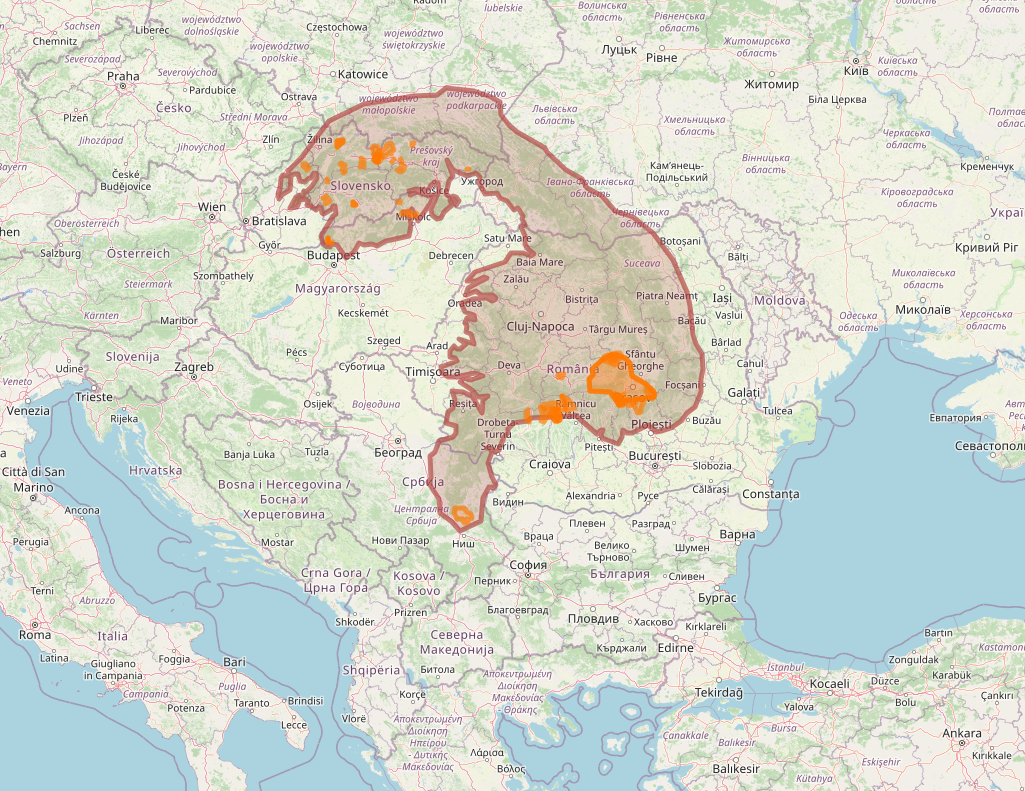
\includegraphics[scale=0.6]{img/carpathian.png}}
    \caption{Visualization of Q1}
    \label{fig:carpathian}
\end{figure}


\subsubsection*{Q2 - Value chains operating around Trento city (Italy)}
In the following, we report the GeoSPARQL query corresponding to Q2. The results are displayed in \Cref{fig:trento}.

\begin{lstlisting}[caption=GeoSPARQL Query 2, label={lst:query2}]
PREFIX /*!\gls{uom}!*/  <http://www.opengis.net/def/uom/OGC/1.0/>
PREFIX /*!\gls{rdfs}!*/  <http://www.w3.org/2000/01/rdf-schema#>
PREFIX /*!\gls{geof}!*/  <http://www.opengis.net/def/function/geosparql/> 
PREFIX /*!\gls{geo}!*/  <http://www.opengis.net/ont/geosparql#>
PREFIX /*!\gls{narra}!*/  <https://dlnarratives.eu/ontology#>
SELECT ?nlabel ?clabel ?wktLau
WHERE { 
       {
    ?narra narra:isAboutCountry ?country ;
            narra:isAboutLAU ?lau ;
            rdfs:label ?nlabel .
    ?country rdfs:label ?clabel .
    ?lau geo:hasGeometry ?glau .
    ?glau geo:asWKT ?wktLau .
}
    FILTER(geof:sfIntersects(
        ?wktLau,
        geof:buffer(
            "POINT(11.12108 46.06787)"^^geo:wktLiteral,
        0.5, uom:degree))). 
}
\end{lstlisting}

The \Cref{lst:query2} extracts the \acrshort{VCLabel}titles, countries and LAU geometries of the value chains operating within a maximum distance of 23 km from Trento. The query structure is similar to the one of Q1, with the difference that it does not use an external endpoint to retrieve the reference geometry. Instead, the FILTER clause operates an intersection between all \acrshortpl{VCLabel}' LAU geometries and a circular buffer of 0.3 degrees ($\sim$40 km) around the Trento longitude-latitude coordinates. 

The query produced the results visualised in \Cref{fig:trento}. As in the case of Q1, the expert's evaluation highlighted that the \acrshortpl{LAULabel} retrieved by this query were correct and complete (Precision and Recall were 1). Therefore, the query was valuable in retrieving city-specific \acrshortpl{VCLabel}.


\begin{figure}[h!tb]
    \centerline {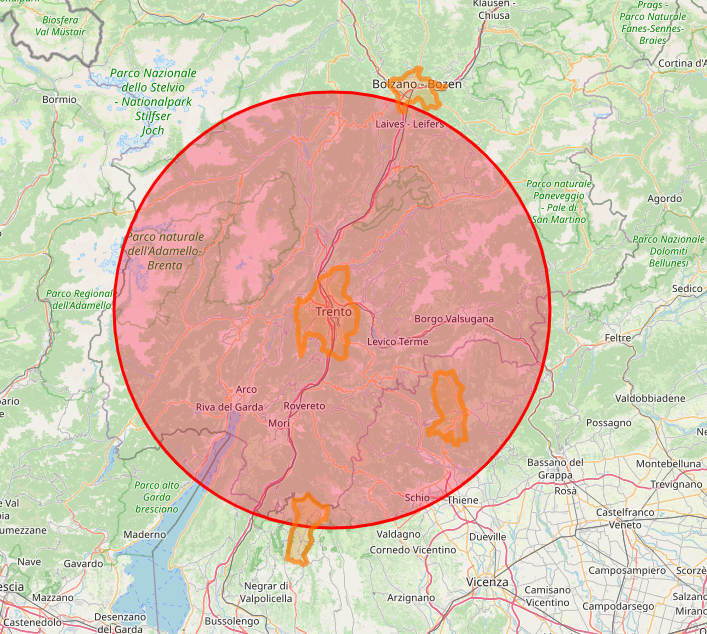
\includegraphics[scale=0.6]{img/trento.png}}
    \caption{Visualization of Q2}
    \label{fig:trento}
\end{figure}

\subsubsection*{Q3 - Value chains operating in Iberian Peninsula}
In the following, we report the GeoSPARQL query corresponding to Q3. The results are displayed in \Cref{fig:iberian}.

\begin{lstlisting}[caption=GeoSPARQL Query 3, label={lst:query3}]
PREFIX /*!\gls{uom}!*/ <http://www.opengis.net/def/uom/OGC/1.0/>
PREFIX /*!\gls{rdfs}!*/ <http://www.w3.org/2000/01/rdf-schema#>
PREFIX /*!\gls{geof}!*/ <http://www.opengis.net/def/function/geosparql/> 
PREFIX /*!\gls{geo}!*/ <http://www.opengis.net/ont/geosparql#>
PREFIX /*!\gls{narra}!*/ <https://dlnarratives.eu/ontology#>
PREFIX /*!\gls{osm}!*/ <https://www.openstreetmap.org/>
PREFIX /*!\gls{wd}!*/  <http://www.wikidata.org/entity/>
PREFIX /*!\gls{osm2rdfkey}!*/ <https://osm2rdf.cs.uni-freiburg.de/rdf/key#>

SELECT ?nlabel ?clabel ?wktLau 
WHERE  
    {   
        ?narra narra:isAboutCountry ?country ;
           narra:isAboutLAU ?lau ;
    	      rdfs:label ?nlabel .
    ?country rdfs:label ?clabel .
    ?lau geo:hasGeometry ?glau .
    ?glau geo:asWKT ?wktLau .
   { SELECT ?wkt WHERE {
        	SERVICE 
      		  <https://qlever.cs.uni-freiburg.de/api/osm-planet> { 
            	?osm_id osm2rdfkey:wikidata wd:Q12837 ;
                        a osm:relation ;
                        geo:hasGeometry ?geometry .
                ?geometry geo:asWKT ?wkt .
                
        	} 
    	} LIMIT 1
  	}
     FILTER(geof:sfWithin(?wktLau,?wkt)). 
}
\end{lstlisting}

The \Cref{lst:query3} extracts the \acrshort{VCLabel}titles, countries, and LAU geometries of the value chains operating in Scotland. The query structure is still similar to that of Q1. It uses the same external QLever Open Street Map endpoint to retrieve the geometry of Iberian Peninsula boundaries. The \texttt{FILTER} clause operates the intersection between Iberian Peninsula and the \acrshortpl{VCLabel}' LAU geometries. 

The query produced the results reported in \Cref{fig:iberian}. The expert's evaluation highlighted that the \acrshortpl{LAULabel} this query retrieved were correct and complete (Precision and Recall were 1). Therefore, the query was valuable in retrieving country-specific \acrshortpl{VCLabel}.


\begin{figure}[h!tb]
    \centerline {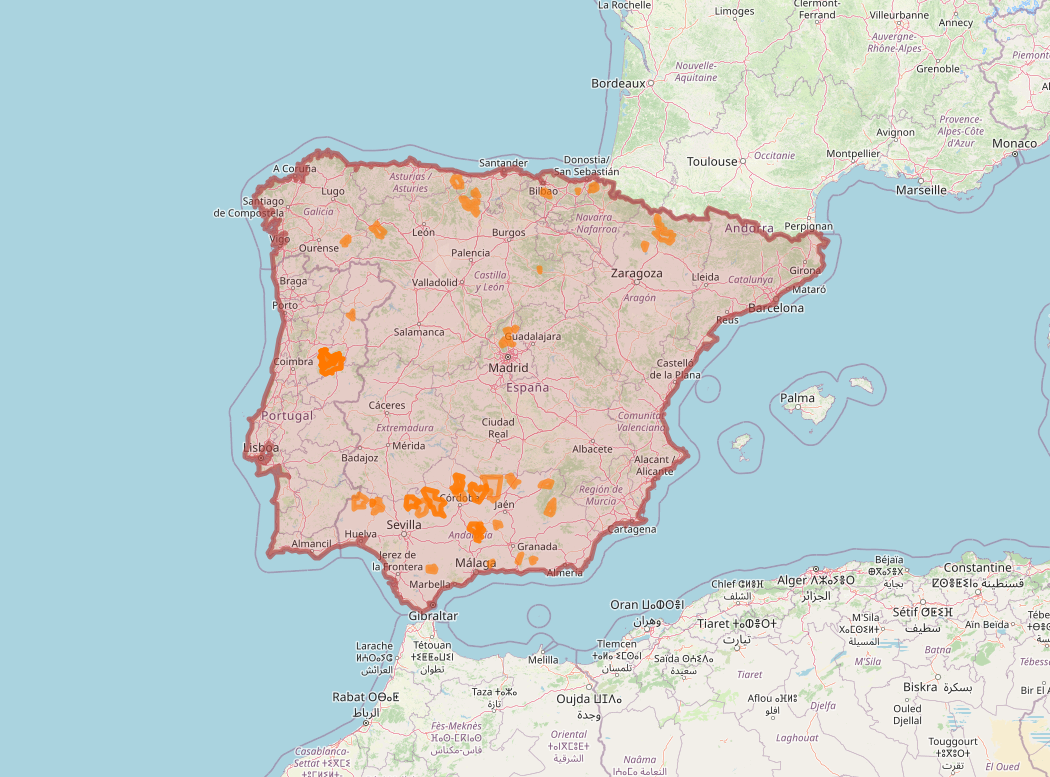
\includegraphics[scale=0.6]{img/iberian.png}}
    \caption{Visualization of Q3}
    \label{fig:iberian}
\end{figure}

\subsubsection{Q4 - Value chains operating around long European rivers}
In the following, we report the GeoSPARQL query corresponding to Q4. The results are displayed in \Cref{fig:rivers}.

\begin{lstlisting}[caption=GeoSPARQL Query 4, label={lst:query4}]
PREFIX /*!\gls{osmkey}!*/ <https://www.openstreetmap.org/wiki/Key:>
PREFIX /*!\gls{wd}!*/ <http://www.wikidata.org/entity/>
PREFIX /*!\gls{osm}!*/ <https://www.openstreetmap.org/>
PREFIX /*!\gls{wdt}!*/ <http://www.wikidata.org/prop/direct/>
PREFIX /*!\gls{uom}!*/ <http://www.opengis.net/def/uom/OGC/1.0/>
PREFIX /*!\gls{rdfs}!*/ <http://www.w3.org/2000/01/rdf-schema#>
PREFIX /*!\gls{geof}!*/ <http://www.opengis.net/def/function/geosparql/> 
PREFIX /*!\gls{geo}!*/ <http://www.opengis.net/ont/geosparql#>
PREFIX /*!\gls{narra}!*/ <https://dlnarratives.eu/ontology#>
PREFIX /*!\gls{osm2rdfkey}!*/ <https://osm2rdf.cs.uni-freiburg.de/rdf/key#>

SELECT ?nlabel ?clabel ?wktLau 
WHERE { 
    ?narra narra:isAboutCountry ?country ;
            narra:isAboutLAU ?lau ;
            rdfs:label ?nlabel .
    ?country rdfs:label ?clabel .
    ?lau geo:hasGeometry ?glau .
    ?glau geo:asWKT ?wktLau .
{
SELECT DISTINCT ?river_osm ?river_wd ?river_name ?length ?wkt WHERE {
    SERVICE <https://qlever.cs.uni-freiburg.de/api/osm-planet> {
        ?river_osm a osm:relation ;
                osmkey:waterway ?waterway ;
                geo:hasGeometry ?geometry ;
                osmkey:name ?river_name ;
                osm2rdfkey:wikidata ?river_wd .
        ?geometry geo:asWKT ?wkt .
    SERVICE <https://qlever.cs.uni-freiburg.de/api/wikidata> {
        ?river_wd wdt:P31/wdt:P279* wd:Q4022 ;
                wdt:P30 wd:Q46 ;
                wdt:P2043 ?length .
        FILTER (?length > 500)
    }
    }
} ORDER BY DESC(?length) 
}
FILTER(geof:sfIntersects(?wktLau, ?wkt)). 
}

\end{lstlisting}

The \Cref{lst:query4} retrieves all \acrshortpl{VCLabel} operating close to a European river longer than 500 km. The query structure is very similar to that of Q1 and uses the same external endpoint. The main differences are the following:
\begin{itemize}
    \item the nested \texttt{SELECT} clause operates on two different QLever-instance subgraphs: Open Street Map and Wikidata. The query retrieves the river geometries from the first. Then it uses the second to retrieve the list of "rivers" (\gls{wd}Q4022) present in "Italy" (\gls{wd}Q46) whose "length" (id. P2043) exceeds 500km ("FILTER (?length > 500)"); 
    \item the final \texttt{FILTER} clause operates the intersection between the Italian rivers and the \acrshortpl{VCLabel}' LAU geometries. 
\end{itemize}

The query produced the results reported in \Cref{fig:rivers}. All \acrshortpl{VCLabel} retrieved were correct and complete (Precision and Recall were 1). Therefore, the query was valuable in retrieving river-related \acrshortpl{VCLabel} and, by extension, could be used to extract water-basin-related \acrshortpl{VCLabel}.

\begin{figure}[h!tb]
    \centerline {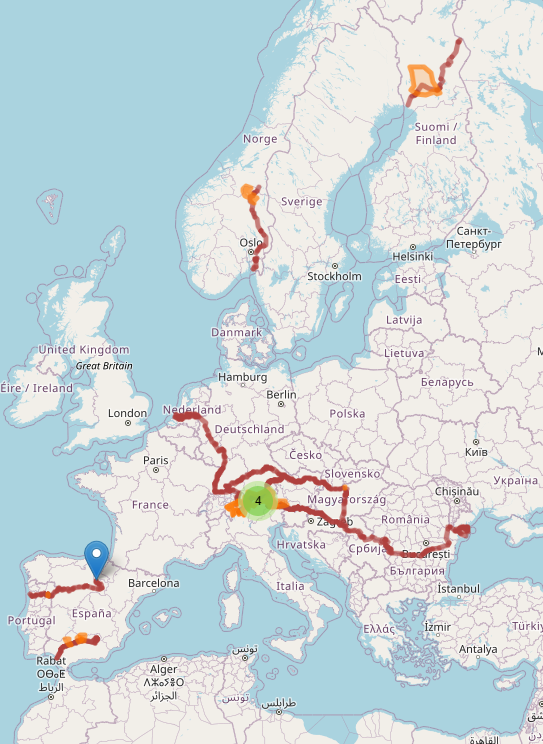
\includegraphics[scale=0.6]{img/rivers.png}}
    \caption{Visualization of Q4}
    \label{fig:rivers}
\end{figure}


\subsection{Visualization: Story Maps}\label{VII-subsec:moving-visualization}

Story maps are tools for visualizing narratives by embedding story events in spatial contexts. To visualize the 454 VC, we used a module of the Storymaps Building and Visualizing Tool (SMBVT) \cite{bartalesiWebToolCreate2023b}, which allows narratives to be mapped interactively, enhancing user engagement and understanding through multimedia and spatial linking. SMBVT employs Storymap.js \cite{zhaoJakobzhaoStorymap2024}, a JavaScript library for creating interactive map-based stories, which has been customized to meet the specific needs of SMBVT’s narrative visualization. Moreover, this visualization technique directly addresses Research Question 3 (\ref{quote:rq3}), demonstrating its efficacy in enhancing the interpretability and accessibility of complex narrative data through geospatial representation.

\begin{figure*}[h!tb]
\begin{multicols}{2}
    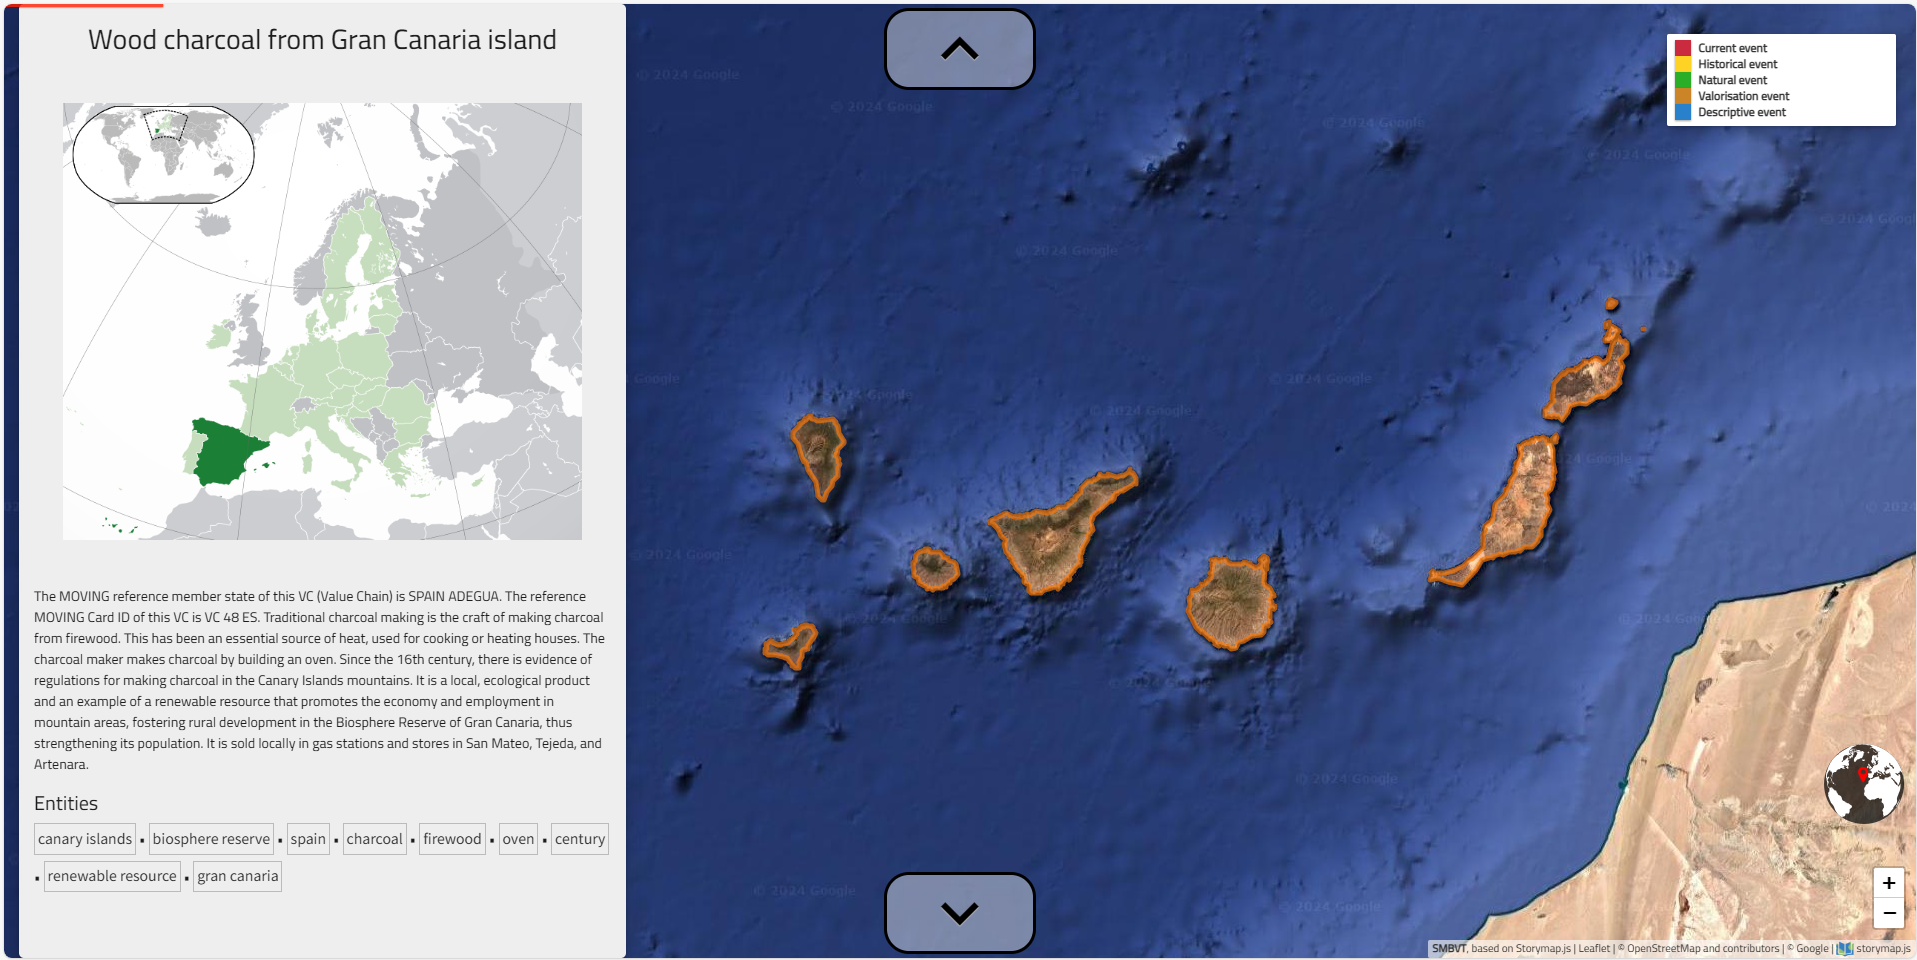
\includegraphics[width=\linewidth]{img/charcoal1.png}
    \caption{Caption here}\label{fig:charcoal1}\par 
    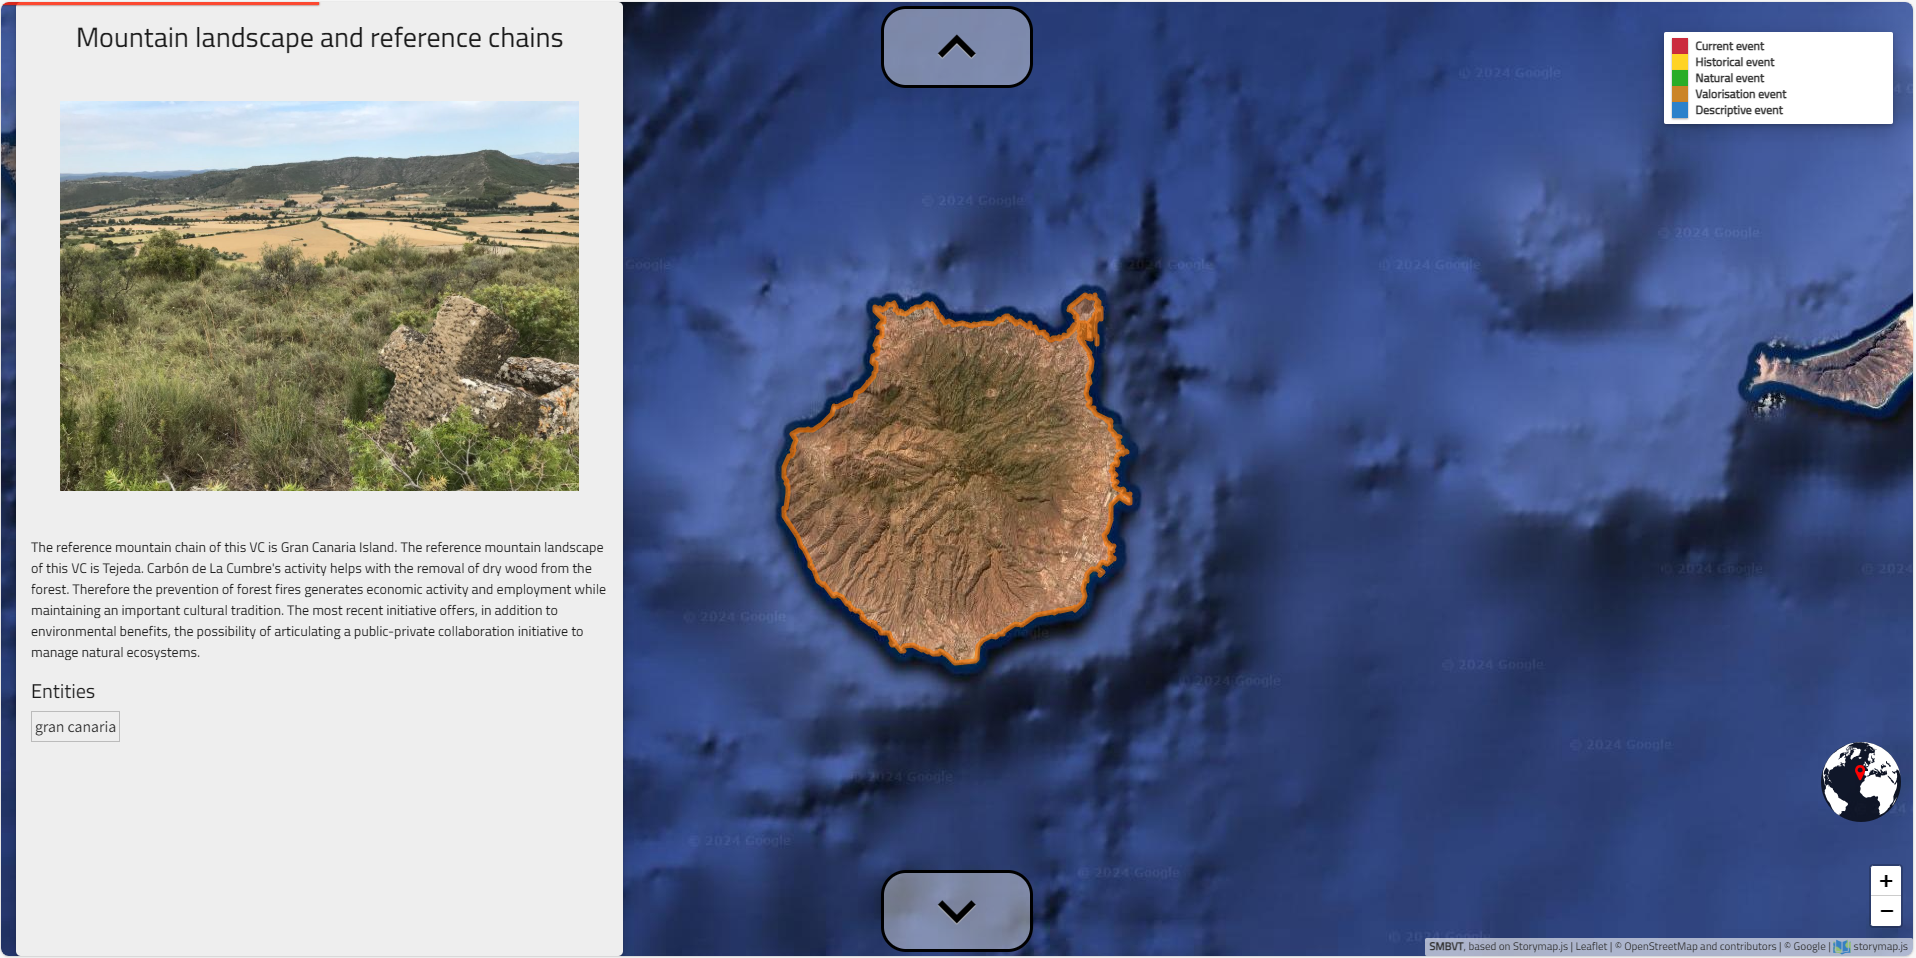
\includegraphics[width=\linewidth]{img/charcoal2.png}
    \caption{Caption here}\label{fig:charcoal2}\par 
\end{multicols}
\begin{multicols}{2}
    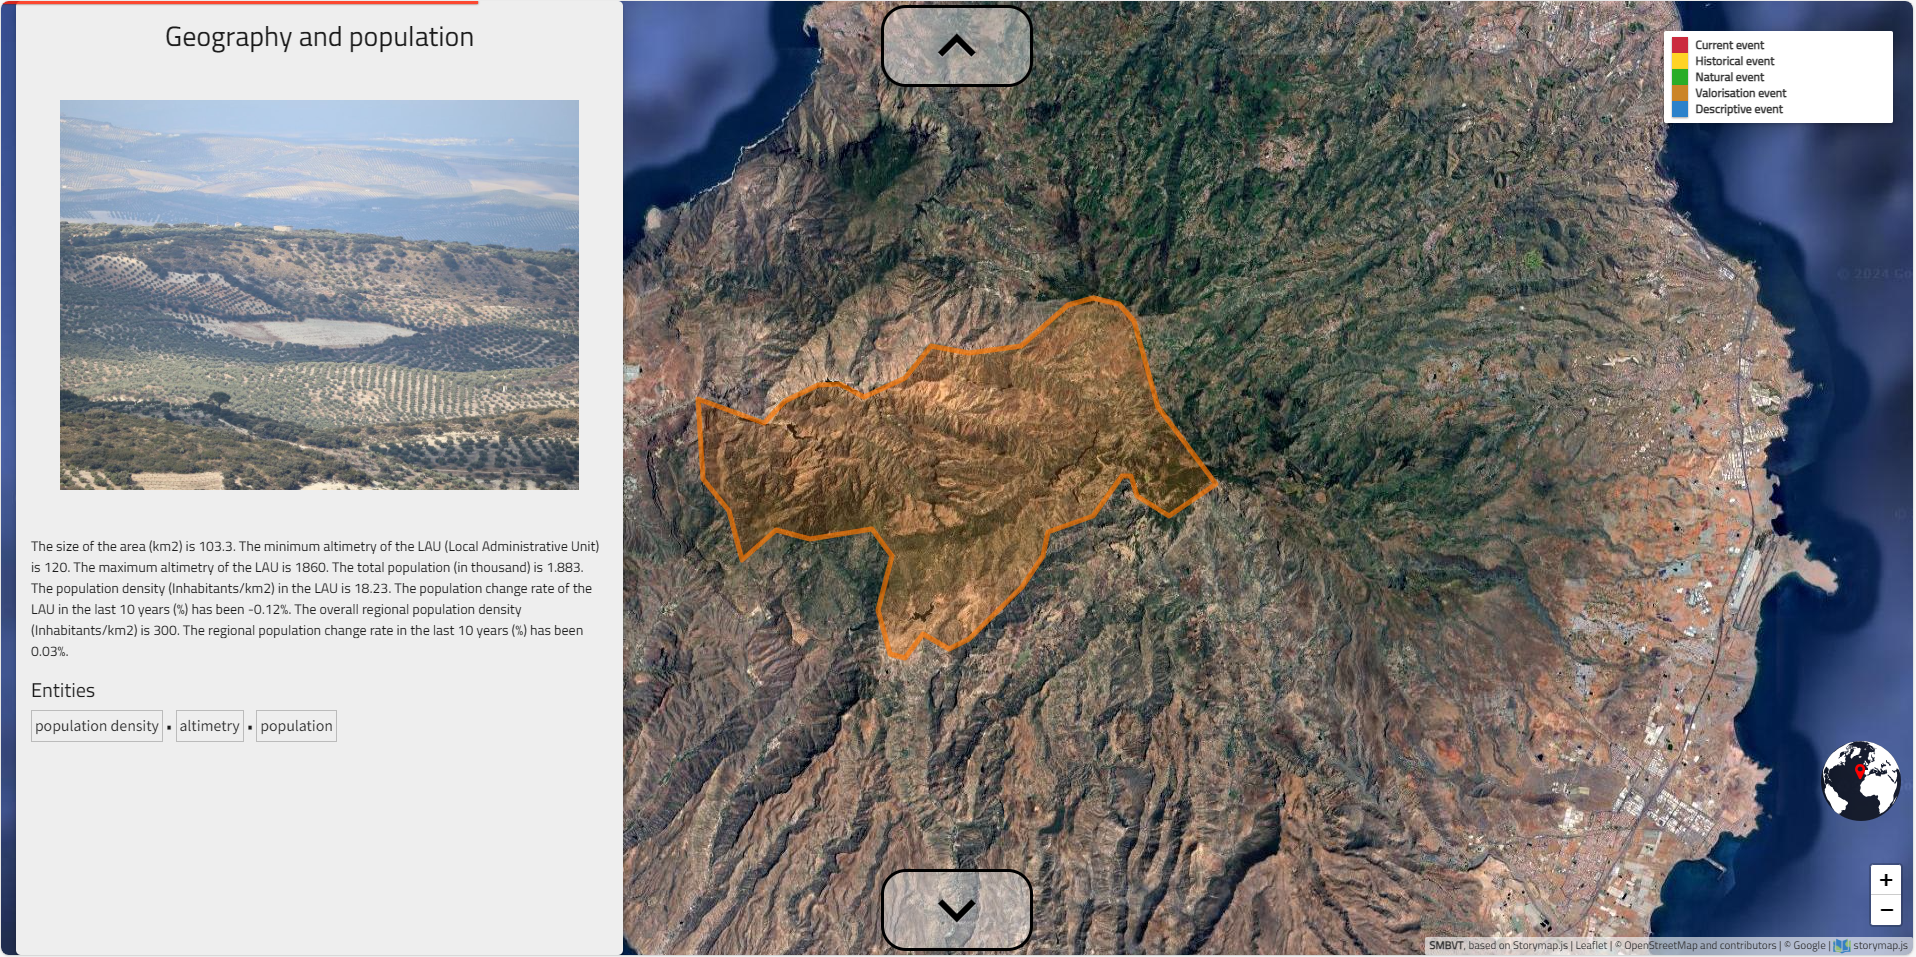
\includegraphics[width=\linewidth]{img/charcoal3.png}
    \caption{Caption here}\label{fig:charcoal3}\par
    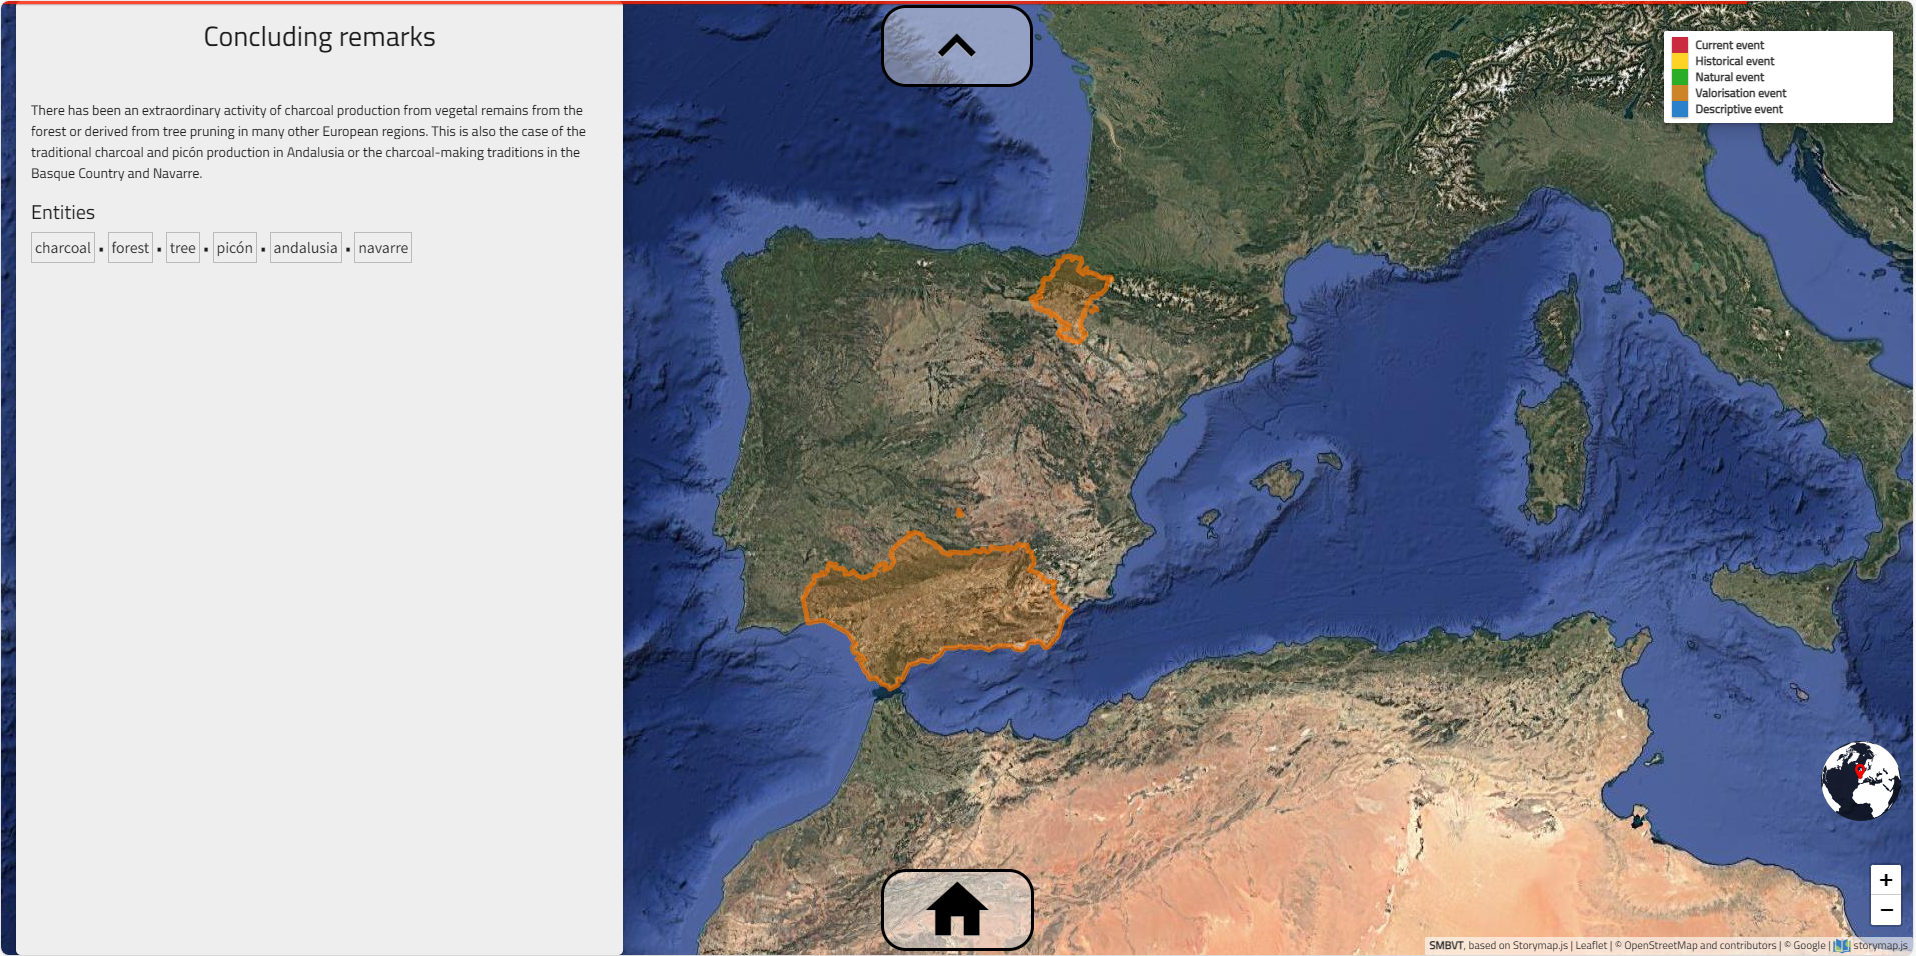
\includegraphics[width=\linewidth]{img/charcoal4.png}
    \caption{Caption here}\label{fig:charcoal4}\par
\end{multicols}
\end{figure*}

\subsubsection{Components of SMBVT Story Maps}
In SMBVT, a story map comprises several interactive components that guide the user through the narrative in a plot-defined sequence. Each story event is represented on the map as a distinct “slide,” containing essential information that enhances the storytelling experience. Each event on the story map is associated with:

\begin{itemize}
    \item \textbf{Geographic Location}: Geographic coordinates or polygons are displayed on the map, providing spatial context (\Cref{fig:charcoal1,fig:charcoal2,fig:charcoal3,fig:charcoal4}).
    \item \textbf{Media Objects}: An image or video linked to each event, known as the "media object", serves as a preview and provides visual engagement (\Cref{fig:charcoal1,fig:charcoal2,fig:charcoal3}).
    \item \textbf{Descriptive Text}: A title and narrative description enrich each event’s context (\Cref{fig:charcoal1,fig:charcoal2,fig:charcoal3,fig:charcoal4}).
    \item \textbf{Entities}: Links to external sources, including Wikidata entities and digital objects on platforms like Europeana, facilitate deeper exploration (\Cref{fig:charcoal1,fig:charcoal2,fig:charcoal3,fig:charcoal4}).
\end{itemize}

There are two arrows, one at the center top of the page and the other at the bottom, allowing navigation through the slides. The last slide (\Cref{fig:charcoal4}) has a home icon to return to the first slide.

Each slide on the story map is divided into two parts:
\begin{itemize}
    \item \textbf{Background Map}: Displayed on the right side, the background map shows the geographical elements.
    \item \textbf{Event Information}: Displayed on the left side, this section provides detailed information about each event, including media objects and descriptive text.
\end{itemize}

Storymap.js was selected for its flexibility in handling large background maps and supporting data represented as JSON. Its slide-based approach to storytelling aligns well with SMBVT’s narrative structure, where each event is encapsulated in a slide that combines spatial and informational elements.

\begin{figure}[h!tb]
    \centerline {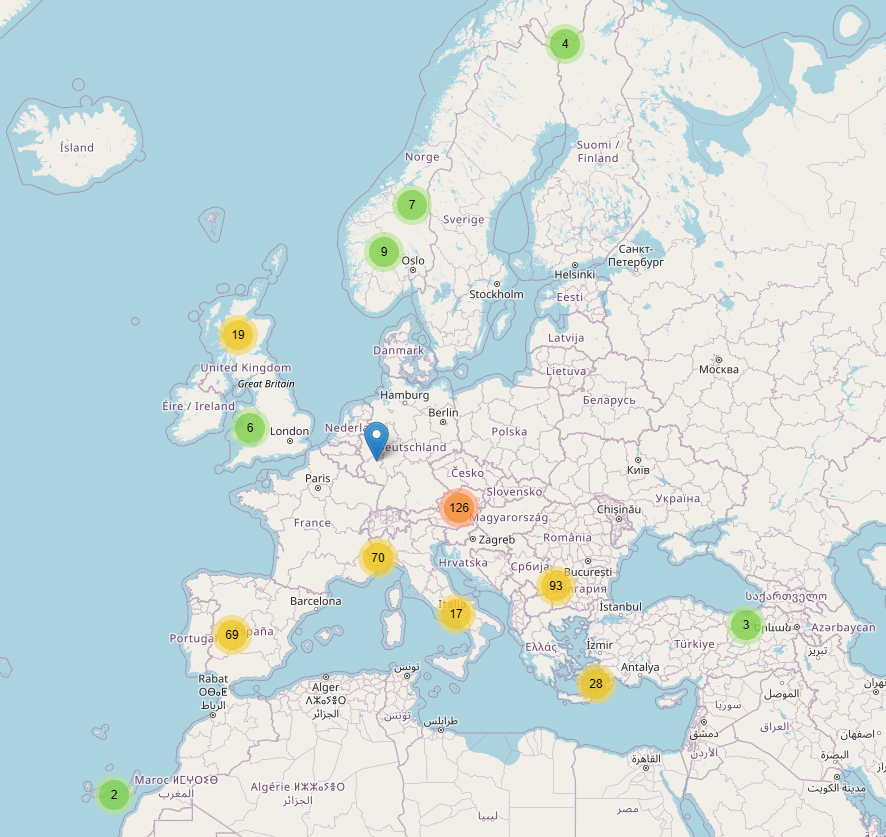
\includegraphics[scale=0.6]{img/allStorymapsMoving.png}}
    \caption{All 454 Story Maps on the map}
    \label{fig:allStorymaps}
\end{figure}

All story maps can be accessed through a map interface that allows users to explore an additional geospatial dimension, connecting each story with others in spatial relation (\Cref{fig:allStorymaps}).

\subsubsection{Publication and Static Web Application Generation}
Once a story map is fully compiled, SMBVT generates a static Web application. This Web app encapsulates all necessary JSON data, JavaScript functionality, and external libraries, creating an interactive experience for end users. The final output enables users to explore the narrative through a series of map-based events, fully contained within a single Web application.

SMBVT’s story maps, facilitated by the customization of StoryMapJS, offer a dynamic and immersive way to present narratives within a spatial context. This tool’s flexibility and ease of integration make it highly effective for storytelling in digital and educational applications, connecting users with content interactively and meaningfully.


\section{Medioeval and Reinassence Geographic Literature (IMAGO Project 2020-2024)}\label{VII-sec:imago}

The \acrfull{IMAGOLabel} project \cite{IMAGOProject} is dedicated to the study of medieval and Renaissance geographical works, ranging from the 6th to the 15th centuries. This interdisciplinary project aims to provide a comprehensive survey of geographic works, classifying authors, genres, and contents, while also collecting manuscripts, editions, and bibliographies of these works. 

\acrshort{IMAGOLabel} focuses on building a web portal and a knowledge base (KB) to facilitate research in medieval geography by using Semantic Web technologies. 

For the \acrshort{IMAGOLabel} project, the dataset focused on geospatial data found in historical texts, particularly locations cited in medieval manuscripts. The second module of the algorithm was instrumental in enriching this dataset, as it incorporated geospatial information from \acrshort{OSMLabel} and linked these places to relevant Wikidata entities.

Using the NOnt+S ontology framework, I developed a knowledge base to represent geospatial knowledge within historical geographic texts. The application of semantic reasoning to this dataset revealed connections between geographic references across various historical texts, providing new insights into medieval geography. The ontology was also used to model the structure of medieval travel narratives, preserving the historical context of these journeys. This approach facilitated the analysis and comparison of different medieval travel routes, cultural exchanges, and traveler experiences, enhancing our understanding of historical travel patterns.

\subsection{Linking and Geospatial Enrichment}\label{VII-subsec:imago-linking}

In the annotation of medieval and Renaissance geographical texts, scholars employed a semi-automatic tool designed to capture and document extensive bibliographic details. These details encompassed not only the geographical texts themselves but also the manuscripts and printed editions through which these texts have been transmitted. Given the inherently geographical nature of these works, the annotations were enriched with a comprehensive set of geospatial data. This data spanned a wide range of entities, including the geographic locations mentioned within the texts, as well as the present-day locations of the libraries and archives that held these manuscripts and print editions.

The geospatial information collected from these texts was significantly enhanced by linking it to a variety of geospatial knowledge bases. The historical dimension of these works posed a unique challenge: many of the geographical places referenced either no longer exist or have undergone substantial transformation across the centuries. Addressing this challenge required linking the annotated geospatial data not only to contemporary databases but also to specialized historical knowledge repositories. One such critical resource was Pleiades \cite{simonPleiadesGazetteerPelagios2016}, a robust and authoritative knowledge base dedicated to ancient geographic locations. The integration with Pleiades enabled scholars to situate historical places accurately within their appropriate temporal and cultural contexts, facilitating a more nuanced understanding of these geographic references. This phase of linking was, therefore, pivotal in establishing a reliable and contextually aware framework for the spatial data embedded within the medieval and Renaissance texts.

The \acrshort{IMAGOLabel} knowledge base, structured using the same foundational ontologies as the NOnt framework, the CRM and the LRMoo, facilitates seamless interoperability between these two knowledge systems. This common ontological foundation permits the merging of both knowledge bases, ensuring that data exchange and integration processes are both efficient and semantically coherent. The structural compatibility between \acrshort{IMAGOLabel} and NOnt+S thus allows for enhanced information retrieval and more sophisticated knowledge representation.

Subsequent to the linking phase, a comprehensive geospatial enrichment phase was undertaken. This phase utilized the \Cref{alg:entityextraction}, a module explicitly developed to support advanced querying of linked data sources. Through the execution of these queries, the scholars were able to extract additional geospatial details from widely used and openly accessible datasets such as \acrshort{OSMLabel} and Wikidata. These datasets offered a rich repository of information, including precise coordinates and polygonal representations of various geographical features. By incorporating this enriched data, the scholars were able to augment the initial annotations, providing a more detailed and accurate spatial representation of the places referenced in the texts.

This enrichment process not only increased the depth of the annotated geospatial data but also enabled the visualization and mapping of historical locations described in the medieval and Renaissance texts. Such visualizations afford new insights into the spatial dynamics of the works, illuminating the complex geographical relationships that shaped the understanding of space and place in these historical periods. Consequently, the enriched geospatial framework contributes to a more profound and comprehensive exploration of the historical and cultural landscapes depicted in these texts.


\subsection{Knowledge Graph Creation and Storage}\label{VII-subsec:imago-kg}

The \acrshort{IMAGOLabel} knowledge graph\footnote{The graph can be downloaded at \url{https://geosparql.isti.cnr.it/ontology/imago.owl}} was constructed in accordance with the comprehensive framework outlined in  \Cref{chap:SW-framework}. This framework provided a systematic approach, ensuring that each stage of knowledge graph development adhered to the principles of semantic web technologies, data interoperability, and ontological consistency. The creation process involved a design phase, wherein concepts and relationships relevant to the domain of medieval and Renaissance geographical works were modeled using well-established ontologies, particularly the CIDOC Conceptual Reference Model (CRM) and the Library Reference Model object-oriented version (LRMoo). These ontologies served as the foundational schema, ensuring semantic clarity and facilitating seamless integration with other linked datasets.

A key consideration during the development of the \acrshort{IMAGOLabel} knowledge graph was the need to accommodate the rich geospatial information inherent in the annotated works. To this end, the graph was structured to support complex geospatial queries, a requirement that was addressed through the integration of GeoSPARQL. GeoSPARQL, an extension of the SPARQL query language specifically designed for geospatial data, provided the necessary tools to handle the intricate spatial relationships and geometries associated with the geographical references in the texts. By leveraging GeoSPARQL, the knowledge graph not only enabled efficient querying of spatial data but also supported advanced geospatial operations, such as the retrieval of location-based information and the computation of spatial relationships.

The storage of the \acrshort{IMAGOLabel} knowledge graph was implemented using a Fuseki triplestore, a robust and scalable RDF (Resource Description Framework) database solution optimized for handling linked data. Fuseki’s compatibility with GeoSPARQL allowed for the seamless storage and retrieval of geospatial data, ensuring that the knowledge graph remained performant and responsive to complex queries. Furthermore, the use of a triplestore architecture ensured that the data remained flexible and easily extendable, accommodating future updates and integrations with minimal disruption.

By employing these technologies, the \acrshort{IMAGOLabel} knowledge graph became a powerful tool for exploring and analyzing the intricate web of relationships between historical texts, places, and cultural heritage objects. The combination of semantic precision, geospatial enrichment, and efficient data storage ensured that the graph could be used effectively by scholars and researchers to gain new insights into the spatial and temporal dimensions of medieval and Renaissance geography. Thus, the creation and storage strategy of the \acrshort{IMAGOLabel} knowledge graph exemplified a sophisticated approach to knowledge representation, grounded in the principles of the semantic web and designed to support both scholarly inquiry and digital heritage preservation.


\subsection{Consistency of the Knowledge Graph}\label{VII-subsec:imago-consistency}

To check the consistency of the knowledge graph is employed Openllet\cite{galigatorGaligatorOpenllet2024} as described in the \Cref{chap:SW-framework}. These tools analyze the graph for logical inconsistencies, such as contradictory relationships or incorrect classifications. For instance, if a geographic work is incorrectly linked to a location that did not exist during the time period in question, the reasoning engine can flag this as an inconsistency.

Another important aspect of maintaining consistency is ensuring the proper integration of external data sources. Linked Data often involves incorporating information from various knowledge bases, each of which may use slightly different ontological models. Alignment of these models through ontology matching and mapping techniques ensures that the data remains semantically coherent across sources.

Regular consistency checks are also necessary as the knowledge graph evolves. As new data is added or existing data is updated, automatic or semi-automatic validation mechanisms must be in place to ensure that the graph remains logically sound and free from errors.

\subsection{Requirement Analysis and Querying}\label{VII-subsec:imago-querying}

Before effective querying of the knowledge graph can take place, a thorough requirement analysis must be conducted. This involves identifying the key research questions that the knowledge graph is intended to address, as well as the specific types of information that users will need to retrieve. Requirement analysis serves as the foundation for designing efficient GeoSPARQL queries and ensuring that the structure of the knowledge graph supports the desired use cases.

During the requirement analysis phase, scholars and domain experts collaborate to outline the types of queries they anticipate running against the knowledge graph. These could include retrieving all works that reference a particular geographic location, finding all manuscripts stored in a specific archive, or identifying the spatial relationships between different historical places. The specific needs of the user community must be thoroughly understood so that the data model, ontologies, and graph structure are optimized for these queries.

Once the requirements are clearly defined, the next step is to create GeoSPARQL queries that can extract the relevant data. GeoSPARQL is a powerful query language specifically designed for querying \acrshort{RDFLabel} datasets. Its pattern-matching capabilities enable users to express complex queries involving multiple entities and relationships. For instance, a query could retrieve all places mentioned in a set of geographical works, along with their modern equivalents retrieved from external geospatial knowledge bases such as \acrshort{OSMLabel}.

Query optimization is another important consideration during this phase. As knowledge graphs grow in size and complexity, performance can become an issue. Therefore, the design of \acrshort{SPARQLLabel} queries must account for factors such as execution time, memory usage, and indexing. Efficient query design ensures that the knowledge graph remains responsive and usable, even as the amount of data increases. Additionally, designing and executing a distinct set of queries in this domain, separate from those outlined in Section \ref{VII-subsec:moving-querying}, is essential to reinforce the robustness of responses to Research Question 2 (\ref{quote:rq2}). This approach not only validates the applicability of the methodology across diverse contexts but also underscores the adaptability and scalability of the proposed query framework.


We focussed on four types of knowledge-extraction targets, corresponding to four GeoSPARQL queries regarding different and complementary aspects of medieval manuscripts and their related place cited:
\begin{enumerate}
    \item The works that mention places located in France (Q5)
    \item The places located within a 0.2-degree buffer around the Via Francigena (Q6)
    \item The places in Italy that are mentioned in works contained in manuscripts written in the fifteenth century (Q7)
    \item The authors who have visited the Holy Land (Q8)
\end{enumerate}

The information extracted by these queries covered the interests of the \acrshort{IMAGOLabel} scholars. It would have been hard, indeed, to extract the same information through the usual data representation and technology adopted by this community. Based on the query results\footnote{The visualization of the queries can be replicated via the web application accessible at \url{https://github.com/prate91/GeoSPARQL-queries-visualization-for-thesis}}, we calculated the same standard performance of \Cref{VII-subsec:moving-querying}. 

Even for \acrshort{IMAGOLabel} queries, the performance metrics displayed in \Cref{tab:evaluationQueries} uniformly indicate a perfect score of 1 for Precision, Recall, and F1. This consistency across diverse queries further corroborates the comprehensive reliability and robustness of our knowledge graph. The ability to maintain such high performance across various query scenarios reflects the effectiveness of the semantic structures and inference mechanisms we have implemented. These results underscore the high fidelity and precision of our data representation, which facilitates accurate and exhaustive retrieval, thereby enhancing the utility and reliability of our system. In the following, we report the details of the queries and the corresponding results.

\begin{table}[H]
    \centering
        \caption{Precision, Recall, and F1 measurements of IMAGO queries.}
    \label{tab:evaluationQueriesIMAGO}
    \begin{tabular}{|l|l|l|l|}
    \hline
 Query & Precision & Recall & F1\\
\hline
        Q5 & 1 & 1 & 1\\ \hline
        Q6 & 1 & 1 & 1\\ \hline
        Q7 & 1 & 1 & 1 \\  \hline
        Q8 & 1 & 1 & 1 \\ \hline
    \end{tabular}
\end{table}

\subsubsection*{Q5 - The works that mention places located in France}
In the following, we report the GeoSPARQL query corresponding to Q5. The results are displayed in \Cref{fig:france}.

\begin{lstlisting}[caption=GeoSPARQL Query 5, label={lst:query5}]
PREFIX /*!\gls{imago}!*/ <https://imagoarchive.it/ontology/>
PREFIX /*!\gls{wd}!*/ <http://www.wikidata.org/entity/>
PREFIX /*!\gls{geo}!*/ <http://www.opengis.net/ont/geosparql#>
PREFIX /*!\gls{ecrm}!*/ <http://erlangen-crm.org/200717/>
PREFIX /*!\gls{ilrm}!*/ <http://imagoarchive.it/ilrmoo/>
PREFIX /*!\gls{osm}!*/ <https://www.openstreetmap.org/>
PREFIX /*!\gls{osm2rdfkey}!*/ <https://osm2rdf.cs.uni-freiburg.de/rdf/key#>
PREFIX /*!\gls{geof}!*/ <http://www.opengis.net/def/function/geosparql/> 

SELECT DISTINCT ?title ?authorName ?toponymName ?wktPlace
  FROM <https://geosparql.isti.cnr.it/fuseki/imago/archive>
WHERE {
  ?exp_cre a ilrm:F28_Expression_Creation ;
  	         ilrm:R17_created ?work ;
  	         ecrm:P14_carried_out_by ?author .	
  ?author a imago:Author ;
          ecrm:P1_is_identified_by/ecrm:P190_has_symbolic_content ?authorName .
  ?work a ilrm:F2_Expression ;
        ecrm:P102_has_title/ecrm:P190_has_symbolic_content ?title ;
        ecrm:P106_is_composed_of ?toponym .
  ?place imago:is_identified_by_toponym ?toponym ;
         geo:asWKT ?wktPlace .
  ?toponym ecrm:P190_has_symbolic_content ?toponymName .

  { 
    SELECT ?wktFrance 
    WHERE {
        SERVICE <https://qlever.cs.uni-freiburg.de/api/osm-planet> { 
            ?osm_id osm2rdfkey:wikidata wd:Q142 ;
                    a osm:relation ;
                    geo:hasGeometry ?geometryFrance .
            ?geometryFrance geo:asWKT ?wktFrance .     
        } 
    } LIMIT 1
  }
  FILTER(geof:sfWithin(?wktPlace,?wktFrance)). 
} 
\end{lstlisting}

% The query retrieves the work titles and authors along with the toponyms the works mention. The WHERE clause contains the conditions that need to be satisfied for each result. It involves several semantic-triple patterns connected by the "." or ";" operators. In this clause, we retrieve the work titles, authors, toponyms, and the polygons of the places identified by the toponyms. A nested SELECT statement allows retrieving the WKT geometry of France (Q142) from the QLever \acrshort{SPARQLLabel} server of the University of Freiburg. Finally, the FILTER clause selects the places included within the France polygon.


The \Cref{lst:query5} is designed to retrieve distinct titles of works, author names, place names (toponyms), and the \acrshort{WKTLabel} representation of place geometries within France. The purpose of this query is to locate specific works within the \acrshort{IMAGOLabel} archive, ensuring that the places mentioned are geographically located within the boundaries of France. The query performs a spatial relationship check to filter only those places that fall within France’s geographical borders.

The query starts by defining various prefixes (lines 1-8) that are essential for interpreting and utilizing the data from different ontologies. 

The \texttt{SELECT DISTINCT} statement (line 10) specifies the output variables:
\begin{itemize}
    \item \texttt{?title} - Title of the work.
    \item \texttt{?authorName} - Name of the author of the work.
    \item \texttt{?toponymName} - Name of the place (toponym).
    \item \texttt{?wktPlace} - \acrshort{WKTLabel}representation of the place's geometry.
\end{itemize}

The \texttt{FROM} clause (line 11) indicates the source graph:\\
\texttt{https://geosparql.isti.cnr.it/fuseki/imago/archive}.

The main \texttt{WHERE} block (lines 12-27) contains the conditions that define the data to be retrieved. It is divided into several graph patterns:

\textbf{Graph Patterns for Expression Creation and Author}
\begin{itemize}
    \item The triple pattern at line 13, \texttt{?exp\_cre a \gls{ilrm}F28\_Expression\_Creation}, identifies instances of expression creation events.
    \item The pattern \texttt{\gls{ilrm}R17\_created ?work} links these events to the created works.
    \item The triple pattern \texttt{\gls{ecrm}P14\_carried\_out\_by ?author} identifies the author responsible for the creation.
\end{itemize}

\textbf{Graph Patterns for Author Details}
\begin{itemize}
    \item \texttt{?author a imago:Author} ensures that the \texttt{?author} variable is of the type \textit{Author}.
    \item The \texttt{\gls{ecrm}P1\_is\_identified\_by/\gls{ecrm}P190\_has\_symbolic\_content ?authorName} pattern retrieves the author’s name.
\end{itemize}

\textbf{Graph Patterns for Work and Title}
\begin{itemize}
    \item \texttt{?work a \gls{ilrm}F2\_Expression} identifies works as instances of the \\ \texttt{F2\_Expression} class.
    \item \texttt{\gls{ecrm}P102\_has\_title/\gls{ecrm}P190\_has\_symbolic\_content ?title} retrieves the title of each work.
    \item \texttt{\gls{ecrm}P106\_is\_composed\_of ?toponym} links the work to toponyms (place names) associated with it.
\end{itemize}

\textbf{Graph Patterns for Place Geometry}
\begin{itemize}
    \item \texttt{?place \gls{imago}is\_identified\_by\_toponym ?toponym} connects a place with its toponym.
    \item \texttt{\gls{geo}asWKT ?wktPlace} retrieves the \acrshort{WKTLabel} geometry of the place.
    \item \texttt{?toponym \gls{ecrm}P190\_has\_symbolic\_content ?toponymName} retrieves the symbolic content (name) of the toponym.
\end{itemize}

\textbf{Nested SELECT Clause}
A nested \texttt{SELECT} block (lines 20-27) retrieves the \acrshort{WKTLabel} geometry of France. The details are as follows:
\begin{itemize}
    \item \textbf{SERVICE Clause}: The \texttt{SERVICE} keyword (line 22) is used to access the external QLever endpoint \url{https://qlever.cs.uni-freiburg.de/api/osm-planet}.
    \item The triple pattern \texttt{?osm\_id \gls{osm2rdfkey}wikidata \gls{wd}Q142} (line 23) retrieves the \acrshort{OSMLabel} relation that corresponds to the Wikidata entity for France (\gls{wd}Q142).
    \item \texttt{geo:hasGeometry ?geometryFrance} retrieves the geometry of France.
    \item \texttt{geo:asWKT ?wktFrance} provides the \acrshort{WKTLabel} representation of this geometry.
    \item The \texttt{LIMIT 1} clause restricts the results to a single instance.
\end{itemize}

\textbf{Spatial Filter}
The \texttt{FILTER} clause (line 28) uses the \texttt{\gls{geof}sfWithin} function to check if the place geometry (\texttt{?wktPlace}) is spatially within the geometry of France (\texttt{?wktFrance}). This ensures that only places within France are considered in the results.

\begin{figure}[h!tb]
    \centerline {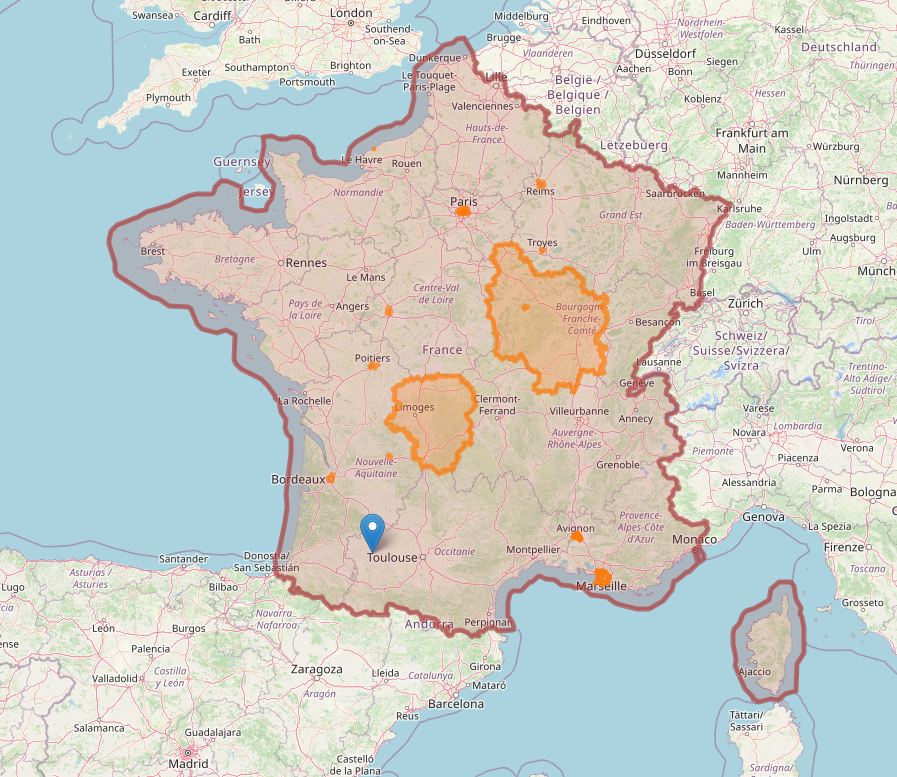
\includegraphics[scale=0.6]{img/france.png}}
    \caption{Visualization of Q5}
    \label{fig:france}
\end{figure}


\subsubsection*{Q6 - The places located within a 0.2-degree buffer around the Via Francigena}
In the following, we report the GeoSPARQL query corresponding to Q6\footnote{the polygon of via francigena is abbreviated for presentation purposes, it is accessible at \url{https://l.cnr.it/6eyzp}}. The results are displayed in \Cref{fig:francigena}.

\begin{lstlisting}[caption=GeoSPARQL Query 6, label={lst:query6}]
PREFIX /*!\gls{imago}!*/ <https://imagoarchive.it/ontology/>
PREFIX /*!\gls{xsd}!*/ <http://www.w3.org/2001/XMLSchema#>
PREFIX /*!\gls{ecrm}!*/ <http://erlangen-crm.org/200717/>
PREFIX /*!\gls{ilrm}!*/ <http://imagoarchive.it/ilrmoo/>
PREFIX /*!\gls{igen}!*/ <https://imagoarchive.it/thes/tid/>
PREFIX /*!\gls{uom}!*/ <http://www.opengis.net/def/uom/OGC/1.0/>
PREFIX /*!\gls{geo}!*/ <http://www.opengis.net/ont/geosparql#>
PREFIX /*!\gls{geof}!*/ <http://www.opengis.net/def/function/geosparql/> 

SELECT DISTINCT ?title ?authorName ?wktPlace ?francigena
FROM <https://geosparql.isti.cnr.it/fuseki/imago/archive>
WHERE { 
  BIND("LINESTRING(1.11419 51.26638 0, ... ,12.46387 41.90754 0)"^^geo:wktLiteral AS ?francigena)
  ?exp_cre a ilrm:F28_Expression_Creation ;
  		     ilrm:R17_created ?work ;
  		     ecrm:P14_carried_out_by ?author .	
  ?author a imago:Author ;
          ecrm:P1_is_identified_by/ecrm:P190_has_symbolic_content ?authorName .
  ?work a ilrm:F2_Expression ;
        ecrm:P102_has_title/ecrm:P190_has_symbolic_content ?title ;
  		  ecrm:P106_is_composed_of ?toponym .
  ?place imago:is_identified_by_toponym ?toponym ;
         geo:asWKT ?wktPlace .
  ?toponym ecrm:P190_has_symbolic_content ?toponymName .
  ?work imago:has_genre igen:100021 . # itineraria
 FILTER(geof:sfWithin(
        ?wktPlace,
        geof:buffer(?francigena, 0.2, uom:degree))). }
\end{lstlisting}

% The query retrieves the work titles and authors along with the toponyms the works mention. In the WHERE clause, we retrieve the work titles and authors and the toponyms as well as the polygons of the places identified by the toponyms. Furthermore, we set the value of the work literary genre equal to itineraria. Indeed, we think that a study on the knowledge of places located near the via Francigena is more significant if conducted on works belong to the genres of travel literature. The Via Francigena is an ancient road and pilgrimage route running from Canterbury in England, through France and Switzerland, to Rome and then to Apulia, Italy, where there were ports of embarkation for the Holy Land. Itineraria genre has a unique identifier (100021) that came from a literary genres thesaurus built by the IMAGO scholars based on the subject indexing tool Nuovo Soggettario.
% Finally, the FILTER clause selects the places that are included within a buffer of 0.2 degrees created around the Francigena polygon, specified in the BIND operator.


The \Cref{lst:query6} retrieves distinct titles of works, author names, place geometries, and the geometry of the Via Francigena, filtered to ensure that the places are located within a 0.2-degree buffer zone of the Via Francigena. The Via Francigena is represented as a LINESTRING in \acrshort{WKTLabel} format.

Similar to query 5, there is a definition of prefixes and the \texttt{FROM} clause.

The \texttt{SELECT DISTINCT} statement (line 10) specifies:
\begin{itemize}
    \item \textit{title} - Title of the work.
    \item \textit{authorName} - Name of the author.
    \item \textit{wktPlace} - \acrshort{WKTLabel} representation of the place geometry.
    \item \textit{francigena} - Geometry of the Via Francigena in \acrshort{WKTLabel} format.
\end{itemize}

\textbf{WHERE Clause}
The main \texttt{WHERE} block (lines 12-26) defines the data retrieval conditions:
\begin{itemize}
    \item \texttt{BIND} statement binds a LINESTRING \acrshort{WKTLabel} representation of the Via Francigena to the variable \texttt{?francigena}.
    \item Patterns at lines 13-15 link expression creation events, works, and authors.
    \item Author details are retrieved using  \\ \texttt{ecrm:P1\_is\_identified\_by/ecrm:P190\_has\_symbolic\_content ?authorName}.
    \item Work details are retrieved, including title and toponyms.
    \item Place geometries are linked and retrieved in \acrshort{WKTLabel} format.
    \item The work must belong to the \texttt{itineraria} genre, specified by \texttt{igen:100021}.
\end{itemize}

\textbf{Spatial Filter}
The \texttt{FILTER} clause (line 26) uses \texttt{geof:sfWithin} to ensure that the places are within a 0.2-degree buffer zone of the Via Francigena.

\begin{figure}[h!tb]
    \centerline {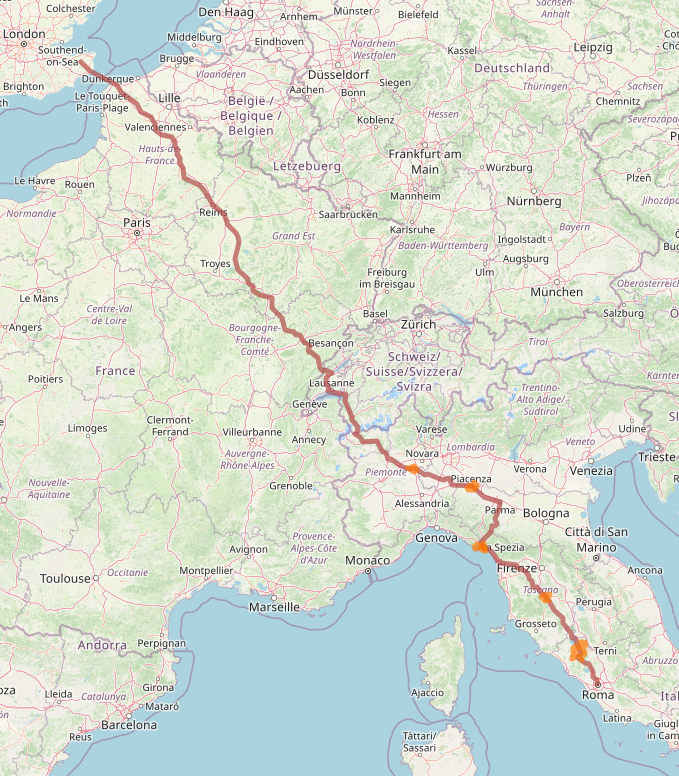
\includegraphics[scale=0.6]{img/francigena.png}}
    \caption{Visualization of Q6}
    \label{fig:francigena}
\end{figure}

\subsubsection*{Q7 - The places in Italy that are mentioned in works contained in manuscripts written in the fifteenth century }
In the following, we report the GeoSPARQL query corresponding to Q7. The results are displayed in \Cref{fig:italy}.

\begin{lstlisting}[caption=GeoSPARQL Query 7, label={lst:query7}]
PREFIX /*!\gls{xsd}!*/ <http://www.w3.org/2001/XMLSchema#>
PREFIX /*!\gls{rdf}!*/ <http://www.w3.org/1999/02/22-rdf-syntax-ns#>
PREFIX /*!\gls{rdfs}!*/ <http://www.w3.org/2000/01/rdf-schema#>
PREFIX /*!\gls{ecrm}!*/ <http://erlangen-crm.org/200717/>
PREFIX /*!\gls{ilrm}!*/ <http://imagoarchive.it/ilrmoo/>
PREFIX /*!\gls{imago}!*/ <https://imagoarchive.it/ontology/>
PREFIX /*!\gls{geo}!*/ <http://www.opengis.net/ont/geosparql#>
PREFIX /*!\gls{osm}!*/ <https://www.openstreetmap.org/>
PREFIX /*!\gls{osm2rdfkey}!*/ <https://osm2rdf.cs.uni-freiburg.de/rdf/key#>
PREFIX /*!\gls{geof}!*/ <http://www.opengis.net/def/function/geosparql/> 
PREFIX /*!\gls{wd}!*/ <http://www.wikidata.org/entity/>
SELECT DISTINCT ?authorName ?title ?toponymName ?wktPlace 
	FROM <https://geosparql.isti.cnr.it/fuseki/imago/archive>
		WHERE {
    ?exp_cre a ilrm:F28_Expression_Creation ;
  		     ilrm:R17_created ?work ;
         ecrm:P14_carried_out_by ?author ;
      		 ilrm:R18_created ?manuscript .
  ?author a imago:Author ;
          ecrm:P1_is_identified_by/ecrm:P190_has_symbolic_content ?authorName .
  ?work a ilrm:F2_Expression ;
        ecrm:P102_has_title/ecrm:P190_has_symbolic_content ?title ;
        ecrm:P106_is_composed_of ?toponym . 
  		?place imago:is_identified_by_toponym ?toponym ;
         		geo:asWKT ?wktPlace .
  		?toponym ecrm:P190_has_symbolic_content ?toponymName .
		?manifestation ilrm:R7i_is_materialized_in ?manuscript .
   		?manuscript ecrm:P1_is_identified_by/ecrm:P190_has_symbolic_content ?signature ;
		              ecrm:P50_has_current_keeper ?library ;
		              ecrm:P46_is_composed_of/ecrm:P1_is_identified_by/ecrm:P190_has_symbolic_content ?folios .
  		?library ecrm:P74_has_current_or_former_residence ?libraryPlace ;
		  			ecrm:P1_is_identified_by/ecrm:P190_has_symbolic_content ?libraryName .
  		?libraryPlace imago:is_identified_by_toponym ?top .
            ?top ecrm:P190_has_symbolic_content ?libraryPlaceName .
	  	?manifestation_creation ilrm:R24_created  ?manifestation ;
	 		        ecrm:P4_has_time-span/ecrm:P170i_time_is_defined_by ?date_manuscript ;
	    				:has_start_date ?start_date_manuscript ;
	 				:has_end_date ?end_date_manuscript .
		    FILTER("1401-01-01T00:00:00Z"^^xsd:dateTime <= ?start_date_manuscript && ?start_date_manuscript <= "1500-01-01T00:00:00Z"^^xsd:dateTime)
            FILTER("1401-01-01T00:00:00Z"^^xsd:dateTime <= ?end_date_manuscript && ?end_date_manuscript <= "1500-01-01T00:00:00Z"^^xsd:dateTime)
  BIND(CONCAT(?libraryPlaceName, ", ", ?libraryName, ", ",?signature, ", ", ?folios) AS ?manuscriptString)
  
  { 
    SELECT ?wktItaly 
    WHERE {
        SERVICE <https://qlever.cs.uni-freiburg.de/api/osm-planet> { 
            ?osm_id osm2rdfkey:wikidata wd:Q38 ;
                    a osm:relation ;
                    geo:hasGeometry ?geometryItaly .
            ?geometryItaly geo:asWKT ?wktItaly .     
        } 
    } LIMIT 1
  }
  FILTER(geof:sfWithin(?wktPlace,?wktItaly)). 
} 
\end{lstlisting}

% The query retrieves the toponyms and the corresponding works and authors in which these places are mentioned. In the WHERE clause, the polygons of the places identified by the toponyms are retrieved. Simultaneously, information regarding manuscripts is retrieved, including the production dates. Subsequently, the time range is established using the FILTER operator. A nested SELECT statement allows retrieving the WKT geometry of Italy (Q38) from the QLever \acrshort{SPARQLLabel} server of the University of Freiburg. Finally, another FILTER clause selects the places included within Italy's polygon.

The \Cref{lst:query7} retrieves distinct author names, work titles, place names, and WKT geometries of places associated with manuscripts created between 1401 and 1500, and stored in libraries within Italy.

Similar to query 5, there is a definition of prefixes and the \texttt{FROM} clause.

The \texttt{SELECT DISTINCT} statement (line 12) specifies:
\begin{itemize}
    \item \textit{authorName} - Author of the work.
    \item \textit{title} - Title of the work.
    \item \textit{toponymName} - Name of the place.
    \item \textit{wktPlace} - WKT representation of the place.
\end{itemize}

\textbf{WHERE Clause}
The \texttt{WHERE} block (lines 13-39) includes:
\begin{itemize}
    \item Patterns linking expression creation events, authors, works, and manuscripts.
    \item Retrieval of author and work details, including titles and toponyms.
    \item Information about manuscripts: signature, library, and folios.
    \item Library details, including residence and name.
    \item Time constraints for manuscript creation (1401-1500) using \texttt{FILTER} clauses.
\end{itemize}

\textbf{Nested SELECT Clause}
A nested \texttt{SELECT} block (lines 33-38) retrieves the WKT geometry of Italy:
\begin{itemize}
    \item Accesses the QLever endpoint to get Italy’s geometry from \acrshort{OSMLabel}.
    \item The \texttt{LIMIT 1} clause restricts to one result for faster retrieval.
\end{itemize}

\subsection*{Spatial Filter}
The \texttt{FILTER} clause (line 39) ensures that places are within Italy’s boundaries using \texttt{geof:sfWithin}.

\begin{figure}[h!tb]
    \centerline {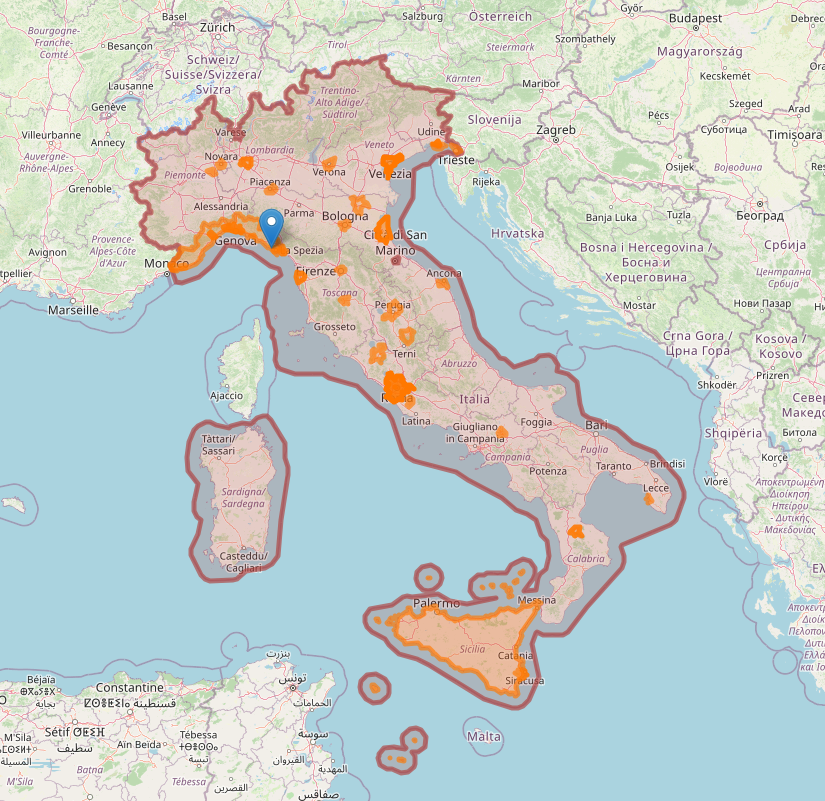
\includegraphics[scale=0.6]{img/italy.png}}
    \caption{Visualization of Q7}
    \label{fig:italy}
\end{figure}

\subsubsection{Q8 - The authors who have visited the Holy Land }
In the following, we report the GeoSPARQL query corresponding to Q8. The results are displayed in \Cref{tab:holyLand}.

\begin{lstlisting}[caption=GeoSPARQL Query 8, label={lst:query8}]
PREFIX /*!\gls{imago}!*/ <https://imagoarchive.it/ontology/>
PREFIX /*!\gls{igen}!*/ <https://imagoarchive.it/thes/tid/>
PREFIX /*!\gls{ecrm}!*/ <http://erlangen-crm.org/200717/>
PREFIX /*!\gls{ilrm}!*/ <http://imagoarchive.it/ilrmoo/>
PREFIX /*!\gls{wdt}!*/ <http://www.wikidata.org/prop/direct/>
PREFIX /*!\gls{wd}!*/ <http://www.wikidata.org/entity/>
PREFIX /*!\gls{geo}!*/ <http://www.opengis.net/ont/geosparql#>
PREFIX /*!\gls{geof}!*/ <http://www.opengis.net/def/function/geosparql/> 
PREFIX /*!\gls{uom}!*/ <http://www.opengis.net/def/uom/OGC/1.0/>

SELECT DISTINCT ?authorName ?title
FROM <https://geosparql.isti.cnr.it/fuseki/imago/archive>
WHERE {
  ?exp_cre a ilrm:F28_Expression_Creation ;
  		     ilrm:R17_created ?work ;
  		     ecrm:P14_carried_out_by ?author .	
  ?author a imago:Author ;
          ecrm:P1_is_identified_by/ecrm:P190_has_symbolic_content ?authorName .
  ?work a ilrm:F2_Expression ;
        ecrm:P102_has_title/ecrm:P190_has_symbolic_content ?title ;
        ecrm:P106_is_composed_of ?toponym . 
  ?place imago:is_identified_by_toponym ?toponym ;
         geo:asWKT ?wktPlace .
  ?toponym ecrm:P190_has_symbolic_content ?toponymName .
  
  ?work imago:has_genre igen:100026 . # Travel journal genre
  igen:100026  imago:has_genre_name ?labelGenre.
  
  { 
    SELECT ?coord 
    WHERE {
      SERVICE <https://query.wikidata.org/bigdata/namespace/wdq/sparql> { 
            wd:Q48175 wdt:P625 ?coord.    
      } 
    } LIMIT 1
  }
  FILTER(geof:sfIntersects(?wktPlace,geof:buffer(?coord,0.3, uom:degree))). 
}  
}  
\end{lstlisting}

% The query retrieves the authors who wrote works in which they tell their journeys in the Holy Land. In the WHERE clause the polygons of the places identified by the toponyms are retrieved only for the work belonging to the literary genre "personal travel diaries". As the Q2, this genre has a unique identifier (100026) that came from a literary genres thesaurus built by the IMAGO scholars. A nested SELECT statement allows retrieving the coordinates (longitude and latitude) of the Holy Land (Q48175) from the Wikidata SPARQL server. Finally, the FILTER clause selects the places that are included within a buffer of 0.3 degrees created around the Holy Land coordinates.

The \Cref{lst:query8} retrieves author names and titles of works belonging to the travel journal genre, filtered to include only those works associated with places intersecting a 0.3-degree buffer around a specific point.

Similar to query 5, there is a definition of prefixes and the \texttt{FROM} clause.

The \texttt{SELECT DISTINCT} statement (line 9) specifies:
\begin{itemize}
    \item \textit{authorName} - Author of the work.
    \item \textit{title} - Title of the work.
\end{itemize}

\textbf{WHERE Clause}
The main \texttt{WHERE} block (lines 10-24) defines the data retrieval conditions:
\begin{itemize}
    \item Links expression creation events, works, and authors.
    \item Retrieves author names, work titles, and place geometries in WKT format.
    \item Ensures the work belongs to the travel journal genre.
\end{itemize}

\textbf{Nested SELECT Clause}
A nested \texttt{SELECT} block (lines 18-23) retrieves coordinates from Wikidata:
\begin{itemize}
    \item Uses the Wikidata SPARQL endpoint to get the coordinates of Holy Land (wd:Q48175).
    \item The \texttt{LIMIT 1} clause restricts to one result for faster retrieval.
\end{itemize}

\textbf{Spatial Filter}
The \texttt{FILTER} clause (line 24) uses \texttt{geof:sfIntersects} to check if places intersect with a 0.3-degree buffer around the retrieved coordinates.

% The query produced the results reported in Figure \ref{fig:rivers}. All \acrshortpl{VCLabel} retrieved were correct and complete (Precision and Recall were 1). Therefore, the query was valuable in retrieving river-related \acrshortpl{VCLabel} and, by extension, could be used to extract water-basin-related \acrshortpl{VCLabel}.
\begin{table}[h!tb]
   \centering \caption{Result of the Query \ref{lst:query8}}
   \label{tab:holyLand}
   \vskip 0.2cm
   %%
   \scalebox{0.85}{
	    %% The {|c|c|c|c|c|} define the number of columns.
	    %% c means centered
	    %% | defines a vertical line between two columns 
	    \begin{tabular}{|c|c|c|}
	      \hline
	      # & authorName & title  \\
       \hline
1         & Guillelmus Gaudensis          & Peregrinationes totius Terrae Sanctae  \\
       \hline
2         & Felix Fabri                   & Evagatorium in Terrae sanctae, Arabiae et Egypti peregrinationem \\
       \hline 
3         & Ludovicus de Rupe Cavardi     & Itinerarium in Terram Sanctam   \\
\hline
4         & Iohannes de Mandavilla        & Itinerarius a terra Anglie in partes Iherosolomitanas et in ulteriores marinas \\
\hline
5         & Opus sine auctore             & Itinerarium cuiusdam Anglici Terram Sanctam et alia loca sancta visitantis \\
\hline
6         & Bernardus de Breydenbach      & Peregrinatio in Terram Sanctam \\
\hline
7         & Simeon Simeonis               & Itinerarium in Terram Sanctam \\
\hline
8         & Antonius de Reboldis          & Itinerarium ad Sepulcrum Domini  \\
\hline
9         & Opus sine auctore             & Narratio itineris navalis ad Terram Sanctam     \\
\hline
10        & Guilielmus de Boldensele      & Liber de quibusdam ultramarinis partibus et praecipue de Terra Sancta \\
\hline
11        & Bernardus monachus            & Itinerarium in loca sancta\\
\hline
12        & Opus sine auctore             & De itinere Frisonum   \\                              
\hline
13        & Paulus Waltherus de Guglingen & Itinerarium in Terram Sanctam et ad Sanctam Catharinam  \\    
\hline
14        & Wilbrandus Oldenburgensis     & Itinerarium Terrae Sanctae  \\
\hline
15        & Ludolphus de Sudheim          & De itinere Terrae Sanctae  \\            
\hline
16        & Anselmus Adurnus              & Itinerarium Terrae Sanctae  \\
\hline
	    \end{tabular}
	 }
 \end{table}


\subsection{An Example of Visualization: two Medieval Journeys as Story Maps}\label{VII-subsec:imago-visualization}

The SMBVT tool presented in \Cref{VII-subsec:moving-visualization} includes an additional visualization module that is better suited for creating and visualizing journeys or travel Story Maps. As defined, Story Maps visualize stories by embedding events within spatial contexts. The second module of SMBVT utilizes StoryMapJS \cite{knightlabStoryMapJS}, a JavaScript library for creating interactive map-based stories, which has been customized to fit the specific needs of SMBVT’s narrative visualization. By integrating this approach, the module provides another effective method for visualizing narratives, particularly those involving travel, thus expanding the scope of story representation. This technique directly contributes to addressing Research Question 3 (\ref{quote:rq3}), as it effectively employs spatial and narrative visualization to present complex information in an accessible and engaging manner.

Each event is connected to the preceding event by a dashed line, visually guiding users through the story’s temporal and spatial progression (see \Cref{fig:franceschino,fig:bruni}).

The main distinction from the other visualization is that events are pinned to specific geographic coordinates on the map, providing spatial context and guiding the user through the narrative in a sequence defined by the plot. Here, each story event is represented on the map as a distinct slide, containing essential information that enhances the storytelling experience.

StoryMapJS supports data represented as JSON. To align it with SMBVT’s visualization style, specific configurations were implemented, adapting the StoryMapJS JSON schema to meet SMBVT’s unique data requirements. This customization enabled direct mapping between the SMBVT PostgreSQL-JSON schema and the StoryMapJS JSON schema, facilitating seamless data transformation and visualization. The process of data integration from SMBVT to StoryMapJS involved precise schema mapping: SMBVT stores narrative data in a PostgreSQL-JSON schema, while StoryMapJS reads this data in a separate JSON format. This transformation converts event data, including geographic coordinates, media links, and descriptive text, from the SMBVT schema to the StoryMapJS format.

The Story Map structure still retains its division into two parts:
\begin{itemize}
    \item \textbf{Background Map:} Displayed on the left side, the background map visually anchors the story with geographic points marked by positional pins.
    \item \textbf{Event Information:} Displayed on the right side, containing detailed information about each event, including media objects and descriptive text.
\end{itemize}


\begin{figure}[h!tb]
    \centering
    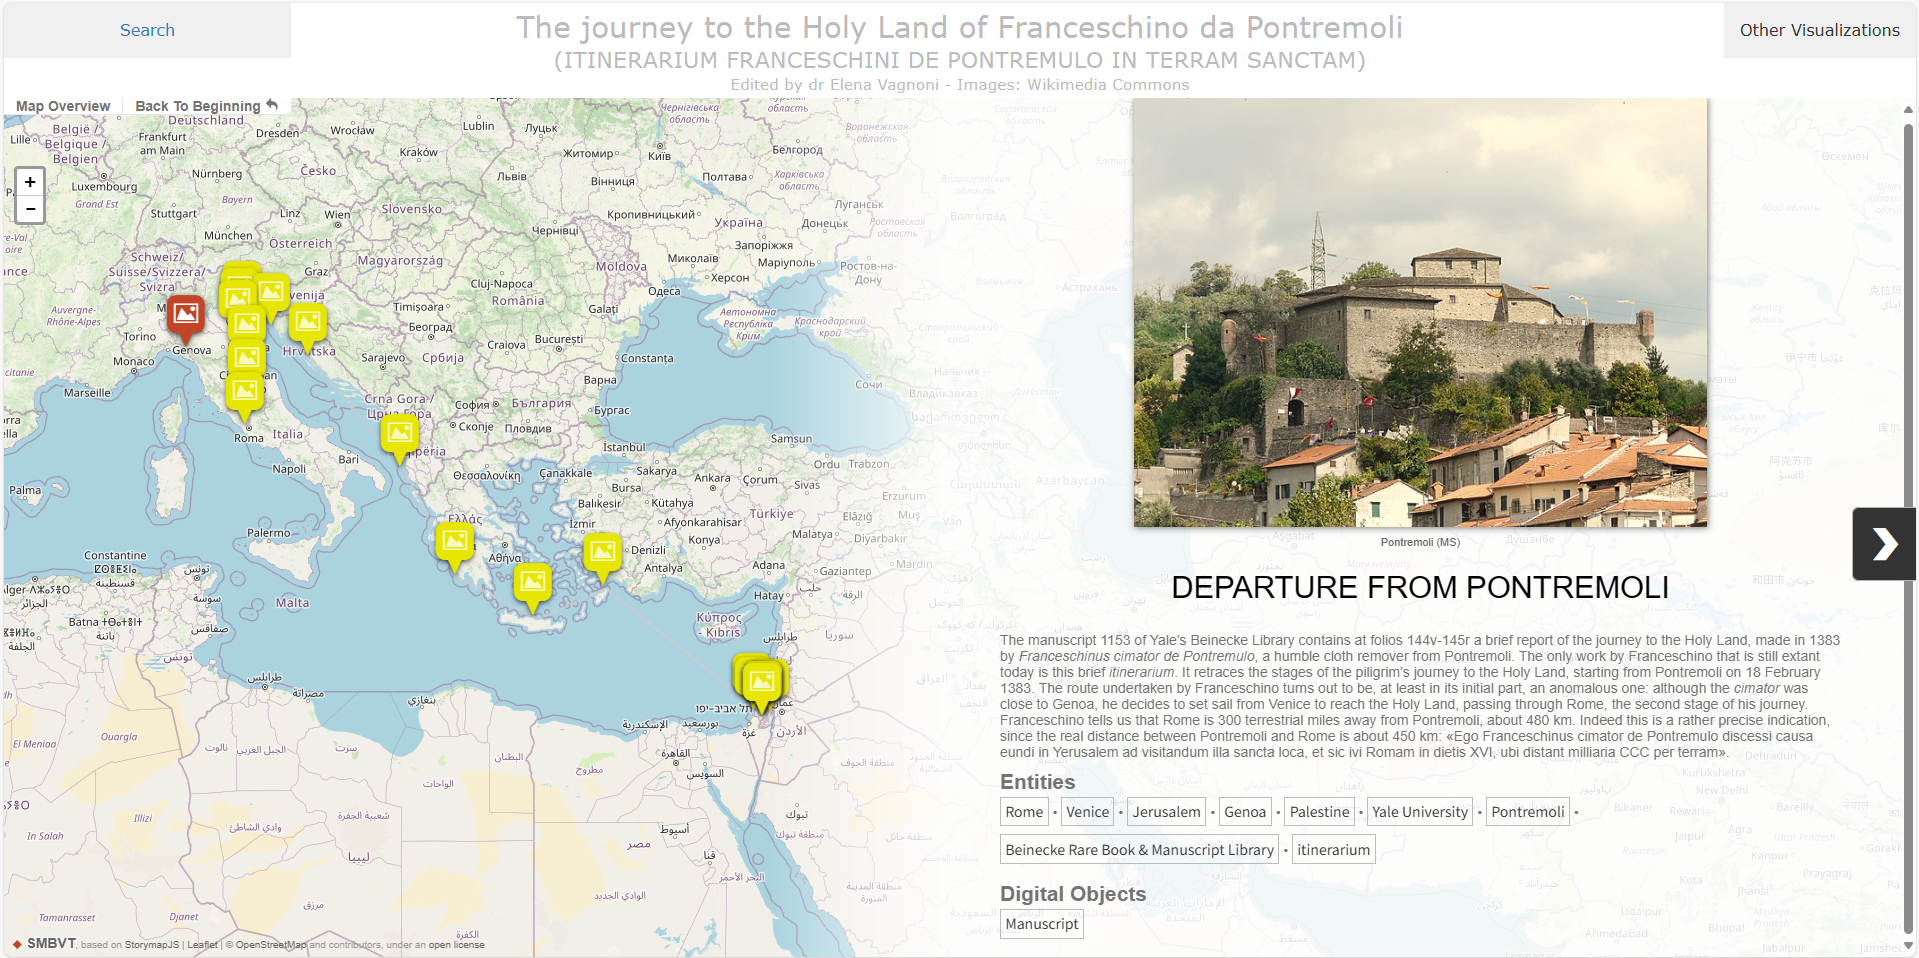
\includegraphics[scale=0.3]{img/franceschinoOverview.png}
    \caption{Overview of the Story Map "The Journey to the Holy Land of Franceschino da Pontremoli"}
    \label{fig:franceschino}
\end{figure}


This visualization technique aligns particularly well with the depiction of journeys or travels, as it effectively illustrates the trajectory of a journey by employing pins to denote key stages. A compelling historical instance of this approach is the pilgrimage to the Holy Land undertaken in 1383 by Franceschinus cimator de Pontremulo, a humble cloth remover from Pontremoli. The details of this pilgrimage are preserved in manuscript 1153 at Yale’s Beinecke Library, which documents the stages of Franceschino's pilgrimage, beginning in Pontremoli on February 18, 1383. The route taken by Franceschino is notable, particularly in its early phases, for its deviation from expected paths: despite the proximity of Pontremoli to Genoa, Franceschino chose to embark from Venice. This decision necessitated a detour through Rome, marking it as the second stage of his pilgrimage before proceeding to the Holy Land. The unique nature of Franceschino's path is vividly depicted in \Cref{fig:franceschino}, where each pin signifies a specific stage. By leveraging the story map, viewers can trace Franceschino’s journey interactively, gaining a narrative-driven exploration. Each stage is further enriched by contextual information, including associated participants, locations, and events. Such a graph structure can be queried to yield new insights, revealing connections otherwise obscured by the linear progression of text.


\begin{figure}[h!tb]
    \centering
    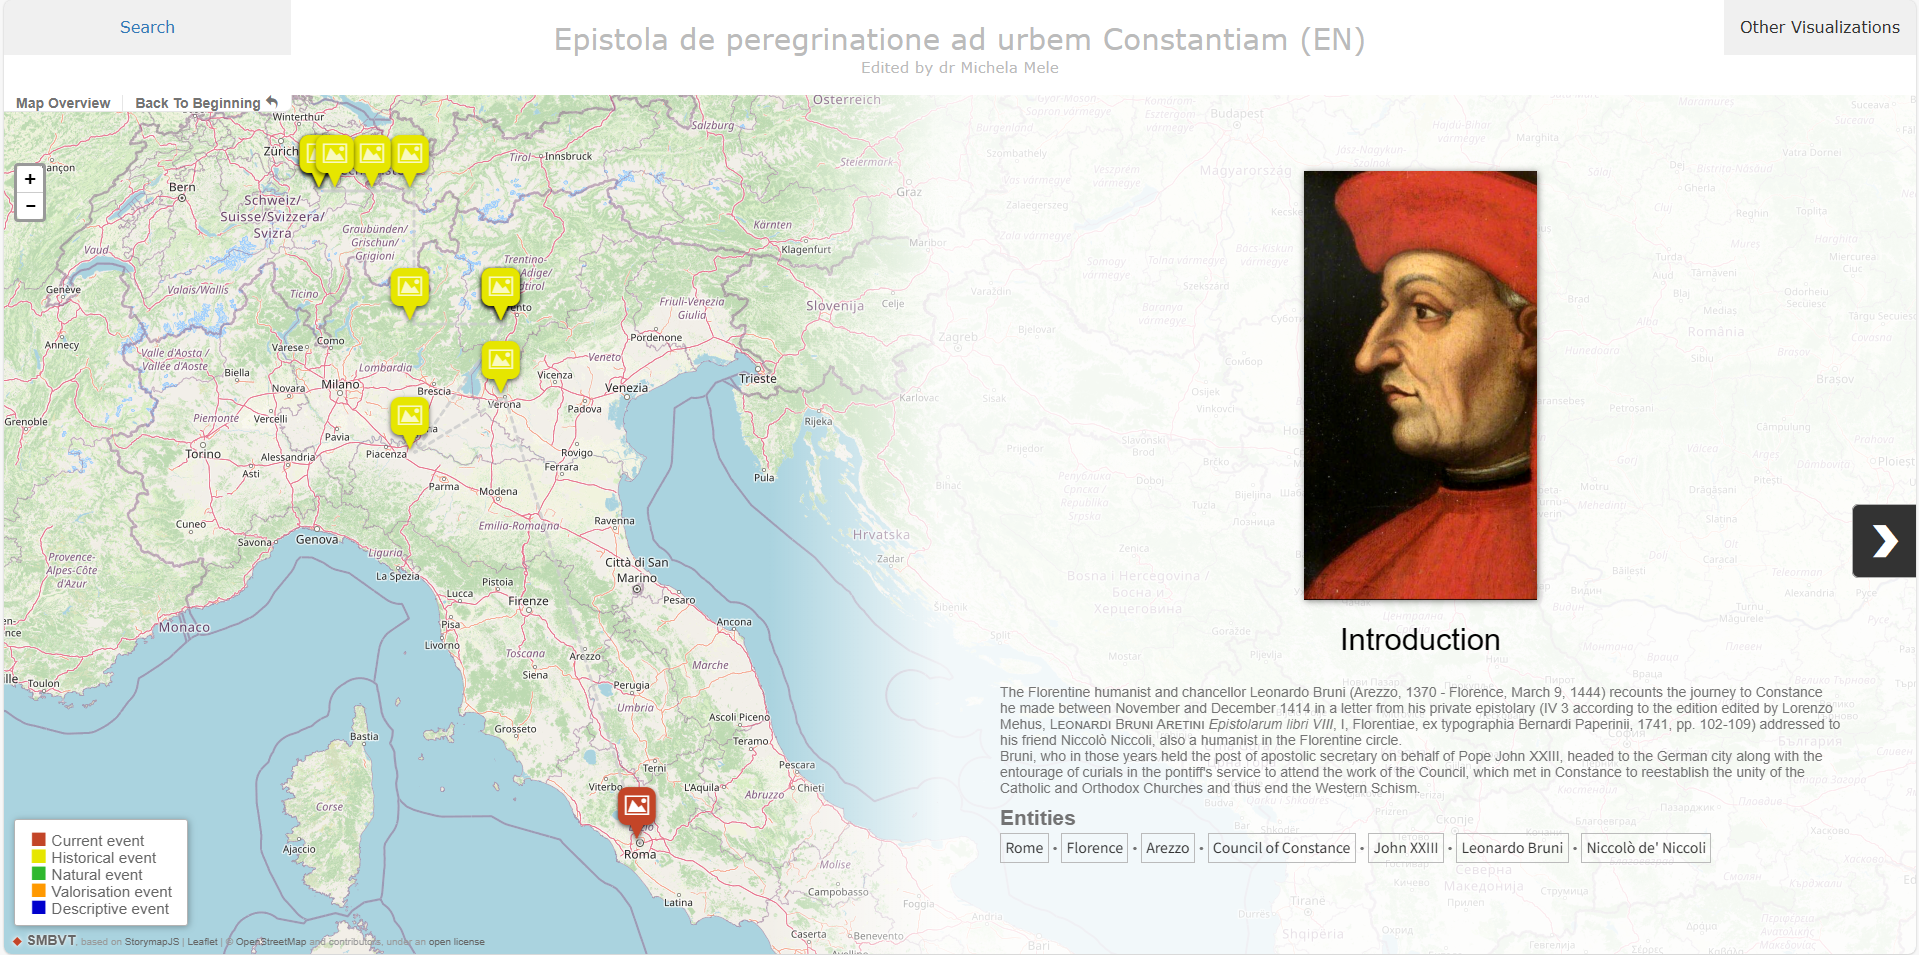
\includegraphics[scale=0.3]{img/bruniOverview.png}
    \caption{Overview of the Story Map "Epistola de peregrinatione ad urbem Constantiam"}
    \label{fig:bruni}
\end{figure}


In contrast, \Cref{fig:bruni} illustrates another significant journey: the voyage to Constance undertaken by the Florentine humanist and chancellor, Leonardo Bruni (1370–1444). Bruni recounts this journey, which occurred between November and December 1414, in a letter addressed to his friend Niccolò Niccoli, a fellow humanist within the Florentine intellectual circle. At the time, Bruni served as apostolic secretary to Pope John XXIII, travelling with the papal entourage to participate in the Council of Constance. This council aimed to reunify the Catholic and Orthodox Churches and bring an end to the Western Schism. Although Bruni's route is less immediately discernible compared to Franceschino's pilgrimage, the visual representation of the journey stages, marked as distinct events, remains highly informative. 

Employing SPARQL and GeoSPARQL queries on this knowledge graph offers a robust framework for discovering nuanced insights into Bruni's experiences. For instance, a notable anecdote emerges from Bruni’s fascination with the viticultural heritage of Termeno sulla Strada del Vino. As he travelled, he was struck by the region’s vineyards and the striking, the almost snowy appearance of the soil, which continues to yield the renowned white wine of Tramin, celebrated worldwide. This observation is not merely a historical curiosity; by integrating Bruni’s reflections with the \acrshort{MOVINGLabel} knowledge graph, one can draw connections across centuries, enriching our understanding of cultural and economic continuities within the winemaking tradition. The ability to query such structured information facilitates a multi-layered exploration, revealing insights that span both geographical and temporal dimensions.

\section{Discussion and Comparative Analysis}\label{VII-sec:discussion}

The interdisciplinary evaluation of NOnt+S, as applied to the \acrshort{MOVINGLabel} and \acrshort{IMAGOLabel} projects, provides critical insights into the ontology’s adaptability and effectiveness in modeling knowledge across varied, domain-specific contexts. This section offers a detailed exploration of NOnt+S’s performance, examining both its strengths and limitations in addressing the multifaceted needs of the bioeconomy and historical geography domains. The analysis not only emphasizes the ontology’s robustness in handling diverse semantic structures but also reflects on the broader implications for future applications in knowledge representation.

Within the \acrshort{MOVINGLabel} project, NOnt+S demonstrated remarkable proficiency in encapsulating the intricacies of bioeconomy and sustainability, particularly in mountain regions. The ontology’s flexible architecture facilitated the accurate representation of interconnected concepts such as agricultural practices, environmental conditions, and socio-economic dynamics. A major asset of NOnt+S was its capacity to integrate seamlessly with external geospatial datasets, including GISCO and \acrshort{OSMLabel}, thereby enhancing the granularity and accuracy of spatial data representations. This seamless integration allowed for comprehensive geospatial analysis, leveraging GeoSPARQL to perform sophisticated spatial queries. The modularity of the ontology proved to be instrumental in enriching domain-specific knowledge while maintaining compatibility with existing data standards. Nevertheless, the project also revealed areas where NOnt+S required further development. Specifically, the representation of specialized domains necessitated significant ontology customizations, which, while effective for the \acrshort{MOVINGLabel} project, introduced complexities that could hinder scalability and general applicability in broader or less uniform domains.

Turning to the \acrshort{IMAGOLabel} project, NOnt+S’s capacity to manage geospatial data within historical contexts emerged as a central strength. The ontology adeptly modeled place references derived from medieval texts, supporting in-depth analyses of geographic literature and the complex itineraries of medieval journeys. By leveraging external data repositories such as Wikidata and Pleiades, NOnt+S enriched historical geospatial information, demonstrating its versatility in addressing both temporal and spatial variability. However, the \acrshort{IMAGOLabel} project exposed unique challenges related to temporal alignment. Representing data across multiple, non-uniform historical periods required an intricate approach to ensure temporal consistency, complicating the ontology’s management of historical accuracy and logical coherence. The complexity of aligning medieval geographic concepts with modern data schemas imposed additional demands on data validation, requiring continuous monitoring to maintain semantic integrity.

Both projects utilized NOnt+S to facilitate the creation of structured knowledge graphs and enhance data visualization through Story Maps. These Story Maps were pivotal in narratively engaging users, weaving spatial references into a coherent visual exploration of medieval travel narratives. This method provided an intuitive interface for both academic researchers and the general public, making the historical data accessible and engaging. The success of Story Maps highlighted NOnt+S’s potential for transforming static historical and geographical data into dynamic, interactive experiences. Despite this, the projects also underscored the inherent complexity in ensuring uniform data integration when sourcing information from multiple, heterogeneous datasets. Addressing these complexities remains an area for future enhancement, suggesting that advancements in automated data alignment and refinement would be crucial for extending NOnt+S’s adaptability.

The comparative analysis of NOnt+S across the \acrshort{MOVINGLabel} and \acrshort{IMAGOLabel} projects illustrates the ontology’s significant potential for interdisciplinary applications, particularly in domains where narrative structures intersect with spatial data. Its adherence to Linked Open Data principles and standards-based design positions NOnt+S as a critical tool for facilitating cross-domain knowledge integration. Nevertheless, the ontology’s ability to scale and adapt to increasingly specialized and complex knowledge domains remains a challenge. To address these limitations, future iterations of NOnt+S may require refined support mechanisms for managing intricate extensions, improving semantic consistency, and optimizing automated data integration processes. Thus, while NOnt+S has proven its versatility and robustness, the evaluation also indicates pathways for further refinement, emphasizing the ontology’s continuous evolution to meet the demands of even more diverse and specialized research landscapes.

\subsection{Comparative Analysis of NOnt+S with Existing Ontologies and Representation Techniques}

The representation of narratives and their associated geospatial and temporal dimensions has emerged as a critical concern within knowledge modeling and digital humanities. In the previous Chapters we introduced the NOnt+S ontology, as an extension of the Narrative Ontology (NOnt), builds upon existing frameworks to address the challenges of integrating spatial semantics into narrative representation. Now we intend to introduce a thorough comparative analysis of NOnt+S against existing ontologies and knowledge representation approaches. Each comparison highlights the unique contributions of NOnt+S in addressing the limitations of earlier models.

The \Cref{table:comparative_analysis} summarizes the key features, strengths, and limitations of NOnt+S in comparison with existing ontologies and approaches.

\begin{table}[h!]\label{table:comparative_analysis}
\centering
\caption{Comparison of NOnt+S with Existing Ontologies and Techniques}
\label{tab:comparison}
 \scalebox{0.85}{
\begin{tabular}{|>{\raggedright}p{4cm}|>{\raggedright}p{4cm}|>{\raggedright}p{4cm}|>{\raggedright\arraybackslash}p{4cm}|}
\hline
\textbf{Ontology/Technique} & \textbf{Focus} & \textbf{Strengths} & \textbf{Limitations Overcome by NOnt+S} \\
\hline
CIDOC CRM & Event-based cultural heritage & Robust event and relationship modeling & Lacks explicit geospatial semantics and reasoning capabilities. \\
\hline
Narrative Cartography & Visual storytelling through maps & Spatio-temporal visualization of narratives & Static; lacks computational reasoning and semantic formalization. \\
\hline
InTaVia & Post-anthropocentric storytelling & Supports multiple narrative entities and visualization & No formal reasoning; lacks geospatial querying and semantic interoperability. \\
\hline
Ciotti's Formal Ontology & Narrative components: characters, traits, and spaces & Formal OWL-based representation of narrative semantics & Focused on textual abstraction; lacks spatial semantics and reasoning. \\
\hline
% \textbf{NOnt+S} & Narrative, geospatial, and temporal representation & Integrates geospatial semantics, formal reasoning, and advanced querying & Combines strengths of other approaches while addressing their limitations. \\
% \hline
\end{tabular}
}
\end{table}

As discussed in \Cref{III-subsec:cidoccrm}, the CIDOC CRM serves as a widely endorsed framework for modeling cultural heritage data, emphasizing the temporal and relational dynamics between entities. Its robust ontology provides a solid foundation for organizing historical and event-based knowledge, effectively supporting the mapping of cultural narratives. However, while CRM excels in modeling event-centric relationships, its capacity to capture the nuanced spatial semantics critical for geospatial narratives remains limited. The CRMgeo extension addresses this limitation by incorporating geospatial data modeling capabilities, yet it falls short of comprehensively representing narratives with detailed spatial semantics and reasoning capabilities. NOnt+S emerges as a solution to this challenge by extending the capabilities of CRM to explicitly integrate narrative structures and geospatial reasoning. Utilizing GeoSPARQL and OWL 2 DL, NOnt+S formalizes both qualitative and quantitative spatial relationships, enabling them to be computationally analyzed and reasoned upon. By embedding geospatial concepts such as proximity, topological relationships, and distances within a narrative framework, NOnt+S bridges the gap left by CRMgeo, facilitating a richer and more dynamic approach to geospatial narratives that supports advanced querying and inferential processes.

Narrative cartography, as conceptualized by scholars such as Caquard and Cartwright\cite{caquardNarrativeCartographyMapping2014}, highlights the interplay between spatial representation and storytelling, focusing on how maps can encapsulate the temporal, emotional, and ambiguous aspects of narratives. Traditional cartographic approaches, however, often rely on static visualizations and manually integrated spatial data, limiting their potential for computational analysis. NOnt+S revolutionizes narrative cartography by embedding it within a formal semantic framework, transforming static maps into dynamic, machine-readable representations. This approach enables the encoding of spatial and narrative data in formats that support automated reasoning and querying, uncovering hidden patterns and relationships within geospatial narratives. Through the use of OWL 2 DL, NOnt+S enables sophisticated inferential capabilities, which allow researchers to move beyond visualization and into deeper analytical understanding. By formalizing the spatial semantics of narratives, NOnt+S transcends the limitations of conventional narrative cartography, offering tools to dynamically explore and infer the complexities of geospatial storytelling.

Interactive platforms like InTaVia \cite{kusnickEveryThingCan2024} represent a significant innovation in the domain of cultural heritage and digital humanities by integrating visualization, data retrieval, and storytelling into cohesive, user-friendly interfaces. These platforms excel in constructing dynamic narratives that incorporate diverse entities, such as individuals, artifacts, locations, and institutions, and challenge anthropocentric biases by foregrounding the roles of non-human actors. Through interactive visualizations, InTaVia fosters an immersive user experience, enabling the exploration of complex relationships within cultural narratives. However, while platforms like InTaVia are highly effective at visualizing and integrating heterogeneous data, they lack the formal reasoning mechanisms required for deeper computational analysis. NOnt+S addresses this gap by embedding narratives within a semantically rich framework, integrating geospatial semantics with OWL 2 DL and GeoSPARQL to enable advanced reasoning and querying capabilities. This approach not only complements the visualization strengths of platforms like InTaVia but also facilitates a more profound analytical understanding of spatial narratives, bridging the divide between interactive visualization and formal computational analysis.

Fabio Ciotti's formal ontology for narrative \cite{ciottiFormalOntologyNarrative2016} represents a significant contribution to computational narratology, drawing upon semiotic and structuralist traditions to conceptualize narrative elements in machine-readable formats. Building on the theories of scholars like Greimas and Lotman, Ciotti formalizes key narrative components, including characters, traits, and spaces, using OWL 2 to represent these constructs systematically. His ontology emphasizes the dual roles of characters as actors and functional entities, inspired by Greimas' actantial model, allowing for the systematic analysis of their actions, traits, and relationships within a narrative structure. Additionally, Ciotti integrates Lotman's concept of semiotic space to model the interactions between characters and their narrative environments, offering a robust framework for textual analysis. Despite its innovative approach, Ciotti's ontology remains focused on abstract narrative structures, with limited engagement in geospatial reasoning. NOnt+S builds on Ciotti's conceptual foundation by incorporating the spatial and temporal dimensions of narratives, leveraging GeoSPARQL and OWL 2 DL to enable advanced geospatial querying and reasoning. This integration enhances the narrative framework by aligning textual semantics with spatial analytics, providing a comprehensive platform for analyzing, visualizing, and reasoning about complex geospatial narratives. In doing so, NOnt+S not only extends the analytical depth of formal ontologies but also positions itself as a pioneering tool for bridging narrative semantics and geospatial representation.


NOnt+S advances the state of narrative modeling by combining semantic reasoning, geospatial querying, and narrative formalization into a unified framework. Unlike earlier approaches, such as CIDOC CRM, knowledge graphs, and narrative cartography, NOnt+S explicitly integrates spatial semantics, ensuring that geospatial relationships can be formally represented and reasoned upon. While platforms like InTaVia prioritize visualization and interaction, NOnt+S provides the formal structure necessary for computational querying and inference. By incorporating spatial semantics, NOnt+S builds upon Fabio Ciotti's formal ontology, extending its narrative modeling capabilities into the geospatial domain. This ontology sets a new standard for narrative knowledge representation, bridging the gap between visualization, reasoning, and semantic interoperability.

\subsection{Adapting the NOnt+S Framework to Other Domains}

The NOnt+S framework demonstrates significant potential for adaptation across a range of domains, leveraging its strengths in semantic modeling, modular design, and querying capabilities. By addressing domain-specific challenges while maintaining general applicability, NOnt+S can be extended to meet the demands of diverse research and application areas. Below, we present a detailed exploration of considerations and enhancements required for such adaptations.
The modular architecture of NOnt+S, which has already proven effective in domains such as bioeconomy and geographic literature, can be generalized to suit broader applications. This requires separating foundational modules for semantic modeling, encompassing temporal, spatial, and narrative elements, from domain-specific extensions. Such a separation ensures that the core ontology remains reusable and flexible, while domain adapters or plugins can interface with specialized vocabularies and taxonomies. For instance, in the healthcare domain, NOnt+S could incorporate clinical narratives, such as patient journeys and treatment pathways, while linking geospatial data to public health studies, maybe with the integration of established biomedical ontologies.
Linking NOnt+S to domain-specific and open knowledge bases is essential for enriched data representation in areas such as urban planning or climate science. This integration involves using specialized datasets, such as Urban Atlas for urban planning or IPCC reports for climate change, and employing dynamic linking mechanisms. Automated enrichment processes can map NOnt+S entities to resources like GeoNames or domain-specific extensions of Wikidata, enabling seamless access to comprehensive and authoritative information. Such enhancements ensure that NOnt+S can support intricate narratives while maintaining alignment with evolving knowledge repositories.
While NOnt+S already supports advanced querying via GeoSPARQL and SPARQL, certain domains may require additional enhancements. Historical and archaeological applications, for example, demand temporal reasoning to model and query ancient events and their progression over time. Similarly, domains like environmental science or economics could benefit from causal and probabilistic reasoning to analyze relationships within complex datasets. These extensions would allow NOnt+S to address sophisticated research questions, expanding its analytical scope and utility.
Different domains exhibit unique user interaction requirements, necessitating customizable interfaces for the NOnt+S framework. In healthcare, visual dashboards can track real-time patient data and enable predictive modeling. Education could benefit from interactive story maps to support curriculum design, while social sciences might require tools for visualizing social networks and relationships. By incorporating user-centric design principles, NOnt+S can enhance accessibility and usability, fostering adoption across diverse fields.
Certain domains, such as cultural heritage preservation or biomedicine, necessitate careful attention to ethical and cultural factors. Incorporating modules for ethical reasoning, such as those ensuring compliance with data privacy and consent requirements, is essential. Similarly, the framework should adapt ontological representations to account for cultural variations, particularly in global projects. These considerations enhance the relevance and sensitivity of NOnt+S in diverse sociocultural contexts.
The flexibility of NOnt+S opens opportunities for applications in emerging domains. In artificial intelligence ethics, the framework could model decision-making narratives to ensure transparency and accountability. For space exploration, NOnt+S can represent interplanetary missions, facilitating reasoning about extraterrestrial geospatial data. Additionally, the gaming and entertainment industry could utilize NOnt+S to structure interactive narratives for virtual environments, offering innovative solutions for immersive storytelling.


\section{Conclusion}\label{VII-sec:conclusion}

The interdisciplinary evaluation of the NOnt+S ontology across bioeconomy studies and geographic literature has demonstrated its effectiveness in modeling domain-specific knowledge while maintaining flexibility and extensibility. Through its modular structure, NOnt+S was able to accommodate diverse concepts, ranging from resource management in the bioeconomy to spatial relations in geographic literature.

The application of the framework presented in the \textit{Framework} chapter has further validated NOnt+S as a robust ontology for interdisciplinary research. Future work will focus on addressing the identified challenges, particularly concerning the integration of highly specialized concepts and ensuring consistent data validation across even broader domains.


 
% \chapter{Discussion}

% \section{Overview of Contributions}

% This research advances the formal representation of geospatial knowledge in narratives through the development of the NOnt+S ontology, a geospatially extended framework built on the foundation of the existing Narrative Ontology (NOnt). The following discussion elaborates on the main contributions, strengths, and limitations of NOnt+S and explores the impact and future directions of this research.

% The primary achievement of this work lies in bridging the gap between the nuanced, narrative representation of geospatial elements and the need for structured, machine-readable data formats. Traditional ontologies have often struggled to accommodate the temporal and dynamic aspects of narratives, particularly when dealing with the inherent ambiguity and subjectivity of natural language. By integrating geospatial reasoning capabilities and adopting Semantic Web technologies, NOnt+S provides a robust solution to these challenges.

% \section{Analysis of Key Findings}

% The NOnt+S ontology is designed to model complex relationships between narrative events and spatial locations, facilitating efficient querying and reasoning. By extending NOnt to include geospatial elements, NOnt+S enhances the ability to represent both qualitative and quantitative spatial relationships. The introduction of geospatial reasoning, coupled with semantic reasoning, enables the inference of new spatial-temporal insights from narrative data. This dual capability represents a significant step forward in the computational analysis of narratives.

% \subsection{Effectiveness in Real-World Applications}

% The validation of NOnt+S through case studies in bioeconomy research and the study of medieval geographic literature demonstrates the ontology’s versatility. In the bioeconomy domain, the ontology's ability to enrich data with geospatial context enhances understanding of mountain ecosystems and facilitates interdisciplinary knowledge sharing. Similarly, in the cultural heritage domain, NOnt+S provides a structured way to explore complex narrative journeys, such as those depicted in medieval manuscripts, revealing patterns and connections that were previously difficult to identify.

% Furthermore, the visualization tool, Story Maps, developed as part of this research, adds a significant dimension to narrative exploration. By representing temporal progression alongside spatial data, Story Maps make abstract relationships tangible and intuitive, supporting educational and research endeavors in digital humanities and beyond.

% \section{Comparative Strengths and Limitations}

% \subsection{Strengths}

% One of the major strengths of NOnt+S is its adherence to Semantic Web standards, which ensures interoperability and facilitates integration with other ontologies. The use of OWL2 DL ensures logical consistency, while the incorporation of established frameworks like CIDOC CRM and GeoSPARQL enhances the ontology's applicability across multiple domains. The ontology’s design also emphasizes flexibility, allowing for future extensions to address domain-specific requirements.

% The semantic reasoner and geospatial reasoning mechanisms embedded within NOnt+S significantly enhance its analytical capabilities. These features enable the ontology to infer implicit knowledge, such as identifying recurring spatial patterns or understanding the movement of characters within a narrative. This dual-layered reasoning capability distinguishes NOnt+S from traditional narrative ontologies, which often lack comprehensive spatial reasoning.

% \subsection{Limitations}

% Despite these strengths, NOnt+S does face certain limitations. Scalability remains a concern, as extending the ontology to cover a wide array of domains may require significant customization. The integration of heterogeneous data sources also presents challenges; data from different origins often lack semantic coherence and may require extensive pre-processing. Furthermore, the ontology's current representation of spatiotemporal relationships, though advanced, struggles with highly dynamic datasets, and computational complexity increases significantly with large-scale narratives.

% The visualization component, while effective, may not fully capture the intricacies of complex spatial narratives. Although Story Maps provide an interactive and engaging means of exploration, the interpretive nature of narratives means that some spatial relationships may be oversimplified or misrepresented.

% \section{Implications for Future Research}

% The limitations identified in this study offer opportunities for future research. Addressing the ontology's scalability will require developing specialized extensions tailored to diverse domains, as well as optimizing data integration workflows. Further, enhancing NOnt+S's temporal reasoning capabilities, such as refining temporal primitives and exploring more efficient spatiotemporal representation methods, is a priority for future iterations.

% Incorporating Natural Language Processing (NLP) modules for automated narrative extraction could significantly improve the ontology's usability, particularly in dealing with unstructured text. By integrating tools that can parse and annotate narratives with geospatial tags, NOnt+S could automate much of the data pre-processing currently required. Additionally, exploring new data formats, such as GeoJSON and the forthcoming updates to GeoSPARQL 1.1, could improve the ontology's compatibility and ease of use.

% \section{Conclusion}

% In summary, NOnt+S represents a comprehensive advancement in the field of geospatial narrative representation. By addressing the limitations of traditional ontologies and offering new avenues for narrative exploration through Semantic Web technologies, this research lays the groundwork for future developments in both the digital humanities and scientific domains. While challenges remain, the potential for further refinement and application of this ontology is vast, paving the way for more sophisticated, integrated approaches to understanding and visualizing geospatial knowledge in narratives.
 
\chapter{Conclusion}\label{chap:conclusion}

\section{Summary of Findings}

This research introduced and thoroughly evaluated the \acrfull{NOnt+SLabel} ontology, a specialized framework designed to semantically represent geospatial knowledge within narrative contexts. The ontology demonstrated notable adaptability and extensibility by implementing \acrshort{NOnt+SLabel} across various interdisciplinary domains—such as bioeconomy and medieval geographical literature. The findings indicate that \acrshort{NOnt+SLabel} successfully models complex spatial and thematic relationships, thereby fulfilling the research objectives and establishing itself as a robust framework that unifies geospatial and narrative dimensions. One of the standout features of \acrshort{NOnt+SLabel} is its modular architecture, which allows for customization to meet the specific demands of diverse fields. For instance, in the bioeconomy, ontology facilitated the representation of value chains, while in historical geography, it provided tools for modelling intricate spatial-temporal relationships. This adaptability underlines the ontology’s potential as a comprehensive and flexible resource for managing geospatial narratives across disciplines.

\section{Contributions to Knowledge}

This study advances the field of geospatial narrative ontology, particularly in digital libraries, by developing the \acrshort{NOnt+SLabel} ontology — a framework that integrates narrative and spatial elements to model complex, layered narratives. \acrshort{NOnt+SLabel} innovatively combines narrative structures, such as \textit{fabula} (chronological story sequence) and \textit{syuzhet} (narrative presentation), with spatial constructs like qualitative and quantitative places. By bridging narrative and spatial dimensions, \acrshort{NOnt+SLabel} fills a critical gap in conventional ontologies, which often struggle to represent multifaceted narrative-spatial relationships. This framework thus sets a new standard for flexible and comprehensive modelling, applicable across diverse scientific domains that require sophisticated geospatial narrative representation.

To ensure interoperability and ease of integration, \acrshort{NOnt+SLabel} adopts established standards such as the CIDOC CRM, an ISO-standard vocabulary used extensively in cultural heritage. Extending this vocabulary promotes compatibility with existing ontological frameworks, enabling \acrshort{NOnt+SLabel} to integrate seamlessly with established data systems and legacy structures. Additionally, adherence to GeoSPARQL standards ensures that \acrshort{NOnt+SLabel} can handle complex geospatial queries while remaining compatible with semantic web technologies, further enhancing its adaptability across varied applications.

A pivotal feature of \acrshort{NOnt+SLabel} is its embedded semantic reasoner, which enables the inference of new knowledge based on existing data. This reasoning mechanism allows the ontology to uncover hidden patterns and relationships within narrative and spatial data, generating insights that may otherwise remain undetected. By enhancing knowledge depth and applicability, \acrshort{NOnt+SLabel} offers a valuable tool for research fields that require nuanced understanding of narrative-geospatial relationships. The ontology’s open science-oriented approach also supports transparency and broad accessibility, encouraging collaborative research and facilitating its adoption across the research community.

In addition to these structural and semantic advancements, this study developed a software architecture that visualizes knowledge through Story Maps. Story Maps provide an intuitive, narrative-driven interface for exploring geospatial narratives, integrating text, images, and maps into cohesive visual stories. This visualization capability enables a deeper, more immersive user experience, facilitating understanding of complex narrative and spatial interrelationships. Story Maps thus extend the utility of \acrshort{NOnt+SLabel} by offering an accessible, interactive platform that supports researchers, educators, and professionals in analyzing geospatial narratives.

This research introduces methodological innovations to support the construction of structured geospatial knowledge graphs, enabling more efficient data interoperability and visualization. By embedding reasoning mechanisms and aligning with Linked Open Data (LOD) principles, \acrshort{NOnt+SLabel} ensures data reusability and broad compatibility across fields. Its standards-compliant design positions \acrshort{NOnt+SLabel} as a robust, adaptable tool that supports interdisciplinary collaborations in areas such as digital humanities and bioeconomy, where complex geospatial narrative modeling is essential.

Validated across diverse research contexts, \acrshort{NOnt+SLabel} demonstrates effectiveness in managing intricate geospatial queries and representing narrative structures. Its versatility highlights its potential as a foundational tool within the semantic web landscape, serving as a significant asset for advanced geospatial narrative modeling and supporting the future of narrative representation across domains.

\section{Limitations}

While \acrshort{NOnt+SLabel} has proven to be robust and flexible, certain limitations emerged during its application in diverse domains. One notable limitation pertains to domain-specific scalability. Although the ontology’s modular structure provides a degree of flexibility, the need for specialized extensions to fully capture certain domain-specific complexities may impact scalability when applying the ontology across highly varied fields. This challenge underscores the need for ongoing refinement to ensure that the ontology remains adaptable without compromising its core structure or functionality.

Data integration presented another challenge, especially when dealing with heterogeneous data sources characterized by varying levels of granularity. Ensuring consistency and semantic coherence across these sources proved difficult, emphasizing the need for additional refinements to improve compatibility with diverse data structures. Furthermore, \acrshort{NOnt+SLabel} encountered limitations in representing certain aspects of geospatial data, particularly with respect to managing complex spatial-temporal relationships. While the ontology supports standard geospatial formats, constraints in dynamic temporal representation may restrict its effectiveness in applications involving rapidly evolving datasets. Addressing these limitations is essential for enhancing \acrshort{NOnt+SLabel}’s capability to operate seamlessly across dynamic and varied research contexts.

\section{Future Work}
In light of the contributions and limitations identified, several promising directions for future research are proposed. 

\subsection{Model Extention}
Enhancing the geospatial data modeling capabilities of \acrshort{NOnt+SLabel} is a primary focus. By integrating new geospatial data formats, such as GeoJSON, alongside advancements from GeoSPARQL 1.1 \cite{carGeoSPARQL11Motivations2022}, \acrshort{NOnt+SLabel} could achieve greater interoperability, broadening its applicability within dynamic data contexts. This integration would expand the ontology’s ability to represent a wider array of geospatial data types, making it more compatible with modern geospatial systems and increasing its relevance in diverse applications.

\subsection{Integration with Large Language Models}

Large Language Models (LLMs), such as ChatGPT\cite{ChatGPT}, have demonstrated remarkable capabilities in generating coherent and contextually relevant text. However, their performance is often undermined by the hallucination problem, which manifests as a tendency to produce content that is factually inaccurate or logically inconsistent, especially when dealing with structured data or complex reasoning tasks. The integration of NOnt+S with LLMs presents an opportunity to mitigate these shortcomings, particularly in scenarios requiring precise geospatial and temporal reasoning. For instance, by employing NOnt+S, it becomes feasible to cross-reference generated narratives with an established framework to ensure factual accuracy. An illustrative example of this would be an LLM suggesting that "Event X occurred in Location Y during 1200 CE"; through NOnt+S, the system could validate whether "Location Y" indeed existed during the specified period and assess its spatial relevance to other referenced locations. This validation mechanism enhances the reliability of generated content by aligning it with ontological data.

Furthermore, advancements in the automatic segmentation of text into events\cite{bartalesiUsingLargeLanguage2024} provide a foundational layer for integrating such capabilities. This segmentation process enables LLMs to decompose narratives into discrete components, which can then be systematically mapped to ontology classes and properties through natural language processing techniques. By bridging unstructured text with structured ontological data, this integration allows for a dynamic feedback loop, wherein LLMs refine their outputs based on real-time ontology-driven validations. Central to this approach is the use of SPARQL endpoints, which facilitate the querying and retrieval of structured knowledge from NOnt+S knowledge graphs. This bidirectional interaction not only enhances the factual reliability of LLM outputs but also underscores the potential of ontology-based systems in augmenting the functionality and trustworthiness of large-scale language models.


\subsection{Validation in Other Domains}
Further interdisciplinary validation is also planned, particularly within the CRAEFT \cite{CraeftCareJudgment} and ECHOES \cite{EchoesEccchEuropean} projects. These projects aim to apply \acrshort{NOnt+SLabel} to represent geospatial knowledge related to traditional European craft and cultural heritage, respectively. Such applications will extend the ontology’s interdisciplinary relevance, reinforcing its capability to meet the demands of various research domains. This planned validation across different fields will not only improve the ontology’s practical applicability but also deepen its theoretical grounding, thereby broadening its scope for future use.



\section{Conclusion}

In conclusion, the evaluation and validation of the \acrshort{NOnt+SLabel} ontology have demonstrated its applicability across multiple domains and its potential for generating new insights through semantic reasoning. By bridging narrative and geospatial knowledge representation, \acrshort{NOnt+SLabel} offers a robust framework capable of handling complex spatial narratives. While there are areas for refinement—particularly concerning scalability and data integration—the ontology’s contributions underscore its significant value to interdisciplinary research. The planned expansions of the ontology, including the incorporation of additional geographic formats and ongoing use in interdisciplinary projects, indicate a promising future. \acrshort{NOnt+SLabel} stands as a versatile tool, offering substantial contributions to the semantic web landscape by enabling the representation and analysis of geospatial knowledge across a wide range of research fields. With continued development and interdisciplinary applications, \acrshort{NOnt+SLabel} has the potential to become a foundational resource within the domain of geospatial knowledge representation, supporting more comprehensive and nuanced approaches to digital knowledge management.
 

\appendix

% \chapter{NOnt+S Ontology with OWL Manchester Syntax}

% \begin{lstlisting}
% Prefix: : <https://dlnarratives.eu#>
% Prefix: crmgeo: <https://dlnarratives.eu/crmgeo/>
% Prefix: crminf: <https://dlnarratives.eu/crminf/>
% Prefix: current: <http://erlangen-crm.org/current/>
% Prefix: geosparql: <http://www.opengis.net/ont/geosparql#>
% Prefix: ontology: <https://dlnarratives.eu/ontology#>
% Prefix: owl: <http://www.w3.org/2002/07/owl#>
% Prefix: rdf: <http://www.w3.org/1999/02/22-rdf-syntax-ns#>
% Prefix: rdfs: <http://www.w3.org/2000/01/rdf-schema#>
% Prefix: skos: <http://www.w3.org/2004/02/skos/core#>
% Prefix: xml: <http://www.w3.org/XML/1998/namespace>
% Prefix: xsd: <http://www.w3.org/2001/XMLSchema#>


% Ontology: <https://dlnarratives.eu>
% AnnotationProperty: rdfs:comment
% AnnotationProperty: rdfs:label
% AnnotationProperty: skos:notation
% Datatype: geosparql:gmlLiteral
% Datatype: geosparql:wktLiteral
% Datatype: rdf:PlainLiteral  
% Datatype: rdfs:Literal  
% Datatype: xsd:string  
% ObjectProperty: <http://erlangen-crm.org/efrbroo/R17i_was_created_by>  
% ObjectProperty: <http://www.w3.org/2006/time#after>
%     Domain: 
%         <http://www.w3.org/2006/time#Instant>    
%     Range: 
%         <http://www.w3.org/2006/time#Instant>  
%     InverseOf: 
%         <http://www.w3.org/2006/time#before>
      
% ObjectProperty: <http://www.w3.org/2006/time#before>
%     Characteristics: 
%         Transitive  
%     Domain: 
%         <http://www.w3.org/2006/time#Instant>,
%         <http://www.w3.org/2006/time#TemporalEntity>    
%     Range: 
%         <http://www.w3.org/2006/time#Instant>,
%         <http://www.w3.org/2006/time#TemporalEntity>    
%     InverseOf: 
%         <http://www.w3.org/2006/time#after>
    
% ObjectProperty: crmgeo:Q5_defined_in
%     Domain: 
%         current:E53_Place  
%     Range: 
%         crmgeo:SP3_Reference_Space
       
% ObjectProperty: crmgeo:Q7_describes
%     Domain: 
%         crmgeo:SP4_Spatial_Coordinate_Reference_System   
%     Range: 
%         crmgeo:SP3_Reference_Space   
    
% ObjectProperty: crmgeo:Q9_is_expressed_in_terms_of
    
% ObjectProperty: crminf:J1_was_premise_for
%     Domain: 
%         crminf:I2_Belief
%     Range: 
%         crminf:I5_Inference_Making
    
% ObjectProperty: crminf:J2_concluded_that
%     Domain: 
%         crminf:I5_Inference_Making
%     Range: 
%         crminf:I2_Belief 
    
% ObjectProperty: crminf:J4_that
%     Domain: 
%         crminf:I2_Belief
%     Range: 
%         crminf:I4_Proposition_Set
    
% ObjectProperty: crminf:O16_observed_value
%     Domain: 
%         crminf:S4_Observation
%     Range: 
%         crminf:I4_Proposition_Set
    
% ObjectProperty: crminf:O8_observed
%     Domain: 
%         crminf:S15_Observable_Entity
%     Range: 
%         crminf:S4_Observation
     
% ObjectProperty: current:P100_was_death_of 
% ObjectProperty: current:P104_is_subject_to 
% ObjectProperty: current:P105_right_held_by  
% ObjectProperty: current:P106_is_composed_of
%     Annotations: 
%         rdfs:comment "Scope note:
% This property associates an instance of E90 Symbolic Object with a part of it that is by itself an instance of E90 Symbolic Object, such as fragments of texts or clippings from an image. This property is transitive.

% Examples:
% - This Scope note P106 (E33) is composed of fragments of texts (E33)
% - 'recognizable' P106 (E90) is composed of 'ecognizabl' (E90)

% In First Order Logic:
% P106(x,y) ⊃ E90(x)
% P106(x,y) ⊃ E90(y)"@en,
%         rdfs:label "P106 is composed of"@en,
%         skos:notation "P106"
    
%     Characteristics: 
%         Transitive
    
%     Domain: 
%         current:E90_Symbolic_Object
    
%     Range: 
%         current:E90_Symbolic_Object
    
%     InverseOf: 
%         current:P106i_forms_part_of
    
    
% ObjectProperty: current:P106i_forms_part_of

%     Annotations: 
%         rdfs:label "P106 forms part of"@en,
%         skos:notation "P106i"
    
%     Characteristics: 
%         Transitive
    
%     Domain: 
%         current:E90_Symbolic_Object
    
%     Range: 
%         current:E90_Symbolic_Object
    
%     InverseOf: 
%         current:P106_is_composed_of
    
    
% ObjectProperty: current:P107_has_current_or_former_member

    
% ObjectProperty: current:P108_has_produced

    
% ObjectProperty: current:P110_augmented

    
% ObjectProperty: current:P111_added

    
% ObjectProperty: current:P112_diminished

    
% ObjectProperty: current:P113_removed

    
% ObjectProperty: current:P114_is_equal_in_time_to

%     Annotations: 
%         rdfs:comment "Scope note:
% This symmetric property allows the instances of E2 Temporal Entity with the same E52 Time-Span to be equated.
% This property is only necessary if the time span is unknown (otherwise the equivalence can be calculated).

% This property is the same as the \"equal\" relationship of Allen’s temporal logic (Allen, 1983, pp. 832-843).
% This property is transitive.

% Examples:
% - the destruction of the Villa Justinian Tempus (E6) is equal in time to the death of Maximus Venderus (E69)

% In First Order Logic:
% P114(x,y) ⊃ E2(x)
% P114(x,y) ⊃ E2(y)
% P114(x,y) ⊃ P114(y,x)"@en,
%         rdfs:label "P114 is equal in time to"@en,
%         skos:notation "P114"
    
%     Characteristics: 
%         Symmetric,
%         Transitive
    
%     Domain: 
%         current:E2_Temporal_Entity
    
%     Range: 
%         current:E2_Temporal_Entity
    
%     InverseOf: 
%         current:P114_is_equal_in_time_to
    
    
% ObjectProperty: current:P115_finishes

%     Annotations: 
%         rdfs:comment "Scope note:
% This property allows the ending point for a E2 Temporal Entity to be situated by reference to the ending point of another temporal entity of longer duration.

% This property is only necessary if the time span is unknown (otherwise the relationship can be calculated). This property is the same as the \"finishes / finished-by\" relationships of Allen’s temporal logic (Allen, 1983, pp. 832-843).
% This property is transitive.

% Examples:
% - Late Bronze Age (E4) finishes Bronze Age (E4)

% In First Order Logic:
% P115(x,y) ⊃ E2(x)
% P115(x,y) ⊃ E2(y)"@en,
%         rdfs:label "P115 finishes"@en,
%         skos:notation "P115"
    
%     Characteristics: 
%         Transitive
    
%     Domain: 
%         current:E2_Temporal_Entity
    
%     Range: 
%         current:E2_Temporal_Entity
    
%     InverseOf: 
%         current:P115i_is_finished_by
    
    
% ObjectProperty: current:P115i_is_finished_by

%     Annotations: 
%         rdfs:label "P115 is finished by"@en,
%         skos:notation "P115i"
    
%     Characteristics: 
%         Transitive
    
%     Domain: 
%         current:E2_Temporal_Entity
    
%     Range: 
%         current:E2_Temporal_Entity
    
%     InverseOf: 
%         current:P115_finishes
    
    
% ObjectProperty: current:P116_starts

%     Annotations: 
%         rdfs:comment "Scope note:
% This property allows the starting point for a E2 Temporal Entity to be situated by reference to the starting point of another temporal entity of longer duration.

% This property is only necessary if the time span is unknown (otherwise the relationship can be calculated). This property is the same as the \"starts / started-by\" relationships of Allen’s temporal logic (Allen, 1983, pp. 832-843).

% Examples:
% - Early Bronze Age (E4) starts Bronze Age (E4)

% In First Order Logic:
% P116(x,y) ⊃ E2(x)
% P116(x,y) ⊃ E2(y)"@en,
%         rdfs:label "P116 starts"@en,
%         skos:notation "P116"
    
%     Characteristics: 
%         Transitive
    
%     Domain: 
%         current:E2_Temporal_Entity
    
%     Range: 
%         current:E2_Temporal_Entity
    
%     InverseOf: 
%         current:P116i_is_started_by
    
    
% ObjectProperty: current:P116i_is_started_by

%     Annotations: 
%         rdfs:label "P116 is started by"@en,
%         skos:notation "P116i"
    
%     Characteristics: 
%         Transitive
    
%     Domain: 
%         current:E2_Temporal_Entity
    
%     Range: 
%         current:E2_Temporal_Entity
    
%     InverseOf: 
%         current:P116_starts
    
    
% ObjectProperty: current:P117_occurs_during

%     Annotations: 
%         rdfs:comment "Scope note:
% This property allows the entire E52 Time-Span of an E2 Temporal Entity to be situated within the Time-Span of another temporal entity that starts before and ends after the included temporal entity.

% This property is only necessary if the time span is unknown (otherwise the relationship can be calculated). This property is the same as the \"during / includes\" relationships of Allen’s temporal logic (Allen, 1983, pp. 832-843).

% Examples:
% - Middle Saxon period (E4) occurs during Saxon period (E4)

% In First Order Logic:
% P117(x,y) ⊃ E2(x)
% P117(x,y) ⊃ E2(y)"@en,
%         rdfs:label "P117 occurs during"@en,
%         skos:notation "P117"
    
%     Characteristics: 
%         Transitive
    
%     Domain: 
%         current:E2_Temporal_Entity
    
%     Range: 
%         current:E2_Temporal_Entity
    
%     InverseOf: 
%         current:P117i_includes
    
    
% ObjectProperty: current:P117i_includes

%     Annotations: 
%         rdfs:label "P117 includes"@en,
%         skos:notation "P117i"
    
%     Characteristics: 
%         Transitive
    
%     Domain: 
%         current:E2_Temporal_Entity
    
%     Range: 
%         current:E2_Temporal_Entity
    
%     InverseOf: 
%         current:P117_occurs_during
    
    
% ObjectProperty: current:P118_overlaps_in_time_with

%     Annotations: 
%         rdfs:comment "Scope note:
% This property identifies an overlap between the instances of E52 Time-Span of two instances of E2 Temporal Entity.

% It implies a temporal order between the two entities: if A overlaps in time B, then A must start before B, and B must end after A. This property is only necessary if the relevant time spans are unknown (otherwise the relationship can be calculated).

% This property is the same as the \"overlaps / overlapped-by\" relationships of Allen’s temporal logic (Allen, 1983, pp. 832-843).

% Examples:
% - the Iron Age (E4) overlaps in time with the Roman period (E4)

% In First Order Logic:
% P118(x,y) ⊃ E2(x)
% P118(x,y) ⊃ E2(y)"@en,
%         rdfs:label "P118 overlaps in time with"@en,
%         skos:notation "P118"
    
%     Domain: 
%         current:E2_Temporal_Entity
    
%     Range: 
%         current:E2_Temporal_Entity
    
%     InverseOf: 
%         current:P118i_is_overlapped_in_time_by
    
    
% ObjectProperty: current:P118i_is_overlapped_in_time_by

%     Annotations: 
%         rdfs:label "P118 is overlapped in time by"@en,
%         skos:notation "P118i"
    
%     Domain: 
%         current:E2_Temporal_Entity
    
%     Range: 
%         current:E2_Temporal_Entity
    
%     InverseOf: 
%         current:P118_overlaps_in_time_with
    
    
% ObjectProperty: current:P119_meets_in_time_with

%     Annotations: 
%         rdfs:comment "Scope note:
% This property indicates that one E2 Temporal Entity immediately follows another.

% It implies a particular order between the two entities: if A meets in time with B, then A must precede B. This property is only necessary if the relevant time spans are unknown (otherwise the relationship can be calculated).

% This property is the same as the \"meets / met-by\" relationships of Allen's temporal logic (Allen, 1983, pp. 832-843).

% Examples:
% - Early Saxon Period (E4) meets in time with Middle Saxon Period (E4)

% In First Order Logic:
% P119(x,y) ⊃ E2(x)
% P119(x,y) ⊃ E2(y)"@en,
%         rdfs:label "P119 meets in time with"@en,
%         skos:notation "P119"
    
%     Domain: 
%         current:E2_Temporal_Entity
    
%     Range: 
%         current:E2_Temporal_Entity
    
%     InverseOf: 
%         current:P119i_is_met_in_time_by
    
    
% ObjectProperty: current:P119i_is_met_in_time_by

%     Annotations: 
%         rdfs:label "P119 is met in time by"@en,
%         skos:notation "P119i"
    
%     Domain: 
%         current:E2_Temporal_Entity
    
%     Range: 
%         current:E2_Temporal_Entity
    
%     InverseOf: 
%         current:P119_meets_in_time_with
    
    
% ObjectProperty: current:P11_had_participant

%     Annotations: 
%         rdfs:comment "Scope note:
% This property describes the active or passive participation of instances of E39 Actors in an E5 Event.

% It connects the life-line of the related E39 Actor with the E53 Place and E50 Date of the event. The property implies that the Actor was involved in the event but does not imply any causal relationship. The subject of a portrait can be said to have participated in the creation of the portrait.

% Examples:
% - Napoleon (E21) participated in The Battle of Waterloo (E7)
% - Maria (E21) participated in Photographing of Maria (E7)

% In First Order Logic:
% P11(x,y) ⊃ E5(x)
% P11(x,y) ⊃ E39(y)
% P11(x,y) ⊃ P12(x,y)"@en,
%         rdfs:label "P11 had participant"@en,
%         skos:notation "P11"
    
%     SubPropertyOf: 
%         current:P12_occurred_in_the_presence_of
    
%     Domain: 
%         current:E5_Event
    
%     Range: 
%         current:E39_Actor
    
%     InverseOf: 
%         current:P11i_participated_in
    
    
% ObjectProperty: current:P11i_participated_in

%     Annotations: 
%         rdfs:label "P11 participated in"@en,
%         skos:notation "P11i"
    
%     SubPropertyOf: 
%         current:P12i_was_present_at
    
%     Domain: 
%         current:E39_Actor
    
%     Range: 
%         current:E5_Event
    
%     InverseOf: 
%         current:P11_had_participant
    
    
% ObjectProperty: current:P120_occurs_before

%     Annotations: 
%         rdfs:comment "Scope note:
% This property identifies the relative chronological sequence of two temporal entities.

% It implies that a temporal gap exists between the end of A and the start of B. This property is only necessary if the relevant time spans are unknown (otherwise the relationship can be calculated).

% This property is the same as the \"before / after\" relationships of Allen’s temporal logic (Allen, 1983, pp. 832-843).

% Examples:
% - Early Bronze Age (E4) occurs before Late Bronze age (E4)

% In First Order Logic:
% P120(x,y) ⊃ E2(x)
% P120(x,y) ⊃ E2(y)"@en,
%         rdfs:label "P120 occurs before"@en,
%         skos:notation "P120"
    
%     Characteristics: 
%         Transitive
    
%     Domain: 
%         current:E2_Temporal_Entity
    
%     Range: 
%         current:E2_Temporal_Entity
    
%     InverseOf: 
%         current:P120i_occurs_after
    
    
% ObjectProperty: current:P120i_occurs_after

%     Annotations: 
%         rdfs:label "P120 occurs after"@en,
%         skos:notation "P120i"
    
%     Characteristics: 
%         Transitive
    
%     Domain: 
%         current:E2_Temporal_Entity
    
%     Range: 
%         current:E2_Temporal_Entity
    
%     InverseOf: 
%         current:P120_occurs_before
    
    
% ObjectProperty: current:P123_resulted_in

    
% ObjectProperty: current:P124_transformed

    
% ObjectProperty: current:P129_is_about

%     Annotations: 
%         rdfs:comment "Scope note:
% This property documents that an E89 Propositional Object has as subject an instance of E1 CRM Entity.

% This differs from P67 refers to (is referred to by), which refers to an E1 CRM Entity, in that it describes the primary subject or subjects of an E89 Propositional Object.

% Examples:
% - The text entitled 'Reach for the sky' (E33) is about Douglas Bader (E21)

% In First Order Logic:
% P129(x,y) ⊃ E89(x)
% P129(x,y) ⊃ E1(y)
% P129(x,y) ⊃ P67(x,y)"@en,
%         rdfs:label "P129 is about"@en,
%         skos:notation "P129"
    
%     SubPropertyOf: 
%         current:P67_refers_to
    
%     Domain: 
%         current:E89_Propositional_Object
    
%     Range: 
%         current:E1_CRM_Entity
    
%     InverseOf: 
%         current:P129i_is_subject_of
    
    
% ObjectProperty: current:P129i_is_subject_of

%     Annotations: 
%         rdfs:label "P129 is subject of"@en,
%         skos:notation "P129i"
    
%     SubPropertyOf: 
%         current:P67i_is_referred_to_by
    
%     Domain: 
%         current:E1_CRM_Entity
    
%     Range: 
%         current:E89_Propositional_Object
    
%     InverseOf: 
%         current:P129_is_about
    
    
% ObjectProperty: current:P12_occurred_in_the_presence_of

%     Annotations: 
%         rdfs:comment "Scope note:
% This property describes the active or passive presence of an E77 Persistent Item in an E5 Event without implying any specific role.

% It connects the history of a thing with the E53 Place and E50 Date of an event. For example, an object may be the desk, now in a museum on which a treaty was signed. The presence of an immaterial thing implies the presence of at least one of its carriers.

% Examples:
% - Deckchair 42 (E19) was present at The sinking of the Titanic (E5)

% In First Order Logic:
% P12(x,y) ⊃ E5(x)
% P12(x,y) ⊃ E77(y)"@en,
%         rdfs:label "P12 occurred in the presence of"@en,
%         skos:notation "P12"
    
%     Domain: 
%         current:E5_Event
    
%     Range: 
%         current:E77_Persistent_Item
    
%     InverseOf: 
%         current:P12i_was_present_at
    
    
% ObjectProperty: current:P12i_was_present_at

%     Annotations: 
%         rdfs:label "P12 was present at"@en,
%         skos:notation "P12i"
    
%     Domain: 
%         current:E77_Persistent_Item
    
%     Range: 
%         current:E5_Event
    
%     InverseOf: 
%         current:P12_occurred_in_the_presence_of
    
    
% ObjectProperty: current:P135i_was_created_by

    
% ObjectProperty: current:P13_destroyed

    
% ObjectProperty: current:P13i_was_destroyed_by

    
% ObjectProperty: current:P143_joined

    
% ObjectProperty: current:P144_joined_with

    
% ObjectProperty: current:P144i_gained_member_by

    
% ObjectProperty: current:P145_separated

    
% ObjectProperty: current:P146_separated_from

    
% ObjectProperty: current:P146i_lost_member_by

    
% ObjectProperty: current:P148_has_component

%     Annotations: 
%         rdfs:comment "Scope note:
% This property associates an instance of E89 Propositional Object with a structural part of it that is by itself an instance of E89 Propositional Object.

% Examples:
% - Dante's \"Divine Comedy\" (E89) has component Dante's \"Hell\" (E89)

% In First Order Logic:
% P148(x,y) ⊃ E89(x)
% P148(x,y) ⊃ E89(y)"@en,
%         rdfs:label "P148 has component"@en,
%         skos:notation "P148"
    
%     Characteristics: 
%         Transitive
    
%     Domain: 
%         current:E89_Propositional_Object
    
%     Range: 
%         current:E89_Propositional_Object
    
%     InverseOf: 
%         current:P148i_is_component_of
    
    
% ObjectProperty: current:P148i_is_component_of

%     Annotations: 
%         rdfs:label "P148 is component of"@en,
%         skos:notation "P148i"
    
%     Characteristics: 
%         Transitive
    
%     Domain: 
%         current:E89_Propositional_Object
    
%     Range: 
%         current:E89_Propositional_Object
    
%     InverseOf: 
%         current:P148_has_component
    
    
% ObjectProperty: current:P14_carried_out_by

%     Annotations: 
%         rdfs:comment "Scope note:
% This property describes the active participation of an E39 Actor in an E7 Activity.

% It implies causal or legal responsibility. The P14.1 in the role of property of the property allows the nature of an Actor's participation to be specified.

% Examples:
% - the painting of the Sistine Chapel (E7) carried out by Michaelangelo Buonaroti (E21) in the role of master craftsman (E55)

% In First Order Logic:
% P14 (x,y) ⊃ E7(x)
% P14 (x,y)⊃ E39(y)
% P14 (x,y) ⊃ P11(x,y)
% P14(x,y,z) ⊃ [P14(x,y) ∧ E55(z)]"@en,
%         rdfs:label "P14 carried out by"@en,
%         skos:notation "P14"
    
%     SubPropertyOf: 
%         current:P11_had_participant
    
%     Domain: 
%         current:E7_Activity
    
%     InverseOf: 
%         current:P14i_performed
    
    
% ObjectProperty: current:P14i_performed

%     Annotations: 
%         rdfs:label "P14 performed"@en,
%         skos:notation "P14i"
    
%     SubPropertyOf: 
%         current:P11i_participated_in
    
%     Range: 
%         current:E7_Activity
    
%     InverseOf: 
%         current:P14_carried_out_by
    
    
% ObjectProperty: current:P152_has_parent

    
% ObjectProperty: current:P1_is_identified_by

%     Annotations: 
%         rdfs:comment "Scope note:
% This property describes the naming or identification of any real world item by a name or any other identifier.

% This property is intended for identifiers in general use, which form part of the world the model intends to describe, and not merely for internal database identifiers which are specific to a technical system, unless these latter also have a more general use outside the technical context. This property includes in particular identification by mathematical expressions such as coordinate systems used for the identification of instances of E53 Place. The property does not reveal anything about when, where and by whom this identifier was used. A more detailed representation can be made using the fully developed (i.e. indirect) path through E15 Identifier Assignment.

% Examples:
% - the capital of Italy (E53) is identified by \"Rome\" (E48)
% - text 25014-32 (E33) is identified by \"The Decline and Fall of the Roman Empire\" (E35)

% In First Order Logic:
% P1(x,y) ⊃ E1(x)
% P1(x,y) ⊃ E41(y)"@en,
%         rdfs:label "P1 is identified by"@en,
%         skos:notation "P1"
    
%     Domain: 
%         current:E1_CRM_Entity
    
%     Range: 
%         current:E41_Appellation
    
%     InverseOf: 
%         current:P1i_identifies
    
    
% ObjectProperty: current:P1i_identifies

%     Annotations: 
%         rdfs:label "P1 identifies"@en,
%         skos:notation "P1i"
    
%     Domain: 
%         current:E41_Appellation
    
%     Range: 
%         current:E1_CRM_Entity
    
%     InverseOf: 
%         current:P1_is_identified_by
    
    
% ObjectProperty: current:P24_transferred_title_of

    
% ObjectProperty: current:P2_has_type

%     Annotations: 
%         rdfs:comment "Scope note:
% This property allows sub typing of CRM entities - a form of specialisation – through the use of a terminological hierarchy, or thesaurus.

% The CRM is intended to focus on the high-level entities and relationships needed to describe data structures. Consequently, it does not specialise entities any further than is required for this immediate purpose. However, entities in the isA hierarchy of the CRM may by specialised into any number of sub entities, which can be defined in the E55 Type hierarchy. E51 Contact Point, for example, may be specialised into \"e-mail address\", \"telephone number\", \"post office box\", \"URL\" etc. none of which figures explicitly in the CRM hierarchy. Sub typing obviously requires consistency between the meaning of the terms assigned and the more general intent of the CRM entity in question.

% Examples:
% - \"enquiries@cidoc-crm.org\" (E51) has type e-mail address (E55)

% In First Order Logic:
% P2(x,y) ⊃ E1(x)
% P2(x,y) ⊃ E55(y)"@en,
%         rdfs:label "P2 has type"@en,
%         skos:notation "P2"
    
%     Domain: 
%         current:E1_CRM_Entity
    
%     Range: 
%         current:E55_Type
    
%     InverseOf: 
%         current:P2i_is_type_of
    
    
% ObjectProperty: current:P2i_is_type_of

%     Annotations: 
%         rdfs:label "P2 is type of"@en,
%         skos:notation "P2i"
    
%     Domain: 
%         current:E55_Type
    
%     Range: 
%         current:E1_CRM_Entity
    
%     InverseOf: 
%         current:P2_has_type
    
    
% ObjectProperty: current:P31_has_modified

    
% ObjectProperty: current:P45_consists_of

    
% ObjectProperty: current:P48_has_preferred_identifier

    
% ObjectProperty: current:P4_has_time-span

%     Annotations: 
%         rdfs:comment "Scope note:
% This property describes the temporal confinement of an instance of an E2 Temporal Entity.

% The related E52 Time-Span is understood as the real Time-Span during which the phenomena were active, which make up the temporal entity instance. It does not convey any other meaning than a positioning on the \"time-line\" of chronology. The Time-Span in turn is approximated by a set of dates (E61 Time Primitive). A temporal entity can have in reality only one Time-Span, but there may exist alternative opinions about it, which we would express by assigning multiple Time-Spans. Related temporal entities may share a Time-Span. Time-Spans may have completely unknown dates but other descriptions by which we can infer knowledge.

% Examples:
% - the Yalta Conference (E7) has time-span Yalta Conference time-span (E52)

% In First Order Logic:
% P4(x,y) ⊃ E2(x)
% P4(x,y) ⊃ E52(y)"@en,
%         rdfs:label "P4 has time-span"@en,
%         skos:notation "P4"
    
%     Domain: 
%         current:E2_Temporal_Entity
    
%     Range: 
%         current:E52_Time-Span
    
%     InverseOf: 
%         current:P4i_is_time-span_of
    
    
% ObjectProperty: current:P4i_is_time-span_of

%     Annotations: 
%         rdfs:label "P4 is time-span of"@en,
%         skos:notation "P4i"
    
%     Domain: 
%         current:E52_Time-Span
    
%     Range: 
%         current:E2_Temporal_Entity
    
%     InverseOf: 
%         current:P4_has_time-span
    
    
% ObjectProperty: current:P53_has_former_or_current_location

    
% ObjectProperty: current:P54_has_current_permanent_location

    
% ObjectProperty: current:P55_has_current_location

    
% ObjectProperty: current:P59i_is_located_on_or_within

    
% ObjectProperty: current:P67_refers_to

%     Annotations: 
%         rdfs:comment "Scope note:
% This property documents that an E89 Propositional Object makes a statement about an instance of E1 CRM Entity. P67 refers to (is referred to by) has the P67.1 has type link to an instance of E55 Type. This is intended to allow a more detailed description of the type of reference. This differs from P129 is about (is subject of), which describes the primary subject or subjects of the E89 Propositional Object.

% Examples:
% - the eBay auction listing for 4 July 2002 (E73) refers to silver cup 232 (E22) has type item for sale (E55)

% In First Order Logic:
% P67(x,y) ⊃ E89(x)
% P67(x,y) ⊃ E1(y)
% P67(x,y,z) ⊃ [P67(x,y) ∧ E55(z)]

% Properties: P67.1 has type: E55 Type"@en,
%         rdfs:label "P67 refers to"@en,
%         skos:notation "P67"
    
%     Domain: 
%         current:E89_Propositional_Object
    
%     Range: 
%         current:E1_CRM_Entity
    
%     InverseOf: 
%         current:P67i_is_referred_to_by
    
    
% ObjectProperty: current:P67i_is_referred_to_by

%     Annotations: 
%         rdfs:label "P67 is referred to by"@en,
%         skos:notation "P67i"
    
%     Domain: 
%         current:E1_CRM_Entity
    
%     Range: 
%         current:E89_Propositional_Object
    
%     InverseOf: 
%         current:P67_refers_to
    
    
% ObjectProperty: current:P7_took_place_at

%     Annotations: 
%         rdfs:comment "Scope note:
% This property describes the spatial location of an instance of E4 Period.

% The related E53 Place should be seen as an approximation of the geographical area within which the phenomena that characterise the period in question occurred. P7took place at (witnessed) does not convey any meaning other than spatial positioning (generally on the surface of the earth).  For example, the period \"Révolution française\" can be said to have taken place in \"France\", the \"Victorian\" period, may be said to have taken place in \"Britain\" and its colonies, as well as other parts of Europe and north America.
% A period can take place at multiple locations.
% It is a shortcut of the more fully developed path from E4 Period through P161 has spatial projection, E53 Place, P89 falls within (contains) to E53 Place. Describe in words.

% Examples 
% - the period \"Révolution française\" (E4) took place at France (E53)

% In First Order Logic:
% P7(x,y) ⊃ E4(x)
% P7(x,y) ⊃ E53(y)"@en,
%         rdfs:label "P7 took place at"@en,
%         skos:notation "P7"
    
%     Domain: 
%         current:E4_Period
    
%     Range: 
%         current:E53_Place
    
%     InverseOf: 
%         current:P7i_witnessed
    
    
% ObjectProperty: current:P7i_witnessed

%     Annotations: 
%         rdfs:label "P7 witnessed"@en,
%         skos:notation "P7i"
    
%     Domain: 
%         current:E53_Place
    
%     Range: 
%         current:E4_Period
    
%     InverseOf: 
%         current:P7_took_place_at
    
    
% ObjectProperty: current:P83_had_at_least_duration

    
% ObjectProperty: current:P84_had_at_most_duration

    
% ObjectProperty: current:P8_took_place_on_or_within

%     Annotations: 
%         rdfs:comment "Scope note:
% This property describes the location of an instance of E4 Period with respect to an E19 Physical Object.
% P8 took place on or within (witnessed) is a shortcut of the more fully developed path from E4 Period through P7 took place at, E53 Place, P156 occupies (is occupied by) to E18 Physical Thing.

% It describes a period that can be located with respect to the space defined by an E19 Physical Object such as a ship or a building. The precise geographical location of the object during the period in question may be unknown or unimportant.
% For example, the French and German armistice of 22 June 1940 was signed in the same railway carriage as the armistice of 11 November 1918.

% Examples:
% - the coronation of Queen Elisabeth II (E7) took place on or within Westminster Abbey (E19)

% In First Order Logic:
% P8(x,y) ⊃ E4(x)
% P8(x,y) ⊃ E18(y)"@en,
%         rdfs:label "P8 took place on or within"@en,
%         skos:notation "P8"
    
%     Domain: 
%         current:E4_Period
    
%     Range: 
%         current:E18_Physical_Thing
    
%     InverseOf: 
%         current:P8i_witnessed
    
    
% ObjectProperty: current:P8i_witnessed

%     Annotations: 
%         rdfs:label "P8 witnessed"@en,
%         skos:notation "P8i"
    
%     Domain: 
%         current:E18_Physical_Thing
    
%     Range: 
%         current:E4_Period
    
%     InverseOf: 
%         current:P8_took_place_on_or_within
    
    
% ObjectProperty: current:P92_brought_into_existence

%     Annotations: 
%         rdfs:comment "Scope note:
% This property allows an E63 Beginning of Existence event to be linked to the E77 Persistent Item brought into existence by it.

% It allows a \"start\" to be attached to any Persistent Item being documented i.e. E70 Thing, E72 Legal Object, E39 Actor, E41 Appellation, E51 Contact Point and E55 Type.

% Examples:
% - the birth of Mozart (E67) brought into existence Mozart (E21)

% In First Order Logic:
% P92(x,y) ⊃ E63(x)
% P92(x,y) ⊃ E77(y)
% P92(x,y) ⊃ P12(x,y)"@en,
%         rdfs:label "P92 brought into existence"@en,
%         skos:notation "P92"
    
%     SubPropertyOf: 
%         current:P12_occurred_in_the_presence_of
    
%     Domain: 
%         current:E63_Beginning_of_Existence
    
%     Range: 
%         current:E77_Persistent_Item
    
%     InverseOf: 
%         current:P92i_was_brought_into_existence_by
    
    
% ObjectProperty: current:P92i_was_brought_into_existence_by

%     Annotations: 
%         rdfs:label "P92 was brought into existence by"@en,
%         skos:notation "P92i"
    
%     SubPropertyOf: 
%         current:P12i_was_present_at
    
%     Domain: 
%         current:E77_Persistent_Item
    
%     Range: 
%         current:E63_Beginning_of_Existence
    
%     InverseOf: 
%         current:P92_brought_into_existence
    
    
% ObjectProperty: current:P93_took_out_of_existence

    
% ObjectProperty: current:P94_has_created

%     Annotations: 
%         rdfs:comment "Scope note:
% This property allows a conceptual E65 Creation to be linked to the E28 Conceptual Object created by it.

% It represents the act of conceiving the intellectual content of the E28 Conceptual Object. It does not represent the act of creating the first physical carrier of the E28 Conceptual Object. As an example, this is the composition of a poem, not its commitment to paper.

% Examples:
% - the composition of \"The Four Friends\" by A. A. Milne (E65) has created \"The Four Friends\" by A. A. Milne (E28)

% In First Order Logic:
% P94(x,y) ⊃ E65(x)
% P94(x,y) ⊃ E28(y)
% P94(x,y) ⊃ P92(x,y)"@en,
%         rdfs:label "P94 has created"@en,
%         skos:notation "P94"
    
%     SubPropertyOf: 
%         current:P92_brought_into_existence
    
%     Domain: 
%         current:E65_Creation
    
%     Range: 
%         current:E28_Conceptual_Object
    
%     InverseOf: 
%         current:P94i_was_created_by
    
    
% ObjectProperty: current:P94i_was_created_by

%     Annotations: 
%         rdfs:label "P94 was created by"@en,
%         skos:notation "P94i"
    
%     SubPropertyOf: 
%         current:P92i_was_brought_into_existence_by
    
%     Domain: 
%         current:E28_Conceptual_Object
    
%     Range: 
%         current:E65_Creation
    
%     InverseOf: 
%         current:P94_has_created
    
    
% ObjectProperty: current:P95_has_formed

    
% ObjectProperty: current:P95i_was_formed_by

    
% ObjectProperty: current:P96_by_mother

    
% ObjectProperty: current:P97_from_father

    
% ObjectProperty: current:P98i_was_born

    
% ObjectProperty: current:P99_dissolved

    
% ObjectProperty: current:P9_consists_of

%     Annotations: 
%         rdfs:comment "Scope note:
% This property associates an instance of E4 Period with another instance of E4 Period that is defined by a subset of the phenomena that define the former. Therefore the spacetime volume of the latter must fall
% within the spacetime volume of the former.
% This property is transitive.


% Examples:
% - Cretan Bronze Age (E4) consists of Middle Minoan (E4)

% In First Order Logic:
% P9(x,y) ⊃ E4(x)
% P9(x,y) ⊃ E4(y)
% P9(x,y) ⊃ P10(y,x)"@en,
%         rdfs:label "P9 consists of"@en,
%         skos:notation "P9"
    
%     Characteristics: 
%         Transitive
    
%     Domain: 
%         current:E4_Period
    
%     Range: 
%         current:E4_Period
    
%     InverseOf: 
%         current:P9i_forms_part_of
    
    
% ObjectProperty: current:P9i_forms_part_of

%     Annotations: 
%         rdfs:label "P9 forms part of"@en,
%         skos:notation "P9i"
    
%     Characteristics: 
%         Transitive
    
%     Domain: 
%         current:E4_Period
    
%     Range: 
%         current:E4_Period
    
%     InverseOf: 
%         current:P9_consists_of
    
    
% ObjectProperty: geosparql:hasDefaultGeometry

%     Annotations: 
%         rdfs:comment "The default geometry to be used in spatial calculations, usually the most detailed geometry."
    
%     SubPropertyOf: 
%         geosparql:hasGeometry
    
%     Domain: 
%         geosparql:Feature
    
%     Range: 
%         geosparql:Geometry
    
    
% ObjectProperty: geosparql:hasGeometry

%     Annotations: 
%         rdfs:comment "This property relates a proposition to its subject (an event)."
    
%     Domain: 
%         geosparql:Feature
    
%     Range: 
%         geosparql:Geometry
    
    
% ObjectProperty: ontology:causallyDependsOn

%     Annotations: 
%         rdfs:comment "This property relates an event with another event that caused it.This property connects events that in normal discourse are predicatedto have a cause-effect relation, e.g. the eruption of the Vesuviuscaused the destruction of Pompeii."
    
%     Domain: 
%         current:E5_Event
    
%     Range: 
%         current:E5_Event
    
    
% ObjectProperty: ontology:hadParticipant

%     Annotations: 
%         rdfs:comment "This property relates an event with an instance of the class ActorWithRole."
    
%     Domain: 
%         current:E5_Event
    
%     Range: 
%         ontology:ActorWithRole
    
    
% ObjectProperty: ontology:hasEntity

%     Annotations: 
%         rdfs:comment "This property relates an entity to his event."
    
%     Domain: 
%         current:E5_Event
    
%     Range: 
%         current:E1_CRM_Entity
    
    
% ObjectProperty: ontology:hasReference

%     Annotations: 
%         rdfs:comment "This property relates a proposition with a reference fragment.For instance, the reference fragment \"Inferno II, 121\" +refers to a specific part of the work \"Divine Comedy\"."
    
%     Domain: 
%         current:E73_Information_Object
    
%     Range: 
%         <http://erlangen-crm.org/efrbroo/F23_Expression_Fragment>
    
    
% ObjectProperty: ontology:hasRole

%     Annotations: 
%         rdfs:comment "This property relates the class ActorWithRole with a literal that represents."
    
%     Domain: 
%         ontology:ActorWithRole
    
%     Range: 
%         ontology:Role
    
    
% ObjectProperty: ontology:hasSource

%     Annotations: 
%         rdfs:comment "This property directly relates a proposition with an observable entity."
    
%     Domain: 
%         current:E73_Information_Object
    
%     Range: 
%         crminf:S15_Observable_Entity
    
    
% ObjectProperty: ontology:hasSubject

%     Annotations: 
%         rdfs:comment "This property relates the class ActorWithRole with the class E39 Actor."
    
%     Domain: 
%         ontology:ActorWithRole
    
%     Range: 
%         current:E39_Actor
    
    
% ObjectProperty: ontology:hasText

%     Annotations: 
%         rdfs:comment "This property relates a narrative to the text that expresses it."
    
%     Domain: 
%         ontology:Narrative
    
%     Range: 
%         current:E90_Symbolic_Object
    
    
% ObjectProperty: ontology:hasTextFragment

%     Annotations: 
%         rdfs:comment "This property relates a proposition with a text fragment."
    
%     Domain: 
%         current:E73_Information_Object
    
%     Range: 
%         <http://erlangen-crm.org/efrbroo/F23_Expression_Fragment>
    
    
% ObjectProperty: ontology:holdsBelief

%     Annotations: 
%         rdfs:comment "This property relates an actor to the belief held by him/her."
    
%     Domain: 
%         current:E39_Actor
    
%     Range: 
%         crminf:I2_Belief
    
    
% ObjectProperty: ontology:instantEquals

%     Annotations: 
%         rdfs:comment "This property relates an instant with another instant that is equal to it.This is needed to match uncertain instants that are inferred to be the same by the reasoner."
    
%     Domain: 
%         <http://www.w3.org/2006/time#Instant>
    
%     Range: 
%         <http://www.w3.org/2006/time#Instant>
    
    
% ObjectProperty: ontology:isAboutCountry

%     Annotations: 
%         rdfs:comment "This property relates a narratives with a country."
    
%     SubPropertyOf: 
%         current:P129_is_about
    
%     Domain: 
%         current:E89_Propositional_Object
    
%     Range: 
%         current:E1_CRM_Entity
    
    
% ObjectProperty: ontology:isAboutLAU

%     Annotations: 
%         rdfs:comment "This property relates a narratives with a LAU."
    
%     SubPropertyOf: 
%         current:P129_is_about
    
%     Domain: 
%         current:E89_Propositional_Object
    
%     Range: 
%         current:E1_CRM_Entity
    
    
% ObjectProperty: ontology:isEntityOf

%     Annotations: 
%         rdfs:comment "This property relates an event to his entity."
    
%     Domain: 
%         current:E1_CRM_Entity
    
%     Range: 
%         current:E5_Event
    
    
% ObjectProperty: ontology:isPresentedBefore

%     Annotations: 
%         rdfs:comment "This property relates an event to another event presented before"
    
%     Domain: 
%         current:E5_Event
    
%     Range: 
%         current:E5_Event
    
    
% ObjectProperty: ontology:partOfNarrative

%     Annotations: 
%         rdfs:comment "This property relates an event to the narrative that contains it."
    
%     Domain: 
%         current:E5_Event
    
%     Range: 
%         ontology:Narrative
    
    
% ObjectProperty: ontology:propObject

%     Annotations: 
%         rdfs:comment "This property relates a proposition to its object (a CRM entity)."
    
%     Domain: 
%         ontology:Proposition
    
%     Range: 
%         current:E1_CRM_Entity
    
    
% ObjectProperty: ontology:propPredicate

%     Annotations: 
%         rdfs:comment "This property relates a proposition to its predicate (a property)."
    
%     Domain: 
%         ontology:Proposition
    
%     Range: 
%         owl:ObjectProperty
    
    
% ObjectProperty: ontology:propSubject

%     Annotations: 
%         rdfs:comment "This property relates a proposition to its subject (an event)."
    
%     Domain: 
%         ontology:Proposition
    
%     Range: 
%         current:E5_Event
    
    
% ObjectProperty: owl:sameAs

    
% ObjectProperty: rdf:type

    
% DataProperty: <http://www.w3.org/2011/content#chars>

%     Domain: 
%         <http://erlangen-crm.org/efrbroo/F23_Expression_Fragment>
    
%     Range: 
%         xsd:string
    
    
% DataProperty: current:P3_has_note

%     Annotations: 
%         rdfs:comment "Scope note:
% This property is a container for all informal descriptions about an object that have not been expressed in terms of CRM constructs.

% In particular it captures the characterisation of the item itself, its internal structures, appearance etc.
% Like property P2 has type (is type of), this property is a consequence of the restricted focus of the CRM. The aim is not to capture, in a structured form, everything that can be said about an item; indeed, the CRM formalism is not regarded as sufficient to express everything that can be said. Good practice requires use of distinct note fields for different aspects of a characterisation. The P3.1 has type property of P3 has note allows differentiation of specific notes, e.g. \"construction\", \"decoration\" etc.
% An item may have many notes, but a note is attached to a specific item.

% Examples:
% - coffee mug - OXCMS:1983.1.1 (E19) has note \"chipped at edge of handle\" (E62) has type
% Condition (E55)

% In First Order Logic:
% P3(x,y) ⊃ E1(x)
% P3(x,y) ⊃ E62(y)
% P3(x,y,z) ⊃ [P3(x,y) ∧ E55(z)]

% Properties: P3.1 has type: E55 Type"@en,
%         rdfs:label "P3 has note"@en,
%         skos:notation "P3"
    
%     Domain: 
%         current:E1_CRM_Entity
    
    
% DataProperty: current:P79_beginning_is_qualified_by

%     Annotations: 
%         rdfs:comment "Scope note:
% This property qualifies the beginning of an E52 Time-Span in some way.

% The nature of the qualification may be certainty, precision, source etc.

% Examples:
% - the time-span of the Holocene (E52) beginning is qualified by approximately (E62)

% In First Order Logic:
% P79 (x,y) ⊃ E52 (x)
% P79 (x,y) ⊃ E62(y)
% P79(x,y) ⊃ P3(x,y)"@en,
%         rdfs:label "P79 beginning is qualified by"@en,
%         skos:notation "P79"
    
%     Domain: 
%         current:E52_Time-Span
    
%     SubPropertyOf: 
%         current:P3_has_note
    
    
% DataProperty: current:P80_end_is_qualified_by

%     Annotations: 
%         rdfs:comment "Scope note:
% This property qualifies the end of an E52 Time-Span in some way.

% The nature of the qualification may be certainty, precision, source etc.

% Examples:
% - the time-span of the Holocene (E52) end is qualified by approximately (E62)

% In First Order Logic:
% P80(x,y) ⊃ E52(x)
% P80(x,y) ⊃ E62(y)
% P80(x,y) ⊃ P3(x,y)"@en,
%         rdfs:label "P80 end is qualified by"@en,
%         skos:notation "P80"
    
%     Domain: 
%         current:E52_Time-Span
    
%     SubPropertyOf: 
%         current:P3_has_note
    
    
% DataProperty: geosparql:asGML

    
% DataProperty: geosparql:asWKT

%     Domain: 
%         geosparql:Geometry
    
%     Range: 
%         geosparql:wktLiteral
    
%     SubPropertyOf: 
%         geosparql:hasSerialization
    
    
% DataProperty: geosparql:hasSerialization

%     Domain: 
%         geosparql:Geometry
    
%     Range: 
%         rdfs:Literal
    
    
% DataProperty: ontology:hasDescription

%     Domain: 
%         current:E5_Event
    
%     Range: 
%         xsd:string
    
    
% Class: <http://erlangen-crm.org/efrbroo/F14_Individual_Work>

    
% Class: <http://erlangen-crm.org/efrbroo/F23_Expression_Fragment>

%     Annotations: 
%         rdfs:comment "Scope note:
% This class comprises parts of Expressions and these parts are not Self-contained Expressions themselves.

% The existence of an instance of F23 Expression Fragment can be due to accident, such as loss of material over time, e.g. the only remaining manuscript of an antique text being partially eaten by worms, or due to deliberate isolation, such as excerpts taken from a text by the compiler of a collection of excerpts.

% An F23 Expression Fragment is only identified with respect to its occurrence in a known or assumed whole. The size of an instance of F23 Expression Fragment ranges from more than 99% of an instance of F22 Self-Contained Expression to tiny bits (a few words from a text, one bar from a musical composition, one detail from a still image, a two-second clip from a movie, etc.).

% Examples:
% The only remnants of Sappho’s poems 

% The words ‘Beati pauperes spiritu’ (excerpted from Matthew’s Gospel 5,3 in Latin translation)       
%         "@en,
%         rdfs:label "F23 Expression Fragment"@en
    
%     SubClassOf: 
%         <http://erlangen-crm.org/efrbroo/F2_Expression>
    
    
% Class: <http://erlangen-crm.org/efrbroo/F28_Expression_Creation>

    
% Class: <http://erlangen-crm.org/efrbroo/F2_Expression>

%     Annotations: 
%         rdfs:comment "Scope note:
% This class comprises the intellectual or artistic realisations of works in the form of identifiable immaterial objects, such as texts, poems, jokes, musical or choreographic notations, movement pattern, sound pattern, images, multimedia objects, or any combination of such forms that have objectively recognisable structures. The substance of F2 Expression is signs.

% Expressions cannot exist without a physical carrier, but do not depend on a specific physical carrier and can exist on one or more carriers simultaneously. Carriers may include human memory.

% Inasmuch as the form of F2 Expression is an inherent characteristic of the F2 Expression, any change in form (e.g., from alpha-numeric notation to spoken word, a poem created in capitals and rendered in lower case) is a new F2 Expression. Similarly, changes in the intellectual conventions or instruments that are employed to express a work (e.g., translation from one language to another) result in the creation of a new F2 Expression. Thus, if a text is revised or modified, the resulting F2 Expression is considered to be a new F2 Expression. Minor changes, such as corrections of spelling and punctuation, etc., are normally considered variations within the same F2 Expression. On a practical level, the degree to which distinctions are made between variant expressions of a work will depend to some extent on the nature of the F1 Work itself, and on the anticipated needs of users.

% The genre of the work may provide an indication of which features are essential to the expression. In some cases, aspects of physical form, such as typeface and page layout, are not integral to the intellectual or artistic realisation of the work as such, and therefore are not distinctive criteria for the respective expressions. For another work features such as layout may be essential. For instance, the author or a graphic designer may wrap a poem around an image.

% An expression of a work may include expressions of other works within it. For instance, an anthology of poems is regarded as a work in its own right that makes use of expressions of the individual poems that have been selected and ordered as part of an intellectual process. This does not make the contents of the aggregated expressions part of this work, but only parts of the resulting expression.

% If an instance of F2 Expression is of a specific form, such as text, image, etc., it may be simultaneously instantiated in the specific classes representing these forms in CIDOC CRM. Thereby one can make use of the more specific properties of these classes, such as language (which is applicable to linguistic objects only).

% Examples:
% The Italian text of Dante’s ‘Divina Commedia’ as found in the authoritative critical edition ‘La Commedia secondo l’antica vulgata a cura di Giorgio Petrocchi’, Milano: Mondadori, 1966-67 (= Le Opere di Dante Alighieri, Edizione Nazionale a cura della Società Dantesca Italiana, VII, 1-4) (F22)

% The Italian text of Dante’s ‘Inferno’ as found in the same edition (F22)

% Nel mezzo del cammin di nostra vita 
% mi ritrovai per una selva oscura    
% ché la diritta via era smarrita [the Italian text of the first stanza of Dante’s ‘Inferno’ and ‘Divina Commedia’] (F23)

% The signs which make up Christian Morgenstern’s ‘Fisches Nachtgesang’ [a poem consisting simply of “-” and “˘” signs, arranged in a determined combination] (F22)
%         "@en,
%         rdfs:label "F2 Expression"@en
    
%     SubClassOf: 
%         current:E73_Information_Object,
%         <http://erlangen-crm.org/efrbroo/R17i_was_created_by> some <http://erlangen-crm.org/efrbroo/F28_Expression_Creation>
    
    
% Class: <http://www.w3.org/2006/time#Instant>

%     SubClassOf: 
%         <http://www.w3.org/2006/time#TemporalEntity>
    
    
% Class: <http://www.w3.org/2006/time#Interval>

    
% Class: <http://www.w3.org/2006/time#TemporalEntity>

%     EquivalentTo: 
%         <http://www.w3.org/2006/time#Instant> or <http://www.w3.org/2006/time#Interval>
    
    
% Class: <https://dlnarratives.eu/E5_Event>

    
% Class: <https://dlnarratives.eu/Narrative>

    
% Class: <https://dlnarratives.eu/SP2_Phenomenal_Place>

    
% Class: <https://dlnarratives.eu/event-type/natural_event>

%     SubClassOf: 
%         current:E5_Event
    
    
% Class: <https://dlnarratives.eu/event-type/valorisation_event>

%     SubClassOf: 
%         current:E5_Event
    
    
% Class: <https://dlnarratives.euE5_Event>

    
% Class: <https://dlnarratives.euNarrative>

    
% Class: <https://dlnarratives.euSP2_Phenomenal_Place>

    
% Class: crmgeo:SP2_Phenomenal_Place

%     Annotations: 
%         rdfs:comment "This class compromises systems that are used to describe locations."
    
%     SubClassOf: 
%         current:E53_Place,
%         geosparql:Feature
    
    
% Class: crmgeo:SP3_Reference_Space

    
% Class: crmgeo:SP4_Spatial_Coordinate_Reference_System

%     Annotations: 
%         rdfs:comment "This class compromises systems that are used to describe locations."
    
%     SubClassOf: 
%         current:E29_Design_or_Procedure
    
    
% Class: crmgeo:SP5_Geometric_Place_Expression

%     Annotations: 
%         rdfs:comment "This class comprises definitions of places by quantitative expressions."
    
%     SubClassOf: 
%         current:E47_Spatial_Coordinates,
%         current:E73_Information_Object,
%         current:E94_Space_primitive,
%         geosparql:Geometry
    
    
% Class: crmgeo:SP6_Declarative_Place

%     Annotations: 
%         rdfs:comment "This class comprises instances of E53 Place (S) whose extent (U) and position is defined by an E94 Space Primitive (S)."
    
%     SubClassOf: 
%         current:E53_Place,
%         current:E89_Propositional_Object,
%         geosparql:Geometry
    
    
% Class: crminf:I2_Belief

    
% Class: crminf:I4_Proposition_Set

    
% Class: crminf:I5_Inference_Making

    
% Class: crminf:S15_Observable_Entity

    
% Class: crminf:S4_Observation

    
% Class: current:E11_Modification

%     Annotations: 
%         rdfs:comment "Scope note:
% This class comprises all instances of E7 Activity that create, alter or change E24 Physical Man-Made Thing.

% This class includes the production of an item from raw materials, and other so far undocumented objects, and the preventive treatment or restoration of an object for conservation.

% Since the distinction between modification and production is not always clear, modification is regarded as the more generally applicable concept. This implies that some items may be consumed or destroyed in a Modification, and that others may be produced as a result of it. An event should also be documented using E81 Transformation if it results in the destruction of one or more objects and the simultaneous production of others using parts or material from the originals. In this case, the new items have separate identities.

% If the instance of the E29 Design or Procedure utilized for the modification prescribes the use of specific materials, they should be documented using property P68 foresees use of (use foreseen by): E57 Material of E29 Design or Procedure, rather than via P126 employed (was employed in): E57 Material.

% Examples:
% - the construction of the SS Great Britain (E12)
% - the impregnation of the Vasa warship in Stockholm for preservation after 1956
% - the transformation of the Enola Gay into a museum exhibit by the National Air and Space Museum in Washington DC between 1993 and 1995 (E12, E81)
% - the last renewal of the gold coating of the Toshogu shrine in Nikko, Japan

% In First Order Logic:
% E11(x) ⊃ E7(x)"@en,
%         rdfs:label "E11 Modification"@en,
%         skos:notation "E11"
    
%     SubClassOf: 
%         current:E7_Activity,
%         current:P31_has_modified some current:E24_Physical_Man-Made_Thing
    
    
% Class: current:E12_Production

%     Annotations: 
%         rdfs:comment "Scope note:
% This class comprises activities that are designed to, and succeed in, creating one or more new items.

% It specializes the notion of modification into production. The decision as to whether or not an object is regarded as new is context sensitive. Normally, items are considered \"new\" if there is no obvious overall similarity between them and the consumed items and material used in their production. In other cases, an item is considered \"new\" because it becomes relevant to documentation by a modification. For example, the scribbling of a name on a potsherd may make it a voting token. The original potsherd may not be worth documenting, in contrast to the inscribed one.

% This entity can be collective: the printing of a thousand books, for example, would normally be considered a single event.

% An event should also be documented using E81 Transformation if it results in the destruction of one or more objects and the simultaneous production of others using parts or material from the originals. In this case, the new items have separate identities and matter is preserved, but identity is not.

% Examples:
% - the construction of the SS Great Britain
% - the first casting of the Little Mermaid from the harbour of Copenhagen
% - Rembrandt's creating of the seventh state of his etching \"Woman sitting half dressed beside a stove\", 1658, identified by Bartsch Number 197 (E12,E65,E81)

% In First Order Logic:
% E12(x) ⊃ E11(x)
% E12(x) ⊃ E63(x)"@en,
%         rdfs:label "E12 Production"@en,
%         skos:notation "E12"
    
%     SubClassOf: 
%         current:E11_Modification,
%         current:E63_Beginning_of_Existence,
%         current:P108_has_produced some current:E24_Physical_Man-Made_Thing
    
    
% Class: current:E18_Physical_Thing

%     Annotations: 
%         rdfs:comment "Scope note:
% This class comprises all persistent physical items with a relatively stable form, man-made or natural.

% Depending on the existence of natural boundaries of such things, the CRM distinguishes the instances of E19 Physical Object from instances of E26 Physical Feature, such as holes, rivers, pieces of land etc. Most instances of E19 Physical Object can be moved (if not too heavy), whereas features are integral to the surrounding matter.

% An instance of E18 Physical Thing occupies not only a particular geometric space, but in the course of its existence it also forms a trajectory through spacetime, which occupies a real, that is phenomenal, volume in spacetime. We include in the occupied space the space filled by the matter of the physical thing and all its inner spaces, such as the interior of a box. Physical things consisting of aggregations of physically unconnected objects, such as a set of chessmen, occupy a number of individually contiguous spacetime volumes equal to the number of unconnected objects that constitute the set.

% We model E18 Physical Thing to be a subclass of E72 Legal Object and of E92 Spacetime volume. The latter is intended as a phenomenal spacetime volume as defined in CRMgeo (Doerr and Hiebel 2013). By virtue of this multiple inheritance we can discuss the physical extent of an E18 Physical Thing without representing each instance of it together with an instance of its associated spacetime volume. This model combines two quite different kinds of substance: an instance of E18 Physical Thing is matter while a spacetime volume is an aggregation of points in spacetime. However, the real spatiotemporal extent of an instance of E18 Physical Thing is regarded to be unique to it, due to all its details and fuzziness; its identity and existence depends uniquely on the identity of the instance of E18 Physical Thing. Therefore this multiple inheritance is unambiguous and effective and furthermore corresponds to the intuitions of natural language.

% The CIDOC CRM is generally not concerned with amounts of matter in fluid or gaseous states.

% Examples:
% - the Cullinan Diamond (E19)
% - the cave \"Ideon Andron\" in Crete (E26)
% - the Mona Lisa (E22)

% In First Order Logic:
% E18(x) ⊃ E72(x)
% E18(x) ⊃ E92(x)"@en,
%         rdfs:label "E18 Physical Thing"@en,
%         skos:notation "E18"
    
%     SubClassOf: 
%         current:E72_Legal_Object,
%         current:E92_Spacetime_Volume,
%         current:P45_consists_of some current:E57_Material,
%         current:P53_has_former_or_current_location some current:E53_Place,
%         current:P13i_was_destroyed_by max 1 owl:Thing
    
%     DisjointWith: 
%         current:E28_Conceptual_Object
    
    
% Class: current:E19_Physical_Object

%     Annotations: 
%         rdfs:comment "Scope note:
% This class comprises items of a material nature that are units for documentation and have physical boundaries that separate them completely in an objective way from other objects.

% The class also includes all aggregates of objects made for functional purposes of whatever kind, independent of physical coherence, such as a set of chessmen. Typically, instances of E19 Physical Object can be moved (if not too heavy).

% In some contexts, such objects, except for aggregates, are also called \"bona fide objects\" (Smith & Varzi, 2000, pp.401-420), i.e. naturally defined objects.

% The decision as to what is documented as a complete item, rather than by its parts or components, may be a purely administrative decision or may be a result of the order in which the item was acquired.

% Examples:
% - John Smith
% - Aphrodite of Milos
% - the Palace of Knossos
% - the Cullinan diamond
% - Apollo 13 at the time of launch

% In First Order Logic:
% E19(x) ⊃ E18(x)"@en,
%         rdfs:label "E19 Physical Object"@en,
%         skos:notation "E19"
    
%     SubClassOf: 
%         current:E18_Physical_Thing,
%         current:P54_has_current_permanent_location max 1 owl:Thing,
%         current:P55_has_current_location max 1 owl:Thing
    
    
% Class: current:E1_CRM_Entity

%     Annotations: 
%         rdfs:comment "Scope note:	
% This class comprises all things in the universe of discourse of the CIDOC Conceptual Reference Model. 

% It is an abstract concept providing for three general properties:
% 1.Identification by name or appellation, and in particular by a preferred identifier
% 2.Classification by type, allowing further refinement of the specific subclass an instance belongs to 
% 3.Attachment of free text for the expression of anything not captured by formal properties

% With the exception of E59 Primitive Value, all other classes within the CRM are directly or indirectly specialisations of E1 CRM Entity. 

% Examples:
% the earthquake in Lisbon 1755 (E5)

% In First Order Logic: 
% E1(x)"@en,
%         rdfs:label "E1 CRM Entity"@en,
%         skos:notation "E1"
    
%     SubClassOf: 
%         owl:Thing,
%         current:P48_has_preferred_identifier max 1 owl:Thing
    
    
% Class: current:E20_Biological_Object

%     Annotations: 
%         rdfs:comment "Scope note:
% This class comprises individual items of a material nature, which live, have lived or are natural products of or from living organisms.

% Artificial objects that incorporate biological elements, such as Victorian butterfly frames, can be documented as both instances of E20 Biological Object and E22 Man-Made Object.

% Examples:
% - me
% - Tut-Ankh-Amun
% - Boukephalas [Horse of Alexander the Great]
% - petrified dinosaur excrement PA1906-344

% In First Order Logic:
% E20(x) ⊃ E19(x)"@en,
%         rdfs:label "E20 Biological Object"@en,
%         skos:notation "E20"
    
%     SubClassOf: 
%         current:E19_Physical_Object
    
    
% Class: current:E21_Person

%     Annotations: 
%         rdfs:comment "Scope note:
% This class comprises real persons who live or are assumed to have lived.

% Legendary figures that may have existed, such as Ulysses and King Arthur, fall into this class if the documentation refers to them as historical figures. In cases where doubt exists as to whether several persons are in fact identical, multiple instances can be created and linked to indicate their relationship. The CRM does not propose a specific form to support reasoning about possible identity.

% Examples:
% - Tut-Ankh-Amun
% - Nelson Mandela

% In First Order Logic:
% E21(x) ⊃ E20(x)
% E21(x) ⊃ E39(x)"@en,
%         rdfs:label "E21 Person"@en,
%         skos:notation "E21"
    
%     SubClassOf: 
%         current:E20_Biological_Object,
%         current:E39_Actor,
%         current:P152_has_parent min 2 owl:Thing,
%         current:P98i_was_born exactly 1 owl:Thing
    
    
% Class: current:E24_Physical_Man-Made_Thing

    
% Class: current:E28_Conceptual_Object

%     Annotations: 
%         rdfs:comment "Scope note:
% This class comprises non-material products of our minds and other human produced data that have become objects of a discourse about their identity, circumstances of creation or historical implication. The production of such information may have been supported by the use of technical devices such as cameras or computers.

% Characteristically, instances of this class are created, invented or thought by someone, and then may be documented or communicated between persons. Instances of E28 Conceptual Object have the ability to exist on more than one particular carrier at the same time, such as paper, electronic signals, marks, audio media, paintings, photos, human memories, etc.
% They cannot be destroyed. They exist as long as they can be found on at least one carrier or in at least one human memory. Their existence ends when the last carrier and the last memory are lost.

% Examples:
% - Beethoven's \"Ode an die Freude\" (Ode to Joy) (E73)
% - the definition of \"ontology\" in the Oxford English Dictionary
% - the knowledge about the victory at Marathon carried by the famous runner
% - 'Maxwell equations' [preferred subject access point from LCSH,
%  http://lccn.loc.gov/sh85082387, as of 19 November 2012]
% - 'Equations, Maxwell' [variant subject access point, from the same source]

% In First Order Logic:
% E28(x) ⊃ E71(x)"@en,
%         rdfs:label "E28 Conceptual Object"@en,
%         skos:notation "E28"
    
%     SubClassOf: 
%         current:E71_Man-Made_Thing,
%         current:P94i_was_created_by some current:E65_Creation
    
%     DisjointWith: 
%         current:E18_Physical_Thing
    
    
% Class: current:E29_Design_or_Procedure

    
% Class: current:E2_Temporal_Entity

%     Annotations: 
%         rdfs:comment "Scope note:
% This class comprises all phenomena, such as the instances of E4 Periods, E5 Events and states, which happen over a limited extent in time. This extent in time must be contiguous, i.e., without gaps. In case the defining kinds of phenomena for an instance of E2 Temporal Entity cease to happen, and occur later again at another time, we regard that the former E2 Temporal Entity has ended and a new instance has come into existence. In more intuitive terms, the same event cannot happen twice.

% In some contexts, these are also called perdurants. This class is disjoint from E77 Persistent Item. This is an abstract class and has no direct instances. E2 Temporal Entity is specialized into E4 Period, which applies to a particular geographic area (defined with a greater or lesser degree of precision), and E3 Condition State, which applies to instances of E18 Physical Thing.

% Examples:
% - Bronze Age (E4)
% - the earthquake in Lisbon 1755 (E5)
% - the Peterhof Palace near Saint Petersburg being in ruins from 1944 – 1946 (E3)

% In First Order Logic:
% E2(x) ⊃ E1(x)"@en,
%         rdfs:label "E2 Temporal Entity"@en,
%         skos:notation "E2"
    
%     SubClassOf: 
%         current:E1_CRM_Entity,
%         current:P4_has_time-span exactly 1 owl:Thing
    
%     DisjointWith: 
%         current:E77_Persistent_Item
    
    
% Class: current:E30_Right

    
% Class: current:E39_Actor

%     Annotations: 
%         rdfs:comment "Scope note:
% This class comprises people, either individually or in groups, who have the potential to perform intentional actions of kinds for which someone may be held responsible.

% The CRM does not attempt to model the inadvertent actions of such actors. Individual people should be documented as instances of E21 Person, whereas groups should be documented as instances of either E74 Group or its subclass E40 Legal Body.

% Examples:
% - London and Continental Railways (E40)
% - the Governor of the Bank of England in 1975 (E21)
% - Sir Ian McKellan (E21)

% In First Order Logic:
% E39(x) ⊃ E77(x)"@en,
%         rdfs:label "E39 Actor"@en,
%         skos:notation "E39"
    
%     SubClassOf: 
%         current:E77_Persistent_Item
    
    
% Class: current:E41_Appellation

%     Annotations: 
%         rdfs:comment "Scope note:
% This class comprises signs, either meaningful or not, or arrangements of signs following a specific syntax, that are used or can be used to refer to and identify a specific instance of some class or category within a certain context. 

% Instances of E41 Appellation do not identify things by their meaning, even if they happen to have one, but instead by convention, tradition, or agreement. Instances of E41 Appellation are cultural constructs; as such, they have a context, a history, and a use in time and space by some group of users. A given instance of E41 Appellation can have alternative forms, i.e., other instances of E41 Appellation that are always regarded as equivalent independent from the thing it denotes. 

% Specific subclasses of E41 Appellation should be used when instances of E41 Appellation of a characteristic form are used for particular objects. Instances of E49 Time Appellation, for example, which take the form of instances of E50 Date, can be easily recognised.

% E41 Appellation should not be confused with the act of naming something. Cf. E15 Identifier Assignment 

% Examples:
% - \"Martin\" 
% - \"the Forth Bridge\"
% - \"the Merchant of Venice\" (E35)
% - \"Spigelia marilandica (L.) L.\" [not the species, just the name]
% - \"information science\" [not the science itself, but the name through which we refer to it in an English-speaking context] 
% - “安” [Chinese \"an\", meaning \"peace\"]

% In First Order Logic:
% E41(x) ⊃ E90(x)"@en,
%         rdfs:label "E41 Appellation"@en,
%         skos:notation "E41"
    
%     SubClassOf: 
%         current:E90_Symbolic_Object
    
    
% Class: current:E47_Spatial_Coordinates

    
% Class: current:E4_Period

%     Annotations: 
%         rdfs:comment "Scope note:
% This class comprises sets of coherent phenomena or cultural manifestations occurring in time and space.

% It is the social or physical coherence of these phenomena that identify an E4 Period and not the associated spatiotemporal extent. This extent is only the “ground” or space in an abstract physical sense that the actual process of growth, spread and retreat has covered. Consequently, different periods can overlap and coexist in time and space, such as when a nomadic culture exists in the same area and time as a sedentary culture. This also means that overlapping land use rights, common among first nations, amounts to overlapping periods.

% Often, this class is used to describe prehistoric or historic periods such as the “Neolithic Period”, the “Ming Dynasty” or the “McCarthy Era”, but also geopolitical units and activities of settlements are regarded as special cases of E4 Period. However, there are no assumptions about the scale of the associated phenomena. In particular all events are seen as synthetic processes consisting of coherent phenomena. Therefore E4 Period is a superclass of E5 Event. For example, a modern clinical E67 Birth can be seen as both an atomic E5 Event and as an E4 Period that consists of multiple activities performed by multiple instances of E39 Actor.

% As the actual extent of an E4 Period in spacetime we regard the trajectories of the participating physical things during their participation in an instance of E4 Period. This includes the open spaces via which these things have interacted and the spaces by which they had the potential to interact during that period or event in the way defined by the type of the respective period or event. Examples include the air in a meeting room transferring the voices of the participants. Since these phenomena are fuzzy, we assume the spatiotemporal extent to be contiguous, except for cases of phenomena spreading out over islands or other separated areas, including geopolitical units distributed over disconnected areas such as islands or colonies.

% Whether the trajectories necessary for participants to travel between these areas are regarded as part of the spatiotemporal extent or not has to be decided in each case based on a concrete analysis, taking use of the sea for other purposes than travel, such as fishing, into consideration. One may also argue that the activities to govern disconnected areas imply travelling through spaces connecting them and that these areas hence are spatially connected in a way, but it appears counterintuitive to consider for instance travel routes in international waters as extensions of geopolitical units.

% Consequently, an instance of E4 Period may occupy a number of disjoint spacetime volumes, however there must not be a discontinuity in the timespan covered by these spacetime volumes. This means that an instance of E4 Period must be contiguous in time. If it has ended in all areas, it has ended as a whole. However it may end in one area before another, such as in the Polynesian migration, and it continues as long as it is ongoing in at least one area.

% We model E4 Period as a subclass of E2 Temporal Entity and of E92 Spacetime volume. The latter is intended as a phenomenal spacetime volume as defined in CRMgeo (Doerr and Hiebel 2013). By virtue of this multiple inheritance we can discuss the physical extent of an E4 Period without representing each instance of it together with an instance of its associated spacetime volume. This model combines two quite different kinds of substance: an instance of E4 Period is a phenomena while a spacetime volume is an aggregation of points in spacetime. However, the real spatiotemporal extent of an instance of E4 Period is regarded to be unique to it due to all its details and fuzziness; its identity and existence depends uniquely on the identity of the instance of E4 Period. Therefore this multiple inheritance is unambiguous and effective and furthermore corresponds to the intuitions of natural language.

% There are two different conceptualisations of ‘artistic style’, defined either by physical features or by historical context. For example, “Impressionism” can be viewed as a period lasting from approximately 1870 to 1905 during which paintings with particular characteristics were produced by a group of artists that included (among others) Monet, Renoir, Pissarro, Sisley and Degas. Alternatively, it can be regarded as a style applicable to all paintings sharing the characteristics of the works produced by the Impressionist painters, regardless of historical context. The first interpretation is an instance of E4 Period, and the second defines morphological object types that fall under E55 Type.

% Another specific case of an E4 Period is the set of activities and phenomena associated with a settlement, such as the populated period of Nineveh.

% Examples:
% Jurassic
% European Bronze Age
% Italian Renaissance
% Thirty Years War
% Sturm und Drang
% Cubism

% In First Order Logic: 
% E4(x) ⊃ E2(x)
% E4(x) ⊃ E92(x)"@en,
%         rdfs:label "E4 Period"@en,
%         skos:notation "E4"
    
%     SubClassOf: 
%         current:E2_Temporal_Entity,
%         current:E92_Spacetime_Volume,
%         current:P7_took_place_at some current:E53_Place
    
    
% Class: current:E52_Time-Span

%     Annotations: 
%         rdfs:comment "Scope note:
% This class comprises abstract temporal extents, in the sense of Galilean physics, having a beginning, an end and a duration.

% Time Span has no other semantic connotations. Time-Spans are used to define the temporal extent of instances of E4 Period, E5 Event and any other phenomena valid for a certain time. An E52 Time-Span may be identified by one or more instances of E49 Time Appellation.

% Since our knowledge of history is imperfect, instances of E52 Time-Span can best be considered as approximations of the actual Time-Spans of temporal entities. The properties of E52 Time-Span are intended to allow these approximations to be expressed precisely.  An extreme case of approximation, might, for example, define an E52 Time-Span having unknown beginning, end and duration. Used as a common E52 Time-Span for two events, it would nevertheless define them as being simultaneous, even if nothing else was known.

% Automatic processing and querying of instances of E52 Time-Span is facilitated if data can be parsed into an E61 Time Primitive.

% Examples:
% - 1961
% - from 12-17-1993 to 12-8-1996
% - 14h30 - 16h22 4th July 1945
% - 9.30 am 1.1.1999 to 2.00 pm 1.1.1999
% - duration of the Ming Dynasty

% In First Order Logic:
% E52(x) ⊃ E1(x)"@en,
%         rdfs:label "E52 Time-Span"@en,
%         skos:notation "E52"
    
%     SubClassOf: 
%         current:E1_CRM_Entity,
%         current:P4i_is_time-span_of some current:E2_Temporal_Entity,
%         current:P83_had_at_least_duration max 1 owl:Thing,
%         current:P84_had_at_most_duration max 1 owl:Thing
    
    
% Class: current:E53_Place

%     Annotations: 
%         rdfs:comment "Scope note:
% This class comprises extents in space, in particular on the surface of the earth, in the pure sense of physics: independent from temporal phenomena and matter.

% The instances of E53 Place are usually determined by reference to the position of \"immobile\" objects such as buildings, cities, mountains, rivers, or dedicated geodetic marks. A Place can be determined by combining a frame of reference and a location with respect to this frame. It may be identified by one or more instances of E44 Place Appellation.

% It is sometimes argued that instances of E53 Place are best identified by global coordinates or absolute reference systems. However, relative references are often more relevant in the context of cultural documentation and tend to be more precise. In particular, we are often interested in position in relation to large, mobile objects, such as ships. For example, the Place at which Nelson died is known with reference to a large mobile object – H.M.S Victory. A resolution of this Place in terms of absolute coordinates would require knowledge of the movements of the vessel and the precise time of death, either of which may be revised, and the result would lack historical and cultural relevance.

% Any object can serve as a frame of reference for E53 Place determination. The model foresees the notion of a \"section\" of an E19 Physical Object as a valid E53 Place determination.

% Examples:
% - the extent of the UK in the year 2003
% - the position of the hallmark on the inside of my wedding ring
% - the place referred to in the phrase: \"Fish collected at three miles north of the confluence of the Arve and the Rhone\"
% - here -> <-

% In First Order Logic:
% E53(x) ⊃ E1(x)"@en,
%         rdfs:label "E53 Place"@en,
%         skos:notation "E53"
    
%     SubClassOf: 
%         current:E1_CRM_Entity,
%         current:P59i_is_located_on_or_within max 1 owl:Thing
    
    
% Class: current:E55_Type

%     Annotations: 
%         rdfs:comment "Scope note:
% This class comprises concepts denoted by terms from thesauri and controlled vocabularies used to characterize and classify instances of CRM classes. Instances of E55 Type represent concepts  in contrast to instances of E41 Appellation which are used to name instances of CRM classes.

% E55 Type is the CRM's interface to domain specific ontologies and thesauri. These can be represented in the CRM as subclasses of E55 Type, forming hierarchies of terms, i.e. instances of E55 Type linked via P127 has broader  term (has narrower term). Such hierarchies may be extended with additional properties.

% Examples:
% - weight, length, depth [types of E54]
% - portrait, sketch, animation [types of E38]
% - French, English, German [E56]
% - excellent, good, poor [types of E3]
% - Ford Model T, chop stick [types of E22]
% - cave, doline, scratch [types of E26]
% - poem, short story [types of E33]
% - wedding, earthquake, skirmish [types of E5]

% In First Order Logic:
% E55(x) ⊃ E28(x)"@en,
%         rdfs:label "E55 Type"@en,
%         skos:notation "E55"
    
%     SubClassOf: 
%         current:E28_Conceptual_Object,
%         current:P135i_was_created_by max 1 owl:Thing
    
    
% Class: current:E57_Material

    
% Class: current:E5_Event

%     Annotations: 
%         rdfs:comment "Scope note:
% This class comprises changes of states in cultural, social or physical systems, regardless of scale, brought about by a series or group of coherent physical, cultural, technological or legal phenomena. Such changes of state will affect instances of E77 Persistent Item or its subclasses.

% The distinction between an E5 Event and an E4 Period is partly a question of the scale of observation. Viewed at a coarse level of detail, an E5 Event is an 'instantaneous' change of state. At a fine level, the E5 Event can be analysed into its component phenomena within a space and time frame, and as such can be seen as an E4 Period. The reverse is not necessarily the case: not all instances of E4 Period give rise to a noteworthy change of state.

% Examples:
% - the birth of Cleopatra (E67)
% - the destruction of Herculaneum by volcanic eruption in 79 AD (E6)
% - World War II (E7)
% - the Battle of Stalingrad (E7)
% - the Yalta Conference (E7)
% - my birthday celebration 28-6-1995 (E7)
% - the falling of a tile from my roof last Sunday
% - the CIDOC Conference 2003 (E7)

% In First Order Logic:
% E5(x) ⊃ E4(x)"@en,
%         rdfs:label "E5 Event"@en,
%         skos:notation "E5"
    
%     SubClassOf: 
%         current:E4_Period,
%         current:P12_occurred_in_the_presence_of some current:E77_Persistent_Item
    
    
% Class: current:E63_Beginning_of_Existence

%     Annotations: 
%         rdfs:comment "Scope note:
% This class comprises events that bring into existence any E77 Persistent Item.

% It may be used for temporal reasoning about things (intellectual products, physical items, groups of people, living beings) beginning to exist; it serves as a hook for determination of a terminus post quem and ante quem.

% Examples:
% - the birth of my child
% - the birth of Snoopy, my dog
% - the calving of the iceberg that sank the Titanic
% - the construction of the Eiffel Tower

% In First Order Logic:
% E63(x) ⊃ E5(x)"@en,
%         rdfs:label "E63 Beginning of Existence"@en,
%         skos:notation "E63"
    
%     SubClassOf: 
%         current:E5_Event,
%         current:P92_brought_into_existence some current:E77_Persistent_Item
    
    
% Class: current:E64_End_of_Existence

%     Annotations: 
%         rdfs:comment "Scope note:
% This class comprises events that end the existence of any E77 Persistent Item.

% It may be used for temporal reasoning about things (physical items, groups of people, living beings) ceasing to exist; it serves as a hook for determination of a terminus postquem and antequem. In cases where substance from a Persistent Item continues to exist in a new form, the process would be documented by E81 Transformation.

% Examples:
% - the death of Snoopy, my dog
% - the melting of the snowman
% - the burning of the Temple of Artemis in Ephesos by Herostratos in 356BC

% In First Order Logic:
% E64(x) ⊃ E5(x)"@en,
%         rdfs:label "E64 End of Existence"@en,
%         skos:notation "E64"
    
%     SubClassOf: 
%         current:E5_Event,
%         current:P93_took_out_of_existence some current:E77_Persistent_Item
    
    
% Class: current:E65_Creation

%     Annotations: 
%         rdfs:comment "Scope note:
% This class comprises events that result in the creation of conceptual items or immaterial products, such as legends, poems, texts, music, images, movies, laws, types etc.

% Examples:
% - the framing of the U.S. Constitution
% - the drafting of U.N. resolution 1441

% In First Order Logic:
% E65(x) ⊃ E7(x)
% E65(x) ⊃ E63(x)"@en,
%         rdfs:label "E65 Creation"@en,
%         skos:notation "E65"
    
%     SubClassOf: 
%         current:E63_Beginning_of_Existence,
%         current:E7_Activity,
%         current:P94_has_created some current:E28_Conceptual_Object
    
    
% Class: current:E66_Formation

%     Annotations: 
%         rdfs:comment "Scope note: 
% This class comprises events that result in the formation of a formal or informal E74 Group of people,
% such as a club, society, association, corporation or nation.

% E66 Formation does not include the arbitrary aggregation of people who do not act as a collective.
% The formation of an instance of E74 Group does not require that the group is populated with members
% at the time of formation. In order to express the joining of members at the time of formation, the
% respective activity should be simultaneously an instance of both E66 Formation and E85 Joining.

% Examples:
%  the formation of the CIDOC CRM Special Interest Group
%  the formation of the Soviet Union
%  the conspiring of the murderers of Caesar

% In First Order Logic:
% E66(x) ⊃ E7(x)
% E66(x) ⊃ E63(x)"@en,
%         rdfs:label "E66 Formation"@en,
%         skos:notation "E66"
    
%     SubClassOf: 
%         current:E63_Beginning_of_Existence,
%         current:E7_Activity,
%         current:P95_has_formed some current:E74_Group
    
    
% Class: current:E67_Birth

%     Annotations: 
%         rdfs:comment "Scope note:
% This class comprises the births of human beings. E67 Birth is a biological event focussing on the context of people coming into life. (E63 Beginning of Existence comprises the coming into life of any living beings).

% Twins, triplets etc. are brought into life by the same E67 Birth event. The introduction of the E67 Birth event as a documentation element allows the description of a range of family relationships in a simple model. Suitable extensions may describe more details and the complexity of motherhood with the intervention of modern medicine. In this model, the biological father is not seen as a necessary participant in the E67 Birth event.

% Examples:
% - the birth of Alexander the Great

% In First Order Logic:
% E67(x) ⊃ E63(x)"@en,
%         rdfs:label "E67 Birth"@en,
%         skos:notation "E67"
    
%     SubClassOf: 
%         current:E63_Beginning_of_Existence,
%         current:P96_by_mother some current:E21_Person,
%         current:P97_from_father some current:E21_Person
    
    
% Class: current:E68_Dissolution

%     Annotations: 
%         rdfs:comment "Scope note:
% This class comprises the events that result in the formal or informal termination of an E74 Group of people.

% If the dissolution was deliberate, the Dissolution event should also be instantiated as an E7 Activity.

% Examples:
% - the fall of the Roman Empire
% - the liquidation of Enron Corporation

% In First Order Logic:
% E68(x) ⊃ E64(x)"@en,
%         rdfs:label "E68 Dissolution"@en,
%         skos:notation "E68"
    
%     SubClassOf: 
%         current:E64_End_of_Existence,
%         current:P99_dissolved some current:E74_Group
    
    
% Class: current:E69_Death

%     Annotations: 
%         rdfs:comment "Scope note:
% This class comprises the deaths of human beings.
% If a person is killed, their death should be instantiated as E69 Death and as E7 Activity. The death or perishing of other living beings should be documented using E64 End of Existence.

% Examples:
% - the murder of Julius Caesar (E69,E7)
% - the death of Senator Paul Wellstone

% In First Order Logic:
% E69(x) ⊃ E64(x)"@en,
%         rdfs:label "E69 Death"@en,
%         skos:notation "E69"
    
%     SubClassOf: 
%         current:E64_End_of_Existence,
%         current:P100_was_death_of some current:E21_Person
    
    
% Class: current:E6_Destruction

%     Annotations: 
%         rdfs:comment "Scope note:
% This class comprises events that destroy one or more instances of E18 Physical Thing such that they lose their identity as the subjects of documentation.

% Some destruction events are intentional, while others are independent of human activity. Intentional destruction may be documented by classifying the event as both an E6 Destruction and E7 Activity.

% The decision to document an object as destroyed, transformed or modified is context sensitive:
% 1.  If the matter remaining from the destruction is not documented, the event is modelled solely as E6 Destruction.
% 2. An event should also be documented using E81 Transformation if it results in the destruction of one or more objects and the simultaneous production of others using parts or material from the original. In this case, the new items have separate identities. Matter is preserved, but identity is not.
% 3. When the initial identity of the changed instance of E18 Physical Thing is preserved, the event should be documented as E11 Modification.

% Examples:
% - the destruction of Herculaneum by volcanic eruption in 79 AD
% - the destruction of Nineveh (E6, E7)
% - the breaking of a champagne glass yesterday by my dog

% In First Order Logic:
% E6(x) ⊃ E64(x)"@en,
%         rdfs:label "E6 Destruction"@en,
%         skos:notation "E6"
    
%     SubClassOf: 
%         current:E64_End_of_Existence,
%         current:P13_destroyed some current:E18_Physical_Thing
    
    
% Class: current:E70_Thing

%     Annotations: 
%         rdfs:comment "Scope note:
% This general class comprises discrete, identifiable, instances of E77 Persistent Item that are documented as single units, that either consist of matter or depend on being carried by matter and are characterized by relative stability. 

% They may be intellectual products or physical things. They may for instance have a solid physical form, an electronic encoding, or they may be a logical concept or structure.

% Examples:
% - my photograph collection (E78)
% - the bottle of milk in my refrigerator (E22)
% - the plan of the Strassburger Muenster (E29)
% - the thing on the top of Otto Hahn's desk (E19)
% - the form of the no-smoking sign (E36)
% - the cave of Dirou, Mani, Greece (E27)

% In First Order Logic:
% E70(x) ⊃ E77(x)"@en,
%         rdfs:label "E70 Thing"@en,
%         skos:notation "E70"
    
%     SubClassOf: 
%         current:E77_Persistent_Item
    
    
% Class: current:E71_Man-Made_Thing

%     Annotations: 
%         rdfs:comment "Scope note:
% This class comprises discrete, identifiable man-made items that are documented as single units.

% These items are either intellectual products or man-made physical things, and are characterized by relative stability. They may for instance have a solid physical form, an electronic encoding, or they may be logical concepts or structures.

% Examples:
% - Beethoven's 5th Symphony (E73)
% - Michelangelo's David
% - Einstein's Theory of General Relativity (E73)
% - the taxon 'Fringilla coelebs Linnaeus, 1758' (E55)

% In First Order Logic:
% E71(x) ⊃ E70(x)"@en,
%         rdfs:label "E71 Man-Made Thing"@en,
%         skos:notation "E71"
    
%     SubClassOf: 
%         current:E70_Thing
    
    
% Class: current:E72_Legal_Object

%     Annotations: 
%         rdfs:comment "Scope note:
% This class comprises those material or immaterial items to which instances of E30 Right, such as the right of ownership or use, can be applied.

% This is true for all E18 Physical Thing. In the case of instances of E28 Conceptual Object, however, the identity of the E28 Conceptual Object or the method of its use may be too ambiguous to reliably establish instances of E30 Right, as in the case of taxa and inspirations. Ownership of corporations is currently regarded as out of scope of the CRM.

% Examples:
% - the Cullinan diamond (E19)
% - definition of the CIDOC Conceptual Reference Model Version 2.1 (E73)

% In First Order Logic:
% E72(x) ⊃ E70(x)"@en,
%         rdfs:label "E72 Legal Object"@en,
%         skos:notation "E72"
    
%     SubClassOf: 
%         current:E70_Thing,
%         current:P104_is_subject_to some current:E30_Right,
%         current:P105_right_held_by some current:E39_Actor
    
    
% Class: current:E73_Information_Object

%     Annotations: 
%         rdfs:comment "Scope note:
% This class comprises identifiable immaterial items, such as a poems, jokes, data sets, images, texts, multimedia objects, procedural prescriptions, computer program code, algorithm or mathematical formulae, that have an objectively recognizable structure and are documented as single units.
% The encoding structure known as a \"named graph\" also falls under this class, so that each \"named graph\" is an instance of an E73 Information Object.

% An E73 Information Object does not depend on a specific physical carrier, which can include human memory, and it can exist on one or more carriers simultaneously.
% Instances of E73 Information Object of a linguistic nature should be declared as instances of the E33 Linguistic Object subclass. Instances of E73 Information Object of a documentary nature should be declared as instances of the E31 Document subclass. Conceptual items such as types and classes are not instances of E73 Information Object, nor are ideas without a reproducible expression.

% Examples:
% - image BM000038850.JPG from the Clayton Herbarium in London
% - E. A. Poe's \"The Raven\"
% - the movie \"The Seven Samurai\" by Akira Kurosawa
% - the Maxwell Equations
% - The Getty AAT as published as Linked Open Data, accessed 1/10/2014

% In First Order Logic: 
% E73(x) ⊃ E89(x)  
% E73(x) ⊃ E90(x)"@en,
%         rdfs:label "E73 Information Object"@en,
%         skos:notation "E73"
    
%     SubClassOf: 
%         current:E89_Propositional_Object,
%         current:E90_Symbolic_Object
    
    
% Class: current:E74_Group

%     Annotations: 
%         rdfs:comment "Scope note:
% This class comprises any gatherings or organizations of E39 Actors that act collectively or in a similar way due to any form of unifying relationship. In the wider sense this class also comprises official positions which used to be regarded in certain contexts as one actor, independent of the current holder
% of the office, such as the president of a country. In such cases, it may happen that the Group never had more than one member. A joint pseudonym (i.e., a name that seems indicative of an individual but that is actually used as a persona by two or more people) is a particular case of E74 Group..

% A gathering of people becomes an E74 Group when it exhibits organizational characteristics usually typified by a set of ideas or beliefs held in common, or actions performed together. These might be communication, creating some common artifact, a common purpose such as study, worship, business, sports, etc. Nationality can be modelled as membership in an E74 Group (cf. HumanML markup). Married couples and other concepts of family are regarded as particular examples of E74 Group. 

% Examples:
% - the impressionists
% - the Navajo
% - the Greeks
% - the peace protestors in New York City on February 15 2003
% - Exxon-Mobil
% - King Solomon and his wives
% - the President of the Swiss Confederation
% - Nicolas Bourbaki 
% - Betty Crocker
% - Ellery Queen

% In First Order Logic:
% E74(x) ⊃ E39(x)"@en,
%         rdfs:label "E74 Group"@en,
%         skos:notation "E74"
    
%     SubClassOf: 
%         current:E39_Actor,
%         current:P107_has_current_or_former_member min 2 owl:Thing,
%         current:P144i_gained_member_by min 2 owl:Thing,
%         current:P146i_lost_member_by min 0 owl:Thing,
%         current:P95i_was_formed_by max 1 owl:Thing
    
    
% Class: current:E77_Persistent_Item

%     Annotations: 
%         rdfs:comment "Scope note:
% This class comprises items that have a persistent identity, sometimes known as \"endurants\" in philosophy.

% They can be repeatedly recognized within the duration of their existence by identity criteria rather than by continuity or observation. Persistent Items can be either physical entities, such as people, animals or things, or conceptual entities such as ideas, concepts, products of the imagination or common names. 

% The criteria that determine the identity of an item are often difficult to establish -; the decision depends largely on the judgement of the observer. For example, a building is regarded as no longer existing if it is dismantled and the materials reused in a different configuration. On the other hand, human beings go through radical and profound changes during their life-span, affecting both material composition and form, yet preserve their identity by other criteria. Similarly, inanimate objects may be subject to exchange of parts and matter. The class E77 Persistent Item does not take any position about the nature of the applicable identity criteria and if actual knowledge about identity of an instance of this class exists. There may be cases, where the identity of an E77 Persistent Item is not decidable by a certain state of knowledge.
% The main classes of objects that fall outside the scope the E77 Persistent Item class are temporal objects such as periods, events and acts, and descriptive properties.

% Examples:
% - Leonardo da Vinci
% - Stonehenge
% - the hole in the ozone layer
% - the First Law of Thermodynamics
% - the Bermuda Triangle

% In First Order Logic:
% E77(x) ⊃ E1(x)"@en,
%         rdfs:label "E77 Persistent Item"@en,
%         skos:notation "E77"
    
%     SubClassOf: 
%         current:E1_CRM_Entity
    
%     DisjointWith: 
%         current:E2_Temporal_Entity
    
    
% Class: current:E79_Part_Addition

%     Annotations: 
%         rdfs:comment "Scope note:
% This class comprises activities that result in an instance of E24 Physical Man-Made Thing being increased, enlarged or augmented by the addition of a part.

% Typical scenarios include the attachment of an accessory, the integration of a component, the addition of an element to an aggregate object, or the accessioning of an object into a curated E78 Collection. Objects to which parts are added are, by definition, man-made, since the addition of a part implies a human activity. Following the addition of parts, the resulting man-made assemblages are treated objectively as single identifiable wholes, made up of constituent or component parts bound together either physically (for example the engine becoming a part of the car), or by sharing a common purpose (such as the 32 chess pieces that make up a chess set). This class of activities forms a basis for reasoning about the history and continuity of identity of objects that are integrated into other objects over time, such as precious gemstones being repeatedly incorporated into different items of jewellery, or cultural artifacts being added to different museum instances of E78 Collection over their lifespan.

% Examples:
% - the setting of the koh-i-noor diamond into the crown of Queen Elizabeth the Queen Mother
% - the addition of the painting \"Room in Brooklyn\" by Edward Hopper to the collection of the Museum of Fine Arts, Boston

% In First Order Logic:
% E79(x) ⊃ E11(x)"@en,
%         rdfs:label "E79 Part Addition"@en,
%         skos:notation "E79"
    
%     SubClassOf: 
%         current:E11_Modification,
%         current:P110_augmented some current:E24_Physical_Man-Made_Thing,
%         current:P111_added some current:E18_Physical_Thing
    
    
% Class: current:E7_Activity

%     Annotations: 
%         rdfs:comment "Scope note:
% This class comprises actions intentionally carried out by instances of E39 Actor that result in changes of state in the cultural, social, or physical systems documented.

% This notion includes complex, composite and long-lasting actions such as the building of a settlement or a war, as well as simple, short-lived actions such as the opening of a door.

% Examples:
% - the Battle of Stalingrad
% - the Yalta Conference
% - my birthday celebration 28-6-1995
% - the writing of \"Faust\" by Goethe (E65)
% - the formation of the Bauhaus 1919 (E66)
% - calling the place identified by TGN '7017998' 'Quyunjig' by the people of Iraq
% - Kira Weber working in glass art from 1984 to 1993
% - Kira Weber working in oil and pastel painting from 1993

% In First Order Logic:
% E7(x) ⊃ E5(x)"@en,
%         rdfs:label "E7 Activity"@en,
%         skos:notation "E7"
    
%     SubClassOf: 
%         current:E5_Event,
%         current:P14_carried_out_by some current:E39_Actor
    
    
% Class: current:E80_Part_Removal

%     Annotations: 
%         rdfs:comment "Scope note:
% This class comprises the activities that result in an instance of E18 Physical Thing being decreased by the removal of a part.

% Typical scenarios include the detachment of an accessory, the removal of a component or part of a composite object, or the deaccessioning of an object from a curated E78 Collection. If the E80 Part Removal results in the total decomposition of the original object into pieces, such that the whole ceases to exist, the activity should instead be modelled as an E81 Transformation, i.e. a simultaneous destruction and production. In cases where the part removed has no discernible identity prior to its removal but does have an identity subsequent to its removal, the activity should be regarded as both E80 Part Removal and E12 Production. This class of activities forms a basis for reasoning about the history, and continuity of identity over time, of objects that are removed from other objects, such as precious gemstones being extracted from different items of jewelry, or cultural artifacts being deaccessioned from different museum collections over their lifespan.

% Examples:
% - the removal of the engine from my car
% - the disposal of object number 1976:234 from the collection

% In First Order Logic:
% E80(x) ⊃ E11(x)"@en,
%         rdfs:label "E80 Part Removal"@en,
%         skos:notation "E80"
    
%     SubClassOf: 
%         current:E11_Modification,
%         current:P112_diminished some current:E24_Physical_Man-Made_Thing,
%         current:P113_removed some current:E18_Physical_Thing
    
    
% Class: current:E81_Transformation

%     Annotations: 
%         rdfs:comment "Scope note:
% This class comprises the events that result in the simultaneous destruction of one or more than one E77 Persistent Item and the creation of one or more than one E77 Persistent Item that preserves recognizable substance from the first one(s) but has fundamentally different nature and identity.

% Although the old and the new instances of E77 Persistent Item are treated as discrete entities having separate, unique identities, they are causally connected through the E81 Transformation; the destruction of the old E77 Persistent Item(s) directly causes the creation of the new one(s) using or preserving some relevant substance. Instances of E81 Transformation are therefore distinct from re-classifications (documented using E17 Type Assignment) or modifications (documented using E11 Modification) of objects that do not fundamentally change their nature or identity. Characteristic cases are reconstructions and repurposing of historical buildings or ruins, fires leaving buildings in ruins, taxidermy of specimen in natural history and the reorganization of a corporate body into a new one.

% Examples:
% - the death and mummification of Tut-Ankh-Amun (transformation of Tut-Ankh-Amun from a living person to a mummy) (E69,E81,E7)

% In First Order Logic:
% E81(x) ⊃ E63(x)
% E81(x) ⊃ E64(x)"@en,
%         rdfs:label "E81 Transformation"@en,
%         skos:notation "E81"
    
%     SubClassOf: 
%         current:E63_Beginning_of_Existence,
%         current:E64_End_of_Existence,
%         current:P123_resulted_in some current:E77_Persistent_Item,
%         current:P124_transformed some current:E77_Persistent_Item
    
    
% Class: current:E85_Joining

%     Annotations: 
%         rdfs:comment "Scope note:
% This class comprises the activities that result in an instance of E39 Actor becoming a member of an instance of E74 Group. This class does not imply initiative by either party. It may be the initiative of a third party.

% Typical scenarios include becoming a member of a social organisation, becoming employee of a company, marriage, the adoption of a child by a family and the inauguration of somebody into an official position.

% Examples:
% - The election of Sir Isaac Newton as Member of Parliament for the University of Cambridge to the Convention Parliament of 1689
% - The inauguration of Mikhail Sergeyevich Gorbachev as leader of the Union of Soviet Socialist Republics (USSR) in 1985
% - The implementation of the membership treaty between EU and Denmark  January 1. 1973

% In First Order Logic:
% E85(x) ⊃ E7(x)"@en,
%         rdfs:label "E85 Joining"@en,
%         skos:notation "E85"
    
%     SubClassOf: 
%         current:E7_Activity,
%         current:P144_joined_with min 1 owl:Thing,
%         current:P143_joined exactly 1 owl:Thing
    
    
% Class: current:E86_Leaving

%     Annotations: 
%         rdfs:comment "Scope note:
% This class comprises the activities that result in an instance of E39 Actor to be disassociated from an instance of E74 Group. This class does not imply initiative by either party. It may be the initiative of a third party.

% Typical scenarios include the termination of membership in a social organisation, ending the employment at a company, divorce, and the end of tenure of somebody in an official position.

% Examples:
% - The end of Sir Isaac Newton's duty as Member of Parliament for the University of Cambridge to the Convention Parliament in 1702
% - George Washington's leaving office in 1797
% - The implementation of the treaty regulating the termination of Greenland’s membership in EU between EU, Denmark and Greenland February 1. 1985

% In First Order Logic:
% E86(x) ⊃ E7(x)"@en,
%         rdfs:label "E86 Leaving"@en,
%         skos:notation "E86"
    
%     SubClassOf: 
%         current:E7_Activity,
%         current:P146_separated_from min 1 owl:Thing,
%         current:P145_separated exactly 1 owl:Thing
    
    
% Class: current:E89_Propositional_Object

%     Annotations: 
%         rdfs:comment "Scope note:
% This class comprises immaterial items, including but not limited to stories, plots, procedural prescriptions, algorithms, laws of physics or images that are, or represent in some sense, sets of propositions about real or imaginary things and that are documented as single units or serve as topic of discourse.

% This class also comprises items that are \"about\" something in the sense of a subject. In the wider sense, this class includes expressions of psychological value such as non-figural art and musical themes. However, conceptual items such as types and classes are not instances of E89 Propositional Object. This should not be confused with the definition of a type, which is indeed an instance of E89 Propositional Object.

% Examples:
% - Maxwell's Equations
% - The ideational contents of Aristotle's book entitled 'Metaphysics' as rendered in the Greek texts translated in … Oxford edition…
% - The underlying prototype of any \"no-smoking\" sign (E36)
% - The common ideas of the plots of the movie \"The Seven Samurai\" by Akira Kurosawa and the movie \"The Magnificent Seven\" by John Sturges
% - The image content of the photo of the Allied Leaders at Yalta published by UPI, 1945 (E38)

% In First Order Logic:
% E89(x) ⊃ E28(x)"@en,
%         rdfs:label "E89 Propositional Object"@en,
%         skos:notation "E89"
    
%     SubClassOf: 
%         current:E28_Conceptual_Object,
%         current:P129i_is_subject_of some current:E1_CRM_Entity,
%         current:P148_has_component some current:E89_Propositional_Object,
%         current:P67i_is_referred_to_by some current:E1_CRM_Entity
    
    
% Class: current:E8_Acquisition

%     Annotations: 
%         rdfs:comment "Scope note:
% This class comprises transfers of legal ownership from one or more instances of E39 Actor to one or more other instances of E39 Actor.

% The class also applies to the establishment or loss of ownership of instances of E18 Physical Thing. It does not, however, imply changes of any other kinds of right. The recording of the donor and/or recipient is optional. It is possible that in an instance of E8 Acquisition there is either no donor or no recipient. Depending on the circumstances, it may describe:

% 1. the beginning of ownership
% 2. the end of ownership
% 3. the transfer of ownership
% 4. the acquisition from an unknown source
% 5. the loss of title due to destruction of the item

% It may also describe events where a collector appropriates legal title, for example by annexation or field collection. The interpretation of the museum notion of \"accession\" differs between institutions. The CRM therefore models legal ownership (E8 Acquisition) and physical custody (E10 Transfer of Custody) separately. Institutions will then model their specific notions of accession and deaccession as combinations of these.

% Examples:
% - the collection of a hammer-head shark of the genus Sphyrna (Carchariniformes) XXXtbc by John Steinbeck and Edward Ricketts at Puerto Escondido in the Gulf of Mexico on March 25th, 1940
% - the acquisition of El Greco's \"The Apostles Peter and Paul\" by the State Hermitage in Saint Petersburg
% - the loss of my stuffed chaffinch 'Fringilla coelebs Linnaeus, 1758' due to insect damage last year

% In First Order Logic:
% E8(x) ⊃ E7(x)"@en,
%         rdfs:label "E8 Acquisition"@en,
%         skos:notation "E8"
    
%     SubClassOf: 
%         current:E7_Activity,
%         current:P24_transferred_title_of min 1 owl:Thing
    
    
% Class: current:E90_Symbolic_Object

%     Annotations: 
%         rdfs:comment "Scope note:
% This class comprises identifiable symbols and any aggregation of symbols, such as characters, identifiers, traffic signs, emblems, texts, data sets, images, musical scores, multimedia objects, computer program code or mathematical formulae that have an objectively recognizable structure and that are documented as single units. 

% It includes sets of signs of any nature, which may serve to designate something, or to communicate some propositional content.

% An instance of E90 Symbolic Object does not depend on a specific physical carrier, which can include human memory, and it can exist on one or more carriers simultaneously. An instance of E90 Symbolic Object may or may not have a specific meaning, for example an arbitrary character string. 

% In some cases, the content of an instance of E90 Symbolic Object may completely be represented by a serialized digital content model, such as a sequence of ASCII-encoded characters, an XML or HTML document, or a TIFF image. The property P3 has note allows for the description of this content model. In order to disambiguate which symbolic level is the carrier of the meaning, the property P3.1 has type can be used to specify the encoding (e.g. \"bit\", \"Latin character\", RGB pixel). 

% Examples:
% - 'ecognizabl' 
% - The \"no-smoking\" sign (E36) 
% - \"BM000038850.JPG\" (E75) 
% - image BM000038850.JPG from the Clayton Herbarium in London (E38) 
% - The distribution of form, tone and colour found on Leonardo da Vinci's painting named \"Mona Lisa\" in daylight (E38)
% - The Italian text of Dante's \"Divina Commedia\" as found in the authoritative critical edition La Commedia secondo l'antica vulgata a cura di Giorgio Petrocchi, Milano: Mondadori, 1966-67 (= Le Opere di Dante Alighieri, Edizione Nazionale a cura della Società Dantesca Italiana, VII, 1-4) (E33)

% In First Order Logic:
% E90(x) ⊃ E28(x)
% E90(x) ⊃ E72(x)"@en,
%         rdfs:label "E90 Symbolic Object"@en,
%         skos:notation "E90"
    
%     SubClassOf: 
%         current:E28_Conceptual_Object,
%         current:E72_Legal_Object,
%         current:P106_is_composed_of some current:E90_Symbolic_Object
    
    
% Class: current:E92_Spacetime_Volume

    
% Class: current:E94_Space_primitive

    
% Class: current:E9_Move

%     Annotations: 
%         rdfs:comment "Scope note:
% This class comprises changes of the physical location of the instances of E19 Physical Object.

% Note, that the class E9 Move inherits the property P7 took place at (witnessed): E53 Place. Moves may also be documented to consist of other moves (via P9 consists of (forms part of)), in order to describe intermediate stages on a trajectory. In that case, start and end points of the partial moves should match appropriately between each other and with the overall event.

% Examples:
% - the relocation of London Bridge from the UK to the USA
% - the movement of the exhibition \"Treasures of Tut-Ankh-Amun\" 1976-1979

% In First Order Logic:
% E9(x) ⊃ E7(x)"@en,
%         rdfs:label "E9 Move"@en,
%         skos:notation "E9"
    
%     SubClassOf: 
%         current:E7_Activity
    
    
% Class: geosparql:Feature

%     Annotations: 
%         rdfs:comment "This class represents the top-level feature type. This class is equivalent to GFI_Feature defined in ISO 19156, and it is superclass of all feature types."
    
%     SubClassOf: 
%         geosparql:SpatialObject
    
    
% Class: geosparql:Geometry

%     Annotations: 
%         rdfs:comment "The class represents the top-level geometry type. This class is equivalent to the UML class GM_Object defined in ISO 19107, and it is superclass of all geometry types."
    
%     SubClassOf: 
%         geosparql:SpatialObject
    
    
% Class: geosparql:SpatialObject

%     Annotations: 
%         rdfs:comment "The class Spatial Object represents everything that can have a spatial representation. It is superclass of feature  and geometry"
    
    
% Class: ontology:ActorWithRole

%     Annotations: 
%         rdfs:comment "In order to assign a role to an actor, this reification class was introduced.Through the property hadParticipant an event is related with this class.ActorWithRole is related with the class Actor through the property hasSubjectand to a literal that represents the role through the property hasRole."
    
%     SubClassOf: 
%         current:E1_CRM_Entity
    
    
% Class: ontology:Biography

%     Annotations: 
%         rdfs:comment "This class represents a biographical narrative."
    
%     SubClassOf: 
%         ontology:Narrative
    
    
% Class: ontology:Event

%     Annotations: 
%         rdfs:comment "This class represents an event. Equivalent to the CRM class E5 Event."
    
%     SubClassOf: 
%         current:E1_CRM_Entity
    
    
% Class: ontology:Fabula

%     Annotations: 
%         rdfs:comment "This class represents the fabula of a narrative, i.e. the sequence of events in chronological order."
    
%     SubClassOf: 
%         current:E4_Period
    
    
% Class: ontology:Narration

%     Annotations: 
%         rdfs:comment "This class represents the narration of a narrative, i.e. an individual work that tells the events of the narrative through some form of media (text, video, audio, etc.)."
    
%     SubClassOf: 
%         <http://erlangen-crm.org/efrbroo/F14_Individual_Work>
    
    
% Class: ontology:Narrative

%     Annotations: 
%         rdfs:comment "This class represents a narrative."
    
%     SubClassOf: 
%         current:E73_Information_Object
    
    
% Class: ontology:Proposition

%     Annotations: 
%         rdfs:comment "This class represents a proposition endowed with a subject, predicate, and object."
    
%     SubClassOf: 
%         current:E1_CRM_Entity
    
    
% Class: ontology:Role

%     Annotations: 
%         rdfs:comment "This class represents a role in the event."
    
%     SubClassOf: 
%         current:E1_CRM_Entity
    
    
% Class: owl:ObjectProperty

    
% Class: owl:Thing

    
% \end{lstlisting} 


\cleardoublepage
\phantomsection
\addcontentsline{toc}{chapter}{\bibname}
\small
\bibliographystyle{plain}
\bibliography{thesis}

\end{document}
